\documentclass[12pt,chapterheads,oneside]{ucsd}

\usepackage{amsmath, amscd, amssymb, amsthm}
\usepackage{graphicx}
\usepackage{xfrac}
\usepackage{color}
\usepackage{multirow}
\usepackage{multicol}
\usepackage{ifthen}
\usepackage{xspace}
\usepackage{calc}
\usepackage{diagbox}
\usepackage{subfig}
\usepackage[T1]{fontenc}
\usepackage{mathptmx}
\usepackage{makeidx}
\usepackage[bottom]{footmisc}
\usepackage[hyphens]{url}
\usepackage[color=red!40,textwidth=24mm,textsize=footnotesize]{todonotes}
\usepackage[hidelinks,linktocpage,breaklinks]{hyperref}                                  
\usepackage{rotating}
\usepackage{afterpage}
\usepackage{xparse}
\usepackage{lineno}
\usepackage{slashed}
\usepackage{bm}
\usepackage{lmodern}% http://ctan.org/pkg/lm
%% \usepackage[style=base]{caption}
%% \captionsetup{style=base}
\usepackage{url}

\hypersetup{ pdfauthor   = {Welke, C. Vince},
             pdftitle    = {Searches for New Physics in Final States With Two Opposite-Sign Same-Flavor Leptons, Jets, and Missing Transverse Energy in Proton-Proton Collisions at Center of Mass Energies of 8 and 13 TeV},
             pdfkeywords = {LHC CERN CMS SUSY Opposite-Sign Charles Vince Welke},
             pdfcreator  = {LaTeX with hyperref package},
             pdfproducer = {LaTeX} }

%%%%%%%%%%%%%%%%%%%%%%%%%%%%%%%%%%%%%%%%%%%%%%%%%%%%%%%%%%%%%%%%%%%%
%
%  CMS Common definitions style file
%
%  N.B. use of \newcommand rather than \newcommand means
%       that a definition is ignored if already specified
%
%                                              L. Taylor 18 Feb 2005
%%%%%%%%%%%%%%%%%%%%%%%%%%%%%%%%%%%%%%%%%%%%%%%%%%%%%%%%%%%%%%%%%%%%

% Some shorthand
% turn off italics
\newcommand {\etal}{\mbox{et al.}\xspace} %et al. - no preceding comma
\newcommand {\ie}{\mbox{i.e.}\xspace}     %i.e.
\newcommand {\eg}{\mbox{e.g.}\xspace}     %e.g.
\newcommand {\etc}{\mbox{etc.}\xspace}     %etc.
\newcommand {\vs}{\mbox{\sl vs.}\xspace}      %vs.
\newcommand {\mdash}{\ensuremath{\mathrm{-}}} % for use within formulas

% some terms whose definition we may change
\newcommand {\Lone}{Level-1\xspace} % Level-1 or L1 ?
\newcommand {\Ltwo}{Level-2\xspace}
\newcommand {\Lthree}{Level-3\xspace}

% Some software programs (alphabetized)
\newcommand{\ACERMC} {\textsc{AcerMC}\xspace}
\newcommand{\ALPGEN} {{\textsc{alpgen}}\xspace}
\newcommand{\CHARYBDIS} {{\textsc{charybdis}}\xspace}
\newcommand{\CMKIN} {\textsc{cmkin}\xspace}
\newcommand{\CMSIM} {{\textsc{cmsim}}\xspace}
\newcommand{\CMSSW} {{\textsc{cmssw}}\xspace}
\newcommand{\COBRA} {{\textsc{cobra}}\xspace}
\newcommand{\COCOA} {{\textsc{cocoa}}\xspace}
\newcommand{\COMPHEP} {\textsc{CompHEP}\xspace}
\newcommand{\CTTEN} {\textsc{cteq10}\xspace}
\newcommand{\EVTGEN} {{\textsc{evtgen}}\xspace}
\newcommand{\FAMOS} {{\textsc{famos}}\xspace}
\newcommand{\GARCON} {\textsc{garcon}\xspace}
\newcommand{\GARFIELD} {{\textsc{garfield}}\xspace}
\newcommand{\GEANE} {{\textsc{geane}}\xspace}
\newcommand{\GEANTfour} {{\textsc{geant4}}\xspace}
\newcommand{\GEANTthree} {{\textsc{geant3}}\xspace}
\newcommand{\GEANT} {{\textsc{geant}}\xspace}
\newcommand{\HDECAY} {\textsc{hdecay}\xspace}
\newcommand{\HERWIG} {{\textsc{herwig}}\xspace}
\newcommand{\HIGLU} {{\textsc{higlu}}\xspace}
\newcommand{\HIJING} {{\textsc{hijing}}\xspace}
\newcommand{\IGUANA} {\textsc{iguana}\xspace}
\newcommand{\ISAJET} {{\textsc{isajet}}\xspace}
\newcommand{\ISAPYTHIA} {{\textsc{isapythia}}\xspace}
\newcommand{\ISASUGRA} {{\textsc{isasugra}}\xspace}
\newcommand{\ISASUSY} {{\textsc{isasusy}}\xspace}
\newcommand{\ISAWIG} {{\textsc{isawig}}\xspace}
\newcommand{\JIMMY} {{\textsc{jimmy}}\xspace}
\newcommand{\MADGRAPH} {\textsc{MadGraph}\xspace}
\newcommand{\MSTW} {\textsc{mstw2008}\xspace}
\newcommand{\NNPDF} {\textsc{nnpdf}\xspace}
\newcommand{\GGTWW}  {{\textsc{gg2ww}}\xspace}
\newcommand{\POWHEG} {\textsc{powheg}\xspace}
\newcommand{\HqT} {\textsc{HqT}\xspace}
\newcommand{\MCATNLO} {\textsc{mc@nlo}\xspace}
\newcommand{\MCFM} {\textsc{mcfm}\xspace}
\newcommand{\FEWZ} {\textsc{fewz}\xspace}
\newcommand{\MILLEPEDE} {{\textsc{millepede}}\xspace}
\newcommand{\ORCA} {{\textsc{orca}}\xspace}
\newcommand{\OSCAR} {{\textsc{oscar}}\xspace}
\newcommand{\PHOTOS} {\textsc{photos}\xspace}
\newcommand{\PROSPINO} {\textsc{prospino}\xspace}
\newcommand{\PYTHIA} {{\textsc{pythia}}\xspace}
\newcommand{\SHERPA} {{\textsc{sherpa}}\xspace}
\newcommand{\TAUOLA} {\textsc{tauola}\xspace}
\newcommand{\TOPREX} {\textsc{TopReX}\xspace}
\newcommand{\XDAQ} {{\textsc{xdaq}}\xspace}


%  Experiments
\newcommand {\DZERO}{D0\xspace}     %etc.


% Measurements and units...

\newcommand{\de}{\ensuremath{^\circ}}
\newcommand{\ten}[1]{\ensuremath{\times \text{10}^\text{#1}}}
\newcommand{\unit}[1]{\ensuremath{\text{\,#1}}\xspace}
\newcommand{\mum}{\ensuremath{\,\mu\text{m}}\xspace}
\newcommand{\micron}{\ensuremath{\,\mu\text{m}}\xspace}
\newcommand{\cm}{\ensuremath{\,\text{cm}}\xspace}
\newcommand{\cmcm}{\ensuremath{\,\text{cm^2}}\xspace}
\newcommand{\s}{\ensuremath{\,\text{s}}\xspace}
\newcommand{\ns}{\ensuremath{\,\text{ns}}\xspace}
% \newcommand{\mm}{\ensuremath{\,\text{mm}}\xspace}
\newcommand{\mus}{\ensuremath{\,\mu\text{s}}\xspace}
\newcommand{\keV}{\ensuremath{\,\text{ke\hspace{-.08em}V}}\xspace}
\newcommand{\MeV}{\ensuremath{\,\text{Me\hspace{-.08em}V}}\xspace}
\newcommand{\GeV}{\ensuremath{\,\text{Ge\hspace{-.08em}V}}\xspace}
\newcommand{\gev}{\GeV}
\newcommand{\TeV}{\ensuremath{\,\text{Te\hspace{-.08em}V}}\xspace}
\newcommand{\PeV}{\ensuremath{\,\text{Pe\hspace{-.08em}V}}\xspace}
\newcommand{\keVc}{\ensuremath{{\,\text{ke\hspace{-.08em}V\hspace{-0.16em}/\hspace{-0.08em}}c}}\xspace}
\newcommand{\MeVc}{\ensuremath{{\,\text{Me\hspace{-.08em}V\hspace{-0.16em}/\hspace{-0.08em}}c}}\xspace}
\newcommand{\GeVc}{\ensuremath{{\,\text{Ge\hspace{-.08em}V\hspace{-0.16em}/\hspace{-0.08em}}c}}\xspace}
\newcommand{\TeVc}{\ensuremath{{\,\text{Te\hspace{-.08em}V\hspace{-0.16em}/\hspace{-0.08em}}c}}\xspace}
\newcommand{\keVcc}{\ensuremath{{\,\text{ke\hspace{-.08em}V\hspace{-0.16em}/\hspace{-0.08em}}c^\text{2}}}\xspace}
\newcommand{\MeVcc}{\ensuremath{{\,\text{Me\hspace{-.08em}V\hspace{-0.16em}/\hspace{-0.08em}}c^\text{2}}}\xspace}
\newcommand{\GeVcc}{\ensuremath{{\,\text{Ge\hspace{-.08em}V\hspace{-0.16em}/\hspace{-0.08em}}c^\text{2}}}\xspace}
\newcommand{\TeVcc}{\ensuremath{{\,\text{Te\hspace{-.08em}V\hspace{-0.16em}/\hspace{-0.08em}}c^\text{2}}}\xspace}

\newcommand{\barn} {\mbox{\ensuremath{\,\text{b}}}\xspace}
\newcommand{\binv} {\mbox{\ensuremath{\,\text{b}^\text{$-$1}}}\xspace}
\newcommand{\pb} {\mbox{\ensuremath{\,\text{pb}}}\xspace}
\newcommand{\fb} {\mbox{\ensuremath{\,\text{fb}}}\xspace}
\newcommand{\pbinv} {\mbox{\ensuremath{\,\text{pb}^\text{$-$1}}}\xspace}
\newcommand{\fbinv} {\mbox{\ensuremath{\,\text{fb}^\text{$-$1}}}\xspace}
\newcommand{\usedLumi} {\mbox{\ensuremath{19.5\,\text{fb}^\text{$-$1}}}\xspace}
\newcommand{\nbinv} {\mbox{\ensuremath{\,\text{nb}^\text{$-$1}}}\xspace}
\newcommand{\percms}{\ensuremath{\,\text{cm}^\text{$-$2}\,\text{s}^\text{$-$1}}\xspace}
\newcommand{\lumi}{\ensuremath{\mathcal{L}}\xspace}
\newcommand{\Lumi}{\ensuremath{\mathcal{L}}\xspace}%both upper and lower
%
% Need a convention here:
\newcommand{\LvLow}  {\ensuremath{\mathcal{L}=\text{10}^\text{32}\,\text{cm}^\text{$-$2}\,\text{s}^\text{$-$1}}\xspace}
\newcommand{\LLow}   {\ensuremath{\mathcal{L}=\text{10}^\text{33}\,\text{cm}^\text{$-$2}\,\text{s}^\text{$-$1}}\xspace}
\newcommand{\lowlumi}{\ensuremath{\mathcal{L}=\text{2}\times \text{10}^\text{33}\,\text{cm}^\text{$-$2}\,\text{s}^\text{$-$1}}\xspace}
\newcommand{\LMed}   {\ensuremath{\mathcal{L}=\text{2}\times \text{10}^\text{33}\,\text{cm}^\text{$-$2}\,\text{s}^\text{$-$1}}\xspace}
\newcommand{\LHigh}  {\ensuremath{\mathcal{L}=\text{10}^\text{34}\,\text{cm}^\text{$-$2}\,\text{s}^\text{$-$1}}\xspace}
\newcommand{\hilumi} {\ensuremath{\mathcal{L}=\text{10}^\text{34}\,\text{cm}^\text{$-$2}\,\text{s}^\text{$-$1}}\xspace}

% Physics symbols ...

\newcommand{\dzero}{\ensuremath{d_{\mathrm{0}}}\xspace}
\newcommand{\dz}{\ensuremath{d_{\mathrm{z}}}\xspace}
\newcommand{\PT}{\ensuremath{p_{\mathrm{T}}}\xspace}
\newcommand{\pt}{\ensuremath{p_{\mathrm{T}}}\xspace}
\newcommand{\ET}{\ensuremath{E_{\mathrm{T}}}\xspace}
\newcommand{\HT}{\ensuremath{H_{\mathrm{T}}}\xspace}
\newcommand{\et}{\ensuremath{E_{\mathrm{T}}}\xspace}
\newcommand{\Em}{\ensuremath{E\hspace{-0.6em}/}\xspace}
\newcommand{\Pm}{\ensuremath{p\hspace{-0.5em}/}\xspace}
\newcommand{\PTm}{\ensuremath{{p}_\mathrm{T}\hspace{-1.02em}/}\xspace}
\newcommand{\PTslash}{\ensuremath{{p}_\mathrm{T}\hspace{-1.02em}/}\xspace}
\newcommand{\ETm}{\ensuremath{E_{\mathrm{T}}^{\text{miss}}}\xspace}
\newcommand{\MET}{\ETm}
\newcommand{\ETmiss}{\ETm}
\newcommand{\ETslash}{\ensuremath{E_{\mathrm{T}}\hspace{-1.1em}/\kern0.45em}\xspace}
\newcommand{\VEtmiss}{\ensuremath{{\vec E}_{\mathrm{T}}^{\text{miss}}}\xspace}

% roman face derivative
\newcommand{\dd}[2]{\ensuremath{\frac{\mathrm{d} #1}{\mathrm{d} #2}}}
\newcommand{\ddinline}[2]{\ensuremath{\mathrm{d} #1/\mathrm{d} #2}}
% absolute value
\newcommand{\abs}[1]{\ensuremath{\lvert #1 \rvert}}

% SS definintions
\newcommand{\hpt}{high \ensuremath{p_{T}}\xspace}
\newcommand{\lpt}{low \ensuremath{p_{T}}\xspace}
\newcommand{\vpt}{very low \ensuremath{p_{T}}\xspace}


% \ifthenelse{\boolean{cms@italic}}{\newcommand{\cmsSymbolFace}{\relax}}{\newcommand{\cmsSymbolFace}{\mathrm}}
\newcommand{\cmsSymbolFace}{\relax}                                            
% \newcommand{\cmsSymbolFace}{\mathrm}                                           

% I think this came from the OS definitions
\newcommand{\z}{$Z$ }
\newcommand{\zjets}{$\rm{Z}+\rm{jets}$ }
\newcommand{\zbb}{$\rm{Z+b\bar{b}}$ }
\newcommand{\gjets}{$\gamma+\rm{jets}$ }
\newcommand{\ttV}{\ensuremath{t\bar{t}\rm{V}}}
\newcommand{\emu }{\ensuremath{e\mu}}
\newcommand{\eepm}{\ensuremath{e^+ e^-}}
\newcommand{\mmpm}{\ensuremath{\mu^+ \mu^-}}
\newcommand{\empm}{\ensuremath{e^\pm \mu^\mp}}
\newcommand{\ase}[2]{\ensuremath{_{~- #1}^{~+ #2}}}
\newcommand{\effr}{$R_{e\mu}$} %used to be \epsilon
\newcommand{\effrm}{$R_{\mu e}$} %used to be \epsilon
\newcommand{\sta}{$\sigma\times A$} %notation is such that A includes BR
\newcommand{\statistics}{CL$_\mathrm{S}$}
\newcommand{\MTj}{\ensuremath{\rm{M_{T2}^{j}}}}
\newcommand{\MT}{\ensuremath{\rm{M_{T2}}}}
\newcommand{\mbb}{\ensuremath{\rm{M_{\bbbar}}}}
\newcommand{\chizi}{\ensuremath{\tilde{\chi}^{0}_{1}}}
\newcommand{\chizii}{\ensuremath{\tilde{\chi}^{0}_{2}}}
\newcommand{\wjets}{$\rm{W}+{\rm jets}$}
\newcommand{\zzmet}{$\rm{ZZ}+\MET$}
\newcommand{\wzmet}{$\rm{WZ}+\MET$}
\newcommand{\wzzmet}{$\rm{WZ/ZZ}+\MET$}
\newcommand{\cls}  {\ensuremath{\mathrm{CL_S}}}


% Extensions for missing names in PENNAMES % note no xspace, to match syntax in PENNAMES
\newcommand{\Paq}{\ensuremath{\cmsSymbolFace{\overline{q}}}}
\newcommand{\Pq}{\ensuremath{\cmsSymbolFace{q}}}
\newcommand{\PWm}{\ensuremath{{\cmsSymbolFace{W^-}}}}
\newcommand{\PWp}{\ensuremath{{\cmsSymbolFace{W^+}}}}
\newcommand{\Pp}{\ensuremath{\cmsSymbolFace{p}}}
\newcommand{\cPgn}{\ensuremath{\nu}} % generic neutrino
\newcommand{\cPagn}{\ensuremath{\overline{\nu}}} % generic neutrino
\newcommand{\cPgg}{\ensuremath{\gamma}} % gamma
\newcommand{\cPJgy}{\ensuremath{\cmsSymbolFace{J}\hspace{-.08em}/\hspace{-.14em}\psi}} % J/Psi (no mass)
\newcommand{\cPZ}{\ensuremath{\cmsSymbolFace{Z}}} % plain Z (no superscript 0)
\newcommand{\cPZpr}{\ensuremath{\cmsSymbolFace{Z}^\prime}} % plain Z'
\newcommand{\cPqt}{\ensuremath{\cmsSymbolFace{t}}} % t for t quark
\newcommand{\cPqb}{\ensuremath{\cmsSymbolFace{b}}} % b for b quark
\newcommand{\cPqc}{\ensuremath{\cmsSymbolFace{c}}} % c for c quark
\newcommand{\cPqs}{\ensuremath{\cmsSymbolFace{s}}} % s for s quark
\newcommand{\cPqu}{\ensuremath{\cmsSymbolFace{u}}} % u for u quark
\newcommand{\cPqd}{\ensuremath{\cmsSymbolFace{d}}} % d for d quark
\newcommand{\cPq}{\ensuremath{\cmsSymbolFace{q}}} % generic quark
\newcommand{\cPg}{\ensuremath{\cmsSymbolFace{g}}} % generic gluon
\newcommand{\cPG}{\ensuremath{\cmsSymbolFace{G}}} % Graviton
\newcommand{\cPaqt}{\ensuremath{\overline{\cmsSymbolFace{t}}}} % t for t anti-quark
\newcommand{\cPaqb}{\ensuremath{\overline{\cmsSymbolFace{b}}}} % b for b anti-quark
\newcommand{\cPaqc}{\ensuremath{\overline{\cmsSymbolFace{c}}}} % c for c anti-quark
\newcommand{\cPaqs}{\ensuremath{\overline{\cmsSymbolFace{s}}}} % s for s anti-quark
\newcommand{\cPaqu}{\ensuremath{\overline{\cmsSymbolFace{u}}}} % u for u anti-quark
\newcommand{\cPaqd}{\ensuremath{\overline{\cmsSymbolFace{d}}}} % d for d anti-quark
\newcommand{\cPaq}{\ensuremath{\overline{\cmsSymbolFace{q}}}} % generic anti-quark
% future symbols from heppennames
% \providecommand{\PH}{\ensuremath{\cmsSymbolFace{H}}\xspace} % plain Higgs
% \providecommand{\PJGy}{\ensuremath{\cmsSymbolFace{J}\hspace{-.08em}/\hspace{-.14em}\psi}\xspace} % J/Psi (no mass)
% \providecommand{\PBzs}{\ensuremath{\cmsSymbolFace{B}^0_\cmsSymbolFace{s}}\xspace} % B^0_s
\newcommand{\relIso}{\ensuremath{Iso}\xspace}

% Particle names which track the italic/non-italic face convention
\newcommand{\zp}{\ensuremath{\cmsSymbolFace{Z}^\prime}\xspace} % plain Z'
\newcommand{\JPsi}{\ensuremath{\cmsSymbolFace{J}\hspace{-.08em}/\hspace{-.14em}\psi}\xspace} % J/Psi (no mass)
\newcommand{\Z}{\ensuremath{\cmsSymbolFace{Z}}\xspace} % plain Z (no superscript 0)
\newcommand{\epem}{\ensuremath{\cmsSymbolFace{e^{+}e^{-}}}\xspace} % e+e- 
\newcommand{\tW}{\ensuremath{\cmsSymbolFace{t}\cmsSymbolFace{W}}\xspace} % t-tbar
\newcommand{\PH}{\ensuremath{\cmsSymbolFace{H}}\xspace} % plain Higgs
\newcommand{\Pe}{\ensuremath{\cmsSymbolFace{e}}\xspace} % plain Higgs
\newcommand{\WW}{\ensuremath{\cmsSymbolFace{WW}}\xspace} 
\newcommand{\WpWm}{\ensuremath{\W^+\W^-}\xspace} 
\newcommand{\HWW}{\ensuremath{\PH\to\WpWm}\xspace} 
\newcommand{\HWWllnn}{\ensuremath{\PH\to\WpWm\to\ell\nu\ell^\prime\overline{\nu}}\xspace} 
\newcommand{\Wgamma}{\ensuremath{\cmsSymbolFace{W}\gamma}\xspace} 
\newcommand{\HZZ}{\ensuremath{\PH\to\ZZ}\xspace} 
\newcommand{\Hgg}{\ensuremath{\PH\to\gamma\gamma}\xspace} 
\newcommand{\ggWW}{\ensuremath{\cmsSymbolFace{gg}\to\cmsSymbolFace{WW}}\xspace} 
\newcommand{\ggH}{\ensuremath{\cmsSymbolFace{gg}\to\cmsSymbolFace{H}}\xspace} 

\newcommand{\ee}{\ensuremath{\cmsSymbolFace{ee}}\xspace} 
\newcommand{\mm}{\ensuremath{\cmsSymbolFace{\mu\mu}}\xspace} 
\renewcommand{\em}{\ensuremath{\cmsSymbolFace{e\mu}}\xspace} 
\newcommand{\me}{\ensuremath{\cmsSymbolFace{\mu e}}\xspace} 
\renewcommand{\ll}{\ensuremath{\cmsSymbolFace{\ell\ell}}\xspace} 
\newcommand{\bj}{\ensuremath{\cmsSymbolFace{b}}-tagged jet\xspace} 
\newcommand{\bjs}{\ensuremath{\cmsSymbolFace{b}}-tagged jets\xspace} 
\newcommand{\bqs}{\ensuremath{\cmsSymbolFace{b}}-quarks\xspace} 
\newcommand{\bq}{\ensuremath{\cmsSymbolFace{b}}-quark\xspace} 
\newcommand{\njets}{\ensuremath{\mathrm{N_{jets}}}} 
\newcommand{\nbtags}{\ensuremath{\mathrm{N_{b-tags}}}} 
\newcommand{\btag}{\ensuremath{\cmsSymbolFace{b}}-tag\xspace} 
\newcommand{\btagged}{\ensuremath{\cmsSymbolFace{b}}-tagged\xspace} 
\newcommand{\tnp}{tag-and-probe\xspace} 
\newcommand{\dmc}{data-to-simulation\xspace} 

\newcommand{\ttbar}{\ensuremath{\cmsSymbolFace{t}\overline{\cmsSymbolFace{t}}}\xspace} % t-tbar
\newcommand{\ttdil}{\ensuremath{\ttbar\to\ell\ell X}}               % t-tbar --> 2 x lnb
\newcommand{\ttslb}{\ensuremath{\ttbar\to\ell(b\to\ell) X}}         % t-tbar --> lnb + jjb
\newcommand{\ttslo}{\ensuremath{\ttbar\to\ell(b\!\!\!/\to\ell) X}}  % t-tbar --> not lnb + jjb 
\newcommand{\ttslq}{\ensuremath{\ttbar\to\ell(q\to\ell) X}}         % t-tbar --> lnb + jjb
\newcommand{\tthad}{\ensuremath{\ttbar\to\rm{hadronic}}}            % t-tbar --> hadronic
\newcommand{\ttZ}{\ensuremath{\cmsSymbolFace{t}\overline{\cmsSymbolFace{t}}\cmsSymbolFace{Z}}\xspace} % t-tbar Z
\newcommand{\ttW}{\ensuremath{\cmsSymbolFace{t}\overline{\cmsSymbolFace{t}}\cmsSymbolFace{W}}\xspace} % t-tbar W
\newcommand{\ttWW}{\ensuremath{\cmsSymbolFace{t}\overline{\cmsSymbolFace{t}}\cmsSymbolFace{W}\cmsSymbolFace{W}}\xspace} % t-tbar WW
\newcommand{\ttG}{\ensuremath{\cmsSymbolFace{t}\overline{\cmsSymbolFace{t}}\cmsSymbolFace{\gamma}}\xspace} % t-tbar G
\newcommand{\tbZ}{\ensuremath{\cmsSymbolFace{t}\overline{\cmsSymbolFace{b}}\cmsSymbolFace{Z}}\xspace} % t-bbar Z
\newcommand{\WWG}{\ensuremath{\cmsSymbolFace{WW\gamma}}\xspace} 
\newcommand{\WWW}{\ensuremath{\cmsSymbolFace{WWW}}\xspace} 
\newcommand{\WWZ}{\ensuremath{\cmsSymbolFace{WWZ}}\xspace} 
\newcommand{\WZZ}{\ensuremath{\cmsSymbolFace{WZZ}}\xspace} 
\newcommand{\ZZZ}{\ensuremath{\cmsSymbolFace{ZZZ}}\xspace} 
\newcommand{\WZ}{\ensuremath{\cmsSymbolFace{WZ}}\xspace} 
\newcommand{\ZZ}{\ensuremath{\cmsSymbolFace{ZZ}}\xspace} 
\newcommand{\qqWW}{\ensuremath{\cmsSymbolFace{qqW^{\pm}W^{\pm}}}\xspace} 
\newcommand{\qqWmWm}{\ensuremath{\cmsSymbolFace{qqW^{-}W^{-}}}\xspace} 
\newcommand{\qqWpWp}{\ensuremath{\cmsSymbolFace{qqW^{+}W^{+}}}\xspace} 
\newcommand{\WWdps}{\ensuremath{\cmsSymbolFace{W^{\pm}W^{\pm}}(DPS)}\xspace} 
\newcommand{\Wgs}{\ensuremath{\cmsSymbolFace{W}\gamma^{*}}\xspace} 
\newcommand{\Wgsmm}{\ensuremath{\cmsSymbolFace{W}\gamma^{*} \to \ell\nu\mu\mu}\xspace} 
\newcommand{\Wgsee}{\ensuremath{\cmsSymbolFace{W}\gamma^{*} \to \ell\nuee}\xspace} 
\newcommand{\Wgstt}{\ensuremath{\cmsSymbolFace{W}\gamma^{*} \to \ell\nu\tau\tau}\xspace} 
\newcommand{\HToZZ}{\ensuremath{WH, ZH, \ttbar H;\ H\to\ZZ}\xspace} 
\newcommand{\HToWW}{\ensuremath{WH, ZH, \ttbar H;\ H\to\WW}\xspace} 
\newcommand{\HToTauTau}{\ensuremath{WH, ZH, \ttbar H;\ H\to\tau\tau}\xspace} 

% SM (still to be classified)

\newcommand{\AFB}{\ensuremath{A_\text{FB}}\xspace}
\newcommand{\wangle}{\ensuremath{\sin^{2}\theta_{\text{eff}}^\text{lept}(M^2_\Z)}\xspace}
\newcommand{\stat}{\ensuremath{\,\text{(stat.)}}\xspace}
\newcommand{\syst}{\ensuremath{\,\text{(syst.)}}\xspace}
\newcommand{\kt}{\ensuremath{k_{\mathrm{T}}}\xspace}

\newcommand{\BC}{\ensuremath{\cmsSymbolFace{B_{c}}}\xspace}
\newcommand{\bbarc}{\ensuremath{\cPqb\cPaqc}\xspace}
\newcommand{\bbbar}{\ensuremath{\cPqb\cPaqb}\xspace}
\newcommand{\ccbar}{\ensuremath{\cPqc\cPaqc}\xspace}
\newcommand{\bspsiphi}{\ensuremath{\cmsSymbolFace{B_s} \to \JPsi\, \phi}\xspace}
\newcommand{\EE}{\ensuremath{\Pep\Pem}\xspace}
\newcommand{\MM}{\ensuremath{\Pgmp\Pgmm}\xspace}
\newcommand{\TT}{\ensuremath{\Pgt^{+}\Pgt^{-}}\xspace}

%%%  E-gamma definitions
% \newcommand{\HGG}{\ensuremath{\cmsSymbolFace{H}\to\gamma\gamma}\xspace}        
% \newcommand{\GAMJET}{\ensuremath{\gamma + \text{jet}}\xspace}                  
\newcommand{\gs}{\ensuremath{\gamma^{*}}\xspace}
\newcommand{\gj}{\ensuremath{\gamma + \text{jets}}\xspace}
\newcommand{\Wj}{\ensuremath{\W + \text{jets}}\xspace}
\newcommand{\Zj}{\ensuremath{\Z + \text{jets}}\xspace}
\newcommand{\Wlnu}{\ensuremath{\W \to \ell\bar{\nu}_{\ell}}\xspace}
\newcommand{\Wplpnu}{\ensuremath{\W^+ \to \ell^+\bar{\nu}_{\ell}}\xspace}
\newcommand{\Wmlmnu}{\ensuremath{\W^- \to \ell^-\bar{\nu}_{\ell}}\xspace}
\newcommand{\Wpmlpmnu}{\ensuremath{\W^{\pm} \to \ell^{\pm}\bar{\nu}_{\ell}}\xspace}
\newcommand{\Wqq}{\ensuremath{\W \to q\bar{q}}\xspace}
% \newcommand{\PPTOJETS}{\ensuremath{\Pp\Pp\to\text{jets}}\xspace}               
% \newcommand{\PPTOGG}{\ensuremath{\Pp\Pp\to\gamma\gamma}\xspace}                
% \newcommand{\PPTOGAMJET}{\ensuremath{\Pp\Pp\to\gamma + \mathrm{jet}}\xspace}   
% \newcommand{\MH}{\ensuremath{M_{\mathrm{H}}}\xspace}                           
% \newcommand{\RNINE}{\ensuremath{R_\mathrm{9}}\xspace}                          





%%%%%%
% From Albert
%

\newcommand{\ga}{\ensuremath{\gtrsim}}
\newcommand{\la}{\ensuremath{\lesssim}}
%
\newcommand{\swsq}{\ensuremath{\sin^2\theta_\cmsSymbolFace{W}}\xspace}
\newcommand{\cwsq}{\ensuremath{\cos^2\theta_\cmsSymbolFace{W}}\xspace}
\newcommand{\tanb}{\ensuremath{\tan\beta}\xspace}
\newcommand{\tanbsq}{\ensuremath{\tan^{2}\beta}\xspace}
\newcommand{\sidb}{\ensuremath{\sin 2\beta}\xspace}
\newcommand{\alpS}{\ensuremath{\alpha_S}\xspace}
\newcommand{\alpt}{\ensuremath{\tilde{\alpha}}\xspace}

\newcommand{\QL}{\ensuremath{\cmsSymbolFace{Q}_\cmsSymbolFace{L}}\xspace}
\newcommand{\sQ}{\ensuremath{\tilde{\cmsSymbolFace{Q}}}\xspace}
\newcommand{\sQL}{\ensuremath{\tilde{\cmsSymbolFace{Q}}_\cmsSymbolFace{L}}\xspace}
\newcommand{\ULC}{\ensuremath{\cmsSymbolFace{U}_\cmsSymbolFace{L}^\cmsSymbolFace{C}}\xspace}
\newcommand{\sUC}{\ensuremath{\tilde{\cmsSymbolFace{U}}^\cmsSymbolFace{C}}\xspace}
\newcommand{\sULC}{\ensuremath{\tilde{\cmsSymbolFace{U}}_\cmsSymbolFace{L}^\cmsSymbolFace{C}}\xspace}
\newcommand{\DLC}{\ensuremath{\cmsSymbolFace{D}_\cmsSymbolFace{L}^\cmsSymbolFace{C}}\xspace}
\newcommand{\sDC}{\ensuremath{\tilde{\cmsSymbolFace{D}}^\cmsSymbolFace{C}}\xspace}
\newcommand{\sDLC}{\ensuremath{\tilde{\cmsSymbolFace{D}}_\cmsSymbolFace{L}^\cmsSymbolFace{C}}\xspace}
\newcommand{\LL}{\ensuremath{\cmsSymbolFace{L}_\cmsSymbolFace{L}}\xspace}
\newcommand{\sL}{\ensuremath{\tilde{\cmsSymbolFace{L}}}\xspace}
\newcommand{\sLL}{\ensuremath{\tilde{\cmsSymbolFace{L}}_\cmsSymbolFace{L}}\xspace}
\newcommand{\ELC}{\ensuremath{\cmsSymbolFace{E}_\cmsSymbolFace{L}^\cmsSymbolFace{C}}\xspace}
\newcommand{\sEC}{\ensuremath{\tilde{\cmsSymbolFace{E}}^\cmsSymbolFace{C}}\xspace}
\newcommand{\sELC}{\ensuremath{\tilde{\cmsSymbolFace{E}}_\cmsSymbolFace{L}^\cmsSymbolFace{C}}\xspace}
\newcommand{\sEL}{\ensuremath{\tilde{\cmsSymbolFace{E}}_\cmsSymbolFace{L}}\xspace}
\newcommand{\sER}{\ensuremath{\tilde{\cmsSymbolFace{E}}_\cmsSymbolFace{R}}\xspace}
\newcommand{\sFer}{\ensuremath{\tilde{\cmsSymbolFace{f}}}\xspace}
\newcommand{\sQua}{\ensuremath{\tilde{\cmsSymbolFace{q}}}\xspace}
\newcommand{\sUp}{\ensuremath{\tilde{\cmsSymbolFace{u}}}\xspace}
\newcommand{\suL}{\ensuremath{\tilde{\cmsSymbolFace{u}}_\cmsSymbolFace{L}}\xspace}
\newcommand{\suR}{\ensuremath{\tilde{\cmsSymbolFace{u}}_\cmsSymbolFace{R}}\xspace}
\newcommand{\sDw}{\ensuremath{\tilde{\cmsSymbolFace{d}}}\xspace}
\newcommand{\sdL}{\ensuremath{\tilde{\cmsSymbolFace{d}}_\cmsSymbolFace{L}}\xspace}
\newcommand{\sdR}{\ensuremath{\tilde{\cmsSymbolFace{d}}_\cmsSymbolFace{R}}\xspace}
\newcommand{\sTop}{\ensuremath{\tilde{\cmsSymbolFace{t}}}\xspace}
\newcommand{\stL}{\ensuremath{\tilde{\cmsSymbolFace{t}}_\cmsSymbolFace{L}}\xspace}
\newcommand{\stR}{\ensuremath{\tilde{\cmsSymbolFace{t}}_\cmsSymbolFace{R}}\xspace}
\newcommand{\stone}{\ensuremath{\tilde{\cmsSymbolFace{t}}_1}\xspace}
\newcommand{\sttwo}{\ensuremath{\tilde{\cmsSymbolFace{t}}_2}\xspace}
\newcommand{\sBot}{\ensuremath{\tilde{\cmsSymbolFace{b}}}\xspace}
\newcommand{\sbL}{\ensuremath{\tilde{\cmsSymbolFace{b}}_\cmsSymbolFace{L}}\xspace}
\newcommand{\sbR}{\ensuremath{\tilde{\cmsSymbolFace{b}}_\cmsSymbolFace{R}}\xspace}
\newcommand{\sbone}{\ensuremath{\tilde{\cmsSymbolFace{b}}_1}\xspace}
\newcommand{\sbtwo}{\ensuremath{\tilde{\cmsSymbolFace{b}}_2}\xspace}
\newcommand{\sLep}{\ensuremath{\tilde{\cmsSymbolFace{l}}}\xspace}
\newcommand{\sLepC}{\ensuremath{\tilde{\cmsSymbolFace{l}}^\cmsSymbolFace{C}}\xspace}
\newcommand{\sEl}{\ensuremath{\tilde{\cmsSymbolFace{e}}}\xspace}
\newcommand{\sElC}{\ensuremath{\tilde{\cmsSymbolFace{e}}^\cmsSymbolFace{C}}\xspace}
\newcommand{\seL}{\ensuremath{\tilde{\cmsSymbolFace{e}}_\cmsSymbolFace{L}}\xspace}
\newcommand{\seR}{\ensuremath{\tilde{\cmsSymbolFace{e}}_\cmsSymbolFace{R}}\xspace}
\newcommand{\snL}{\ensuremath{\tilde{\nu}_L}\xspace}
\newcommand{\sMu}{\ensuremath{\tilde{\mu}}\xspace}
\newcommand{\sNu}{\ensuremath{\tilde{\nu}}\xspace}
\newcommand{\sTau}{\ensuremath{\tilde{\tau}}\xspace}
\newcommand{\Glu}{\ensuremath{\cmsSymbolFace{g}}\xspace}
\newcommand{\sGlu}{\ensuremath{\tilde{\cmsSymbolFace{g}}}\xspace}
\newcommand{\Wpm}{\ensuremath{\cmsSymbolFace{W}^{\pm}}\xspace}
\newcommand{\sWpm}{\ensuremath{\tilde{\cmsSymbolFace{W}}^{\pm}}\xspace}
\newcommand{\Wz}{\ensuremath{\cmsSymbolFace{W}^{0}}\xspace}
\newcommand{\sWz}{\ensuremath{\tilde{\cmsSymbolFace{W}}^{0}}\xspace}
\newcommand{\sWino}{\ensuremath{\tilde{\cmsSymbolFace{W}}}\xspace}
\newcommand{\Bz}{\ensuremath{\cmsSymbolFace{B}^{0}}\xspace}
\newcommand{\sBz}{\ensuremath{\tilde{\cmsSymbolFace{B}}^{0}}\xspace}
\newcommand{\sBino}{\ensuremath{\tilde{\cmsSymbolFace{B}}}\xspace}
\newcommand{\Zz}{\ensuremath{\cmsSymbolFace{Z}^{0}}\xspace}
\newcommand{\sZino}{\ensuremath{\tilde{\cmsSymbolFace{Z}}^{0}}\xspace}
\newcommand{\sGam}{\ensuremath{\tilde{\gamma}}\xspace}
\newcommand{\chiz}{\ensuremath{\tilde{\chi}^{0}}\xspace}
\newcommand{\chip}{\ensuremath{\tilde{\chi}^{+}}\xspace}
\newcommand{\chim}{\ensuremath{\tilde{\chi}^{-}}\xspace}
\newcommand{\chipm}{\ensuremath{\tilde{\chi}^{\pm}}\xspace}
\newcommand{\Hone}{\ensuremath{\cmsSymbolFace{H}_\cmsSymbolFace{d}}\xspace}
\newcommand{\sHone}{\ensuremath{\tilde{\cmsSymbolFace{H}}_\cmsSymbolFace{d}}\xspace}
\newcommand{\Htwo}{\ensuremath{\cmsSymbolFace{H}_\cmsSymbolFace{u}}\xspace}
\newcommand{\sHtwo}{\ensuremath{\tilde{\cmsSymbolFace{H}}_\cmsSymbolFace{u}}\xspace}
\newcommand{\sHig}{\ensuremath{\tilde{\cmsSymbolFace{H}}}\xspace}
\newcommand{\sHa}{\ensuremath{\tilde{\cmsSymbolFace{H}}_\cmsSymbolFace{a}}\xspace}
\newcommand{\sHb}{\ensuremath{\tilde{\cmsSymbolFace{H}}_\cmsSymbolFace{b}}\xspace}
\newcommand{\sHpm}{\ensuremath{\tilde{\cmsSymbolFace{H}}^{\pm}}\xspace}
\newcommand{\hz}{\ensuremath{\cmsSymbolFace{h}^{0}}\xspace}
\newcommand{\Hz}{\ensuremath{\cmsSymbolFace{H}^{0}}\xspace}
\newcommand{\Az}{\ensuremath{\cmsSymbolFace{A}^{0}}\xspace}
\newcommand{\Hpm}{\ensuremath{\cmsSymbolFace{H}^{\pm}}\xspace}
\newcommand{\sGra}{\ensuremath{\tilde{\cmsSymbolFace{G}}}\xspace}
%
\newcommand{\mtil}{\ensuremath{\tilde{m}}\xspace}
%
\newcommand{\rpv}{\ensuremath{\rlap{\kern.2em/}R}\xspace}
\newcommand{\LLE}{\ensuremath{LL\bar{E}}\xspace}
\newcommand{\LQD}{\ensuremath{LQ\bar{D}}\xspace}
\newcommand{\UDD}{\ensuremath{\overline{UDD}}\xspace}
\newcommand{\Lam}{\ensuremath{\lambda}\xspace}
\newcommand{\Lamp}{\ensuremath{\lambda'}\xspace}
\newcommand{\Lampp}{\ensuremath{\lambda''}\xspace}
%
\newcommand{\spinbd}[2]{\ensuremath{\bar{#1}_{\dot{#2}}}\xspace}

\newcommand{\MD}{\ensuremath{{M_\mathrm{D}}}\xspace}% ED mass
\newcommand{\Mpl}{\ensuremath{{M_\mathrm{Pl}}}\xspace}% Planck mass
\newcommand{\Rinv} {\ensuremath{{R}^{-1}}\xspace}



% mwl
\newcommand{\W}{\ensuremath{\cmsSymbolFace{W}}\xspace} % plain W (no superscript 0)
%\newcommand{\eta}{\ensuremath{\eta}\xspace}                                  
\newcommand{\aeta}{\ensuremath{\left|\eta\right|}\xspace}                                  
\newcommand{\sieie}{\ensuremath{\sigma_{\mathrm{i}\eta\mathrm{i}\eta}}\xspace} 
\newcommand{\sipip}{\ensuremath{\sigma_{\mathrm{i}\phi\mathrm{i}\phi}}\xspace} 
\newcommand{\DR}{\ensuremath{\Delta R}\xspace}
\newcommand{\met}{\ensuremath{E_{\mathrm{T}}\hspace{-1.0em}/\kern0.45em}\xspace}
\newcommand{\pfmet}{\ensuremath{\text{pf}\met}\xspace}
\newcommand{\tkmet}{\ensuremath{\text{tk}\met}\xspace}
\newcommand{\pmet}{\ensuremath{\text{proj--}\met}\xspace}
\newcommand{\mmet}{\ensuremath{\text{min--}\met}\xspace}
\newcommand{\ppfmet}{\ensuremath{\text{proj--}\pfmet}\xspace}
\newcommand{\ptkmet}{\ensuremath{\text{proj--}\tkmet}\xspace}
\newcommand{\Ht}{\ensuremath{H_{\mathrm{T}}}\xspace}
\newcommand{\Et}{\ensuremath{E_{\mathrm{T}}}\xspace}
\newcommand{\Mt}{\ensuremath{M_{\mathrm{T}}}\xspace}
\newcommand{\rarr}{\ensuremath{\rightarrow}\xspace}
\newcommand{\Zgs}{\ensuremath{\cmsSymbolFace{Z}/\gamma^*}\xspace} 
\newcommand{\Zgll}{\ensuremath{\Zgs\to\ell\ell}\xspace} 
\newcommand{\Zll}{\ensuremath{\Z\to\ell\ell}\xspace} 
\newcommand{\Gll}{\ensuremath{\gamma\to\ell\ell}\xspace} 
\newcommand{\Zlplm}{\ensuremath{\Z\to\ell^+\ell^-}\xspace} 
\newcommand{\Glplm}{\ensuremath{\gamma\to\ell^+\ell^-}\xspace} 
\newcommand{\Zgtt}{\ensuremath{\Zgs\to\tau\tau}\xspace} 
\newcommand{\DY}{Drell-Yan\xspace}
\newcommand{\mh}[1]{\ensuremath{m_\mathrm{H}=#1}\xspace}
\newcommand{\ep}[2][~]{\ensuremath{\epsilon_\mathrm{#2}^\mathrm{#1}}\xspace}
\newcommand{\ept}[2][~]{\ensuremath{\epsilon_\mathrm{#2}\left(\eta_\mathrm{#1},p_{\mathrm{T}#1}\right)}\xspace}
\newcommand{\N}[2][~]{\ensuremath{N^\mathrm{#1}_\mathrm{#2}}\xspace}
\newcommand{\siggt}[2][~]{\ensuremath{\sigma^\mathrm{#1}_{\geq \mathrm{#2}}}\xspace}
\newcommand{\kapgt}[2][~]{\ensuremath{\kappa^\mathrm{#1}_{\geq \mathrm{#2}}}\xspace}
\newcommand{\nvtx}{\ensuremath{\N{vtx}}\xspace}
\newcommand{\mH}{\ensuremath{m_\mathrm{H}}\xspace}
\newcommand{\mll}{\ensuremath{m_{\ell\ell}}\xspace}
\newcommand{\mee}{\ensuremath{m_{ee}}\xspace}
\newcommand{\dphill}{\ensuremath{\Delta\phi_{\ell\ell}}\xspace}
\newcommand{\mtll}{\ensuremath{m_{T}^{\ell\ell}}\xspace}
\newcommand{\ptll}{\ensuremath{p_{T}^{\ell\ell}}\xspace}
\newcommand{\drll}{\ensuremath{\Delta R_{\ell\ell}}\xspace}
\newcommand{\ptmax}{\ensuremath{\pt^{\ell,\text{max}}}\xspace}
\newcommand{\ptmin}{\ensuremath{\pt^{\ell,\text{min}}}\xspace}
\newcommand{\mjj}{\ensuremath{m_{jj}}\xspace}
\newcommand{\mt}{\ensuremath{m_T}\xspace}
\newcommand{\mth}{\ensuremath{m_T^{H}}\xspace}
\newcommand{\deta}{\ensuremath{\Delta\eta}\xspace}
\newcommand{\detajj}{\ensuremath{\deta_{jj}}\xspace}
\newcommand{\detall}{\ensuremath{\deta_{\ell\ell}}\xspace}
\newcommand{\dphi}{\ensuremath{\Delta\phi}\xspace}
\newcommand{\m}{\ensuremath{\,\text{m}}\xspace}
\newcommand{\um}{\ensuremath{\,\mu\text{m}}\xspace}
\newcommand{\pbw}{\ensuremath{\mathrm{PbWO}_4}\xspace}
\newcommand{\ak}{anti-\ensuremath{k_T}\xspace}
\newcommand{\sqs}{\ensuremath{\sqrt{s}=7\TeV}\xspace}

\newcommand{\dyRMC}{\ensuremath{R^{\mathrm{out/in}}_{\mathrm{sim}}}\xspace}

\newcommand{\eM} {\ensuremath{\cmsSymbolFace{e}^{-}}}
\newcommand{\eP} {\ensuremath{\cmsSymbolFace{e}^{+}}}
\newcommand{\ePM}{\ensuremath{\cmsSymbolFace{e}^{\pm}}}
\newcommand{\eMP}{\ensuremath{\cmsSymbolFace{e}^{\mp}}}
\newcommand{\mM} {\ensuremath{\mu^{-}}}
\newcommand{\mP} {\ensuremath{\mu^{+}}}
\newcommand{\mPM}{\ensuremath{\mu^{\pm}}}
\newcommand{\mMP}{\ensuremath{\mu^{\mp}}}
\newcommand{\mPMeMP}{\mPM\eMP}
\newcommand{\OF}{\ensuremath{\Pe\mu/\mu\Pe}}
\newcommand{\SF}{\ensuremath{\Pe\Pe/\mu\mu}}
\newcommand{\dxy}{\ensuremath{d_0}\xspace}

\newcommand{\bx}{\ensuremath{\bm{x}}\xspace}
\newcommand{\bt}{\ensuremath{\bm{\theta}}\xspace}
\newcommand{\CL}{\ensuremath{\mathrm{CL}}\xspace}
\newcommand{\cl}{CL\xspace}
\newcommand{\pdf}{p.d.f.\xspace}
\newcommand{\pdfs}{p.d.f.s\xspace}
\newcommand{\spb}{signal\ensuremath{+}background\xspace}
\newcommand{\bo}{background-only\xspace}
\newcommand{\pr}{pseudorapidity\xspace}

%% taken from edge AN
\newcommand{\nj}{$N_{\text{jets}}$\xspace}
\newcommand{\nb}{$N_{\text{b-jets}}$\xspace}
\newcommand{\lint}{2.1\,fb$^{-1}$\xspace}
\newcommand{\ETA}{$|\eta|$\xspace}
\newcommand{\dr}{$\Delta R$\xspace}

\newcommand{\mglu}{$m_{\tilde{g}}$\xspace}
\newcommand{\mlsp}{$m_{\text{LSP}}$\xspace}
\newcommand{\mLSP}{$m_{\tilde{\chi}^0_1}$\xspace}
\newcommand{\mcha}{$m_{\tilde{\chi}^\pm_1}$\xspace}
\newcommand{\mneu}{$m_{\tilde{\chi}^0_2}$\xspace}
\newcommand{\mstop}{$m_{\tilde{t}}$\xspace}
\newcommand{\msbottom}{$m_{\tilde{b}}$\xspace}
\newcommand{\mslep}{$m_{\tilde{l}}$\xspace}
\newcommand{\msnu}{$m_{\tilde{\nu}}$\xspace}

\newcommand{\secondchi}{\ensuremath{{\tilde{\chi}^0_2}}\xspace}
\newcommand{\firstchi}{\ensuremath{{\tilde{\chi}^0_1}}\xspace}

\newcommand{\lsp}{$\tilde{\chi}^0_1$\xspace}
\newcommand{\nlsp}{$\tilde{\chi}^0_2$\xspace}
\newcommand{\slep}{\ensuremath{\tilde{\ell}}\xspace}
\newcommand{\sbottom}{\ensuremath{\tilde{b}}\xspace}

\newcommand{\EM}{\ensuremath{e^\pm\mu^\mp}\xspace}


\newcommand{\rmue}{$r_{\mu/e}$\xspace}
\newcommand{\rsfof}{$R_{SF/OF}$\xspace}
\newcommand{\Rsfof}{$R_{SF/OF}$\xspace}
\newcommand{\reeof}{$R_{ee/OF}$\xspace}
\newcommand{\rmmof}{$R_{\mu\mu/OF}$\xspace}
\newcommand{\Reeof}{$R_{ee/OF}$\xspace}
\newcommand{\Rmmof}{$R_{\mu\mu/OF}$\xspace}
\newcommand{\rt}{$R_{T}$\xspace}
\newcommand{\RT}{$R_{T}$\xspace}
\newcommand{\rinout}{$r_{in/out}$\xspace}


\newcommand{\DYjets}{\ensuremath{\text{DY}+\text{jets}}\xspace}





\endinput 
                                                        
\includeonly{include/frontmatter}                                                    

\setlength{\parindent}{0.5in}
\setcounter{secnumdepth}{2}
\setcounter{tocdepth}{2}

\makeindex
\synctex=1

\hyphenation{back-ground-only}

\begin{document}
\graphicspath{
  {figs/}
  {intro/figs/}
  {cms/figs/}
  {MET/figs/}
  {bkgd/figs/}
  {results/figs/}
}

% No symbols, formulas, superscripts, or Greek letters are allowed
% in your title.
\title{A Search for New Physics in Final States With Two Opposite-Sign Same-Flavor Leptons, Jets, and Missing Transverse Energy in Proton-Proton Collisions at a Center of Mass Energy of 13 TeV}

\author{Charles Vincent Welke}
\degreeyear{2016}

% Master's Degree theses will NOT be formatted properly with this file.
\degreetitle{Doctor of Philosophy} 

\field{Physics}
\chair{Professor Avraham Yagil}

%  The rest of the committee members  must be alphabetized by last name.
\othermembers{
Professor Claudio Campagnari\\ 
Professor John McGreevy\\
Professor Yitzhak Tor\\
Professor Frank W\"urthwein\\
}
\numberofmembers{5} % |chair| + |cochair| + |othermembers|


\begin{frontmatter}
\makefrontmatter

%% ----------------------------------------------------------------------- %%
%% DEDICATION
%% ----------------------------------------------------------------------- %%

\begin{dedication}                                                             
   Add dedication
\end{dedication}                                                               
\clearpage 

%% ----------------------------------------------------------------------- %%
%% EPIGRAPH
%% ----------------------------------------------------------------------- %%

%  The same choices that applied to the dedication apply here.
% \begin{epigraph} % The style file will position the text for you.              
%   \it{Mon seul d\'esir est de m'enrichir de nouvelles pens\'ees exaltantes.} \\
%   ---Ren\'e Magritte
% \end{epigraph}                                                                 
\begin{myepigraph} % You position the text yourself.                           
  \vfil                                                                        
  \vfil 
  \hfill {\it something} 
  \vfil 
  \noindent {\it translation} \hfill 
  \vfil 
  \hfill ---source
  \vfil 
\end{myepigraph}                                                               

\tableofcontents
\listoffigures  % Uncomment if you have any Figures                            
\listoftables   % Uncomment if you have any Tables                             

\begin{acknowledgements}                                                       
% Acknowledgements\ldots
\end{acknowledgements}                                                         

\begin{vitapage}                                                               
\begin{vita}                                                                   
  \item[2009] B.~S. in Applied Mathematics, University of New Mexico
  \item[2011] M.~S. in Physics, University of California, San Diego
  \item[2016] Ph.~D. in Physics, University of California, San Diego       
\end{vita}                                                                     
\begin{publications}                                                           
\item Search for new Physics in Final States with two Opposite-Sign Same-Flavor leptons, jets, and MET in pp collisions at $\sqrt{s}$ = 13 TeV, {\it CMS Collaboration}, Physics Analysis Summary (2015), CMS-SUS-15-011 
\item Search for physics beyond the standard model in events with two leptons, jets, and missing transverse momentum in pp collisions at $\sqrt{s}$ = 8 TeV, {\it CMS Collaboration}, JHEP 04 (2015) 124 [arXiv:1502.06031 [hep-ex]]
\item Searches for electroweak production of charginos, neutralinos, and sleptons decaying to leptons and W, Z, and Higgs bosons in pp collisions at 8 TeV, {\it CMS Collaboration}, Eur. Phys. J. C 74 (2014) 3036 [arXiv:1405.7570 [hep-ex]]
\item Search for electroweak chargino and neutralino production in channels with Higgs, Z, and W bosons in pp collisions at 8 TeV, {\it CMS Collaboration}, Phys. Rev. D 90 (2014) 092007 [arXiv:1409.3168 [hep-ex]]

\end{publications}                                                             
\end{vitapage}                                                                 
                                                                               

%% ABSTRACT
%  Doctoral dissertation abstracts should not exceed 350 words. 
%   The abstract may continue to a second page if necessary.
\begin{abstract}
A search is performed in final states with Z$\rightarrow\ell\ell$, jets, and missing transverse momentum using data collected with the
CMS detector at the CERN LHC in 2015 corresponding to an integrated luminosity of 2.3~\fbinv of pp collisions at $\sqrt{s}=13$\TeV.
Signal regions are defined to maximize sensitivity to new physics including one to search where ATLAS reported a 3.0~$\sigma$ excess at 8~TeV.
The observations in all regions are consistent with the predicted standard model backgrounds,
and the results are interpreted in the context of simplified models of supersymmetry.
\end{abstract}


\end{frontmatter}

% \linenumbers

% --------------------------------------------------------------------------- %
% --------------------------------------------------------------------------- %
\chapter{Introduction}
\label{ch:intro}
% --------------------------------------------------------------------------- %
% --------------------------------------------------------------------------- %

\section{Particle Physics}
The goal of particle physics is to answer the question, what is matter composed of and how do different types of matter interact?
Using the theory of the Standard Model, physicists have been very successful in answering this question for a variety of interactions.
The standard model isn't able to explain everything however, for example the observation of dark matter and dark energy in the universe are not explained by the standard model.
There are many theories that have been proposed which can explain these phenomena.
Supersymmetry is an extension of the standard model which proposes an explanation for dark matter.

\section{The Standard Model}
The standard model of particle physics is one of the most successful theories of all time.
The theory is used to describe the composition of fundamental constituents of matter and how they interact.
According to the standard model, matter is made up of two types of elementary particles, fermions and bosons.
Fermions are particles that have half-integer spin, and bosons have integer spin.
Matter is made up of fermions, and matter interacts when fermions exchange bosons.
There are two types of fermions, quarks and leptons, and each of these consist of 6 flavors.
Quarks are divided into two categories, up-like (charge = 2/3e) and down-like (charge = -1/3e).
The up-like quarks are named up, charm and top and the down-like quarks are named down, strange, and bottom.
Leptons are also divided into two categories, charged (charge = 1e) and neutral.
Each charged lepton has neutral partner called a neutrino, and the lepton flavors are named electron, muon, tau.
In addition, every particle in the standard model has an anti-particle partner.
This anti-particle is exactly the same except the sign of all charges (electric and color) are the opposite value of the original charge.

There are 4 known forces in the universe, the gravitational force, the weak force, the electromagnetic force, and the strong force.
With the exception of gravity, these forces are explained by the standard model as the exchange of bosons between fermions.
According to the standard model, the weak force is governed by the Z0 and $\mathrm{W^{+}~and~W^{-}}$~bosons,
the electromagnetic force is governed by the photon, and the strong force is governed by the gluon.
In 2012, it was announced that a new particle was discovered at the LHC by the CMS~\cite{discovery} and ATLAS~\cite{higgsatlas} experiments.
This particle has properties consistent with that of a standard model Higgs boson.
The Higgs boson is responsible for the mass of the massive standard model particles.
A diagram of all the particles making up the standard model is shown in figure~\ref{fig:SM}.

\begin{figure}[!htb]
  \begin{center}
    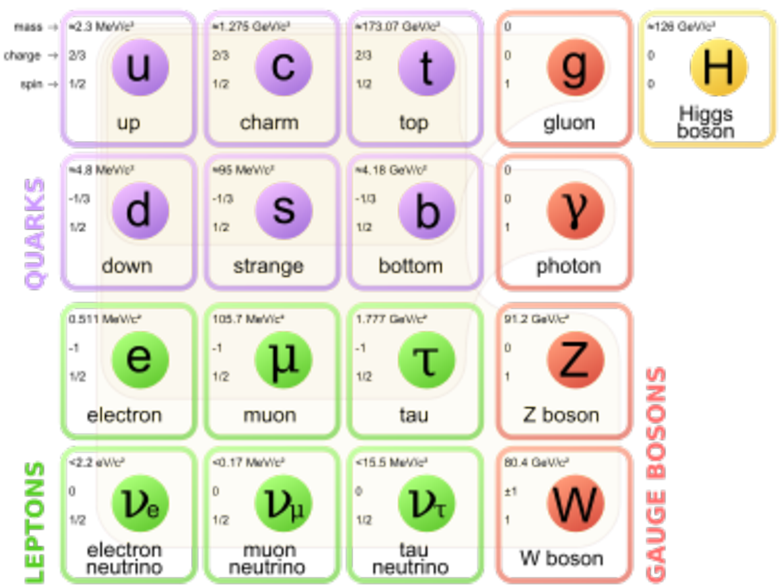
\includegraphics[width=0.8\textwidth]{intro/figs/Standard_Model_of_Elementary_Particles.pdf}
    \caption{
      \label{fig:SM}
      A diagram is shown with the particles making up the Standard Model along with the attributes of each particle.
    }
  \end{center}
\end{figure}

R-parity is a concept that is defined in equation~\ref{eqn:rparity} where B = baryon number, L = lepton number, and s = spin. 
Baryon number is defined in equation~\ref{eqn:baryonnumber},
where $\mathrm{N_{q}}$ and $\mathrm{N_{\bar{q}}}$ are the number of quarks and anti-quarks respectively.
Lepton number is defined in equation~\ref{eqn:leptonnumber},
where $\mathrm{N_{L}}$ and $\mathrm{N_{\bar{L}}}$ are the number of leptons and anti-leptons respectively.
All particles in the standard model have $\mathrm{R_{P}} = 1$.

\begin{equation}
\label{eqn:rparity}
\mathrm{P_{R} = (-1)^{3(B-L)+2s}}
\end{equation}

\begin{equation}
\label{eqn:baryonnumber}
\mathrm{B = \frac{1}{3}(N_{q}-N_{\bar{q}})}
\end{equation}

\begin{equation}
\label{eqn:leptonnumber}
\mathrm{L = N_{L}-N_{\bar{L}}}
\end{equation}

\subsection{Problems with The Standard Model}
The standard model is able to explain many things, but it is not complete.
One example of where it fails is in explaining the existence of ``dark matter''.
Dark matter is a form of matter that does not interact electromagnetically and has been observed by astrophysicists~\cite{darkmatter}.
Dark matter has been measured to be \textasciitilde{}5 times more abundant than visible matter in the universe.
The hierarchy problem is another question that is not explained by the standard model,
which essentially asks why is the weak force more than 1000 times stronger than gravity?
One of the main goals of particle physics is to understand and provide explanations for these problems,
and one way this can be done is within the context of supersymmetry (SUSY).

\section{Supersymmetry (SUSY)}
SUSY~\cite{SUSYPrimer} is an idea which postulates that for every particle in the standard model,
there exists a supersymmetric partner which has the property that the partners to bosons is fermionic, and the partners to fermions are bosonic.
These particles are named sparticles, and for fermions, an s, short for scalar, is added to the beginning of the standard model particle name to represent the SUSY particle.
A diagram of this is shown in figure~\ref{fig:SM_SUSY}.
For example, a supersymmetric electron is known as a selectron, and a supersymmetric quark is known as a squark.
For gauge bosons, the end of the name is changed to contain ``ino''.
For example, the supersymmetric partner to the W boson is known as the Wino and a supersymmetric gluon is known as a gluino.
R-parity is an important concept within SUSY, and all SUSY particles have $\mathrm{R_{P}} = -1$.
This means that if R-parity is conserved, the lightest supersymmetric particle (LSP) in a decay is stable.
The LSP then makes a good candidate for dark matter.
Using SUSY as a framework, one can create many models that can answer both the hierarchy problem as well as explain the existence of dark matter.
This thesis focuses more on a search for new physics within SUSY that can be used as an explanation for dark matter.

\begin{figure}[!htb]
  \begin{center}
    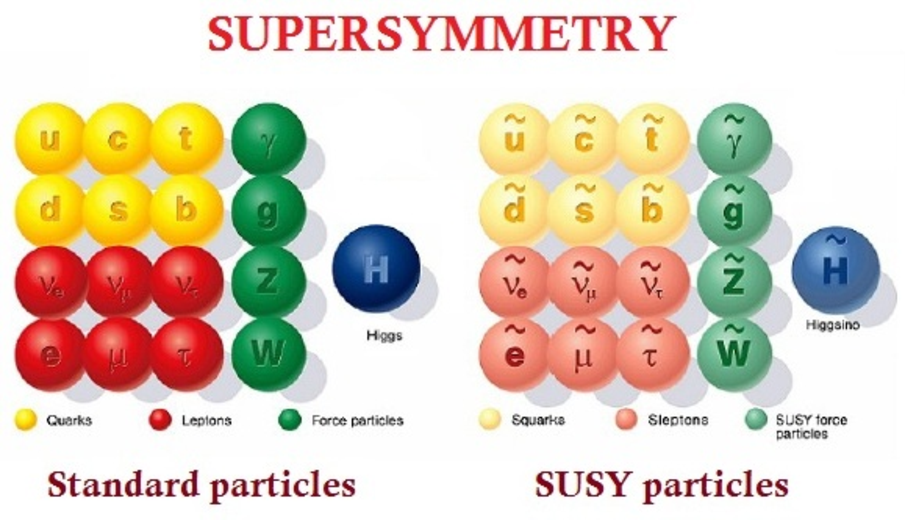
\includegraphics[width=0.8\textwidth]{intro/figs/Susy-particles.pdf}
    \caption{
      \label{fig:SM_SUSY}
      A diagram is shown with the particles making up the Standard Model on the left, and their SUSY counterparts on the right.
    }
  \end{center}
\end{figure}

%% \subsection{Gauge-Mediated Supersymmetry Breaking (GMSB)}
%% Gauge-Mediated Supersymmetry Breaking (GMSB) is a mechanism that allows supersymmetry to be broken.
%% This mechanism postulates the existence of a particle that can be used to explain gravity as well as dark matter, the gravitino ($\mathrm{\tilde{G}}$).
%% Within SUSY, the hierarchy problem can be solved with one loop corrections coming from heavy stop quarks,
%% and another consequence of GMSB is the proposal that stop quarks must have a mass greater than 2 TeV if the Higgs mass is 125 GeV.
%% The current upper limits on the mass of the stop squarks based on observations made by the CMS detector are around 800 GeV~\cite{stop2015}, as seen in figure~\ref{fig:T2tt_limits}.

%% \begin{figure}[!htb]
%%   \begin{center}
%%     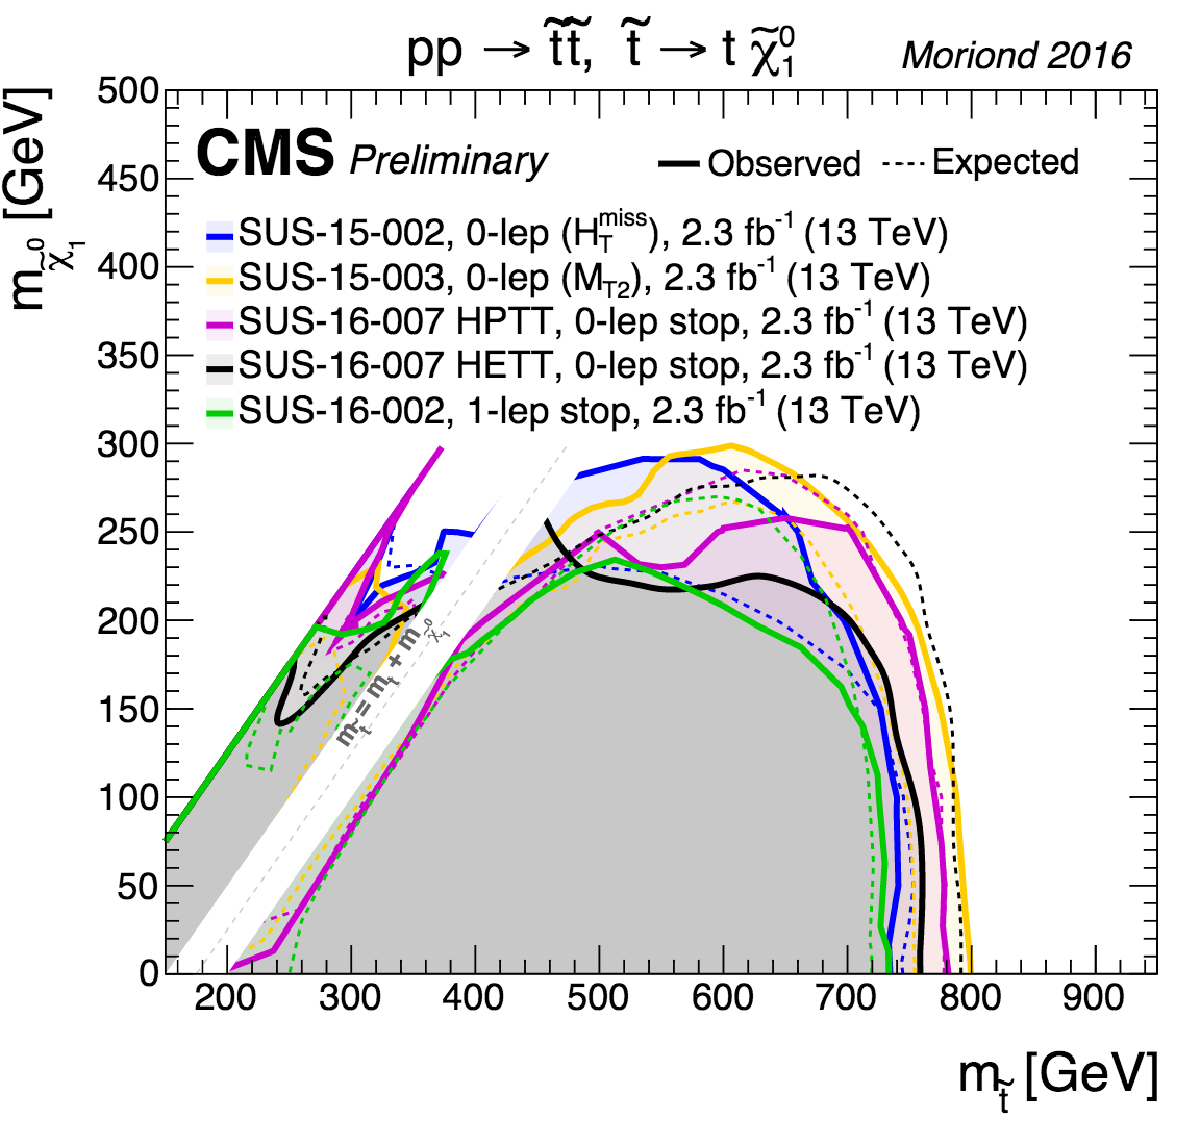
\includegraphics[width=0.8\textwidth]{intro/figs/T2tt_moriond2016.pdf}
%%     \caption{
%%       \label{fig:T2tt_limits}
%%       Exclusion limit on the SUSY final states where two stop squarks are pair-produced are shown,
%%       where the region in gray has been excluded by data taken by the CMS experiment.
%%     }
%%   \end{center}
%% \end{figure}

\section{Searches for SUSY in final states with a Z boson}
\label{sec:signalmodel}
Many models can exist within the context of SUSY, leading to a nearly endless variety of final states.
There are many parameters within SUSY that can be tuned to allow for the existence of different final states, for example the mass of the SUSY particles.
A set of simplified models can be described to get a sense of what possible final states can be probed using the CMS detector at the LHC.
These models are named SMS models, where SMS stands for Simplified Model Space~\cite{sms}.
One of these models, shown in figure~\ref{fig:SMS_T5ZZgmsb}, is a model with a final state containing two Z bosons,
four quarks and two invisible SUSY particles where the invisible particles in this model are the gravitino.
This thesis focuses on a search done using data taken by the CMS detector at the LHC colliding protons with a center of mass energy of $\mathrm{\sqrt{s}=13 TeV}$.
The next chapter will explain in detail how particles are measured using the CMS detector.

\begin{figure}[!htb]
  \begin{center}
    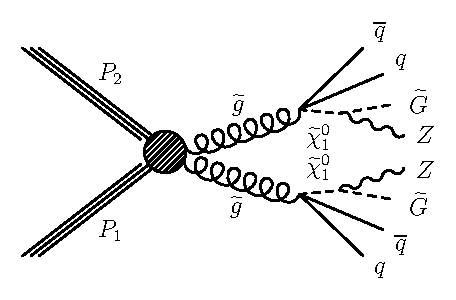
\includegraphics[width=0.8\textwidth]{intro/figs/Feynman_graph_T5ZZgmsb.pdf}
    \caption{
      \label{fig:SMS_T5ZZgmsb}
      A diagram showing a SUSY process where two protons collide and the result is pair-production of two gluinos,
      where each decays to a pair of quarks and a neutralino which subsequently decays to a Z boson and gravitino.
    }
  \end{center}
\end{figure}

% --------------------------------------------------------------------------- %
% --------------------------------------------------------------------------- %
\chapter{The LHC and The CMS Experiment}
\label {ch:cms}

\section{The Large Hadron Collider}
The Large Hadron Collider (LHC) is the largest particle accelerator in the world~\cite{lhcmachine}.
It is designed to collide protons against other protons with a center of mass energy up to 14 TeV.
The first collisions used for physics happened in March 2010, when the LHC was running at a center of mass energy of 7 TeV.
The LHC was restarted the following year and operated at a higher energy of 8 TeV
eventually delivering about four times the amount of data that was taken at 7 TeV.
After the successful first run ended, the machine was shut down in order to upgrade many components.
The next time the LHC was run was in May 2015, where protons were successfully collided at a center of mass energy of 13 TeV.
The analysis shown in this thesis is based on the data taken during the 2015 running period at 13 TeV.

In order to achieve such large center of mass energies,
the protons are accelerated in two separate circular beam pipes which are 27 km long and and 100 m underground.
These beam pipes are kept as close as possible to vacuum in order to minimize the interaction of protons with other particles.
Since the pipe is circular,
it's possible to accelerate two beams of protons in opposite directions and repeatedly collide them at various points around the ring.
There are 4 points along the ring where protons are made to collide and the resulting collisions are recorded by various experiments as seen in figure~\ref{fig:lhcunderground}.
The Compact Muon Solenoid (CMS) experiment~\cite{jinst} is where the data was taken used for the results shown in this thesis.

\begin{figure}[!ht]
  \begin{center}
    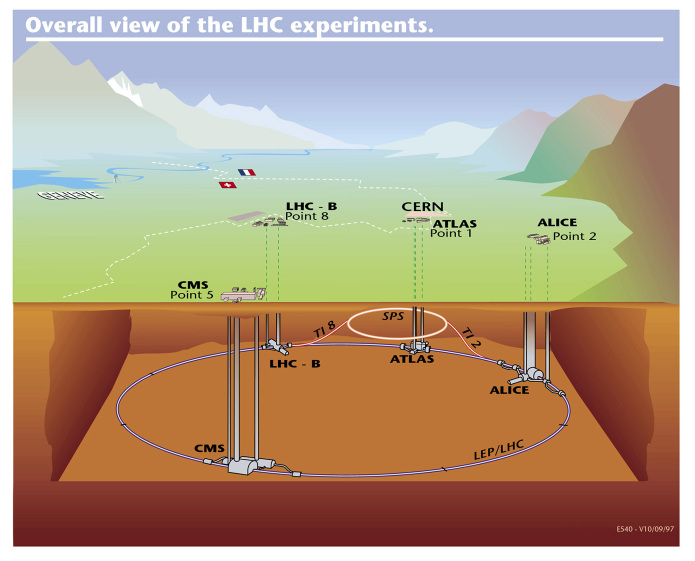
\includegraphics[width=0.8\textwidth]{cms/figs/lhc-underground.jpeg}
    \caption{ The LHC can be seen along with the 4 main experiments at different points along the beamline.
      \label{fig:lhcunderground}
    }
  \end{center}
\end{figure}

\section{Physics Processes and Cross Sections}
Particle physics processes are studied by measuring various quantities such as particle masses,
lifetimes, and production rates both inclusively and differentially with respect to certain kinematic variables.
When protons collide,
it is not the protons themselves that interact but rather the constituents, or partons, that make up the proton.
The formula describing this is given in equation~\ref{eqn:nevts}.
The number of events expected for a specific physics process is given by three quantities.
The integrated luminosity ($\mathcal{L}$) is dependent on the brightness of the proton beam.
The cross section for the event to happen ($\sigma$),
which includes the branching fraction for a particle to decay to a specific final state,
is a fundamental physics quantity.
the units for cross section is ``barns'', and a barn is defined as $\mathrm{10^{-24}~cm^{2}}$.
Lastly, the efficiency for the event to be reconstructed ($\epsilon$) is completely determined by the detector.

\begin{equation}
\label{eqn:nevts}
  \mathrm{N_{events} = \mathcal{L} * \sigma * \epsilon}
\end{equation}

Protons can interact elastically (scattering) or inelastically, meaning they are destroyed in the process.
The inelastic cross section for two protons to collide at a center of mass energy of 13 TeV is about 100 mb.
This can be seen in figure~\ref{fig:xsecs} along with the cross section values for other interesting
standard model processes.
Other processes that are main backgrounds in the signal region of this analysis are Drell-Yan and $\mathrm{t\bar{t}}$ production
which have a cross section at 13 TeV of roughly 4 nb, and 0.8 nb respectively.
Taking into account all the branching fractions and detector efficiencies,
these processes are reconstructed roughly once in a billion (trillion) times per inelastic proton collision for Z ($\mathrm{t\bar{t}}$) production.

\begin{figure}[!ht]
  \begin{center}
    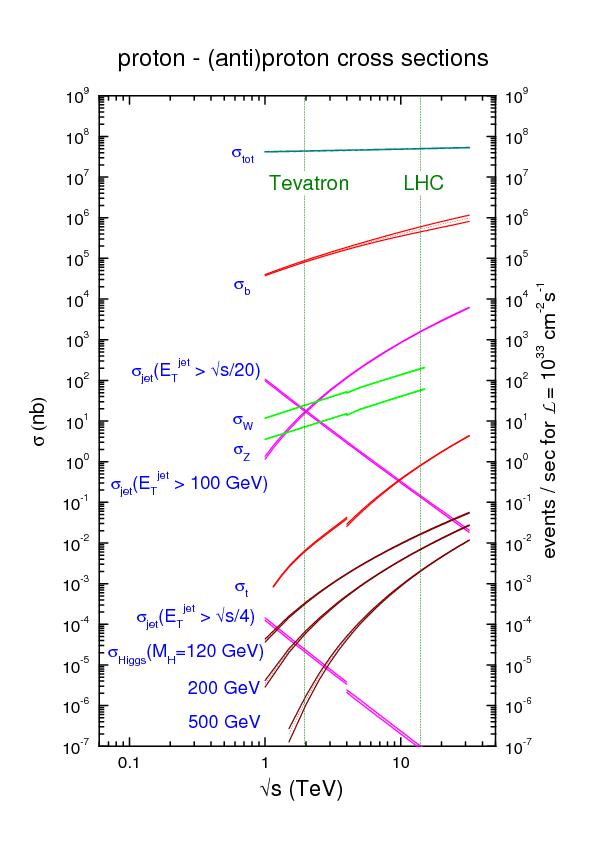
\includegraphics[width=0.8\textwidth]{cms/figs/cross-sections.png}
    \caption{
      The cross section values for various standard model processes is shown in this figure as a
      function of the center of mass energy of two protons colliding.
      \label{fig:xsecs}
    }
  \end{center}
\end{figure}

The peak instantaneous luminosity measured in a given day during the 2015 data taking period is shown on the left in figure~\ref{fig:peaklumi},
and the highest value is 5.13 $\mathrm{\frac{Hz}{nb}}$.
This means that approximately $\mathrm{10^{8}}$ protons collide per second.
The rate of collisions is much larger than the capacity for the detector to write out data,
and as discussed previously, most of these events are just soft inelastic collisions of two protons.
In order to maximize the efficiency of collecting data that is useful to any physics analysis,
a triggering system is put in place which only writes out the event information if certain conditions are met.
The maximum rate of all the concurrent triggers in CMS is about 1 kHz.
The total luminosity collected in 2015 was 3.81 $\mathrm{fb^{-1}}$ which can be seen on the right in figure~\ref{fig:peaklumi},
but due to data quality issues the amount that was useable for physics analysis was 2.26 $\mathrm{fb^{-1}}$.

\begin{figure}[!ht]
  \begin{center}
    \begin{tabular}{c c}
      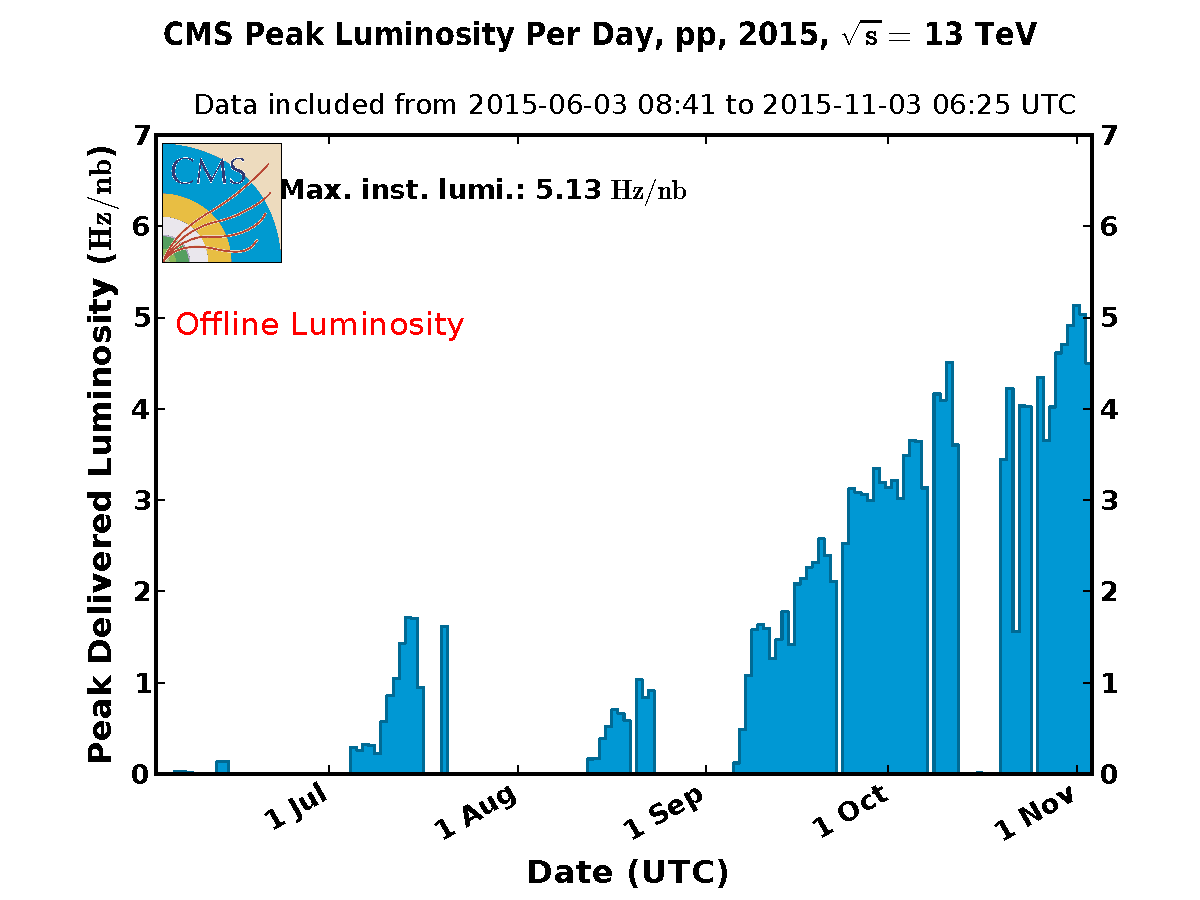
\includegraphics[width=0.4\textwidth]{cms/figs/peak_lumi_per_day_pp_2015.pdf} &
      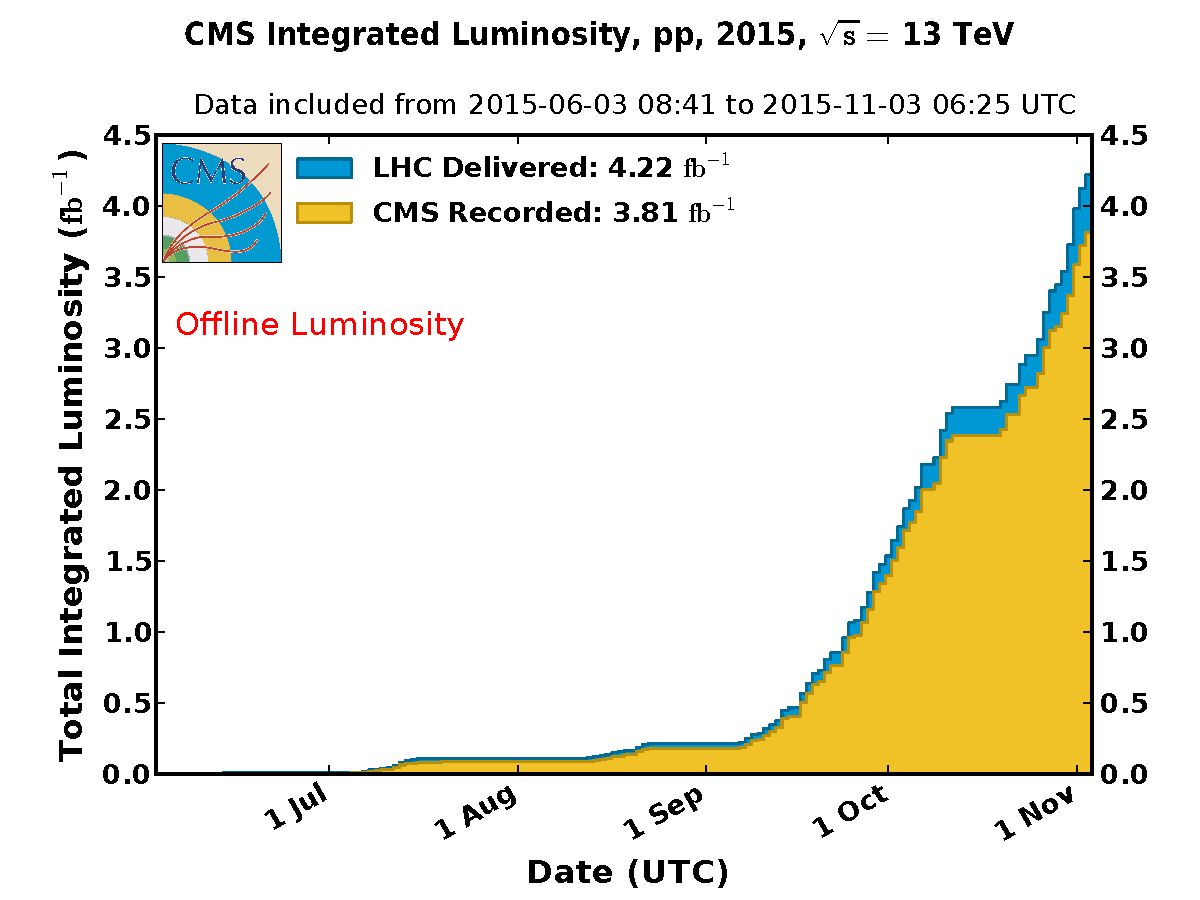
\includegraphics[width=0.4\textwidth]{cms/figs/int_lumi_per_day_cumulative_pp_2015.pdf} \\      
    \end{tabular}
    \caption{
      The peak instantaneous luminosity per day during the 2015 data taking period is shown on the left
      and the total integrated luminosity is shown on the right in this figure.
      \label{fig:peaklumi}
    }
  \end{center}
\end{figure}

\section{Particle Interactions With Matter}

The total amount of energy lost by a particle when interacting with matter is mainly due to two effects,
interactions that lead to the particle decaying or ``showering'',
and energy loss by ionization.
Two equations are used to describe energy loss due to showering,
equations~\ref{eqn:radiation_length} describes particle interactions via QED processes,
and~\ref{eqn:interaction_length} describes particle interactions via QCD processes.
Equation~\ref{eqn:radiation_length} represents the average energy left over as a particle travels a distance x through a material with radiation length ($X_{0}$).
Equation~\ref{eqn:interaction_length} represents the average number of particles left when $N_{0}$ particles traverse a distance x through a material with interaction length ($\lambda_{int}$).
The largest source of uncertainty when measuring a particle's energy using the ECAL or HCAL is called the ``stochastic term''
and is mostly due to intrinsic statistical shower fluctuations and sampling fluctuations.
The energy of a parton is distributed evenly among all of its decay products on average,
so the initial particles energy is proportional to the number of decay products $E_{0} \propto N_{0}$.
The overall uncertainty due to the stochastic term becomes proportional to $\sqrt{N_{0}}$ in the limit where N is large.

\begin{equation}
  \label{eqn:radiation_length}
  E(x) = E_{0}e^{\frac{-x}{X_{0}}}  
\end{equation}

\begin{equation}
  \label{eqn:interaction_length}
  N(x) = N_{0}e^{\frac{-x}{\lambda_{int}}}  
\end{equation}

Typical values for radiation and interaction lengths are shown in table~\ref{tab:rad_int_lengths}
for the different materials making up the tracker (silicon), ECAL (PbWO4) and HCAL (Copper).
In table~\ref{tab:materialbudget}, the depth of each of these materials corresponding to $|\eta| = 0$ is shown as a function of $X_{0}$ and $\lambda_{int}$.
The values in tables~\ref{tab:rad_int_lengths}~and~\ref{tab:materialbudget} are taken from a talk given at CERN in May 2016~\cite{calorimetry}.
Based on these values, an electron or photon loses at least \textasciitilde{}40\%
of its energy on average when traveling through the tracker before it is incident on the ECAL.
This means either has a relatively high chance of interacting, where a photon might pair-produce and an electron might brem a photon.
These effects are taken into consideration when reconstructing photons and electrons and better-described in chapter~\ref{ch:evtsel}.

Another effect that can be seen is in the HCAL, which is a ``sampling'' calorimeter.
A sampling calorimeter is designed to have layers of material with large
$\lambda_{int}$~interpsered with layers of material that are used to measure particles.
This is described in more detail in subsection~\ref{subs:HCAL}.
In the HCAL in CMS, there are 16 layers of absorber material.
This means that each layer has more than 4.5 radiation lengths.
When a hadronic shower evolves, approximately 30\% of the shower is in the form of EM energy.
4.5$\mathrm{X_{0}}$ is essentially deep enough to completely contain the EM component of the hadronic shower before it can be measured.
This leads to an increased uncertainty of the initial parton's energy.

\begin{table}[htb]                                                                                                                                                              
  \begin{center}
    \caption{
      \label{tab:rad_int_lengths}
      Radiation ($\mathrm{X_{0}}$) and interaction lengths ($\lambda_{int}$) for various materials that make up different sub-detectors in CMS.
    }
    \begin{tabular}{l|c|c}
      \hline
      \hline
      Material & $\mathrm{X_{0}}$ [cm] & $\lambda_{int}$ [cm] \\
      \hline
      Silicon                             & 9.36 & 45.5 \\
      Lead Tungstate (PbW$\mathrm{O_{4}}$) & 0.88 & 19.5 \\
      Copper                              & 1.43 & 15.1 \\
      \hline
      \hline
    \end{tabular}
  \end{center}
\end{table}

\begin{table}[htb]                                                                                                                                                              
  \begin{center}
    \caption{
      \label{tab:materialbudget}
      Material budget of tracker and calorimeters in CMS at $|\eta|=0$ as a function of radiation ($\mathrm{X_{0}}$) and interaction ($\lambda_{int}$) lengths.
    }
    \begin{tabular}{l|c|c}
      \hline
      \hline
      Material & Radiation lengths [$\mathrm{X_{0}}$] & Interaction lengths [$\lambda_{int}$]  \\
      \hline
      Silicon                             & 0.5 & 0.1 \\
      Lead Tungstate (PbW$\mathrm{O_{4}}$) & 25 & 1.1 \\
      Copper                              & 73.9 & 7 \\
      \hline
      \hline
    \end{tabular}
  \end{center}
\end{table}

Energy loss by ionization is mostly due to a particle having elastic collisions with electrons and can be characterized by the Bethe-Bloch formula shown in equation~\ref{eqn:bethebloch}.
In this equation, K is a constant equalling 0.307 MeV $\mathrm{g^{-1}}cm^{2}$,
$\mathrm{T_{max}}$ is the max energy transfer in a single collision,
$z$ is the charge of the incident particle,
Z is the charge number of the medium,
A is is the atomic mass of the medium,
$m_{e}$ is the mass of an electron,
and I is the mean excitation energy of the medium.
Muons have a low interaction cross section with the materials used to build CMS in the energy range that they are produced when coming from Z bosons produced at the LHC.
They are referred to as minimum ionizing particles, and the stopping power of copper on muons can be seen in figure~\ref{fig:muonenergyloss}.
Therefore, muons do not deposit very much energy in any of the calorimeters.
Typical momenta of muons in this analysis are between 20-200 GeV.
When muons have momenta greater than 200 GeV, radiative losses start to become the primary reason for energy loss.

\begin{equation}
  \label{eqn:bethebloch}
-<\frac{dE}{dx}> = Kz^{2}\frac{Z}{A}\frac{1}{\beta^{2}}[\frac{1}{2}ln\frac{2m_{e}c^{2}\beta^{2}\gamma^{2}T_{max}}{I^{2}}-\beta^{2}-\frac{\delta(\beta\gamma)}{2}]
\end{equation}

\begin{figure}[!htb]
  \begin{center}
    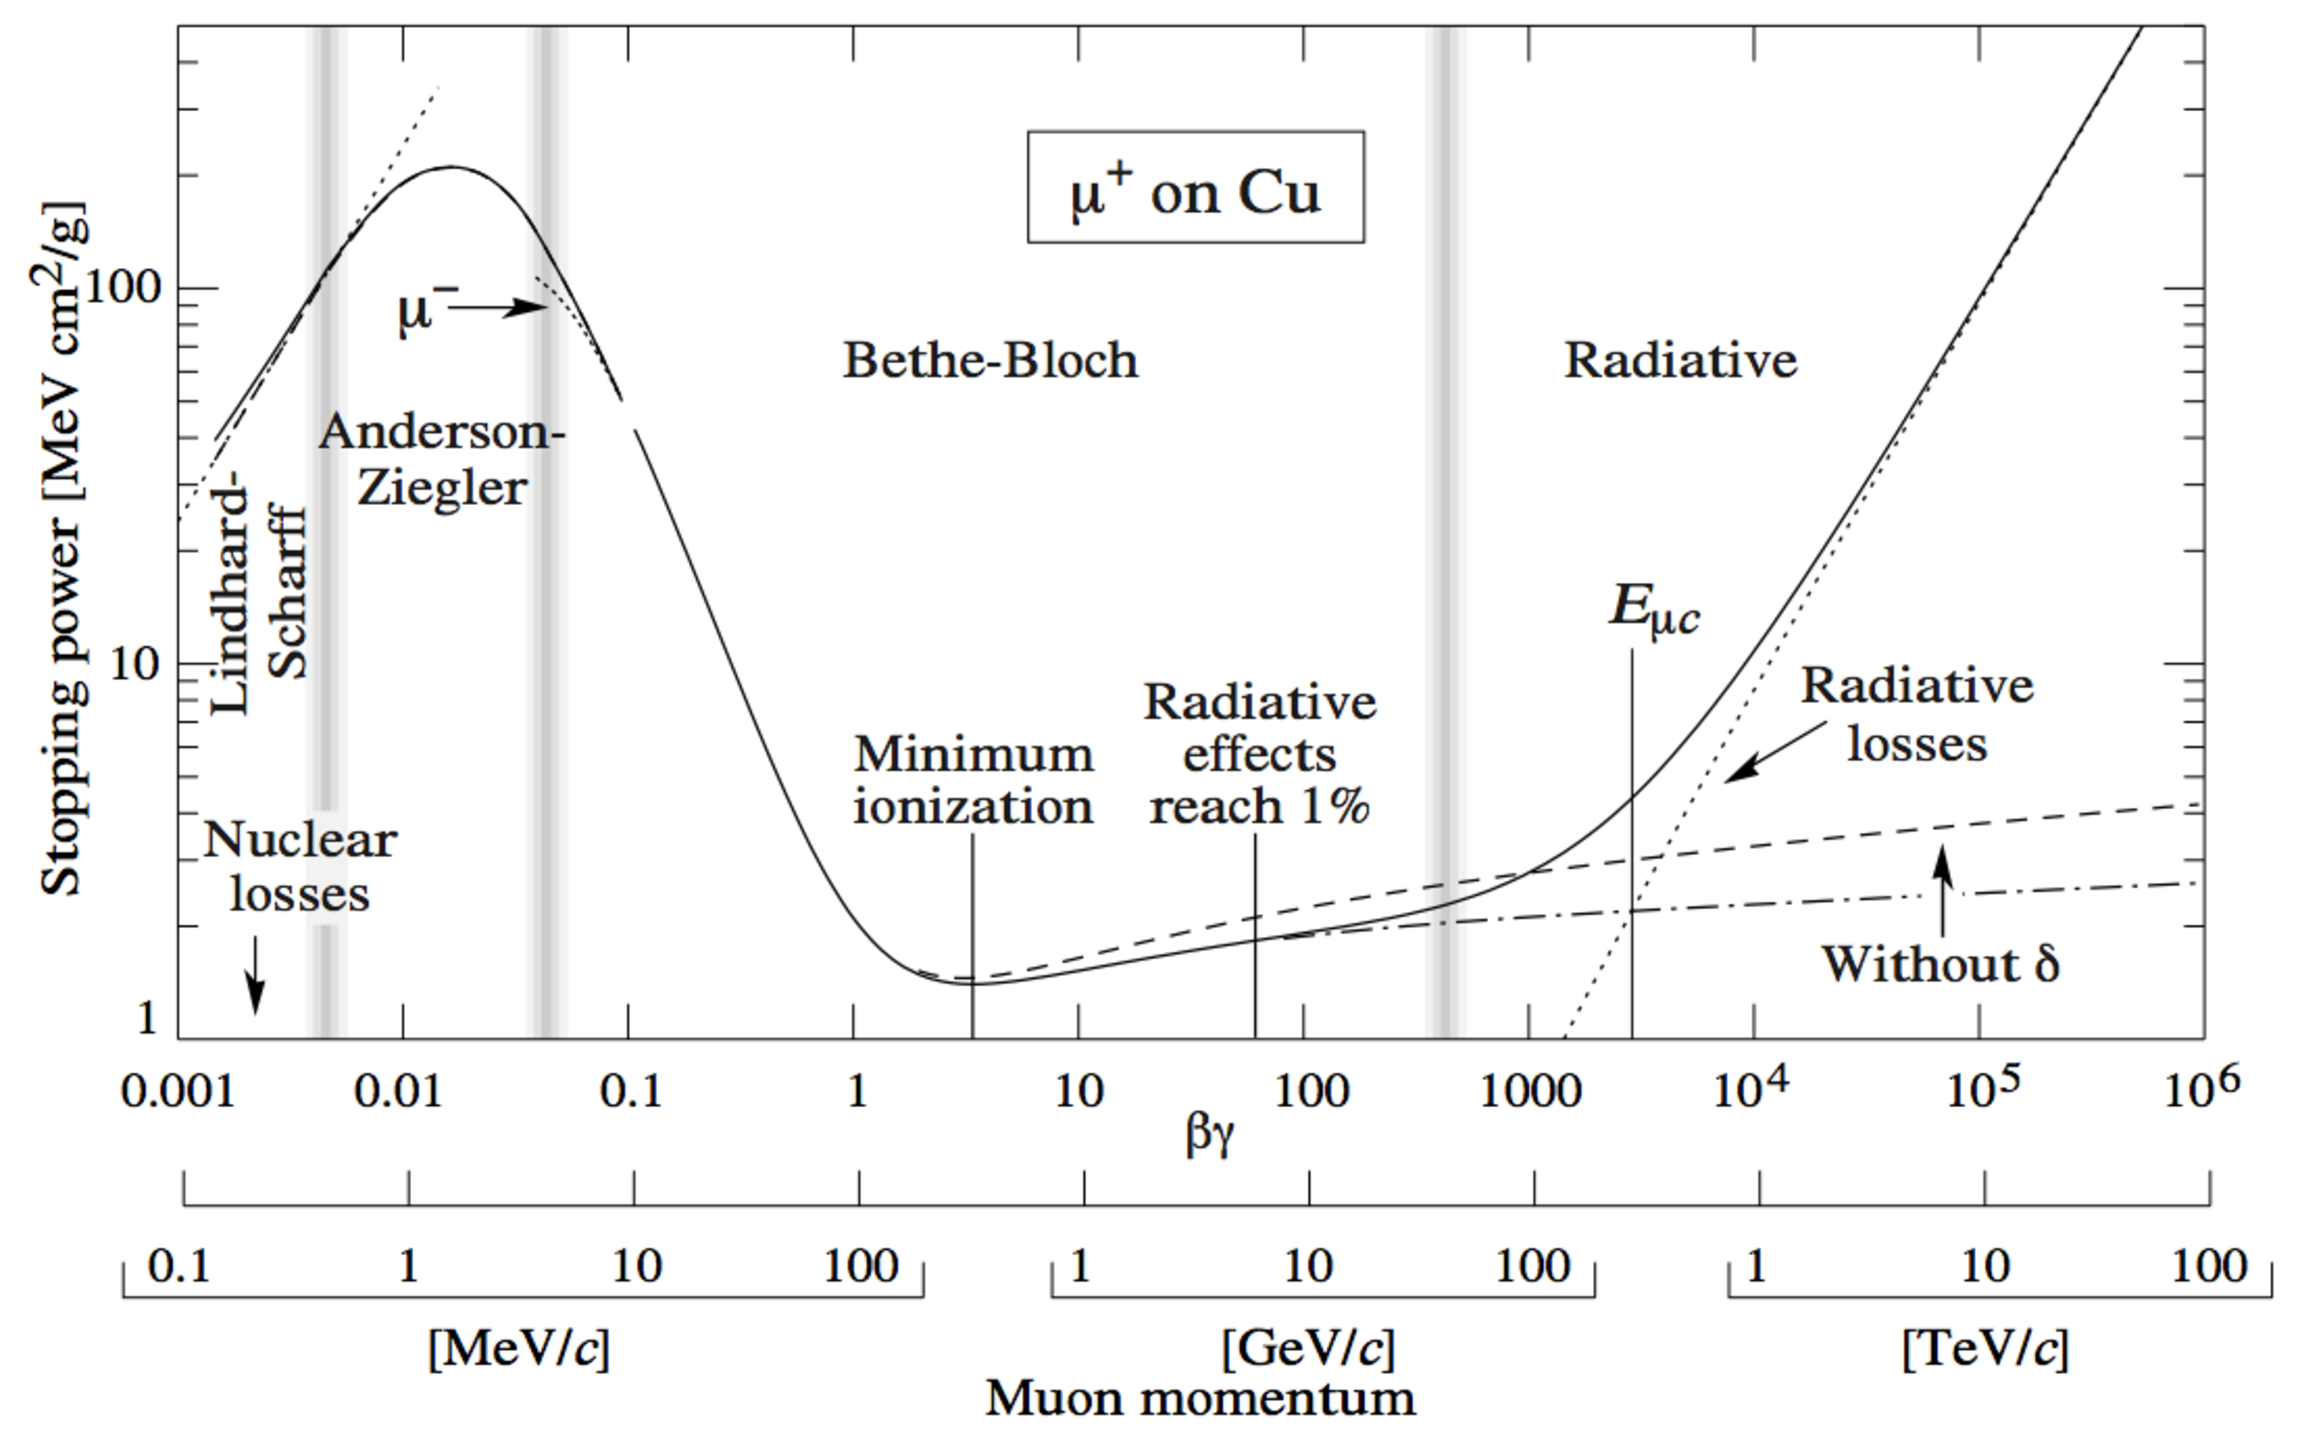
\includegraphics[width=0.8\textwidth]{cms/figs/muon_energy_loss.pdf}
    \caption{
      \label{fig:muonenergyloss}
      Stopping power of copper as a function of muon momentum. Typical momenta of muons in this analysis are between 20-200 GeV.
    }
  \end{center}
\end{figure}

\section{The Compact Muon Solenoid}
The CMS detector consists of a triggering system and many sub detectors,
where measurements taken using these sub detectors are used as input to the triggering system.
When protons are collided at the interaction point within CMS, approximately N collisions happen per second.
The rate of collisions is so high that it is impossible to record all of the data all of the time.
The way this is controlled is by the use of triggers, the level 1 (L1) trigger and the high level triggers (HLT).
The triggers are designed such that the full event information is stored when all the requirements of a trigger are met.
For some physics processes, trigger rates are much higher than can be afforded by the allowed budget of the CMS experiment.
These processes can still be studied by prescaling the triggers meaning the full information is saved once per N events.
As the prescale N is increased, the rate of the trigger is reduced.

The CMS sub detector components are layered in such a way that one can take advantage of different particle interactions with different materials.
The innermost layer is the tracker (decribed in section~\ref{subs:tracker}) which is used to measure the charge and momentum of charged particles.
When a charged particle passes through the silicon tracker's layers, a small amount of energy is deposited.
The deposit is large enough that a hit will be registered by the electronics, but small enough that the trajectory of the particle will be minimally affected.

The next layer is the Electromagnetic Calorimeter (decribed in section~\ref{subs:ECAL}) which is used to contain and measure the energy of electrons and photons.
The Electromagnetic Calorimeter (ECAL) is made of lead tungstate ($\mathrm{PbWO_{4}}$) scintilating crystals.
Electrons and photons that enter the ECAL lose energy due to showering, and the depth of the ECAL is sufficient enought to fully contain these particles.

Outside of the ECAL is the Hadronic Calorimeter (decribed in section~\ref{subs:HCAL}) which is used to contain and measure the energy of hadronic particles.
The Hadronic Calorimeter (HCAL) is designed in such a way that hadronic particles incident on the HCAL lose energy to showering.
The goal is to fully contain these particles, although sometimes particles have sufficient energy that they are able to escape before losing sufficient energy to showering.
This phenomenon is known as punch-through.

Beyond the HCAL is the solenoid which produces a magnetic field of 3.8 T at the center of the detector.
This magnetic field is used to bend the tracks of charged particles in order to measure the momentum following the equation~\ref{eqn:bfieldmomentum},
where q is the particle charge, r is the radius of curvature, and B is the magnetic field magnitude.

\begin{equation}
  \label{eqn:bfieldmomentum}
p = qrB
\end{equation}

The only particles that should pass beyond the HCAL are muons and neutrinos.
Neutrinos are measured indirectly by assuming that the momentum in the direction transverse to the beam is zero at the beginning of each collision,
and then calculating the sum of the total transverse momentum of all particles directly measuered in the detector.
Since Neutrinos pass through the detector with no interactions, they contribute to missing transverse momentum, which will be referred to as (\MET) or MET.

Lastly, the muon system (decribed in section~\ref{subs:MUON}) is used to measure the charge and momentum of muons.
At the energies that muons are most commonly produced in collisions at the LHC, muons are minimum ionizing particles (MIPs)
meaning they do not lose very much energy as they pass through the detector components.


\subsection{Silicon Tracker}
\label {subs:tracker}
The tracker, shown in figure~\ref{fig:tracker}, has two main components, the pixels and the strips.
The pixel component has three cylindrical layers very close to the beam pipe, which are positioned at 4, 7 and 11 cm from the center.
The pixel detector contains over 65 million sensors (pixels) measuring 150 by 150 $\mu$m which are connected directly to a chip used to read out the data.
A diagram showing the pixels can be seen in figure~\ref{fig:pixels}.
When a charged particle travels through the three pixel layers,
the hits are recorded then used together with the measurement of the particle's trajectory through the strip component of the tracker.

\begin{figure}[!htb]
  \begin{center}
    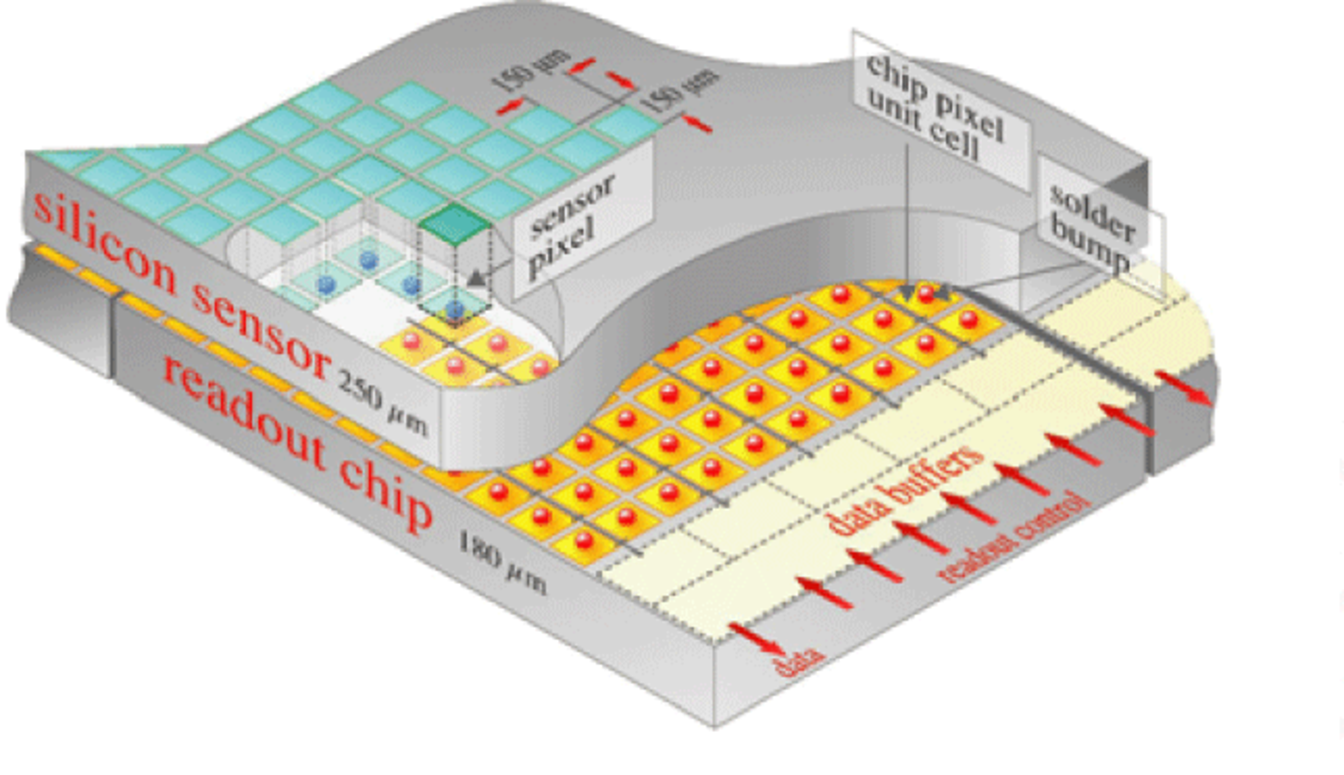
\includegraphics[width=0.8\textwidth]{cms/figs/Pixelement.pdf}
    \caption{
      \label{fig:pixels}
      A diagram showing the pixel component of the tracker subdetector.
    }
  \end{center}
\end{figure}

Immediately outside of the pixel layer is the strip layer.
There are 10 layers of strips through which a charged particle passing through will leave deposits of energy that are read out.
The very large magnetic field in this region from the solenoid is in the same direction as the beam,
and this causes particle trajectories to curve in a direction tangent to the beam direction. 
The radius of this curvature is proportional to the particle's momentum and inversely proportional to the particle's charge according to equation~\ref{eqn:bfieldmomentum}.
Using the hit information from the pixels and strips together,
the momentum of all the charged particles that pass through the tracker is reconstructed and
used as input to the particle flow algorithm~\ref{subs:particleflow} in order to identify particles produced in the collision.
The total material budget of the tracker as a function of radiation and interaction length is shown in figure~\ref{fig:trackerbudget}.
The total depth is seen to be increasing with $|\eta|$ up to where the tracker barrel meets the tracker endcap then decreasing after this point.

\begin{figure}[!htb]
\begin{center}
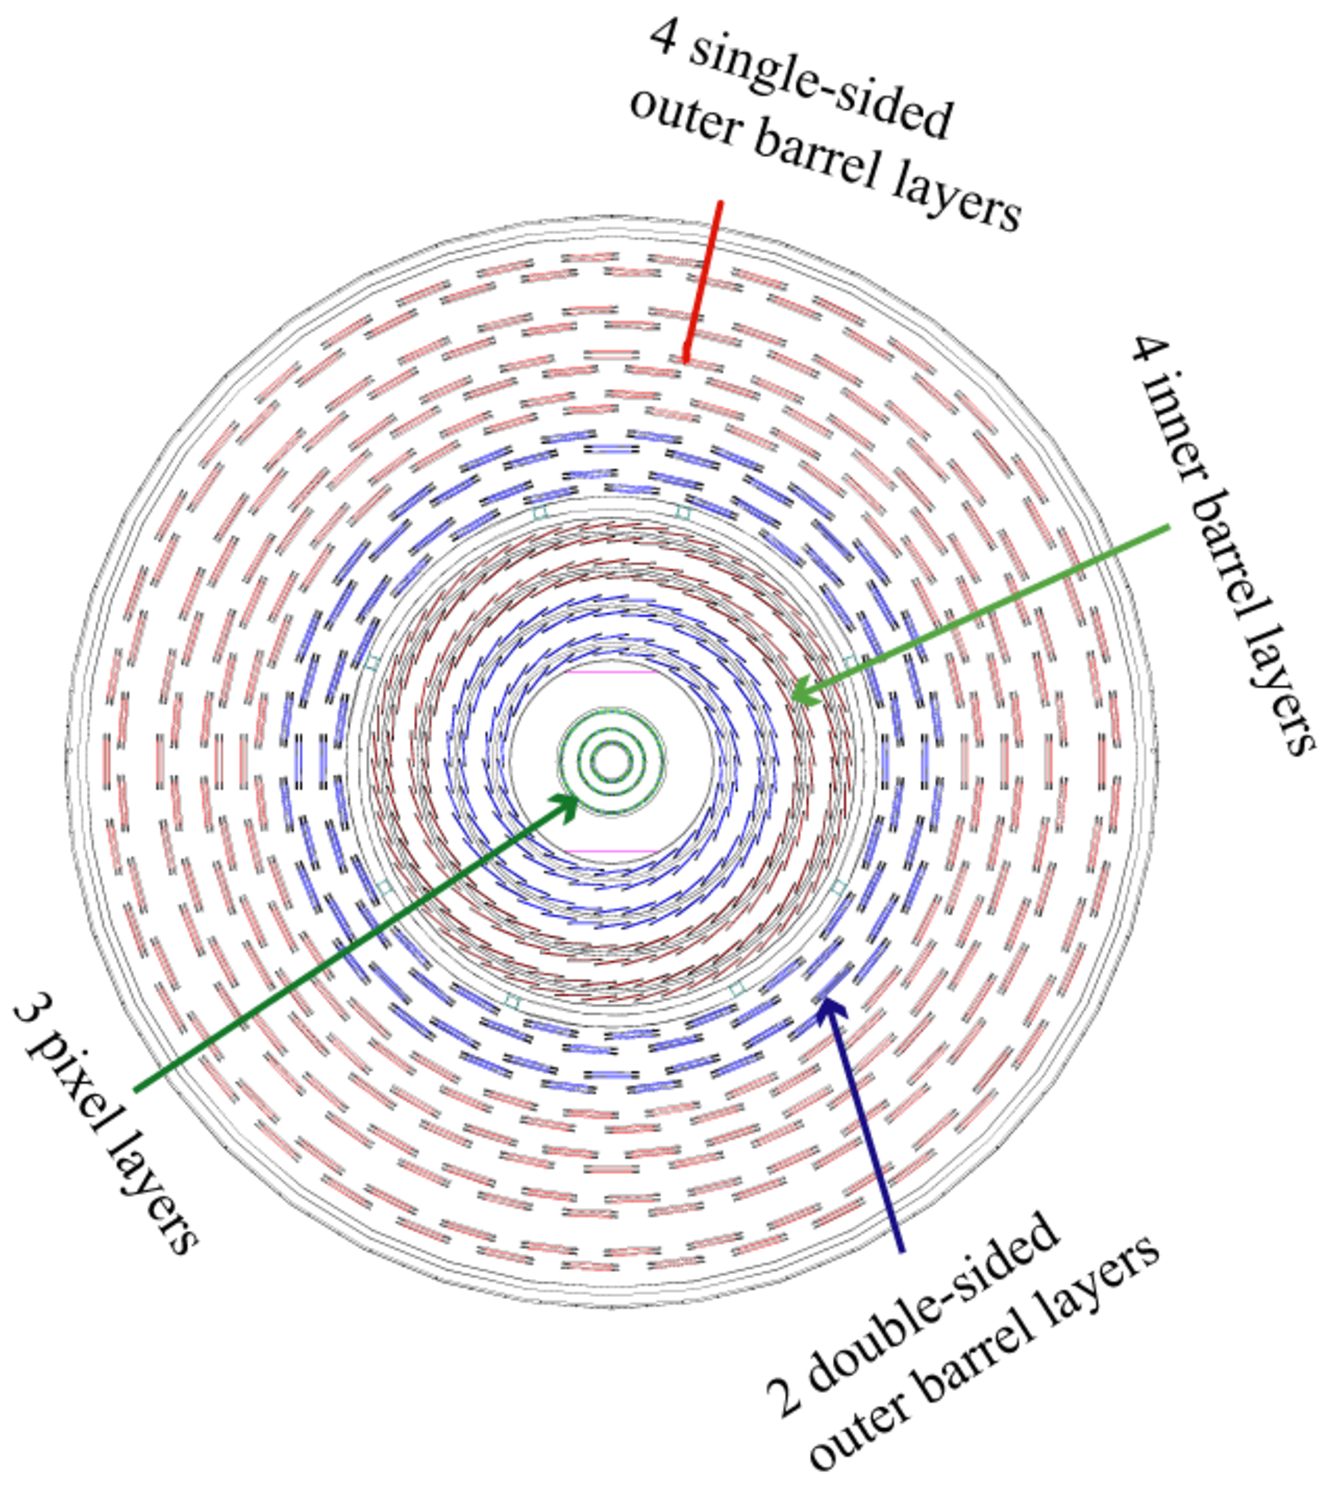
\includegraphics[width=0.8\textwidth]{cms/figs/Barrel.pdf}
\caption{
  A cross-sectional in the x-y plane of the CMS tracking system is shown here.
  The tracker provides excellent coverage for reconstruction of tracks from charged particles for $|\eta| < $2.5.
\label{fig:tracker}
}
\end{center}
\end{figure}

\begin{figure}[!htb]
  \begin{center}
  \begin{tabular}{c c}
    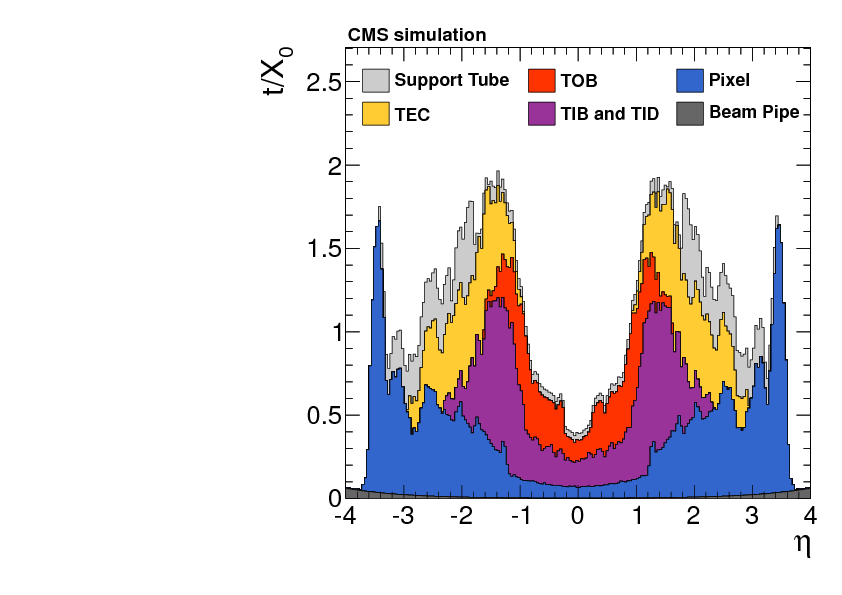
\includegraphics[width=0.4\textwidth]{cms/figs/figs_2011_cmsTracker_MaterialBudget_RadLengths.png} &
    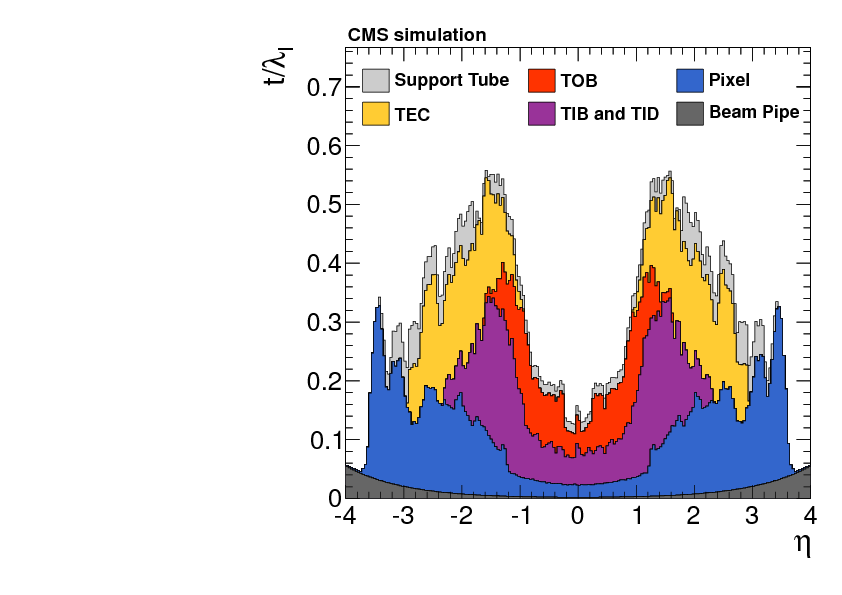
\includegraphics[width=0.4\textwidth]{cms/figs/figs_2011_cmsTracker_MaterialBudget_InteractionLengths.png} \\
  \end{tabular}
    \caption{
      \label{fig:trackerbudget}
      A diagram showing material budget of the tracker as a function of $\eta$ on the x-axis, and radiation lengths (left) and interaction lengths (right).
    }
  \end{center}
\end{figure}


\subsection{Electromagnetic Calorimeter}
\label {subs:ECAL}
The ECAL is split into two regions, the ECAL barrel (EB), and ECAL endcap (EE).
The EB occupies a region in the detector within $|\eta| < 1.479$, and the EE occupies the region with $1.479 < |\eta| < 3.0$.
The geometry can be seen in figure~\ref{fig:ecal_eta}.

\begin{figure}[!htb]
\begin{center}
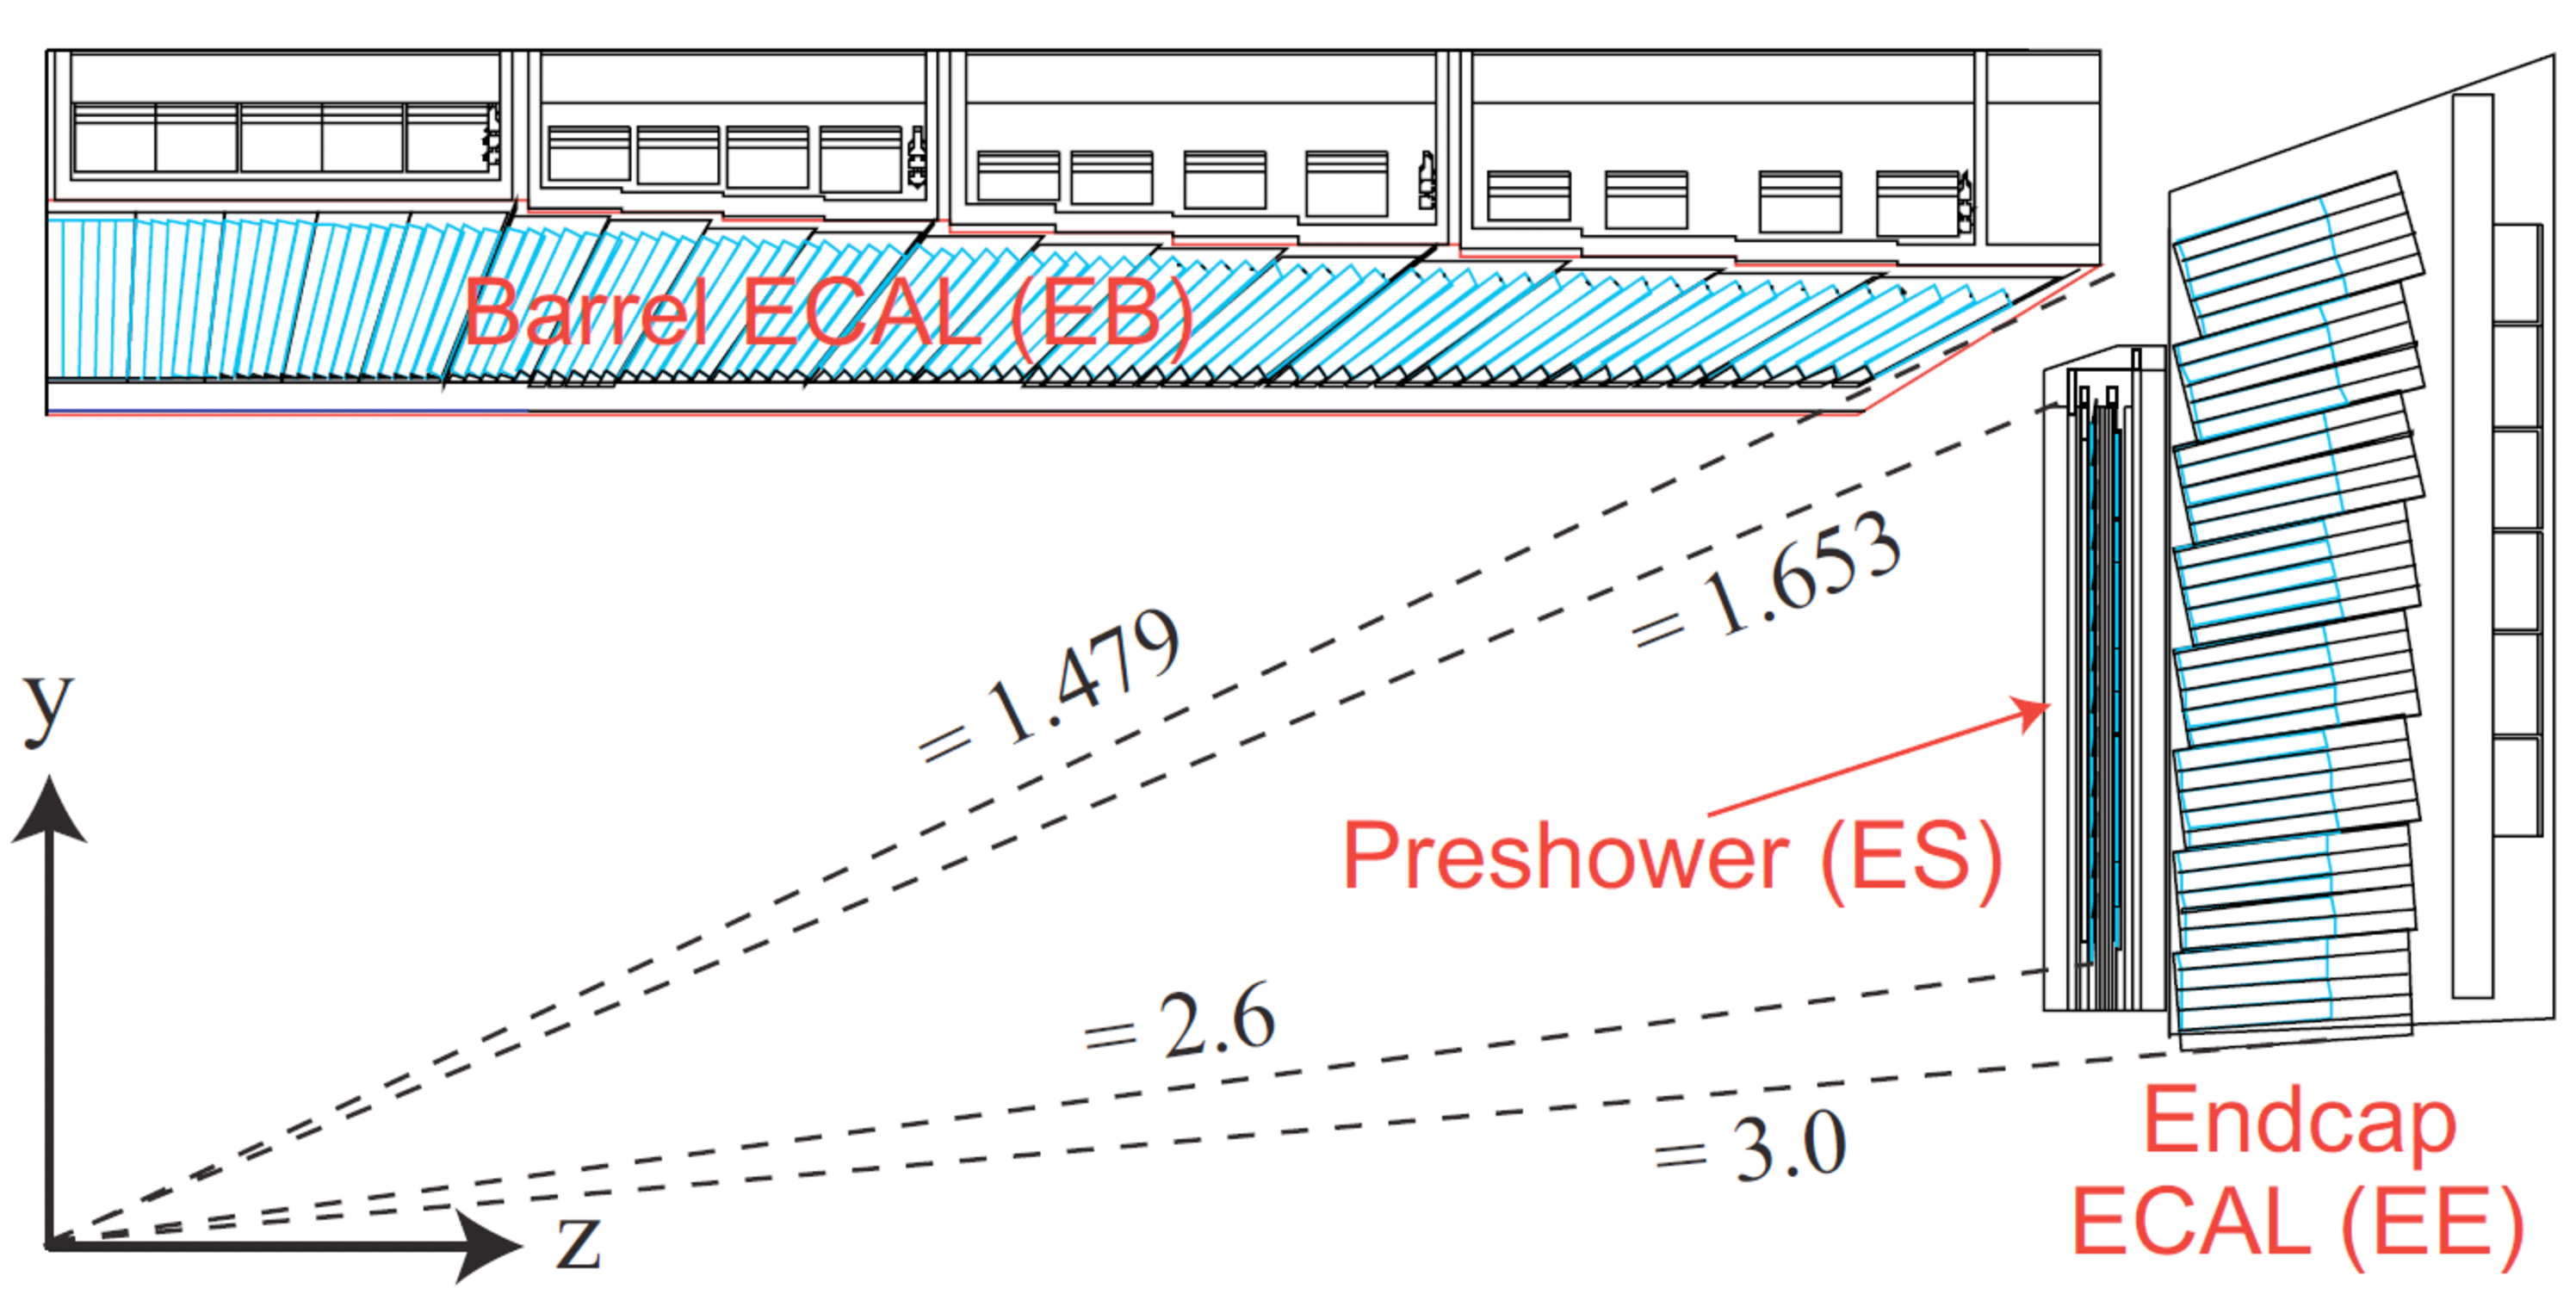
\includegraphics[width=0.8\textwidth]{cms/figs/Figures_Experimental_Apparatus_ECALRapidity.pdf}
\caption{ A cross-sectional view of the CMS ECAL is shown in this figure, with values of $\eta$ shown that determine the coverage of each subdetector.
\label{fig:ecal_eta}
}
\end{center}
\end{figure}

\clearpage

As written previously, the ECAL is made of lead tungstate crystals.
These crystals act as absorbers as well as scintilators.
What this means is that the when electrons or photons are incident on the crystals, they lose energy due to showering.
The showering process can be simply described as a combination of electron-positron pair production, and photon emission.
Leading order diagrams of these processes are shown in figures~\ref{fig:pair_production}~and~\ref{fig:photon_brem}.

\begin{figure}[!ht]
\begin{center}
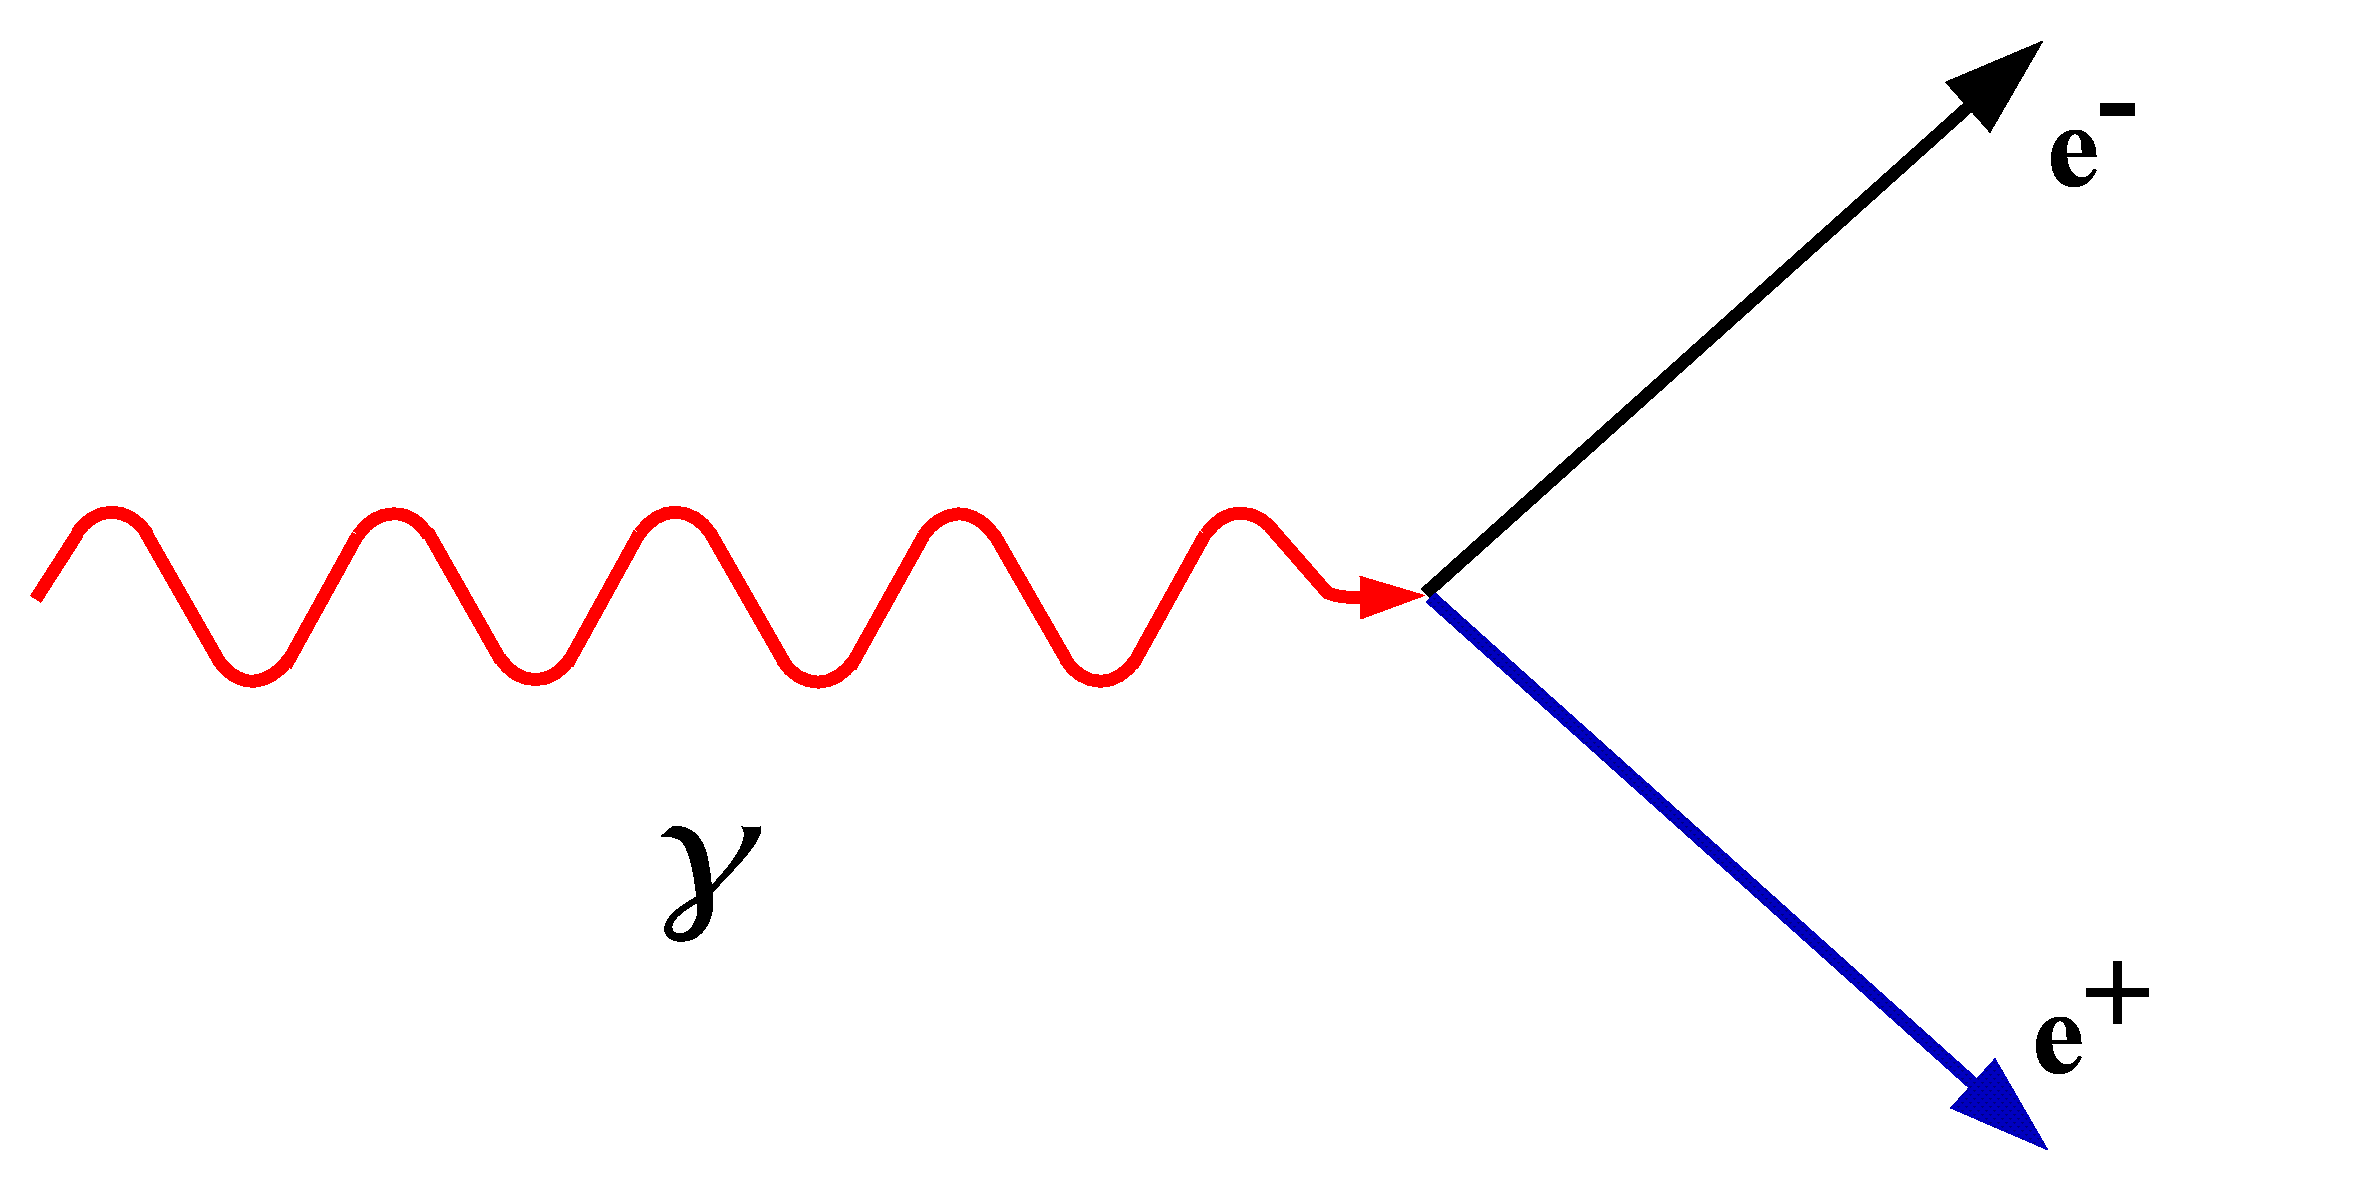
\includegraphics[width=0.8\textwidth]{cms/figs/Pair_Production.png}
\caption{ A feynman diagram is shown depicting electron-positron pair production from a photon initial state.
\label{fig:pair_production}
}
\end{center}
\end{figure}

\begin{figure}[!ht]
\begin{center}
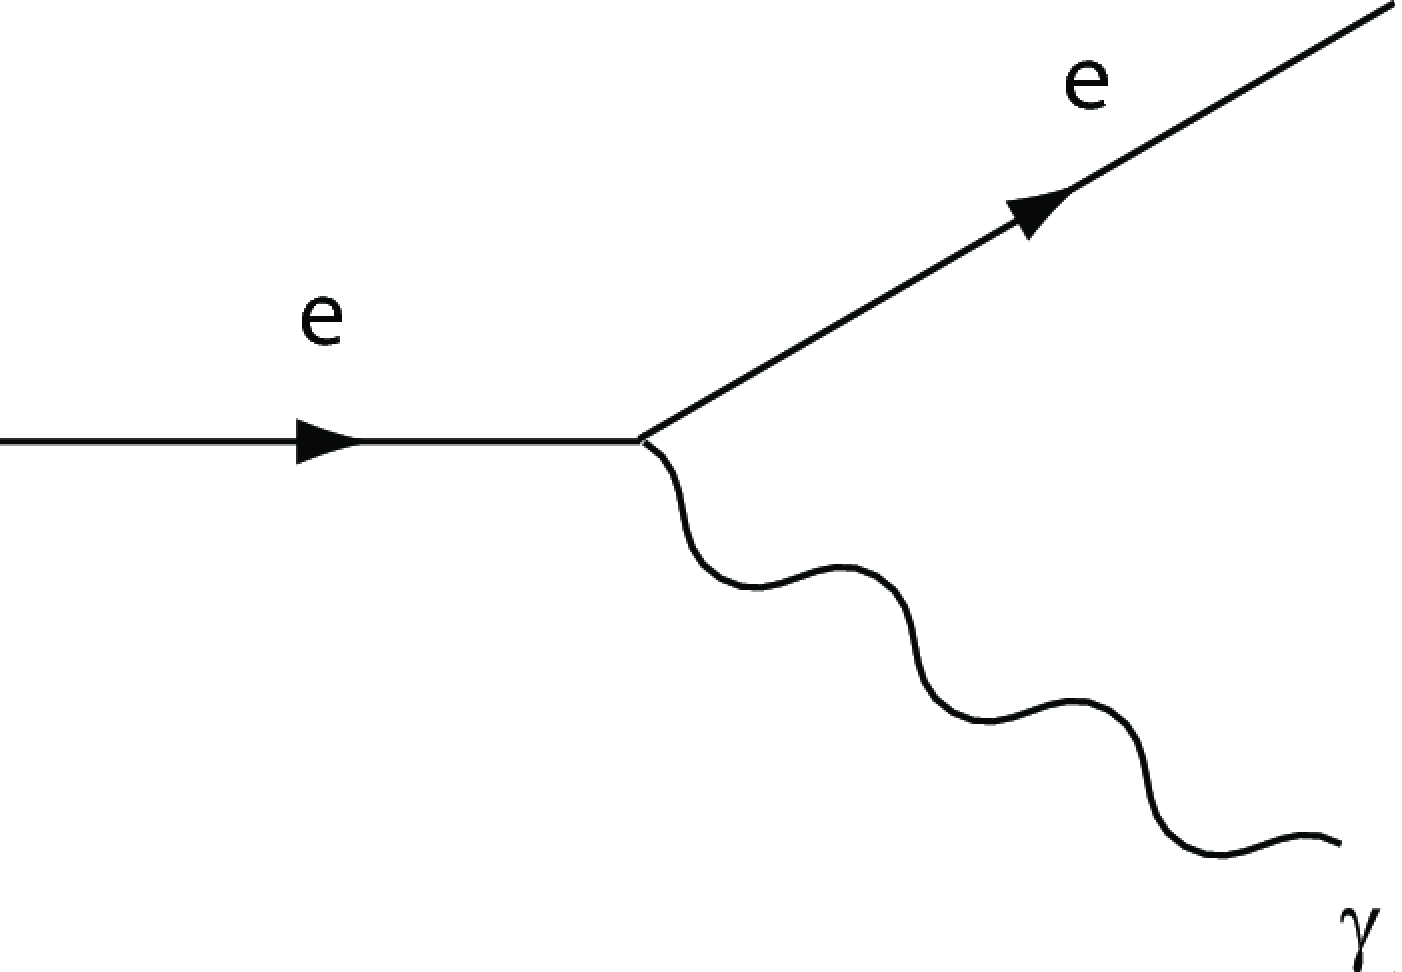
\includegraphics[width=0.8\textwidth]{cms/figs/photon_brem.png}
\caption{
  A feynman diagram is shown of a process where an electron radiates a photon through bremsstrahlung.
\label{fig:photon_brem}
}
\end{center}
\end{figure}

As the initial particle passes through the crystal, it loses energy due to these processes, and this energy is converted to light by the scintilating properties of the crystal.
This light is read out using a avalanche photo-diode (APDs) for each crystal in the EB, and a vacuum phototriode for each crystal in the EE.
The amount of energy absorbed by the crystals can be parameterized by a quantity known as the radiation length ($X_{0}$).
The expected amount of energy left (E(x)) after a particle with initial energy ($E_{0}$)
travels a distance x through an absorbing material is shown in equation~\ref{eqn:radiation_length}.
The CMS ECAL has a depth of \textasciitilde{}25$X_{0}$ at small (0-1.3) and large (1.6-3.0) values of $\eta$.
In between these regions, the depth is larger due to the barrel-like geometry of the ECAL.
Additionally, the ECAL material has a Moli\`ere radius ($\mathrm{R_{M} \simeq 2.19~cm}$) where
$\mathrm{R_{M}}$ is defined as the radius of a cylinder containing on average 90\% of the shower's energy deposition.
Because of the depth and intrinsic resolution, electron and photon energies are measured very well in the ECAL.
There is one exception where the depth of the ECAL is small, and this is where the barrel and endcap meet.
This leads to poor reconstruction of electrons and photons in this region.

\subsection{Hadronic Calorimeter}
\label {subs:HCAL}
The Hadronic Calorimeter (HCAL) is used to measure energies of hadronic particles, such as charged pions, gluons, protons, kaons and neutrons~\cite{hcalperformance}.
It is a sampling calorimeter meaning it has many layers of absorber material (brass) and scintilator material (plastic).
As hadronic particles pass through the HCAL, they interacts with the absorber layers by showering, meaning they decay to multiple lower energy particles.
As these particles shower and the constituents pass through the scintilator, photons are emitted by the scintilating material and then measured by Hybrid-Photo Diodes (HPDs).

When a hadronic particle is incident on the HCAL, a hadronic shower is induced.
Approximately two third of the particles produced in a hadronic shower are charged pions,
and the rest are $\pi_{0}$s which immediately decay to two photons most of the time.
the charged pions in the shower produce scintillating light in the scintilator layer which is measured.
Due to the very large radiation length depth of~\textasciitilde{}5$X_{0}$~per layer of absorber,
the photons produced from the $\pi_{0}$ decays do not leave the absorbing material and as a result are not measured.
The total scintilation light is measured, and the incident particle's energy is inferred from this measurement.
The inferred energy is then subject to fluctuations depending on the relative number of $\pi_{0}$s produced in the shower which are lost in the absorbing layer.

Some detectors however are built to be able to accurately measure the energy lost to electromagnetic effects in the shower, and these are known as ``compensating'' calorimeters.
When a particle is stopped by the HCAL, the energy deposited in all the layers is integrated over a full segment of the HCAL, and used to determine an incident particles energy.
The HCAL at CMS is not able to compensate for these effects, so it must be calibrated offline using particles with a well-known initial energy.

%% The HCAL geometry is such that it is fully contained within the solenoid.
The HCAL is divided into towers, each of which lies behind an integer number of ECAL crystals.
This helps in calibrating the energies of incident particles during reconstruction.
The number of interaction lengths ($\lambda_{int}$) in the HCAL starts at about $\lambda_{int} = 7$ at $\eta = 0$, and increases with eta to the end of the barrel up to $\lambda_{int} = 11$.
There is then a slight decrease in the endcap of $\lambda_{int} = 10$.
The interaction length is used to characterize the longitudinal and transverse profile of hadronic showers.
The expected number of secondary particles produced ($N(x)$)
by a number of particles traveling through the HCAL ($N_{0}$)
is written in equation~\ref{eqn:interaction_length} as a function of $\lambda_{int}$ and the distance traveled (x).

Quarks and gluons produced in proton collisions hadronize to form jets,
and the momentum of these jets can be measured using measurements from both the HCAL and ECAL.

\subsection{Muon System}
\label {subs:MUON}
The muon system is made up of 1400 chambers divided into 3 categories: 610 resistive plate chambers (RPCs), 250 drift tubes (DTs), and 540 cathode strip chambers (CSCs).
It is the only detector subsystem which lies outside of the solenoid, but it is embedded within the return yoke of the solenoid.
Therefore, the magnetic field in the muon system is non-uniform leading to a characteristic s-curve
flight path in the R-$\phi$ plane for muons originating from the center of the detector.
The B-field decreases in the return yoke as the distance from the solenoid increases radially outward leading to the bending radius of the muon decreasing as well.
The information from these systems is used for triggering on events with muons as well as help to identify muons and measure the their properties.
Each system is located in different regions in the detector, with some systems overlapping others.
The DTs cover a region of $|\eta| < 1.2$, the CSCs cover a region of $0.9 < |\eta| < 2.4$, and the RPCs cover a region of $|\eta| < 2.1$.

Each DT is 4 cm wide with a length of wire running all the way down the middle.
A diagram of a DT is shown in figure~\ref{fig:DT}.
The DTs are individually filled with a mixture of Ar and $\mathrm{CO_{2}}$ gas, and when muons pass through the DTs, this gas is ionized.
A voltage difference is maintained between the wire and the outside of the DT such that when the gas is ionized,
the ionized particles drift towards the charged components causing a voltage spike.
The DTs are then arranged in such a way that a muon passing through the region where these are located will leave a hit in multiple DTs.
The muon's trajectory can then be reconstructed using this information.

\begin{figure}[!htb]
  \begin{center}
    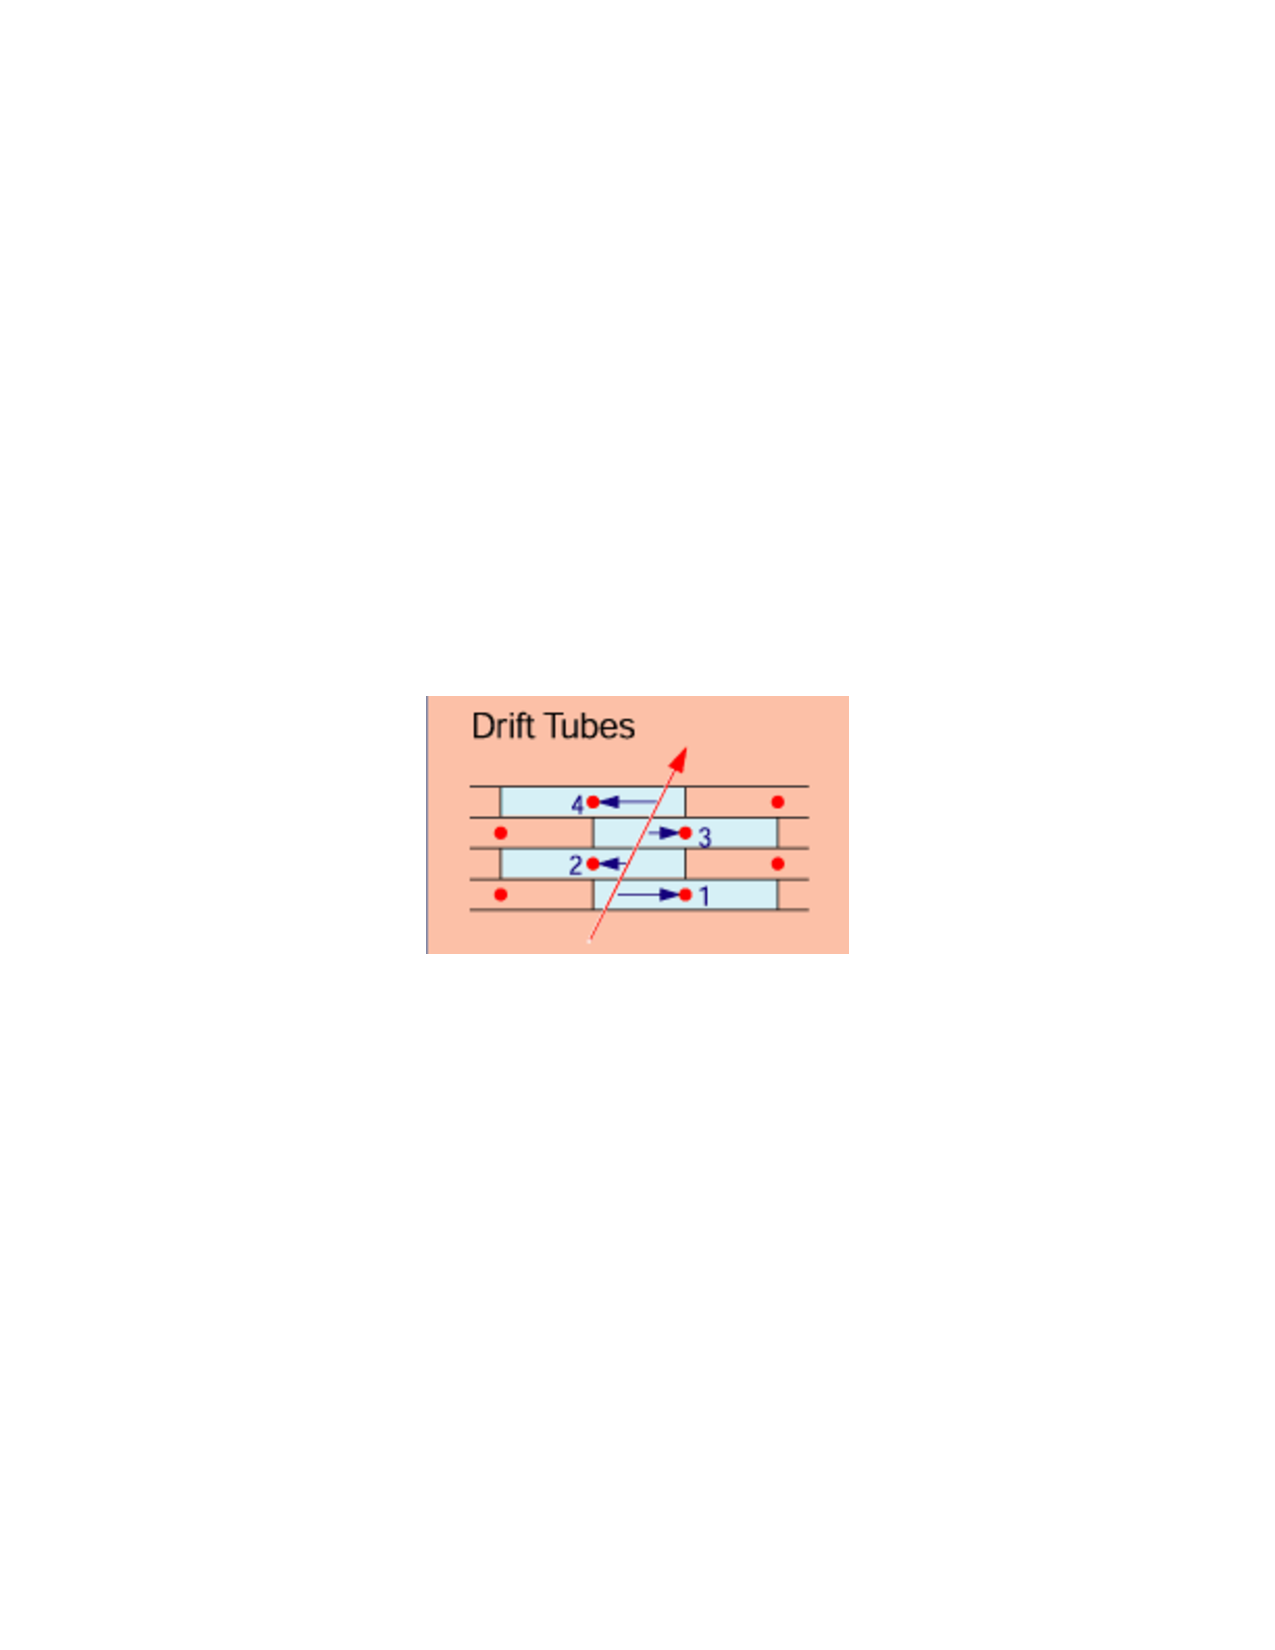
\includegraphics[width=0.8\textwidth]{cms/figs/DT.pdf}
    \caption{
      \label{fig:DT}
      A cartoon depiction of a set of drift tubes is shown in this figure
      where a charged particle passing through the system ionizes the gas,
      and the ions are collected on the wires to detect a signal.      
    }
  \end{center}
\end{figure}

There are 540 CSCs shown in figure~\ref{fig:CSC}.
The CSCs are made up of negatively charged wires (anodes) and positively charged strips (cathodes) within a gas volume.
The gas molecules within this volume are ionized when a muon passes through the volume.
This leads to a measurable hit on both the anodes and cathodes, and they are perpendicular to eachother so that the muon's trajectory can be reconstructed accurately.
There are six layers in each CSC module, which helps to accurately identify muons.

\begin{figure}[!htb]
\begin{center}
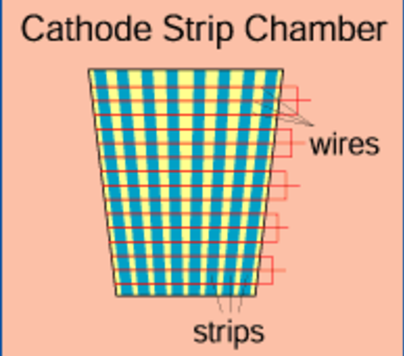
\includegraphics[width=0.8\textwidth]{cms/figs/CSC.pdf}
\caption{ A cartoon depiction of a cathode strip chamber is shown in this figure. 
\label{fig:CSC}
}
\end{center}
\end{figure}

There are 610 resistive plate chambers (RPCs), an example of which is shown in figure~\ref{fig:RPC}.
These are designed to have overlapping trigger coverage with the other components of the muon system for $\eta <$ 2.1.
Each RPC is made of two very high resistance plates, separated by a volume of gas.
They are charged kept at a high voltage and when a muon passes through the gas, electrons are knocked off of the molecules.
Metal strips are used to read out the position of the hit, and the muons momentum is measured with this information.
The readout for the RPCs is very fast (1 ns) which makes it ideal to use for triggering events with good muons.

\begin{figure}[!htb]
  \begin{center}
    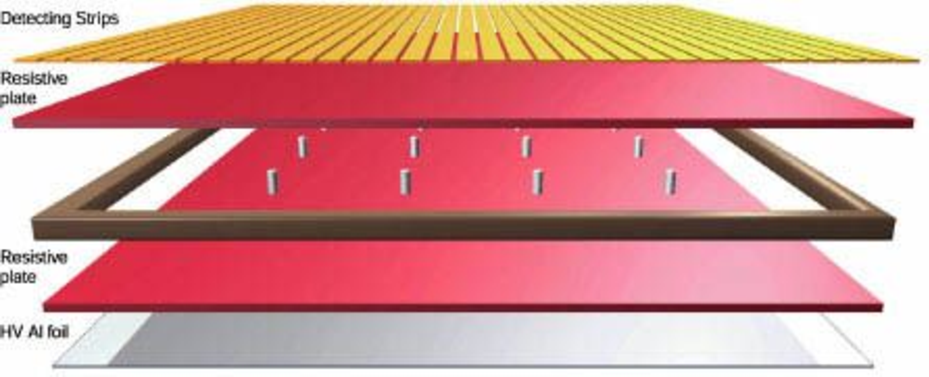
\includegraphics[width=0.8\textwidth]{cms/figs/RPClayers.pdf}
    \caption{
      \label{fig:RPC}
      A cartoon depiction of a resistive plate chamber is shown in this figure. 
    }
  \end{center}
\end{figure}

\section{Physics objects}
The data taken by the CMS detector has to be processed in such a way that all the physics processes that happen in a single collision can be reconstructed.
Each reconstructed collision is called an event.
In each event, there are multiple physics objects that are reconstructed.
The main objects that are pertinent to this analysis are electrons, muons, jets, and photons.
Each of these objects has a unique signature in the detector, but it is still possible for this signature to be faked.
The reconstruction of these objects is discussed in detail in the following sections.

\subsection{Particle Flow}
\label{subs:particleflow}
In order to classify objects, an algorithm named particle flow (PF) is used~\cite{pfReco}. 
The main goal when using the PF algorithm is to account for all energy deposits measured in the detector in a consistent fashion.
The way this is done is by clustering energy deposits measured across all subdetectors into separate PF candidates.
Once an object is classified, the clustering is done again with all the energy associated with the classified object removed.
This process is repeated until all measured energy deposits are accounted for.
For example, a charged hadron would be reconstructed by first identifying a track in the tracker.
Then a check is done to see if this track is consistent with an identified electron, or muon.
If not, all the energy that is associated with this track in the ECAL and HCAL is removed from the event,
and the track measurement is used to describe the particle.
This is done because the precision of measuring charged hadrons is much better in the tracker than in the calorimeters.
This is done iteratively for all particles in the event until there are no tracks left,
then all that remain are the neutral energy deposits.
The use of particle flow leads to greatly improved measurements of jets since more of the jet energy is measured using the tracker.
This also leads to a higher precision measurement of missing transverse energy for the same reasons.

The objects that are identified by this algorithm are listed below.
In order to further reduce fakes from contaminating our signal region, we make additional cuts to help classify objects.
These cuts are described in detail in the following section for each object we are interested in.

\begin{itemize}
\item muon          
\item photon        
\item charged hadron
\item neutral hadron
\item electron      
\end{itemize}

\subsection{Vertex Determination and Pileup}
\label{ssec:vtxandpileup}
The LHC collides protons in large bunches to maximize the probability of a hard collision.
Multiple pairs of protons interact at each bunch crossing,
and the number of interactions is stochastic but depends on the beam intensity.
Each proton proton collision can produce particles that get reconstructed,
and when these particles are reconstructed they are associated to a specific proton proton collision using charged particle information.
It is important to identify which proton-pair interaction is responsible for triggering the event being studied.
Every particle track is associated with a unique vertex,
and the primary vertex is chosen by finding the vertex with the largest sum of $\mathrm{(p_{T})^{2}}$ of tracks associated with that vertex.
Neutral candidates do not have associated tracks, so they are defined to always be from the primary vertex.
The energy of objects affected by this reassociation is recalibrated, and this calibration is described in section~\ref{ssec:jets}.

Pileup is defined as energy in the detector which does not come from the primary collision or primary interaction.
There are two primary sources of pileup, in-time pileup (ITPU), and out-of-time pileup (OOTPU).
ITPU occurs when protons other than those in the primary interaction interact in the same bunch crossing,
and the particles produced are reconstructed.
OOTPU occurs mainly due to the fact that protons are collided with a frequency of 25ns,
and the timing resolution of some detector components is not fast enough to resolve which bunch crossing certain reconstructed particles came from.
The number of expected pileup events can be determined using equation~\ref{eqn:pileup} where$\mathcal{L}_{inst.}$ is the instantaneous luminosity,
$\sigma(p-p)_{inelastic}$ is the total inelastic scattering cross section for protons,
and $f_{collision}$ is the collision frequency.
For 2015, this value is 12.75.

\begin{equation}
\label{eqn:pileup}
  \mathrm{N_{pileup} = \mathcal{L}_{inst.}*\sigma(p-p)_{inelastic}*f_{collision}}
\end{equation}

All of the energy from pileup comes from proton-proton interactions other than the primary interaction.
These ``soft'' interactions produce predominantly hadronic final states,
and the majority of these interactions are due to gluons scattering off of quarks or other gluons.
These final states inherently do not have \MET\ due to particles escaping detection due to them being hadronic,
and this leads to a balance in the overall energy deposited in the detector.
There are still contributions to \MET\ from to pileup due to the poor resolution of jets in CMS.
A calibration is applied to account for pileup according to the method described in section~\ref{sec:t1met}.


\subsection{Isolation}
\label{ssec:isolation_summary}
Isolation is a concept that is very important when identifying leptons, and photons.
Isolation can be simply described as the total energy in the detector near an object of interest.
When leptons or photons from the primary interaction are not produced together with colored objects,
they are deemed prompt.
Non-prompt leptons, such as those from a b-quark decaying semi-leptonically,
and non-prompt photons such as those from $\pi ^{0}$ decay,
are always produced in conjunction with a hadronic shower.
These non-prompt objects are then very likely to be non-isolated due to the hadronic energy nearby.
The distance between two objects ($\Delta$R) is defined by equation~\ref{eqn:DR},
where $\phi$ is the angle measured in plane transverse to the beam direction,
and $\eta$ is the psuedorapidity defined by equation~\ref{eqn:psuedorapidity}.
In the equation for $\eta$, the variable $\theta$ is defined as the angle measured from the beam axis to the axis of the transverse plane to the beam axis.
In particle physics, $\eta$ is preferred over $\theta$ when describing a particle's momentum along the beam axis because changes in $\eta$ are lorentz invariant,
whereas the same is not true for changes in $\theta$.

\begin{equation}
  \label{eqn:DR}
  \Delta R = \sqrt{\Delta\eta^{2}+\Delta\phi^{2}}
\end{equation}

\begin{equation}
  \label{eqn:psuedorapidity}
  \eta = -\ln(\mathrm{tan}(\frac{\theta}{2}))
\end{equation}

The choice of what to include when calculating isolation is defined differently for each object and will be described in the following sections.

\subsection{leptons and photons}
\label{ssec:lepsandphots}
Z bosons decay leptonically to $e\bar{e}$, $\mu\bar{\mu}$, and $\tau\bar{\tau}$~pairs 3.363 $\pm$ 0.004\%, 3.366 $\pm$ 0.007\%\ and 3.370 $\pm$ 0.008\% of the time respectively.
The rest of the time they decay to neutrinos, or to quark-antiquark pairs.
This analysis focuses on decays to $e\bar{e}$ and $\mu\bar{\mu}$.
This is due to the fact that $\tau$s have a large mass and short lifetime which leads to them decaying.
This is further complicated by the fact that $\tau$s decay to an electron ($\mu$) and two neutrinos 17.85 $\pm$ 0.05\% (17.36 $\pm$ 0.05\%) of the time,
and the rest of the time the $\tau$ decays to hadronic final state particles.
This leads to worse measurements in leptonic final states due to the missing energy from not detecting the neutrinos,
and makes it hard to distinguish $\tau$s from jets in hadronic channels.
In order to keep the analysis simple, this search is done in final states with $Z\rightarrow ee$ and $Z\rightarrow\mu\bar{\mu}$ only,
and when referencing leptons, only electrons and muons are considered.
It is also important to be able to identify photons in order to measure one of the main backgrounds.

The depth of the ECAL is \textasciitilde{}25 radiation lengths which means electrons and photons lose almost all of their energy in the ECAL.
Another thing that helps to distinguish electrons from photons is that electrons will deposit energy in the silicon tracker whereas photons will not.
Therefore, a track can be matched to energy deposits in the ECAL to help identify electrons.
Similarly, a track found to correspond to a hit in the ECAL can be used to help determined that the energy deposited in the ECAL was not from a photon.

A different approach is taken to identify and measure muons in the CMS detector.
Since muons are charged, they leave hits in the silicon detector which can be reconstructed as a track.
The ECAL and HCAL are designed to contain all measureable energy,
but due to the minimum ionizing nature of muons, muons are able to pass through these subdetectors without depositing much energy.
The muon subdetector is the outermost layer of the CMS detector, and it is designed to identify muons.
Muon tracks can be measured independently in the muon subdetector,
and the measurement is matched to a set of hits in the tracker to determine the final muon energy.

The main thing all of these objects have in common is they are produced in interactions that do not have a hadronic component.
Quantifying this energy is done by calculating the particles isolation, as described in section~\ref{ssec:isolation_summary},
and is used to discriminate against unwanted physics processes.



\subsection{jets}
\label{ssec:jets}
A jet is an object used to represent a single parton, and it can be simply described as a substantial amount of hadronic activity concentrated in a single region of the detector.
The region is defined using the ``anti-$\mathrm{k_{T}}$'' (ak) algorithm~\cite{antikt} with a jet radius of 0.4.
For jets in this analysis, the charged candidates not associated with the primary vertex are removed before clustering. 
This removes some unwanted energy from pileup, and the jets are then calibrated in order to more accurately reflect the energy of the particles they represent.

The jet energy corrections are done in multiple levels, labeled as L1,L2 and L3.
A detailed procedure of how the corrections are applied can be found here~\cite{CMS-DP-2015-044}.
Jets are corrected such that the calibrated energy is as close as possible to the parton that produced the jet.
The corrections are derived using MC, and each level corrects for different effects in the following way:
L1 corrects for pileup,
L2 corrects for different responses in the detector as a function of $\eta$,
and L3 corrects the overall energy scale.
The L1 correction is done by assuming a flat overall energy density from pileup in the detector which is calculated per event,
and then subtracting this energy from the jet using the jet area to determine the overall energy contributed from pileup.
The L2 correction is done by selecting di-jet events where one of the jets is central($\eta < 0.8$) and the second jet is non-central ($\eta > 0.8$).
Scale factors are then derived to correct the energy measurement for the non-central jet in separate regions of $\eta$.
The L3 correction is done by deriving scale factors as a function of jet \pt\ which correct the jet energy to match the true energy of the parton that the jet came from.

In addition to the L1, L2 and L3 corrections, residual corrections are derived in data control regions to correct for differences in the detector response to jets between data and MC.
This is done in a region with at least one photon or a Z boson which decays to two leptons, where the boson recoils off of a jet.
The photon and leptons are measured with better resolution than the jets, so scale factors are derived as a function of \pt\ to correct the detector response of jets.
The full description of cuts used to define jets for the analysis is defined in sub-section~\ref{ssec:jetsel}.

This is to acknowledge all the other members of the CMS experiment who made it possible to produce
the figures and tables appearing in this chapter.

% --------------------------------------------------------------------------- %
% --------------------------------------------------------------------------- %
\chapter{Missing Transverse Momentum}
\label{ch:MET}
% --------------------------------------------------------------------------- %
% --------------------------------------------------------------------------- %
In the final state targeted by this analysis, a gravitino is proposed as the LSP.
This particle is weakly interacting and makes a good dark matter candidate
which lead to signal events having large values of \MET\ due to this particle escaping detection.
It is important that \MET\ from standard model processes is predicted accurately.
\MET\ can be calculated using the full collection of PF candidates described in section~\ref{subs:particleflow}.
In the following sections, \MET\ calculations and corrections are described in detail.

\section{raw \texorpdfstring{\MET}{MET}}

Calculating \MET\ using PF candidates is done by summing the transverse momentum vectors of all the PF candidates, described in equation~\ref{eqn:rawmet}.

\begin{equation}
  \label{eqn:rawmet}
\mathrm{\overrightarrow{E_{T}^{miss}} = -\sum_{i}\overrightarrow{p}_{T}^{i}}
\end{equation}

When \MET\ is calculated without any calibration applied to the pf candidates, it is known as raw MET.

\subsection{Sources of \texorpdfstring{\MET}{MET}}
\label{sec:metsources}
\MET\ comes from three main sources,
noise in the detector from various sources,
resolution effects due to mismeasurement of physics objects and
visible particles from the hard interaction being too far forward in $\eta$ to be within the detector geometry (referred to as fake \MET)
and particles from real physics processes not interacting with the detector thereby escaping detection.

\MET\ due to noise in the detector can lead to huge tails in the \MET\ distribution.
The size of this effect is shown in figure~\ref{fig:cleanmet} for the data taken in 2012.
A set of filters is applied to mitigate these effects,
and the details of these filters is described in section~\ref{ssec:metfilter}.

\begin{figure}[!ht]
  \begin{center}
    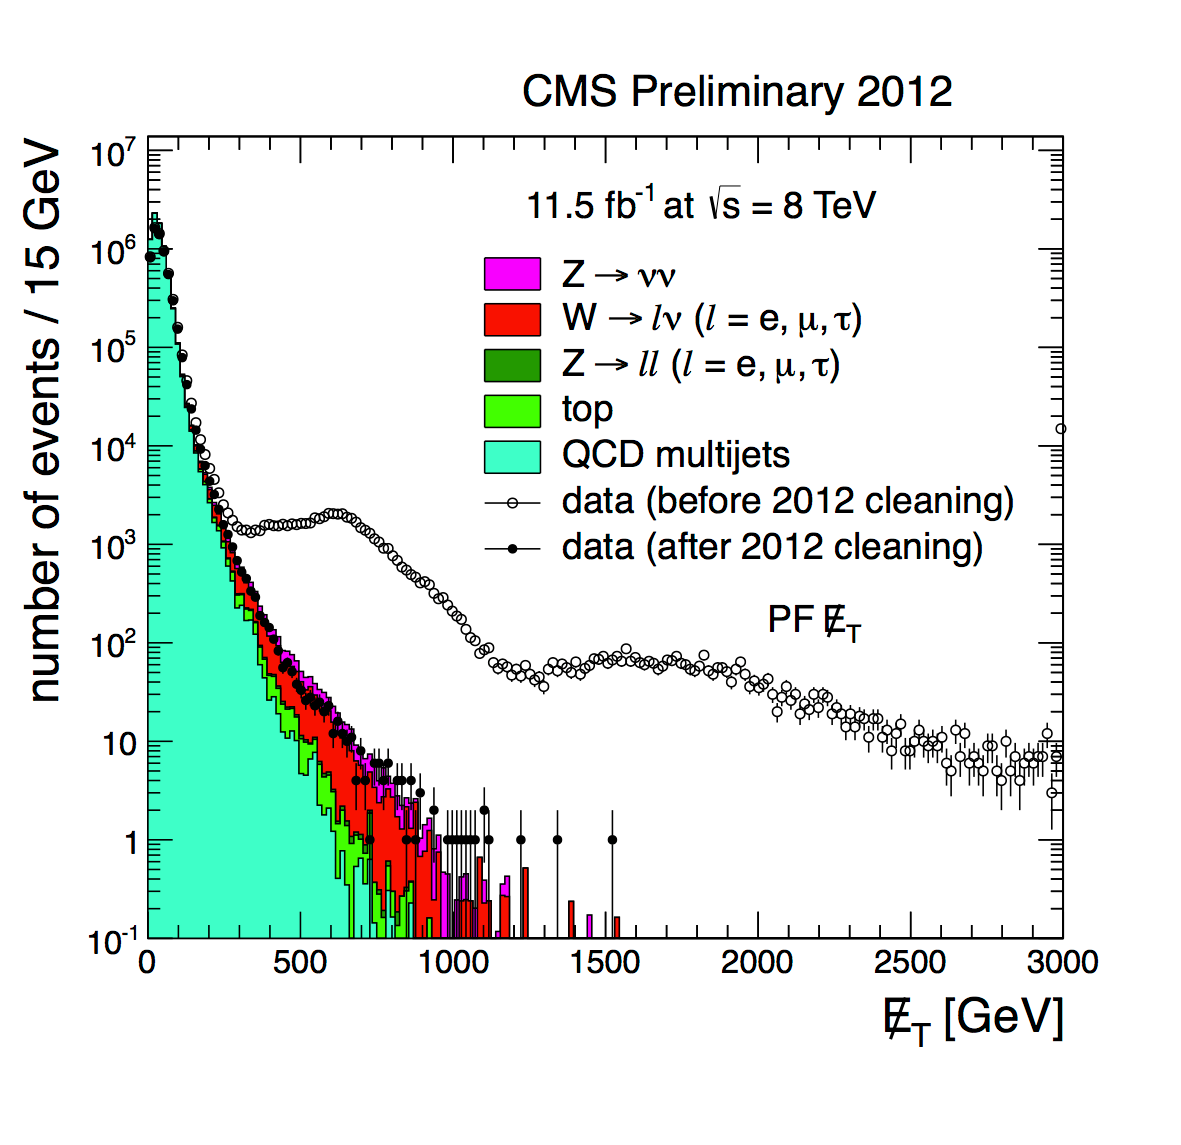
\includegraphics[width=0.8\textwidth]{MET/figs/Fig4EventCleaning.pdf}
    \caption{
      \label{fig:cleanmet}
      \MET\ distributions for events passing the dijet selection without 2012 cleaning algorithms applied (open markers),
      with 2012 cleaning algorithms applied including the one based on jet identification requirements (filled markers),
      and events from MC (filled histograms).
    }
  \end{center}
\end{figure}

Particles that do not interact with the detector that lead to real \MET\ can be standard model neutrinos, or particles from BSM theories such as the $\mathrm{\tilde{G}}$.
Since this analysis is searching in regions with large \MET, it is very important to be able to identify and measure backgrounds with fake \MET and real \MET.

\section{Type-1 \texorpdfstring{\MET}{MET}}
\label{sec:t1met}
In order to reconstruct \MET\ with high precision, corrections that are made to physics objects need to be propagated to the \MET\ variable.
The corrections with the largest impact on the \MET\ resolution are the jet corrections, since jets have the worst resolution.
Energy from pileup in each event is deposited randomly in the detector, and is expected to be balanced.
It can happen that some pileup energy deposited overlaps with energy from a jet coming from the hard interaction.
A correction is applied to the jet to account for this effect,
however if the pileup energy removed from each jet's cone were to be propagated to the \MET, it would create an imbalance.
This is taken care of by adding the pileup energy back in, and the overall correction to \MET\ is called the Type 1 correction.

Type 1 \MET\ refers to a version of \MET\ where the corrections that are applied to jets are propagated to the \MET\ calculation as described in section~\ref{ssec:jets}.
The correction factors applied to the jets are derived for jets down to 10 \gev.
The way these corrections are propagated to the \MET\ is not as straightforward as just adding the corrections vectorially with the \MET.

The jets we use in this analysis are made using all the pf candidates, except the charged pf candidates that are not associated with the primary vertex.
Leptons and photons are included in the collection of pf candidates used when clustering jets.
The jet corrections are meant to correct jets that come from hadronic objects, such as quarks and gluons.
If the jet corrections are applied to lepton and photon objects, the
The jet corrections are not meant to be applied to lepton and photon objects.
When propagating the jet corrections to the \MET, we exclude corrections on jets with an electromagnetic fraction larger than 90\%,
and remove the pf muon candidates from the jet when deriving the corrections.
This effectively removes photons and leptons from the objects that get corrected.

\subsection{Data vs. MC Comparison}
\label{subs:MET_datavsmc}
It is important to understand how well \MET\ is simulated in MC in order to validate the MC samples used to simulate signal and certain background predictions.
Studies were done to check the agreement in data vs. MC in different detector subsystems.
The studied region is defined simply by having at least two leptons coming from a Z boson, so no real \MET\ is expected in these events.
The \MET\ components are studied separately in different detector subsystems by choosing several categories of pf candidate type and $\eta$ region defined in table~\ref{tab:subdetector_eta}.
Charged candidates in the region with $\eta < 2.4$, can be used to study the tracker,
neutral hadronic candidates can be used to study the HCAL,
and neutral electromagnetic candidates can be used to study the ECAL.
The \MET in each region is defined by calculating the negative magnitude of the vector-sum of only the charged, neutral hadronic, or neutral electromagnetic PF candidates.
The plots showing the agreement for each \MET\ component are shown in figures~\ref{fig:chpfcands},~\ref{fig:phpfcands}, and~\ref{fig:nupfcands} respectively. 
The charged  component of \MET\ shows reasonable agreement over the entire CMS detector.
The neutral electromagnetic component of \MET\ shows good agreement in the tracker volume of CMS, and the agreement is bad for cadidates outside of the tracker.
The neutral hadronic component of \MET\ shows poor agreement in the tracker volume of CMS, and the agreement gets much worse for cadidates in the very forward region.

\begin{table}[htb]
\scriptsize
\begin{center}
\caption{
Definitions for the $\eta$ region chosen to define each subdetector region are listed in this table.
\label{tab:subdetector_eta}}
\begin{tabular}{l|c}

\hline
Subdetector Region     & $\eta$ cut \\
\hline
Barrel                 & $|\eta| < 1.3$ \\
Transition region      & $1.3 < |\eta| < 1.6$ \\
Endcap with tracker    & $1.6 < |\eta| < 2.4$ \\
Endcap without tracker & $2.4 < |\eta| < 3.0$ \\
HF region              & $|\eta| > 3.0$ \\
\hline
\end{tabular}
\end{center}
\end{table}


\begin{figure}[!ht]
\begin{center}
\begin{tabular}{cc}
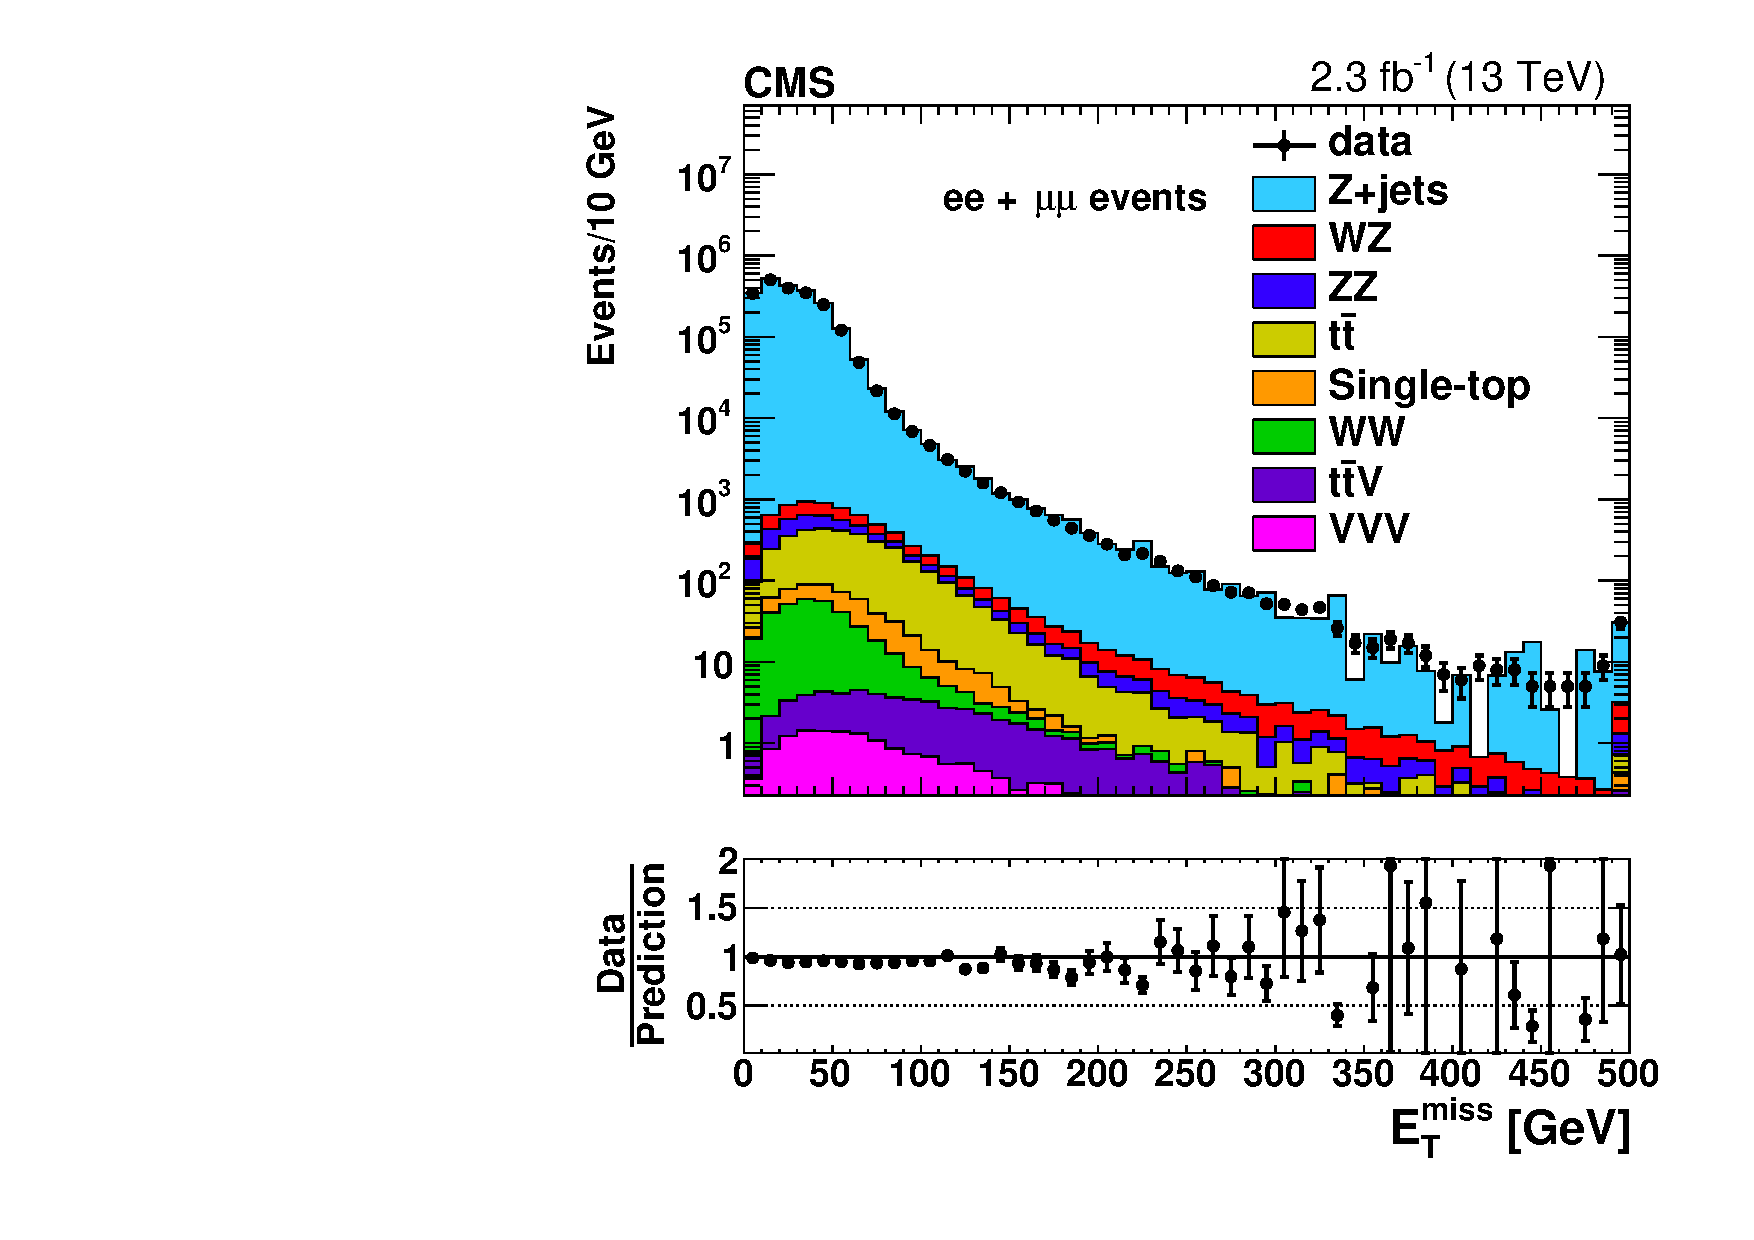
\includegraphics[width=0.4\textwidth]{MET/figs/h_met_chpfcands_0013_pt_ll_signalregion_inclusive_passtrig.pdf} &
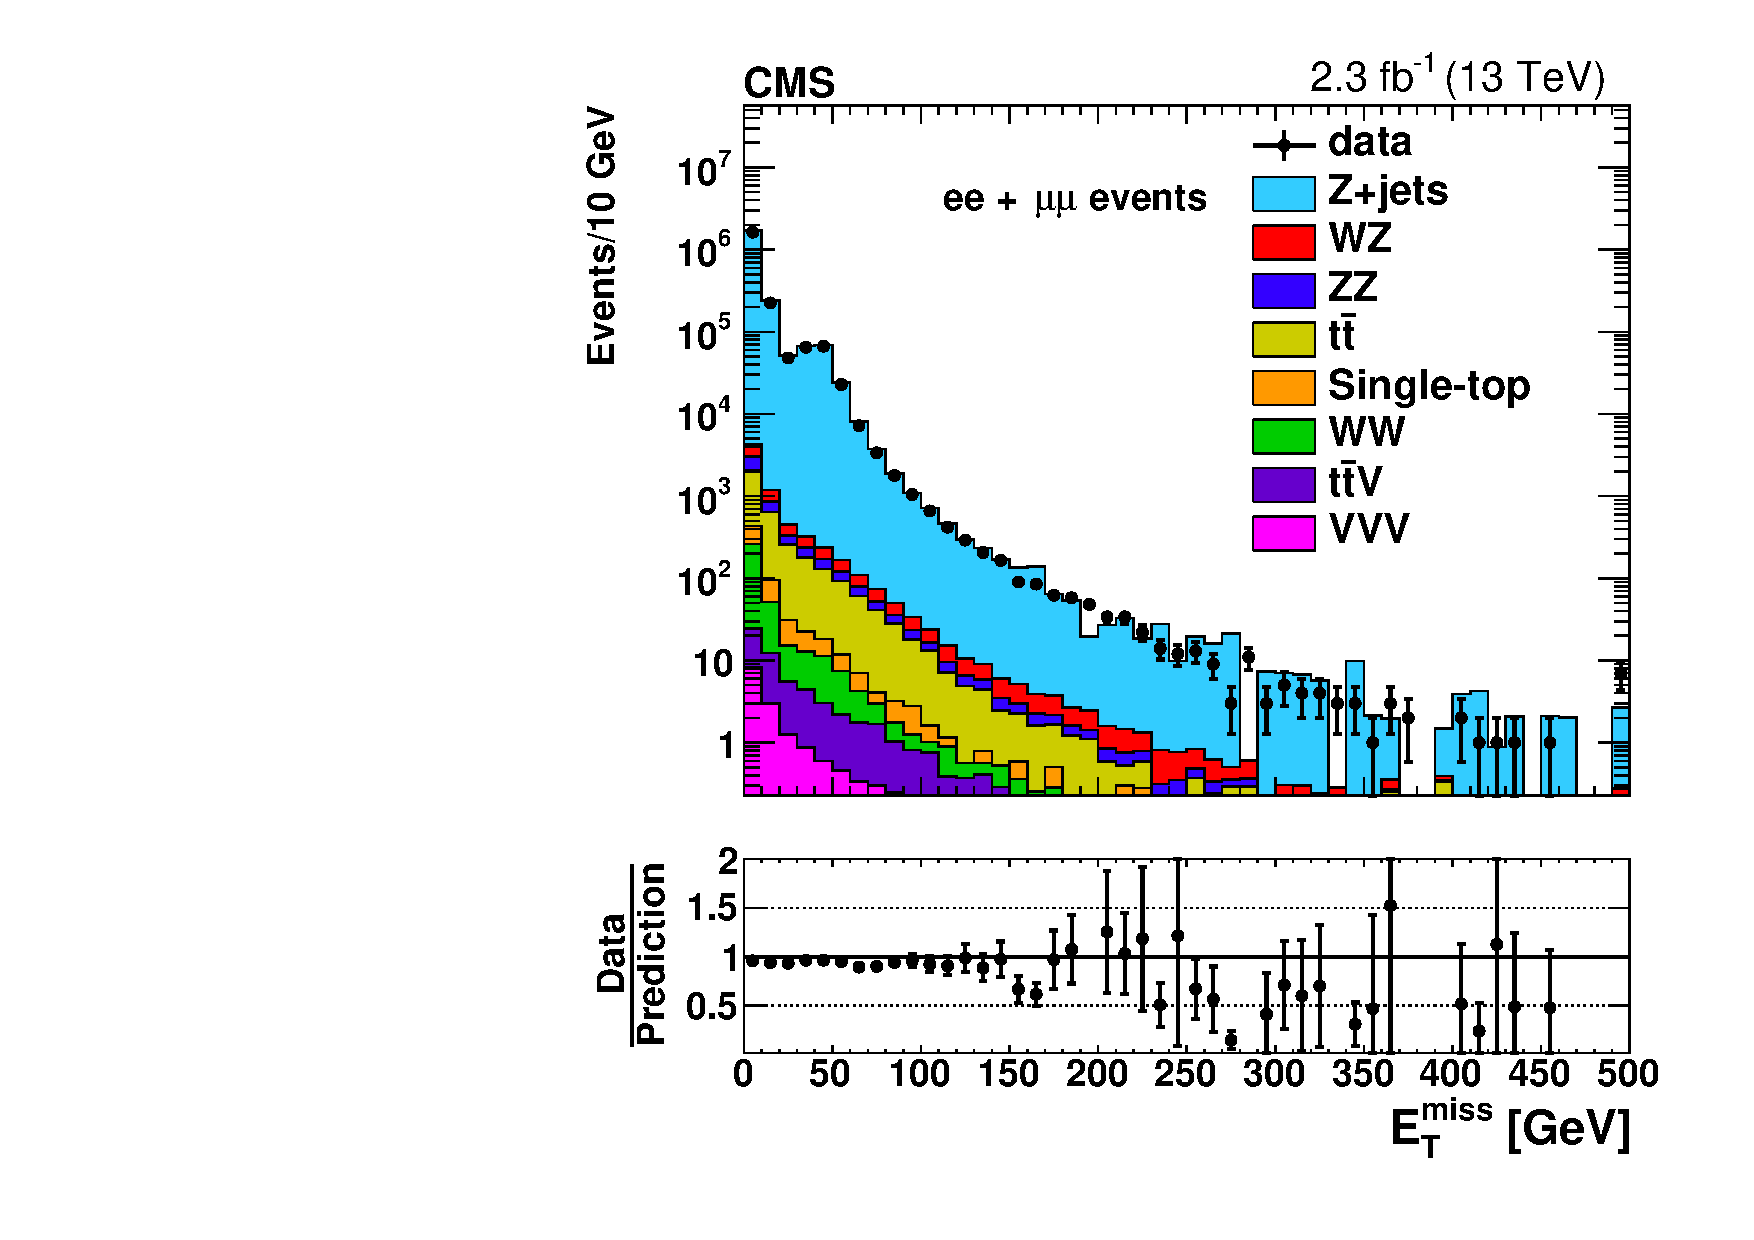
\includegraphics[width=0.4\textwidth]{MET/figs/h_met_chpfcands_1316_pt_ll_signalregion_inclusive_passtrig.pdf} \\
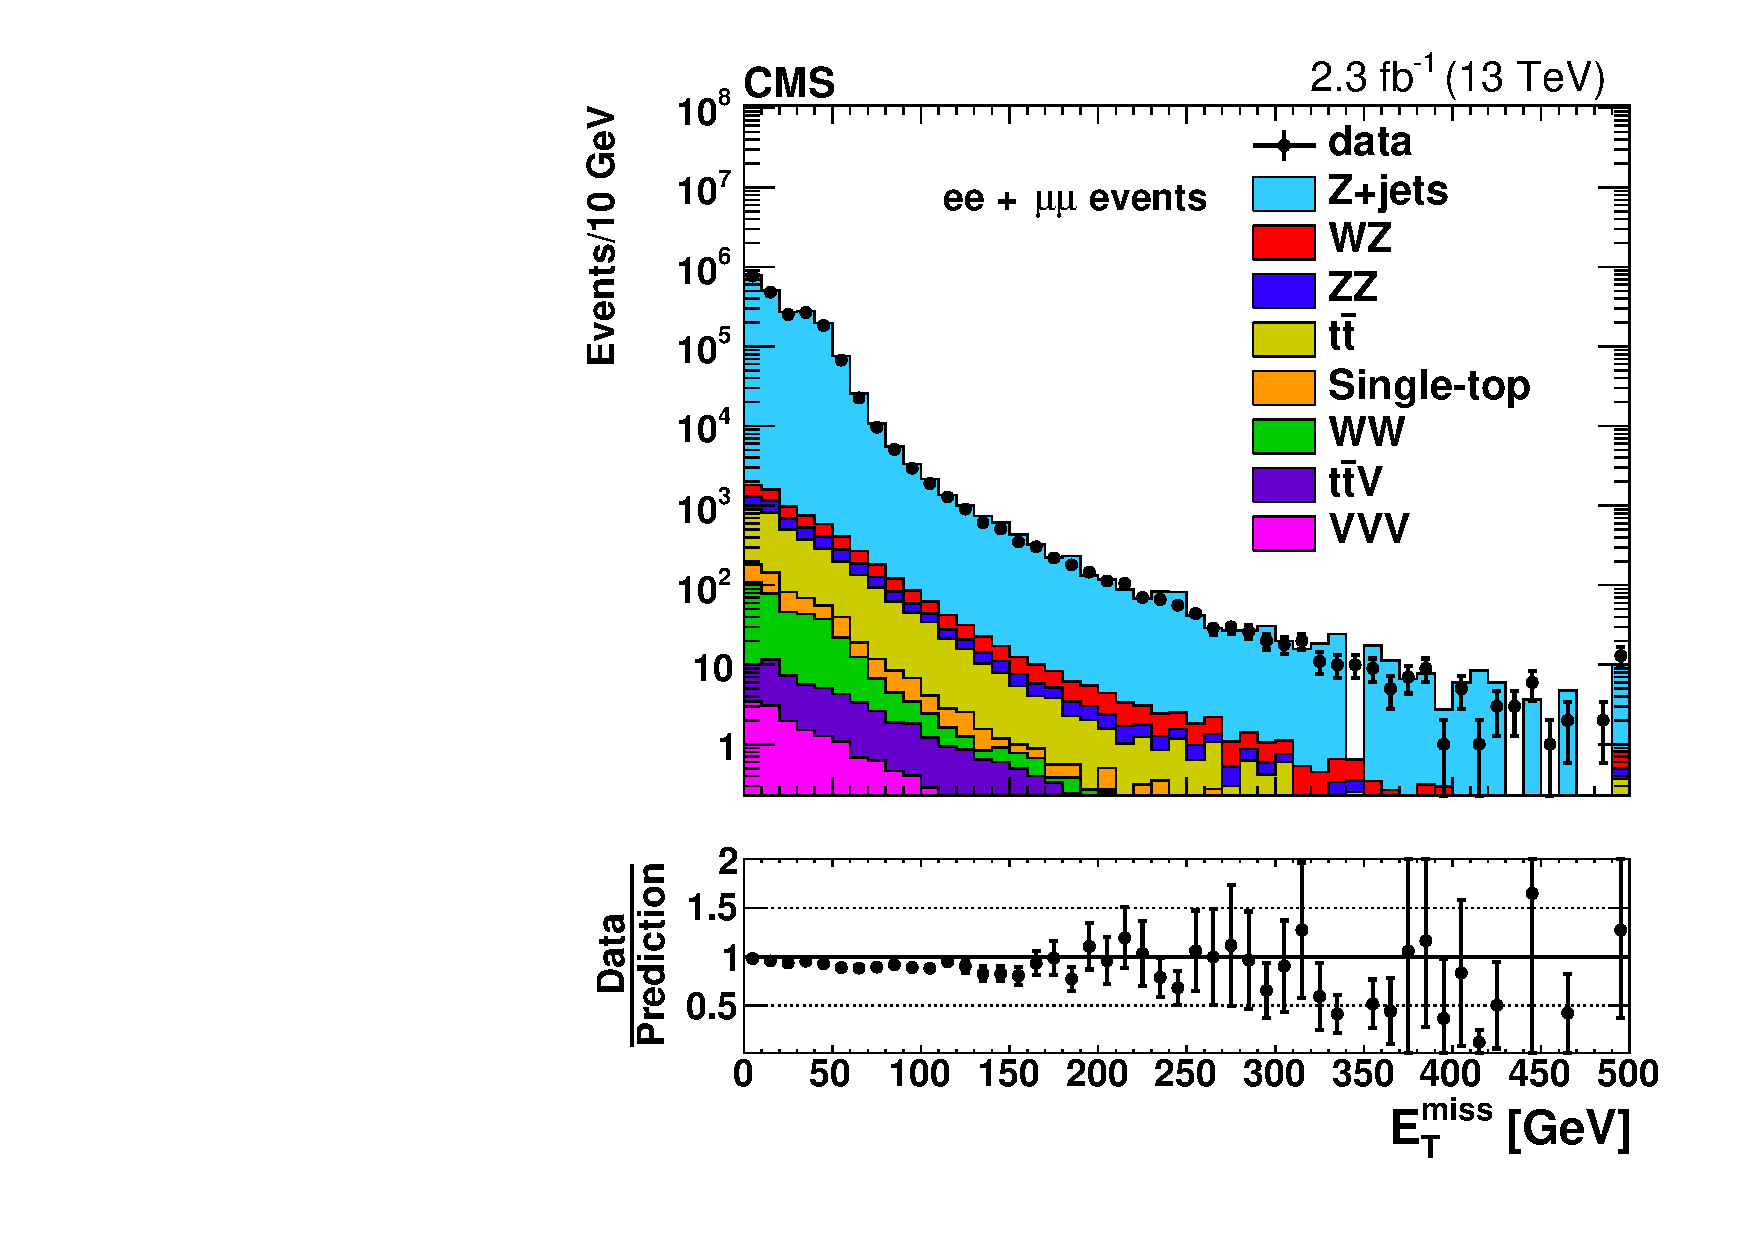
\includegraphics[width=0.4\textwidth]{MET/figs/h_met_chpfcands_1624_pt_ll_signalregion_inclusive_passtrig.pdf} &
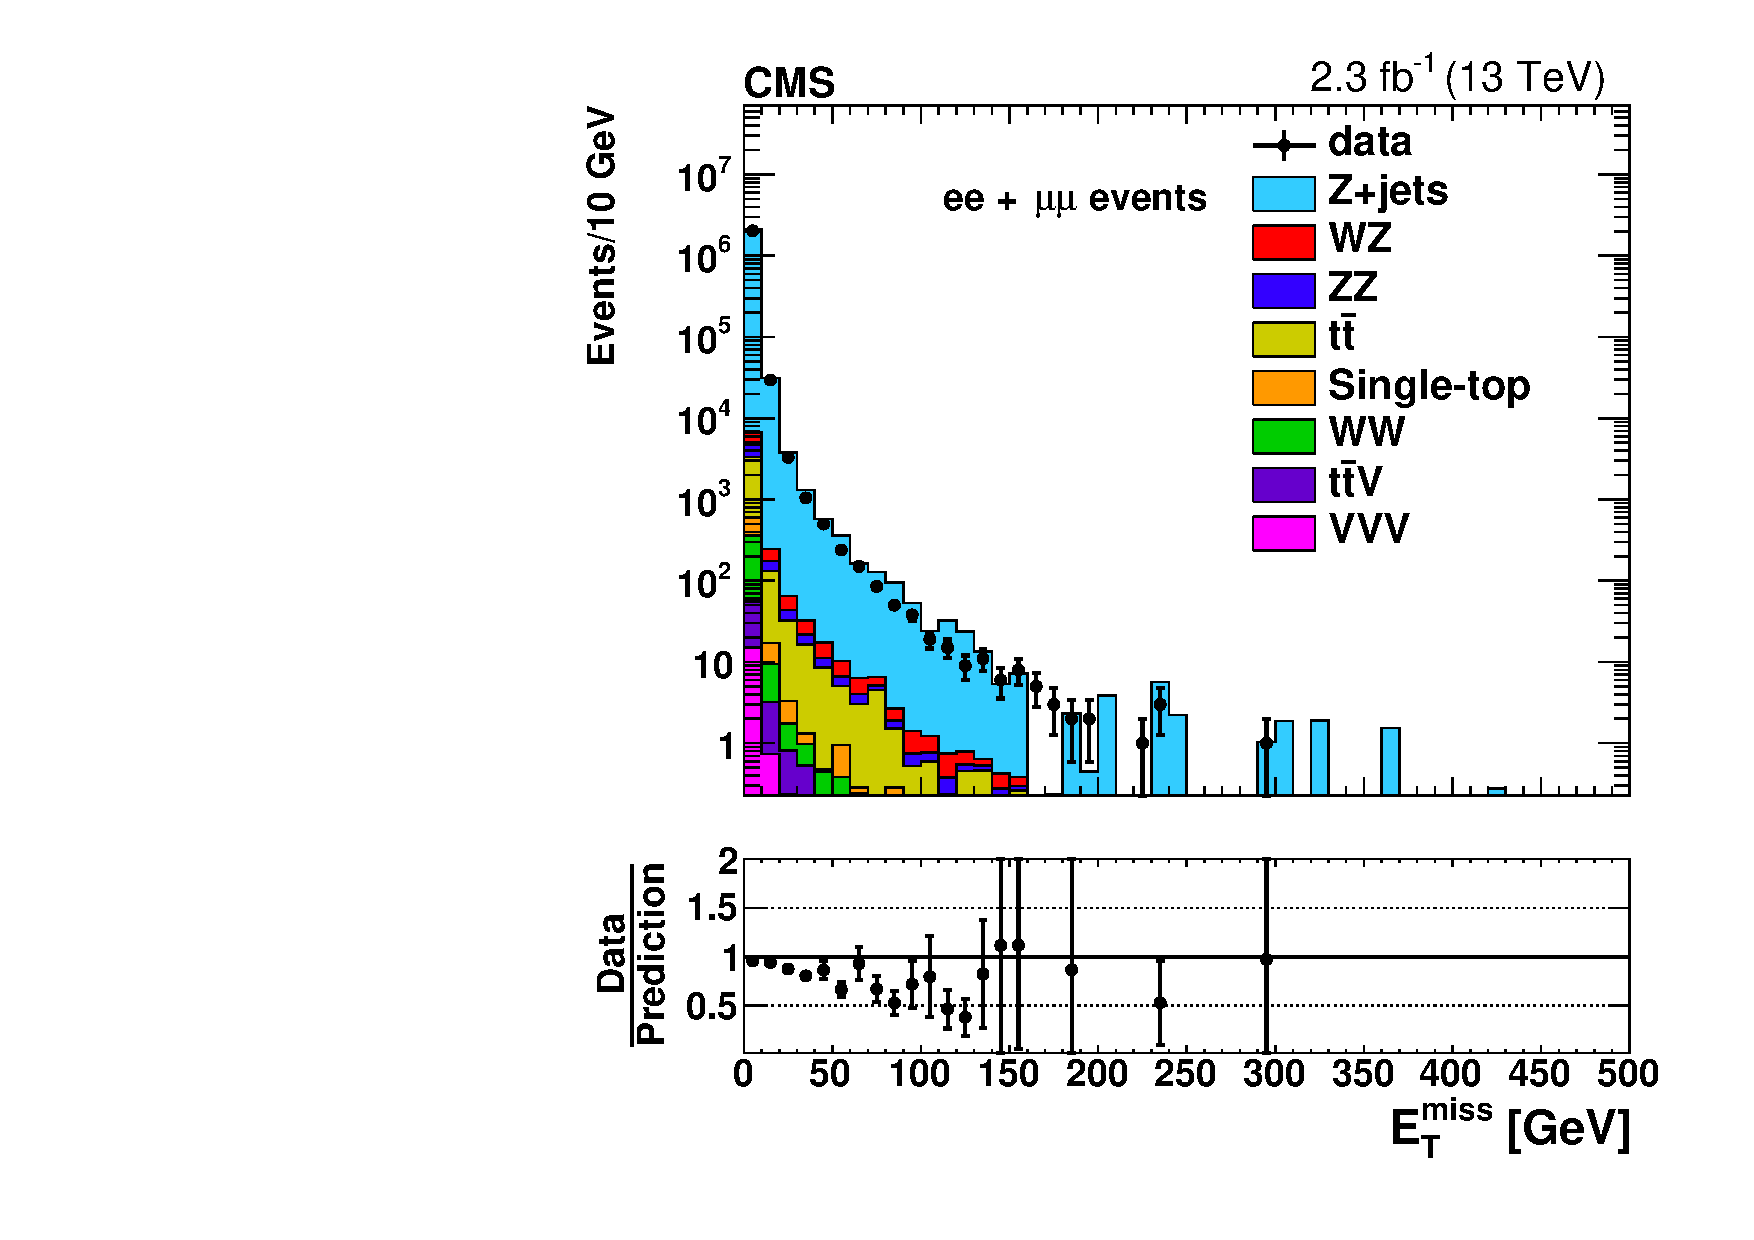
\includegraphics[width=0.4\textwidth]{MET/figs/h_met_chpfcands_2430_pt_ll_signalregion_inclusive_passtrig.pdf} \\
\end{tabular}
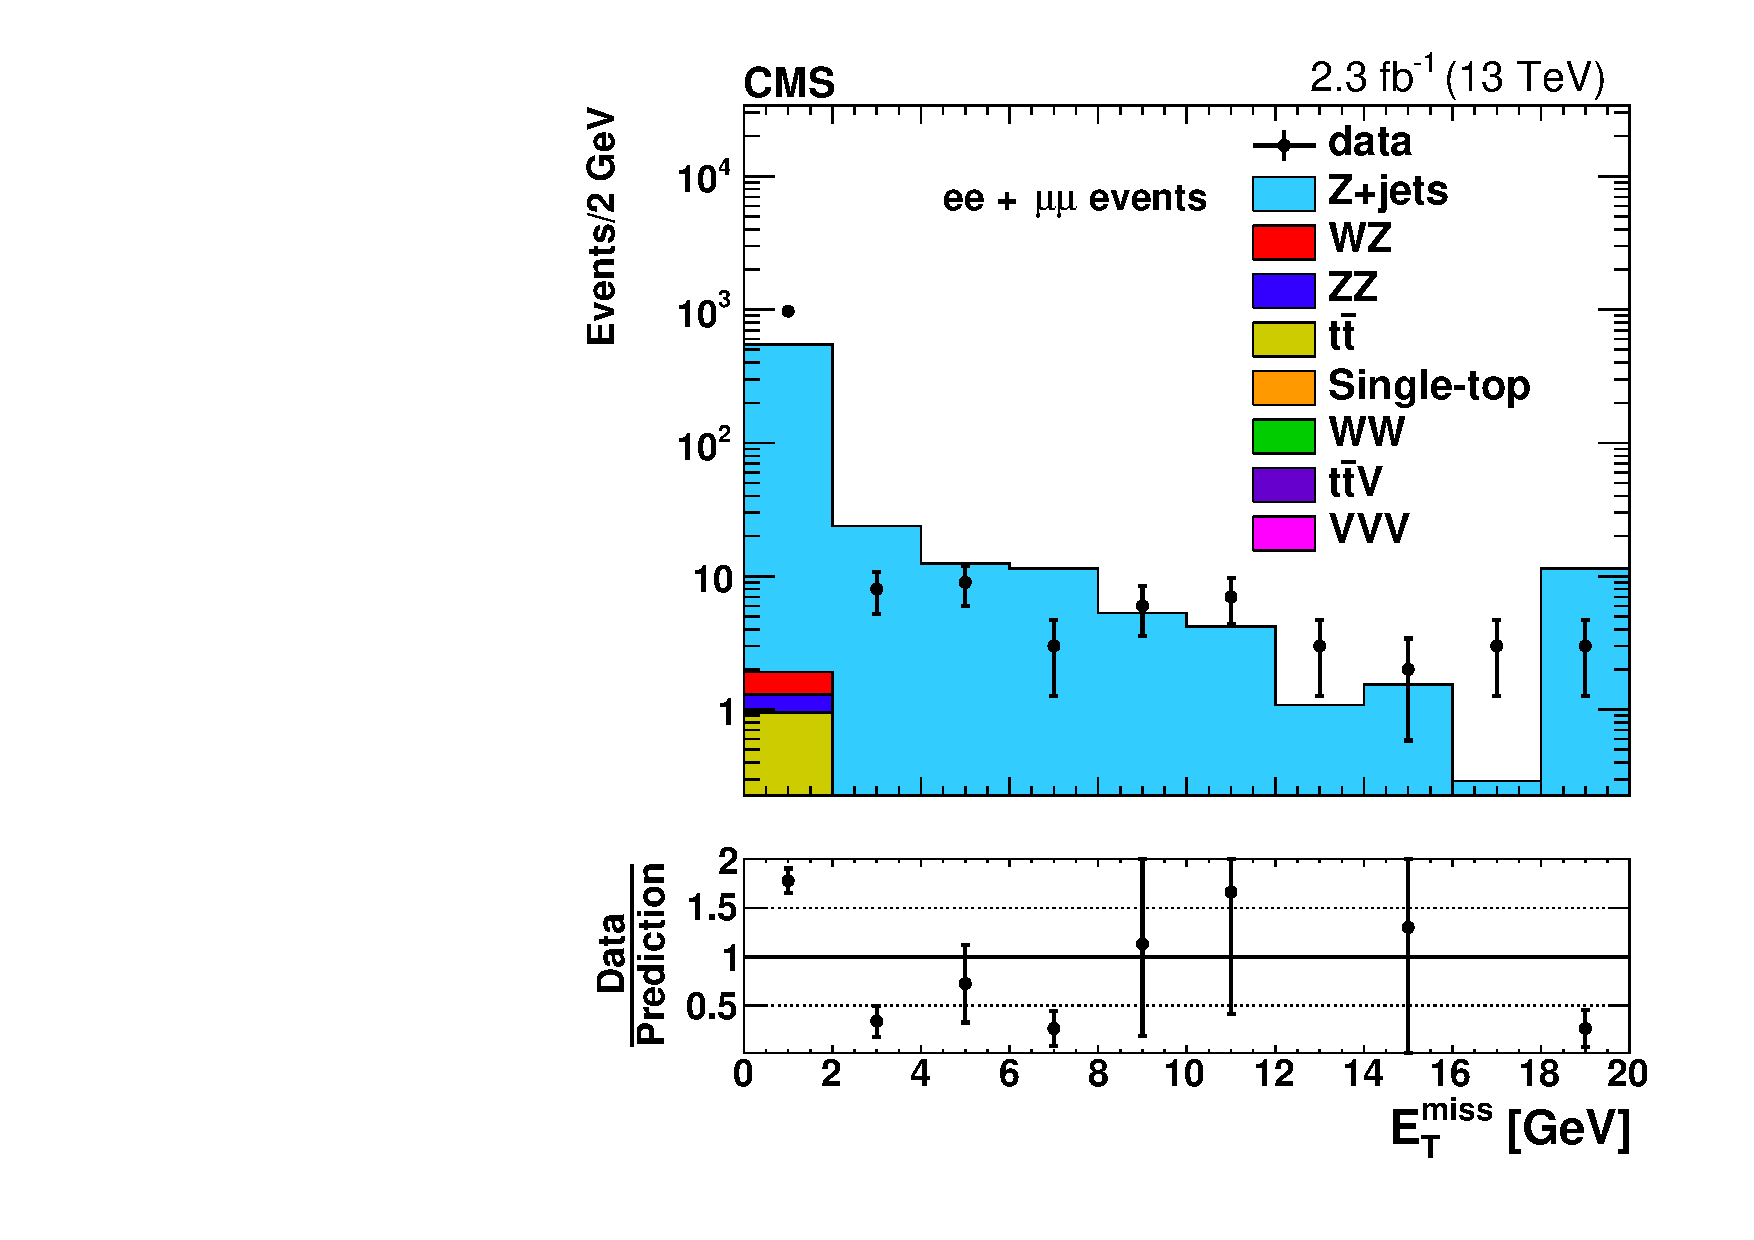
\includegraphics[width=0.4\textwidth]{MET/figs/h_met_chpfcands_30in_pt_ll_signalregion_inclusive_passtrig.pdf} 
\caption{The \MET\ distribution is shown for charged PF candidates only.
The top row shows the barrel region on the left and transition region between the barrel and endcap on the right,
the second row shows the endcap region including the tracker on the left and endcap region excluding the tracker on the right
and the bottom row shows the HF region only.
\label{fig:chpfcands}
}
\end{center}
\end{figure}

\begin{figure}[!ht]
  \begin{center}
    \begin{tabular}{cc}
      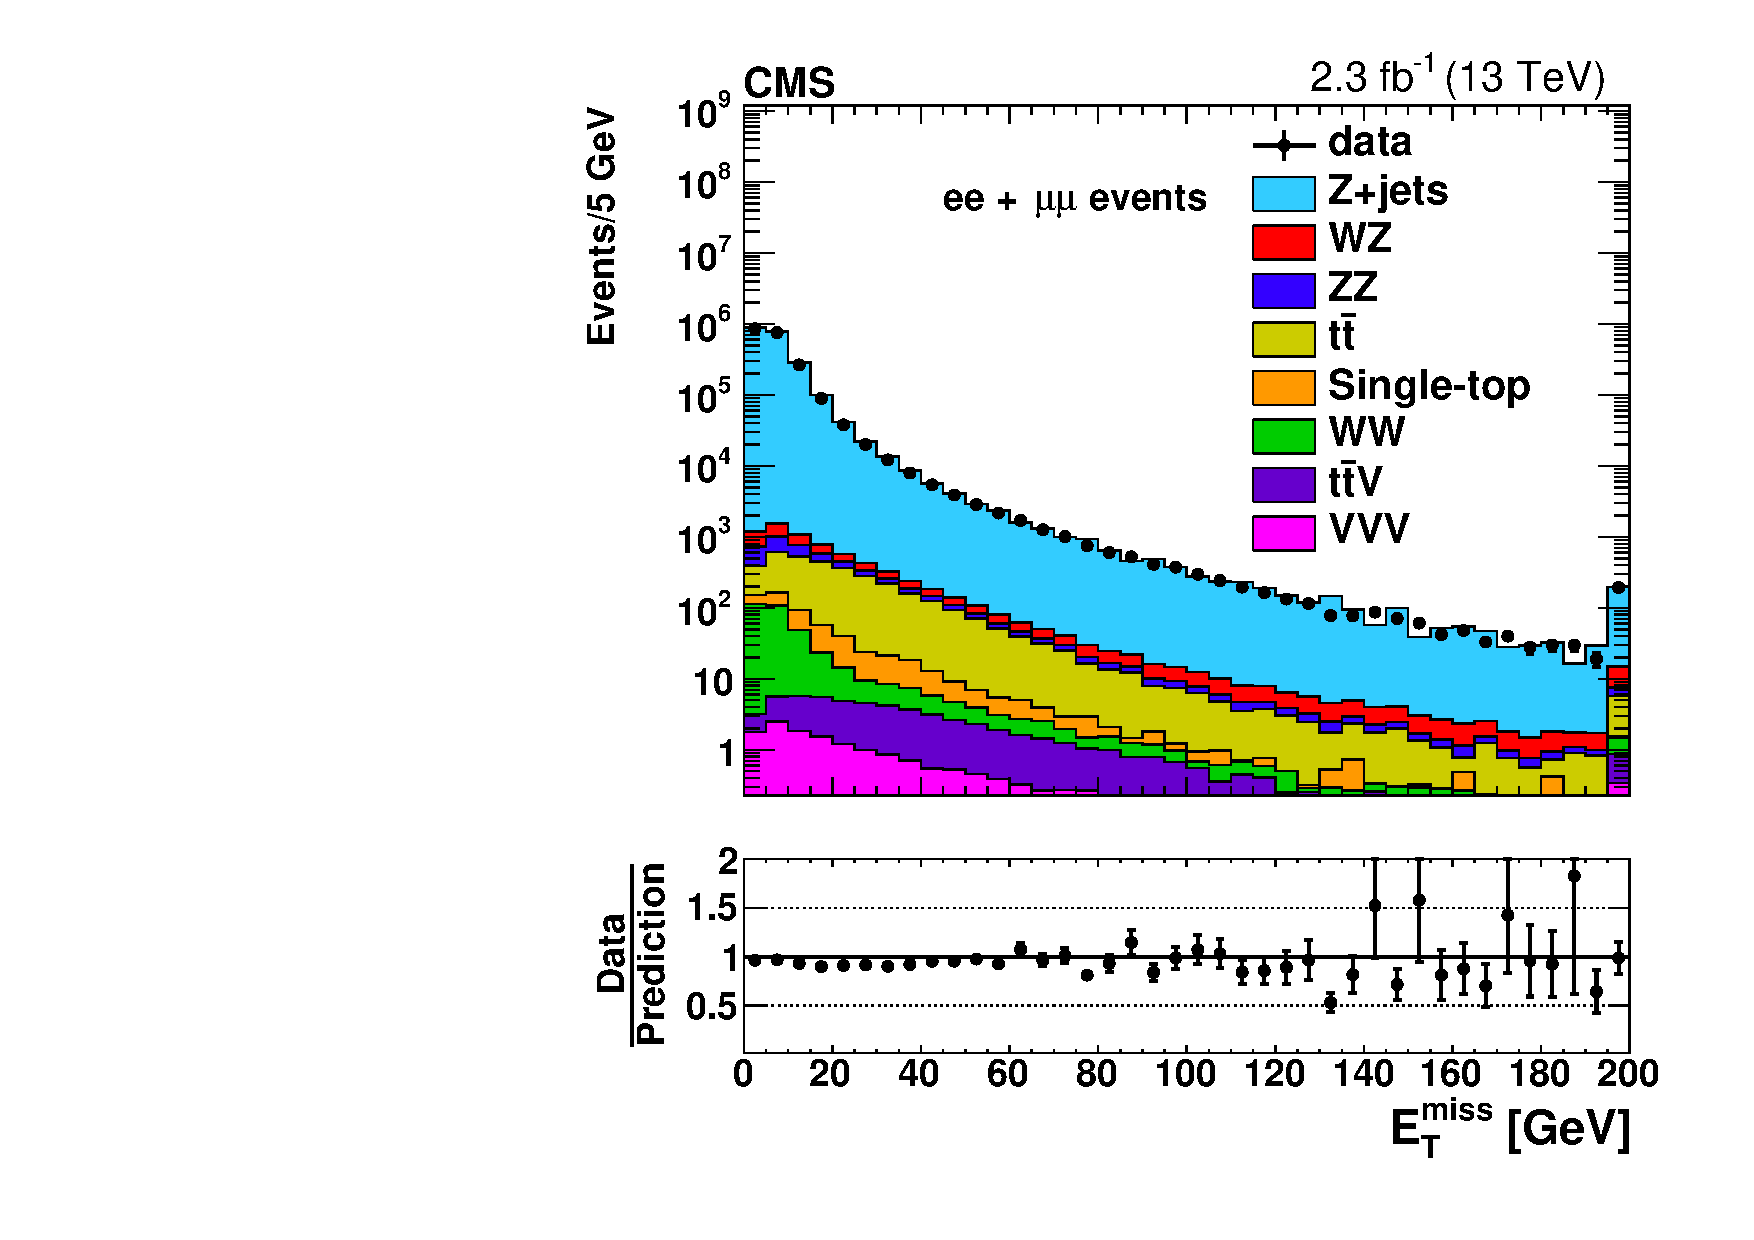
\includegraphics[width=0.4\textwidth]{MET/figs/h_met_phpfcands_0013_pt_ll_signalregion_inclusive_passtrig.pdf} &
      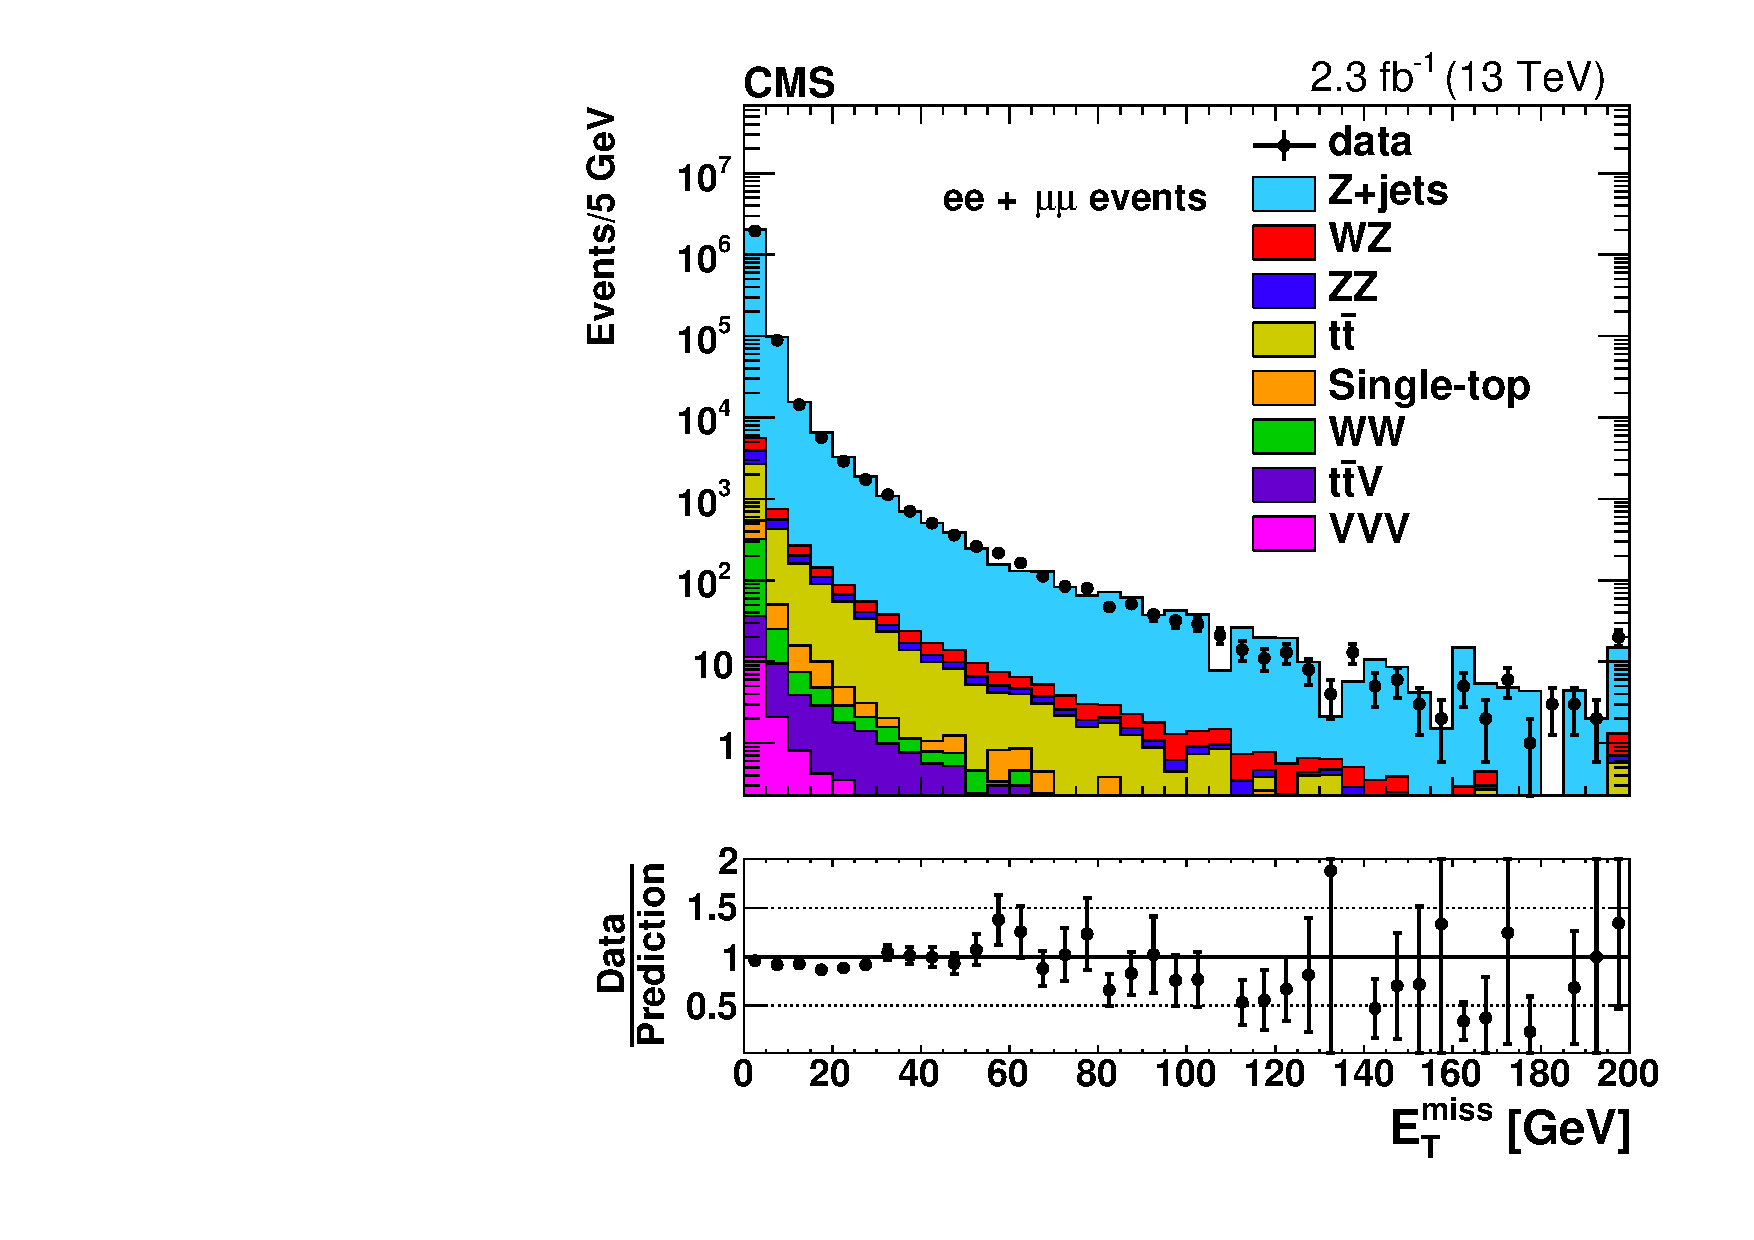
\includegraphics[width=0.4\textwidth]{MET/figs/h_met_phpfcands_1316_pt_ll_signalregion_inclusive_passtrig.pdf} \\
      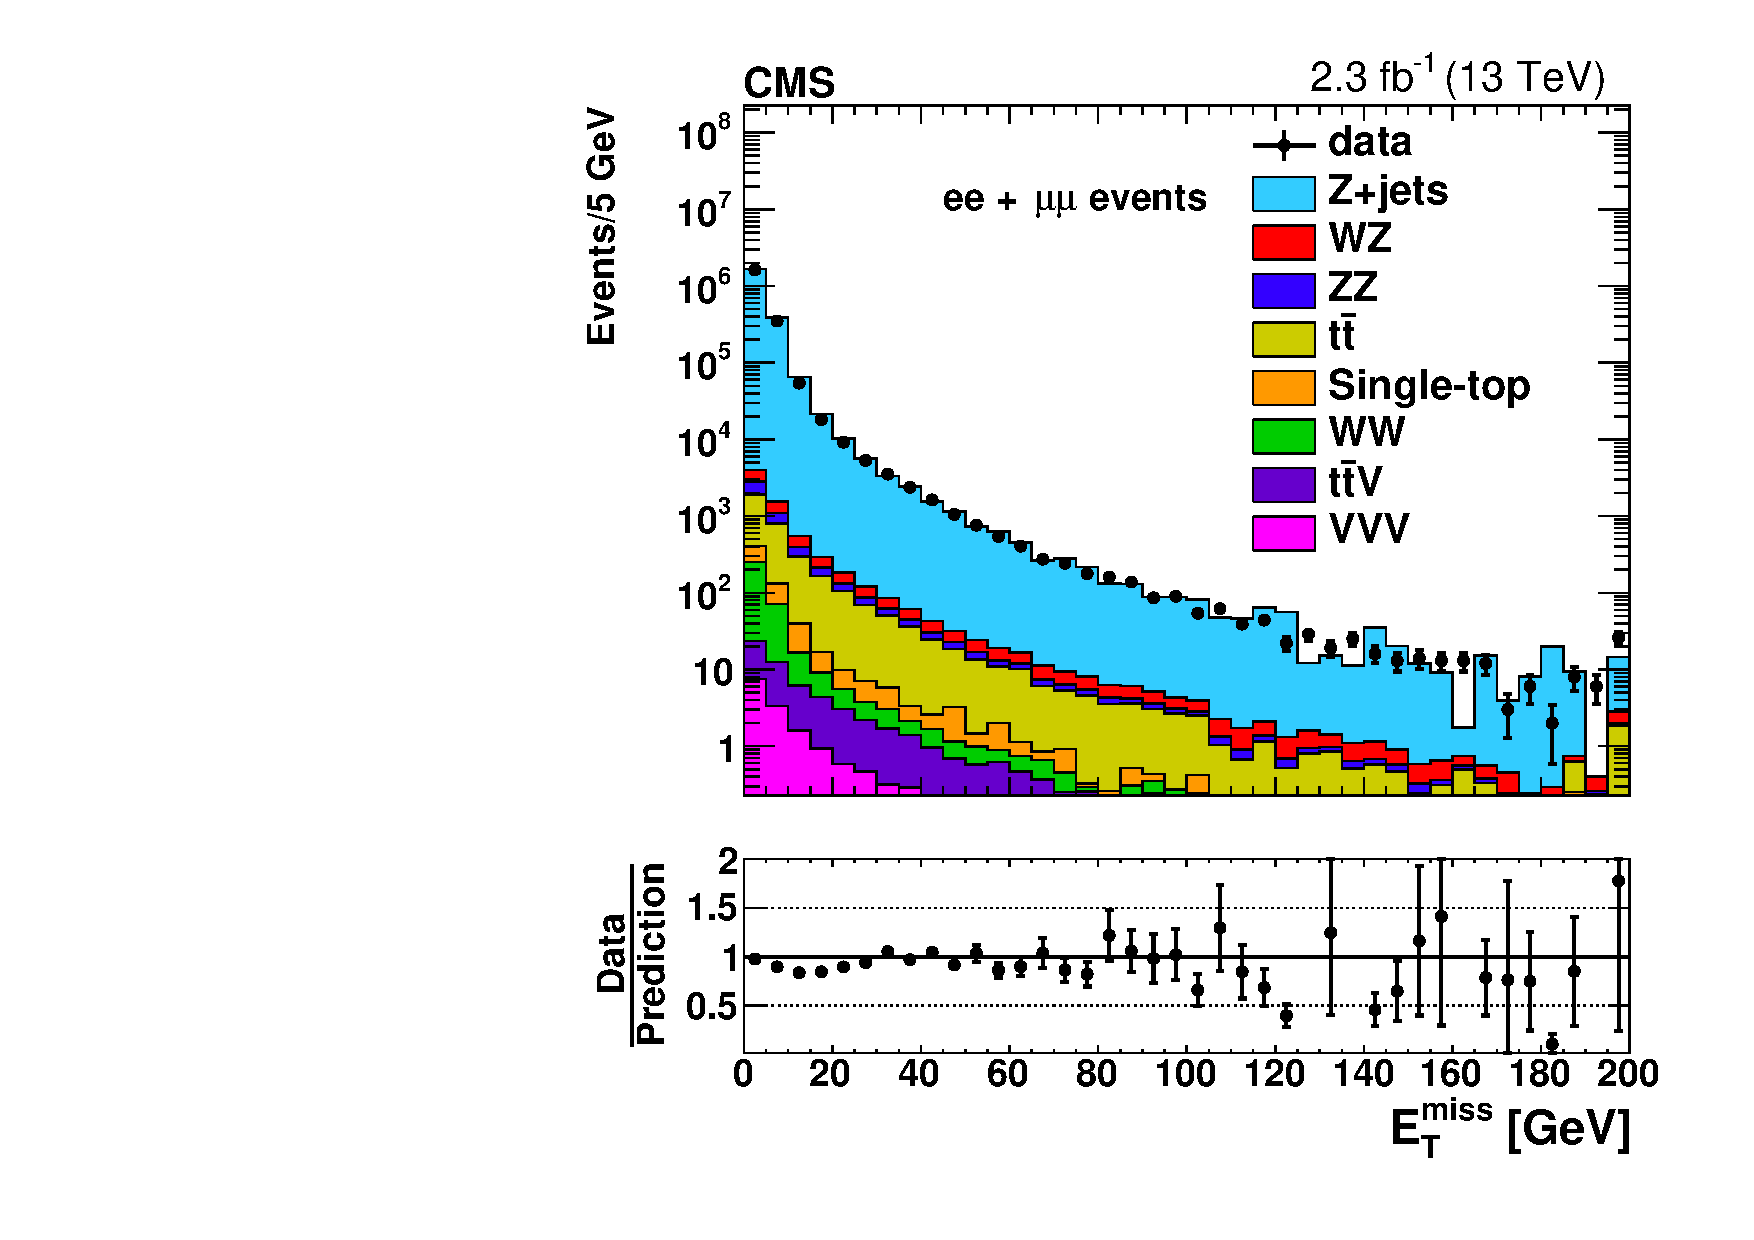
\includegraphics[width=0.4\textwidth]{MET/figs/h_met_phpfcands_1624_pt_ll_signalregion_inclusive_passtrig.pdf} &
      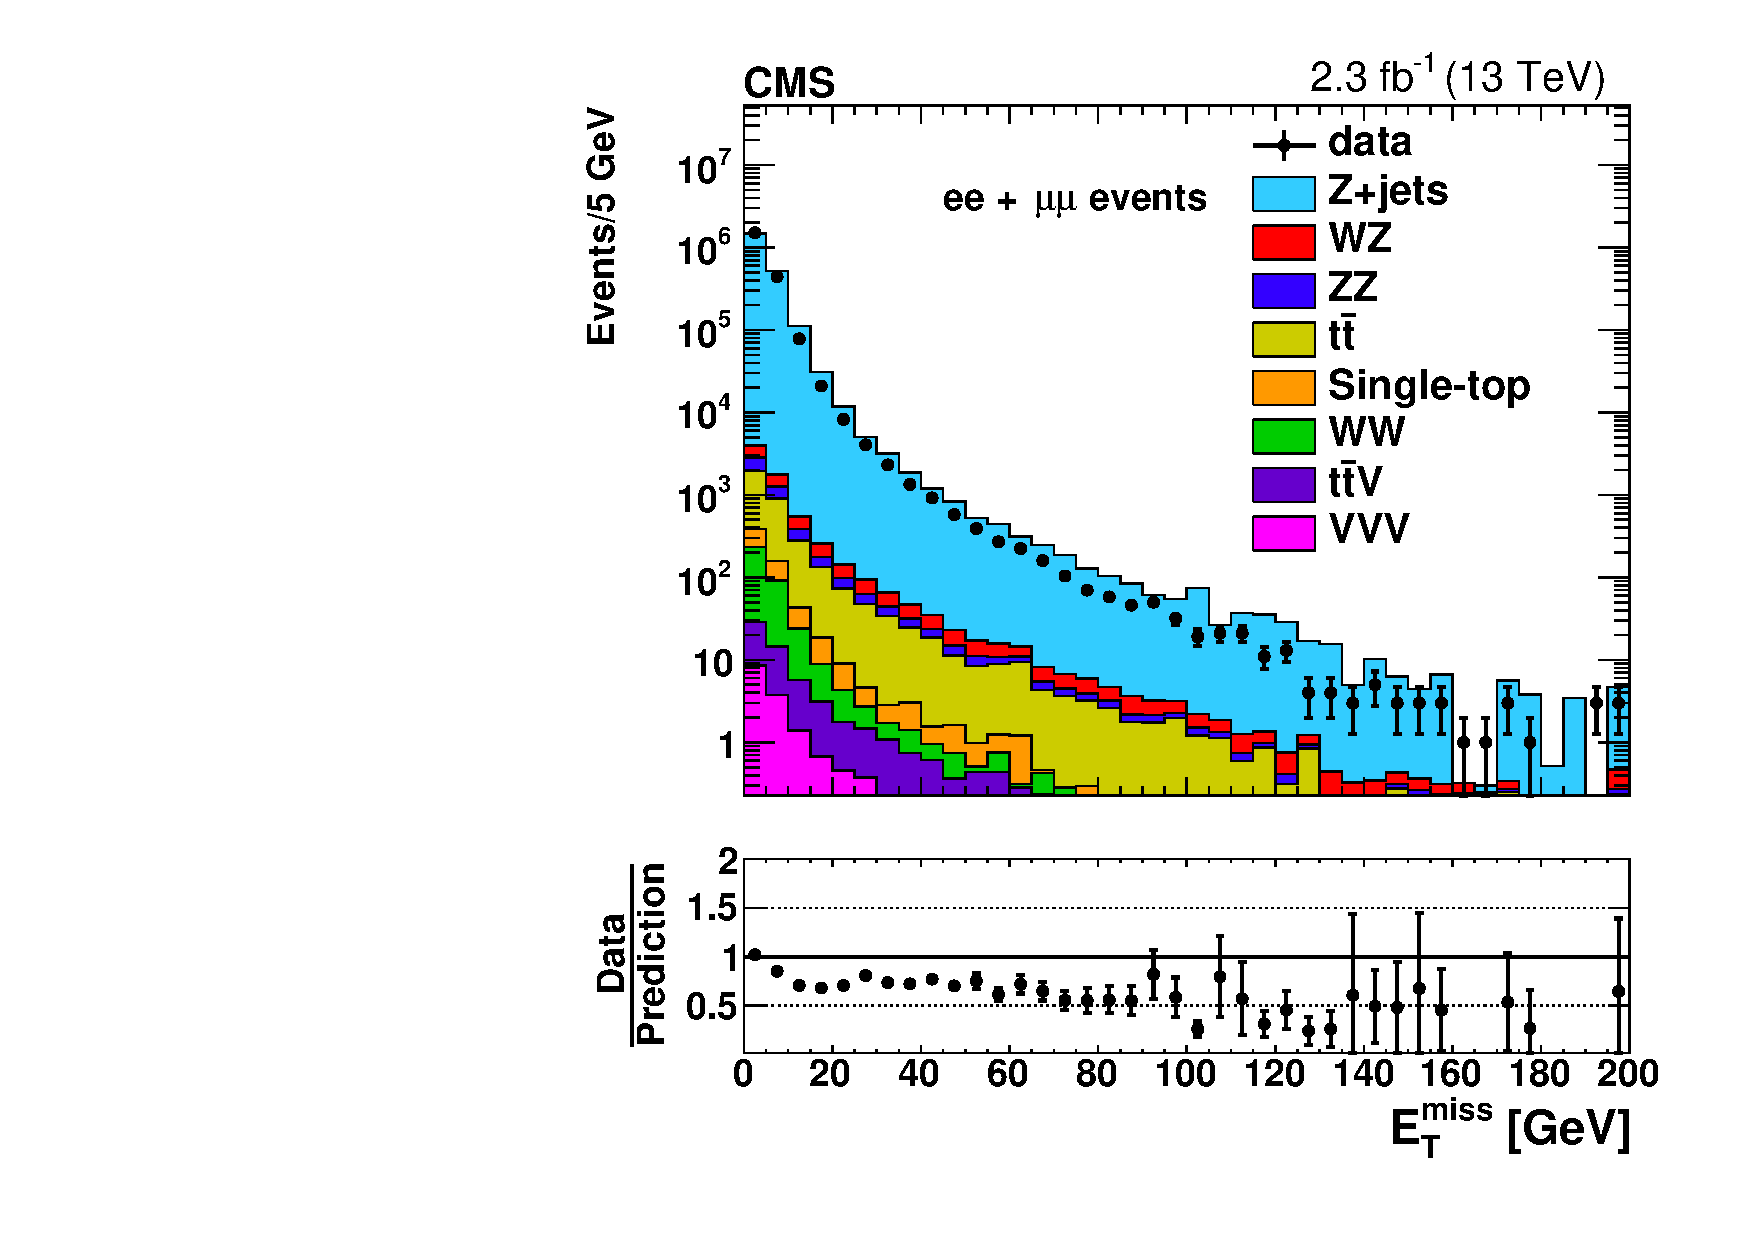
\includegraphics[width=0.4\textwidth]{MET/figs/h_met_phpfcands_2430_pt_ll_signalregion_inclusive_passtrig.pdf} \\
    \end{tabular}
    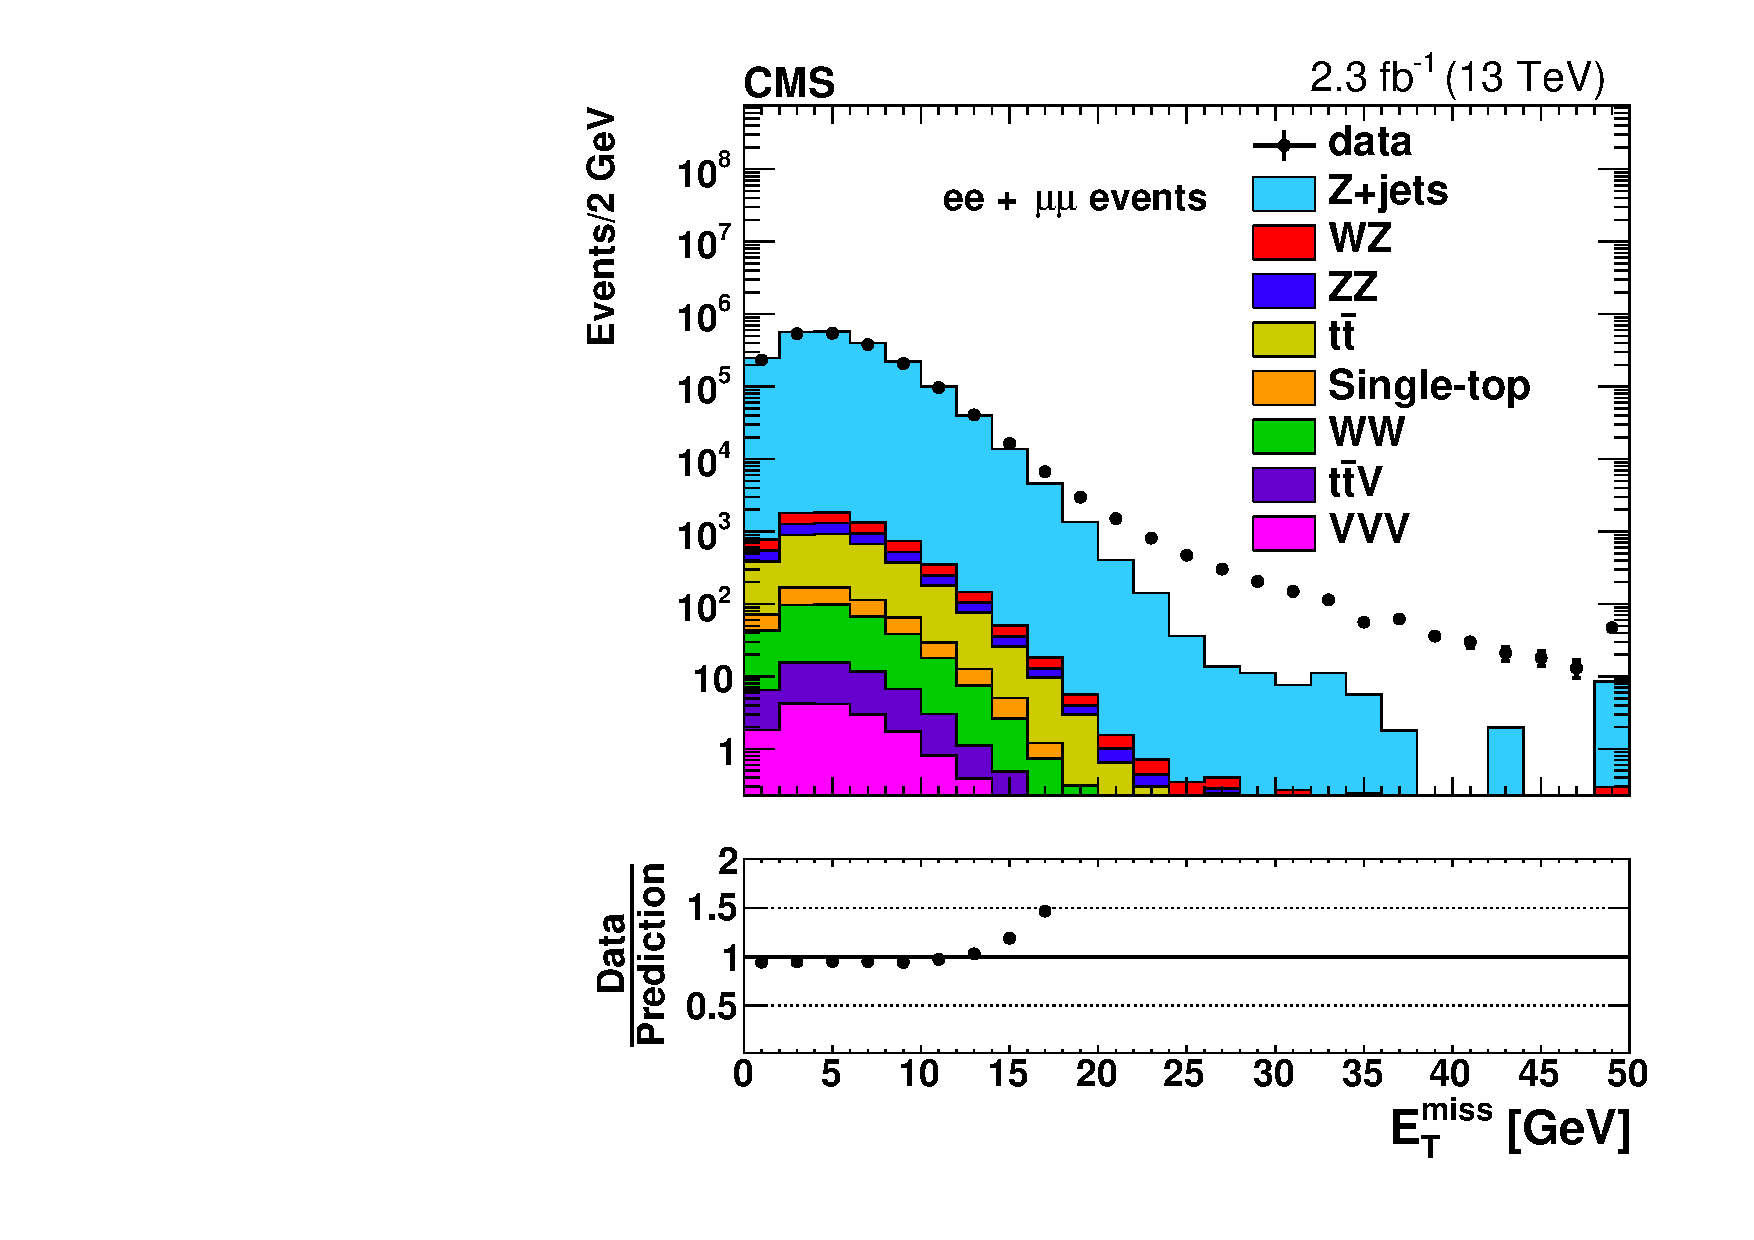
\includegraphics[width=0.4\textwidth]{MET/figs/h_met_phpfcands_30in_pt_ll_signalregion_inclusive_passtrig.pdf} 
    \caption{The \MET\ distribution is shown for neutral electromagnetic PF candidates only.
      The top row shows the barrel region on the left and transition region between the barrel and endcap on the right,
      the second row shows the endcap region including the tracker on the left and endcap region excluding the tracker on the right
      and the bottom row shows the HF region only.
      \label{fig:phpfcands}
    }
  \end{center}
\end{figure}

\begin{figure}[!htb]
  \begin{center}
    \begin{tabular}{cc}
      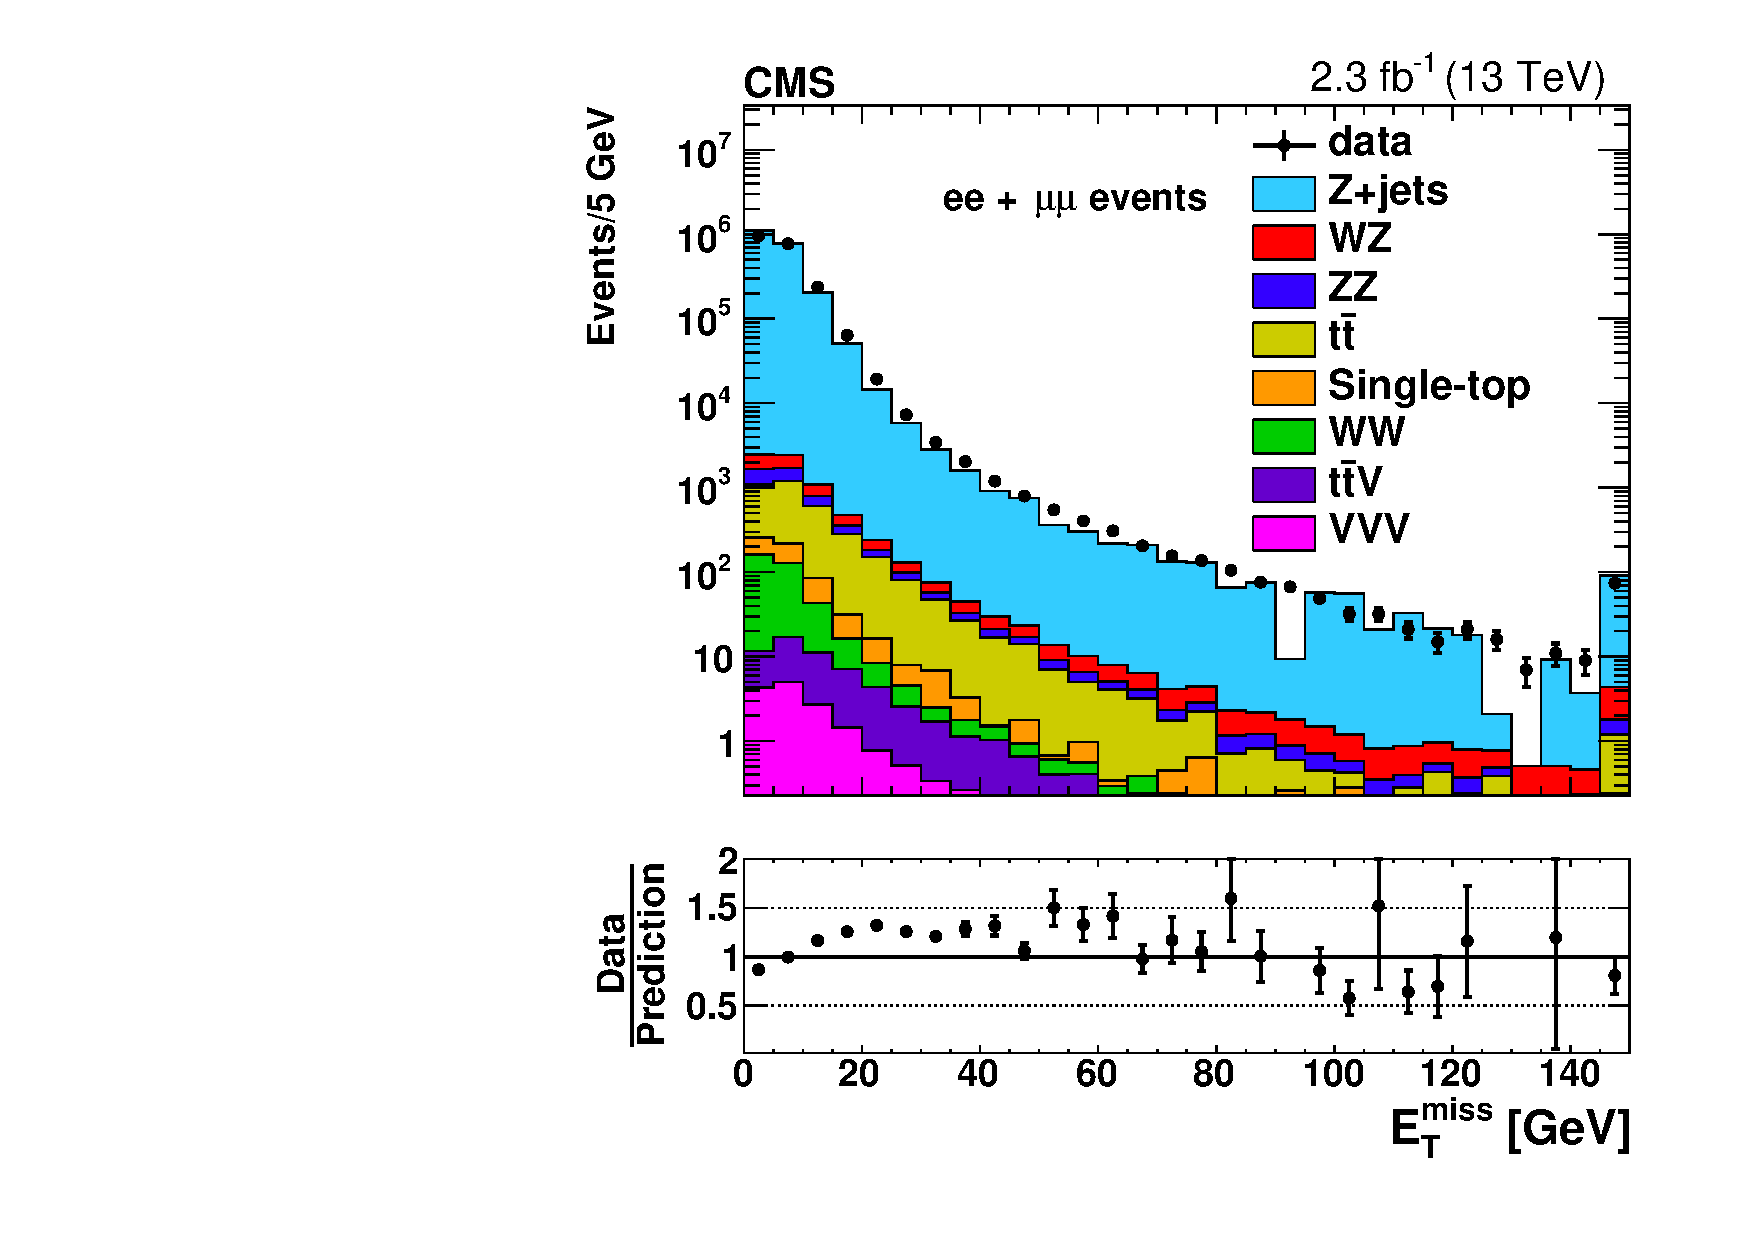
\includegraphics[width=0.4\textwidth]{MET/figs/h_met_nupfcands_0013_pt_ll_signalregion_inclusive_passtrig.pdf} &
      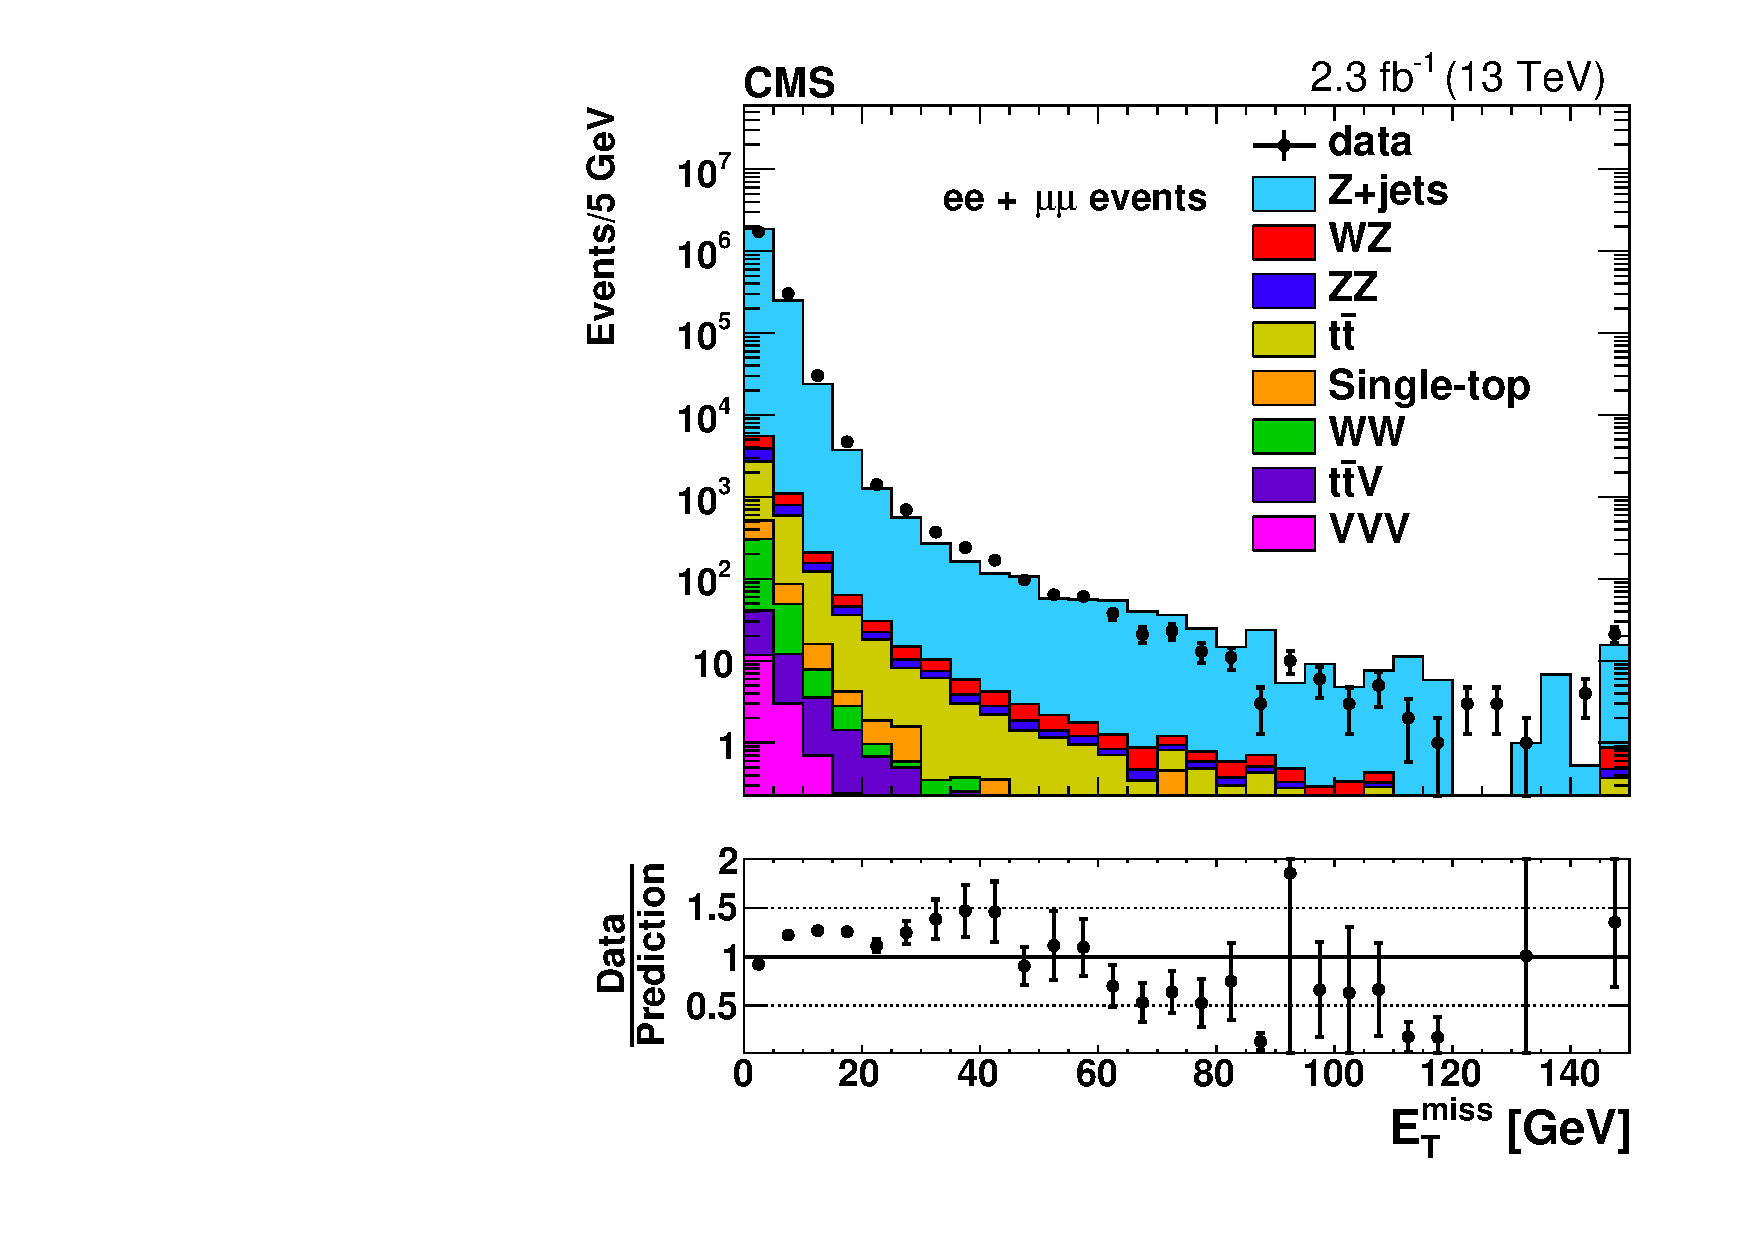
\includegraphics[width=0.4\textwidth]{MET/figs/h_met_nupfcands_1316_pt_ll_signalregion_inclusive_passtrig.pdf} \\
      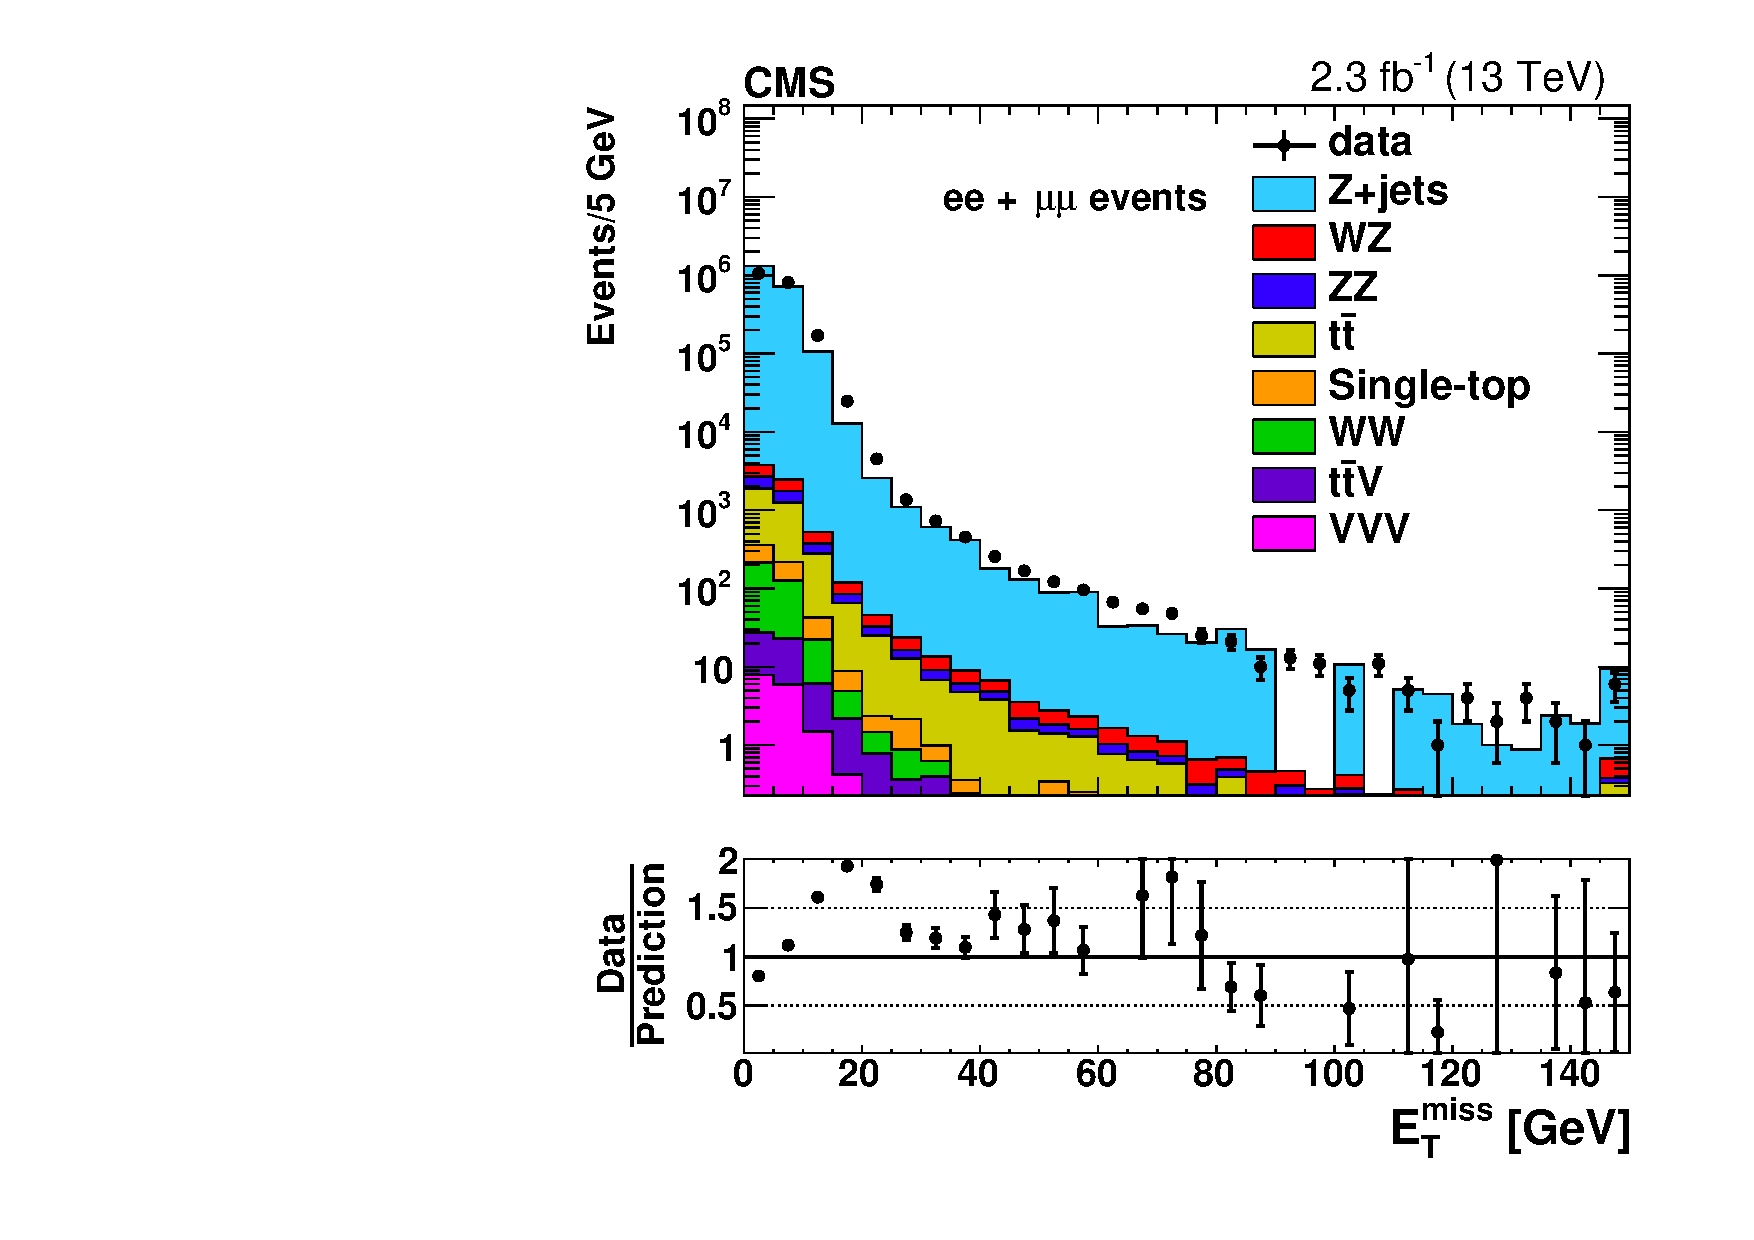
\includegraphics[width=0.4\textwidth]{MET/figs/h_met_nupfcands_1624_pt_ll_signalregion_inclusive_passtrig.pdf} &
      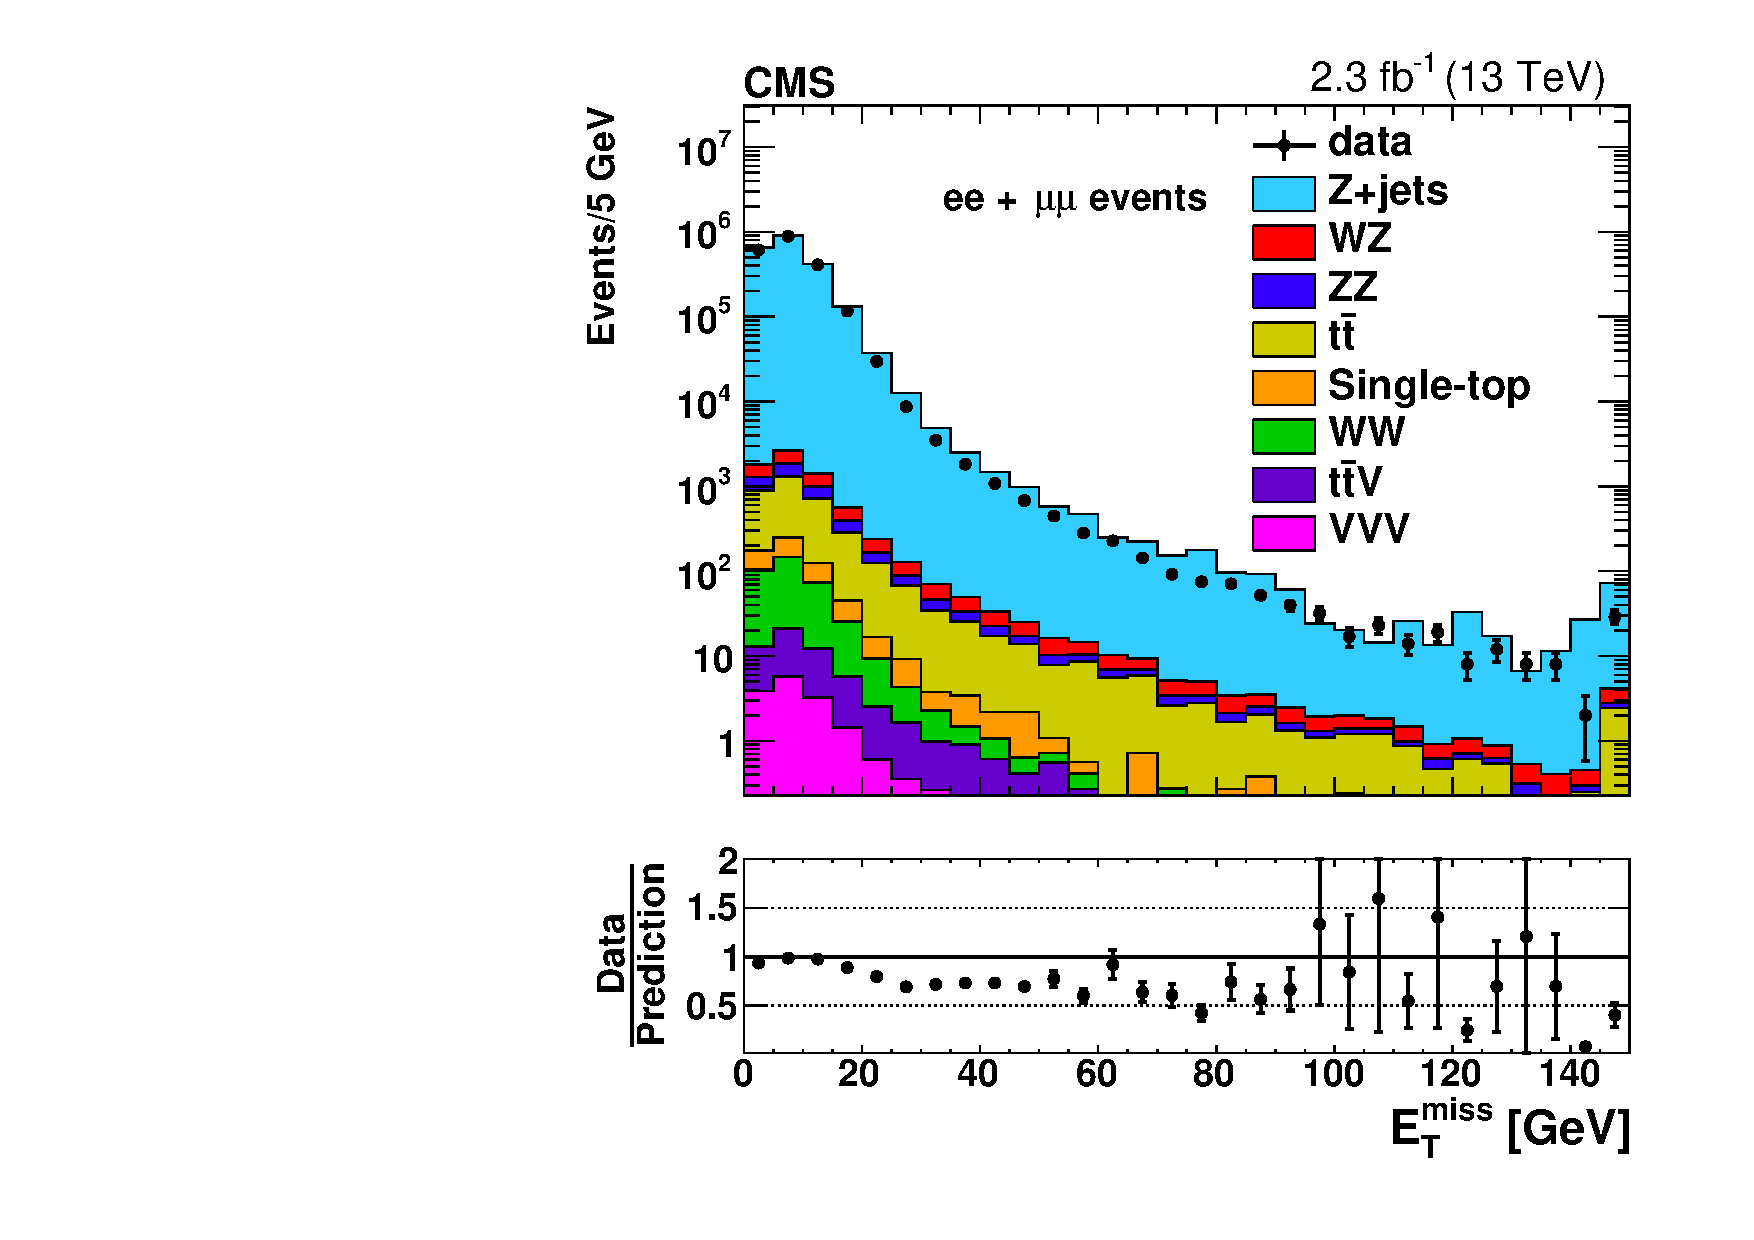
\includegraphics[width=0.4\textwidth]{MET/figs/h_met_nupfcands_2430_pt_ll_signalregion_inclusive_passtrig.pdf} \\
    \end{tabular}
    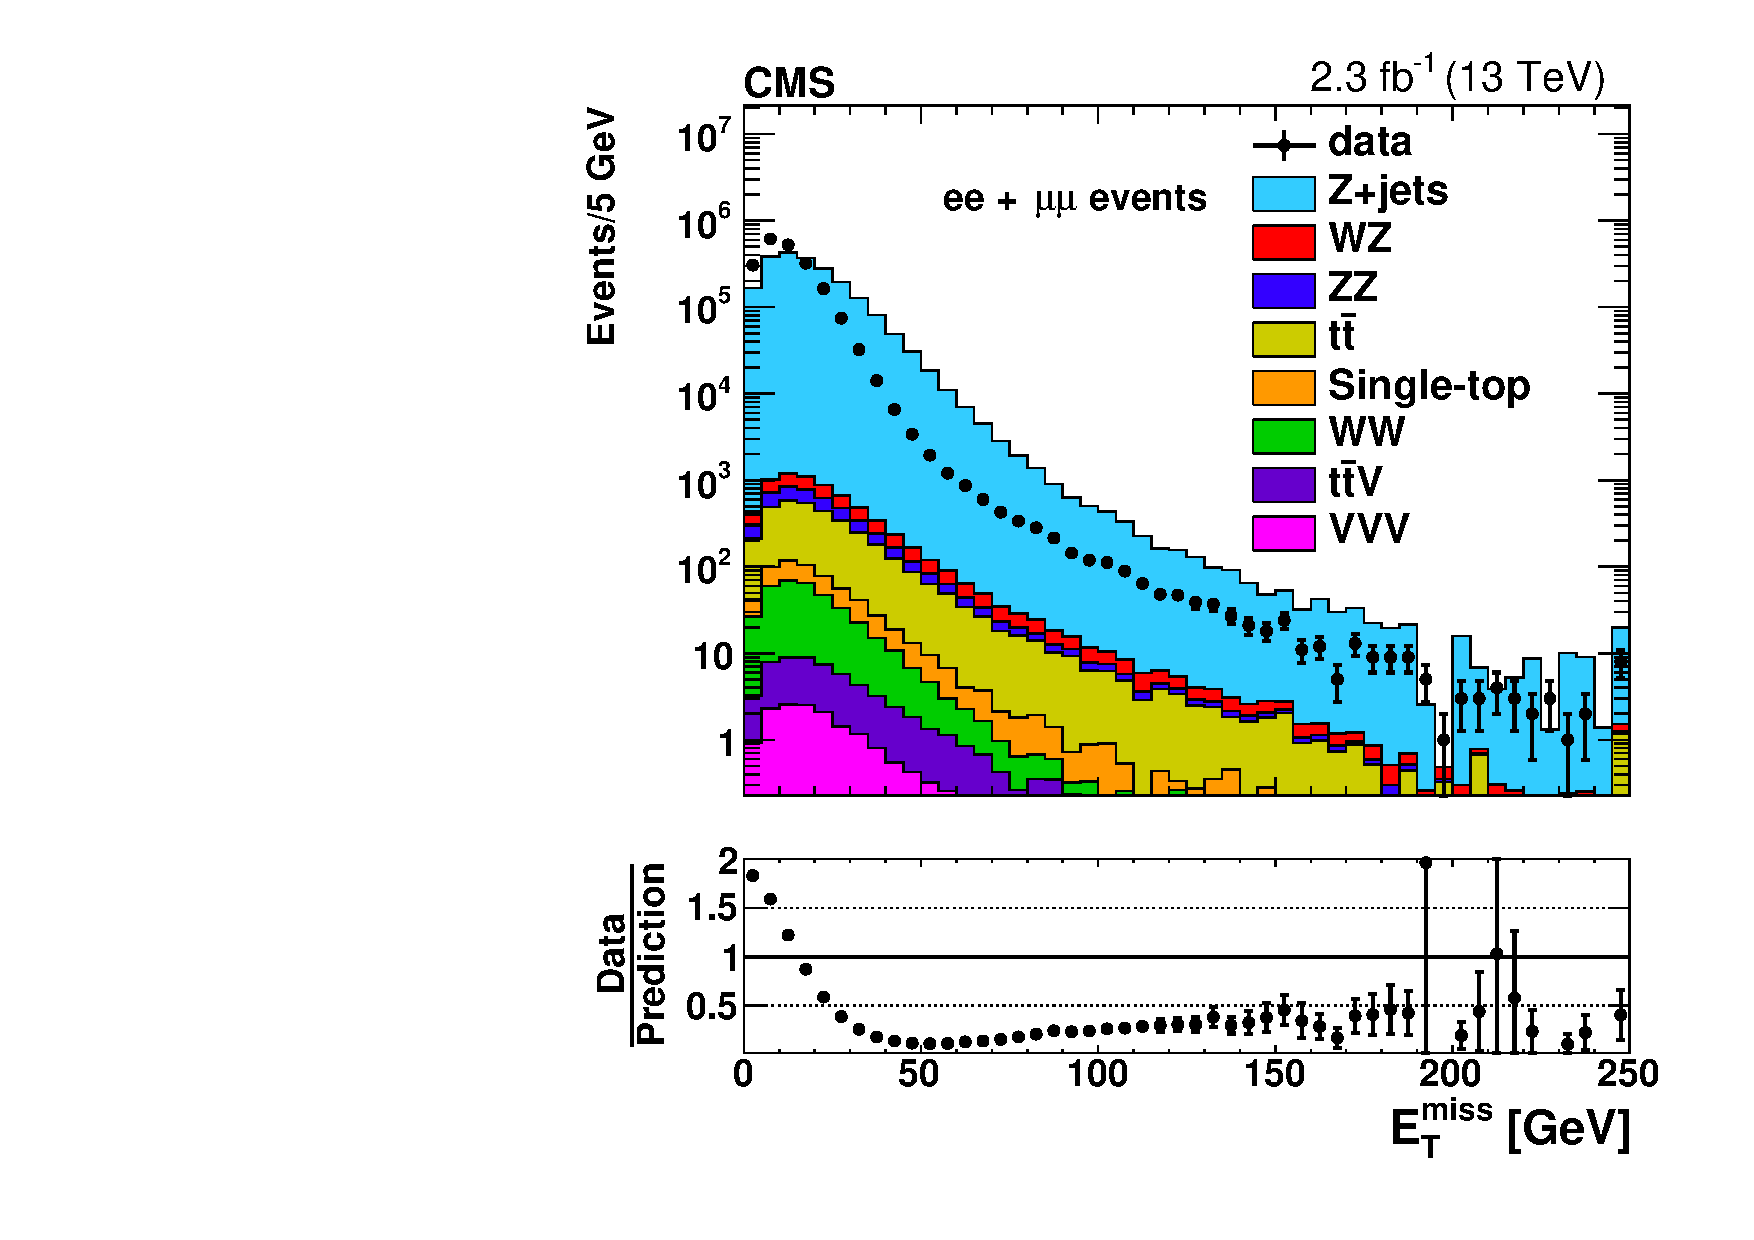
\includegraphics[width=0.4\textwidth]{MET/figs/h_met_nupfcands_30in_pt_ll_signalregion_inclusive_passtrig.pdf} 
    \caption{
      \label{fig:nupfcands}
      The \MET\ distribution is shown for neutral hadronic PF candidates only.
      The top row shows the barrel region on the left and transition region between the barrel and endcap on the right,
      the second row shows the endcap region including the tracker on the left and endcap region excluding the tracker on the right
      and the bottom row shows the HF region only.
    }
  \end{center}
\end{figure}

\clearpage

Finally, the \MET\ distribution is shown after applying the Type-1 corrections as seen in figure~\ref{fig:T1MET_datavsmc}.
Two regions are considered in order to study events with real \MET\ (\MET\ $> 100$ GeV),
and events with fake \MET\ (\MET\ $< 100$ GeV). 
Good agreement is seen in the real \MET\ region,
and reasonable agreement is seen in the fake \MET\ region.

\begin{figure}[!ht]
\begin{center}
\begin{tabular}{cc}
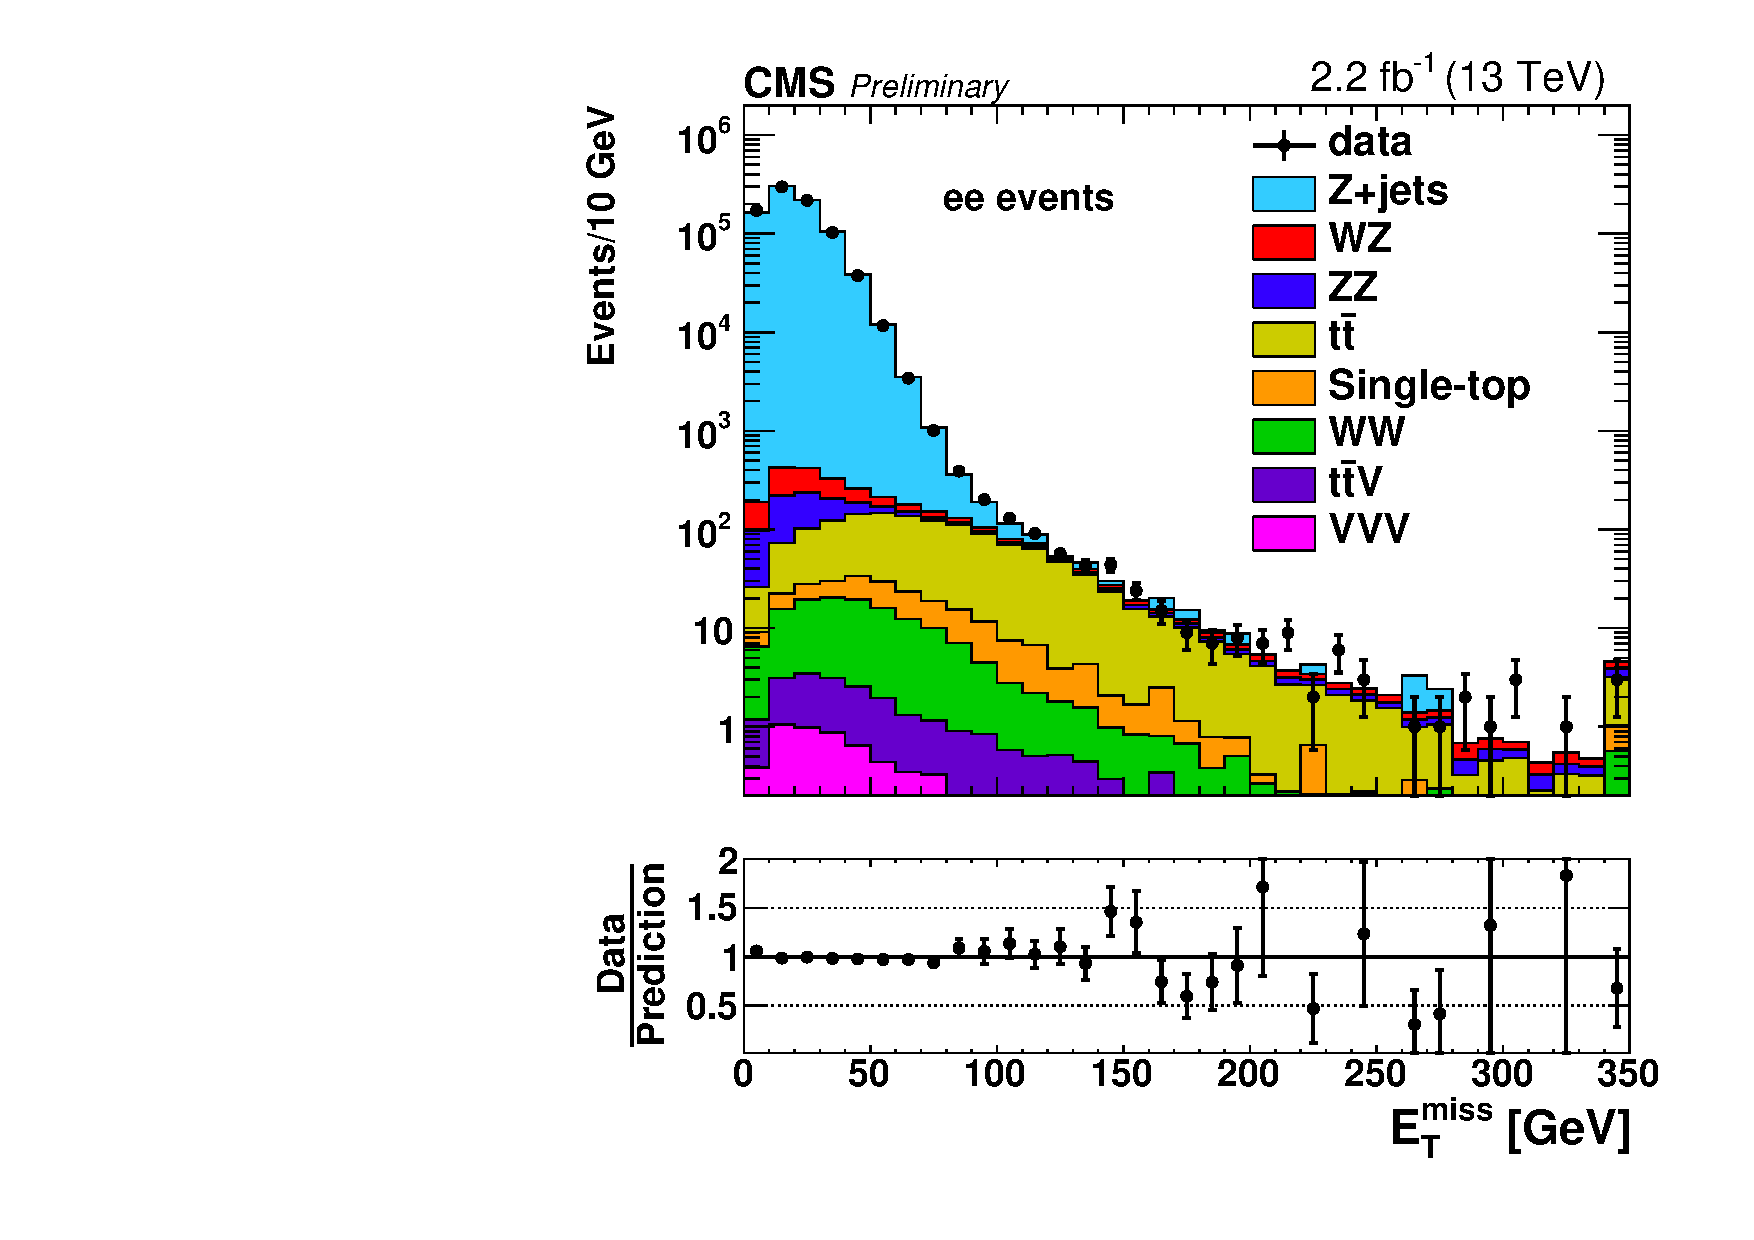
\includegraphics[width=0.4\textwidth]{MET/figs/h_met_T1CHS_pt_ee_inclusive_passtrig.pdf} &
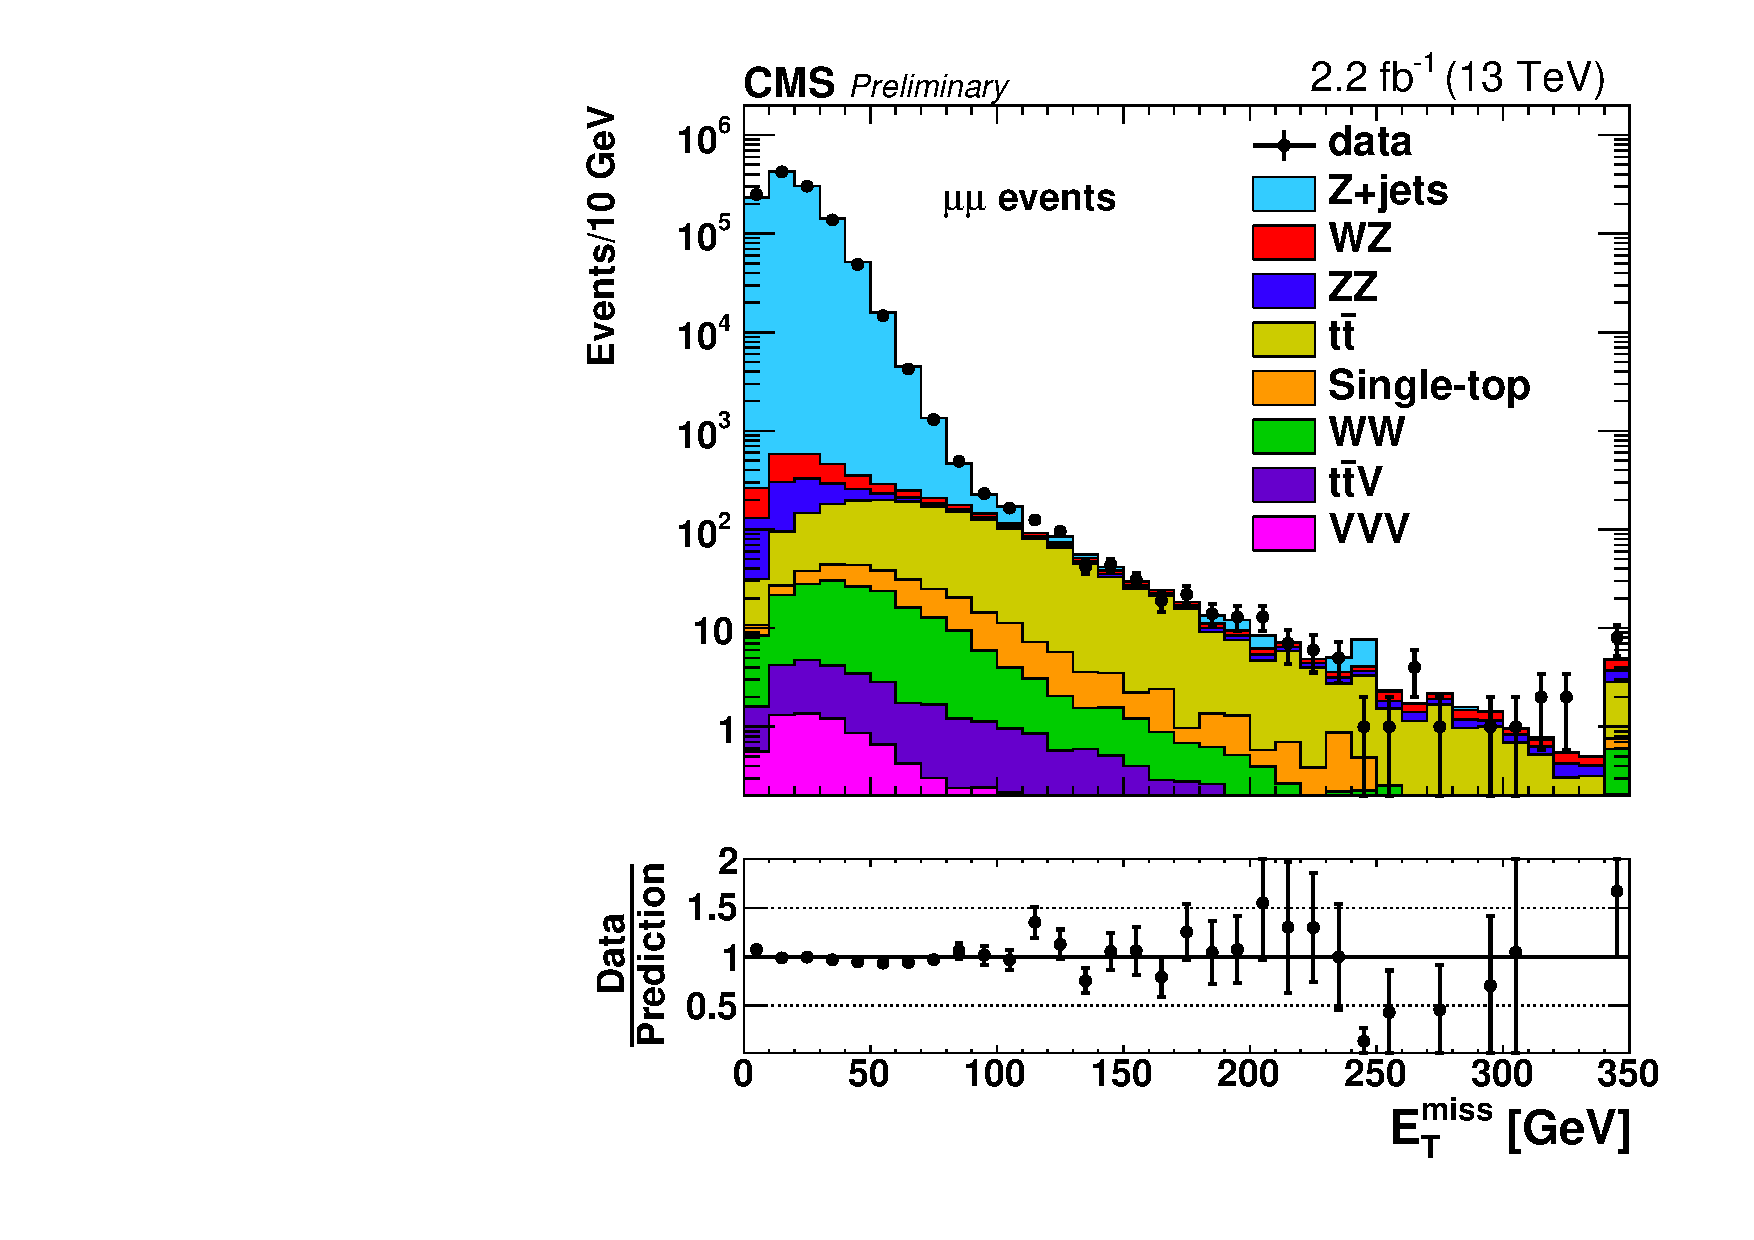
\includegraphics[width=0.4\textwidth]{MET/figs/h_met_T1CHS_pt_mm_inclusive_passtrig.pdf} \\
\end{tabular}
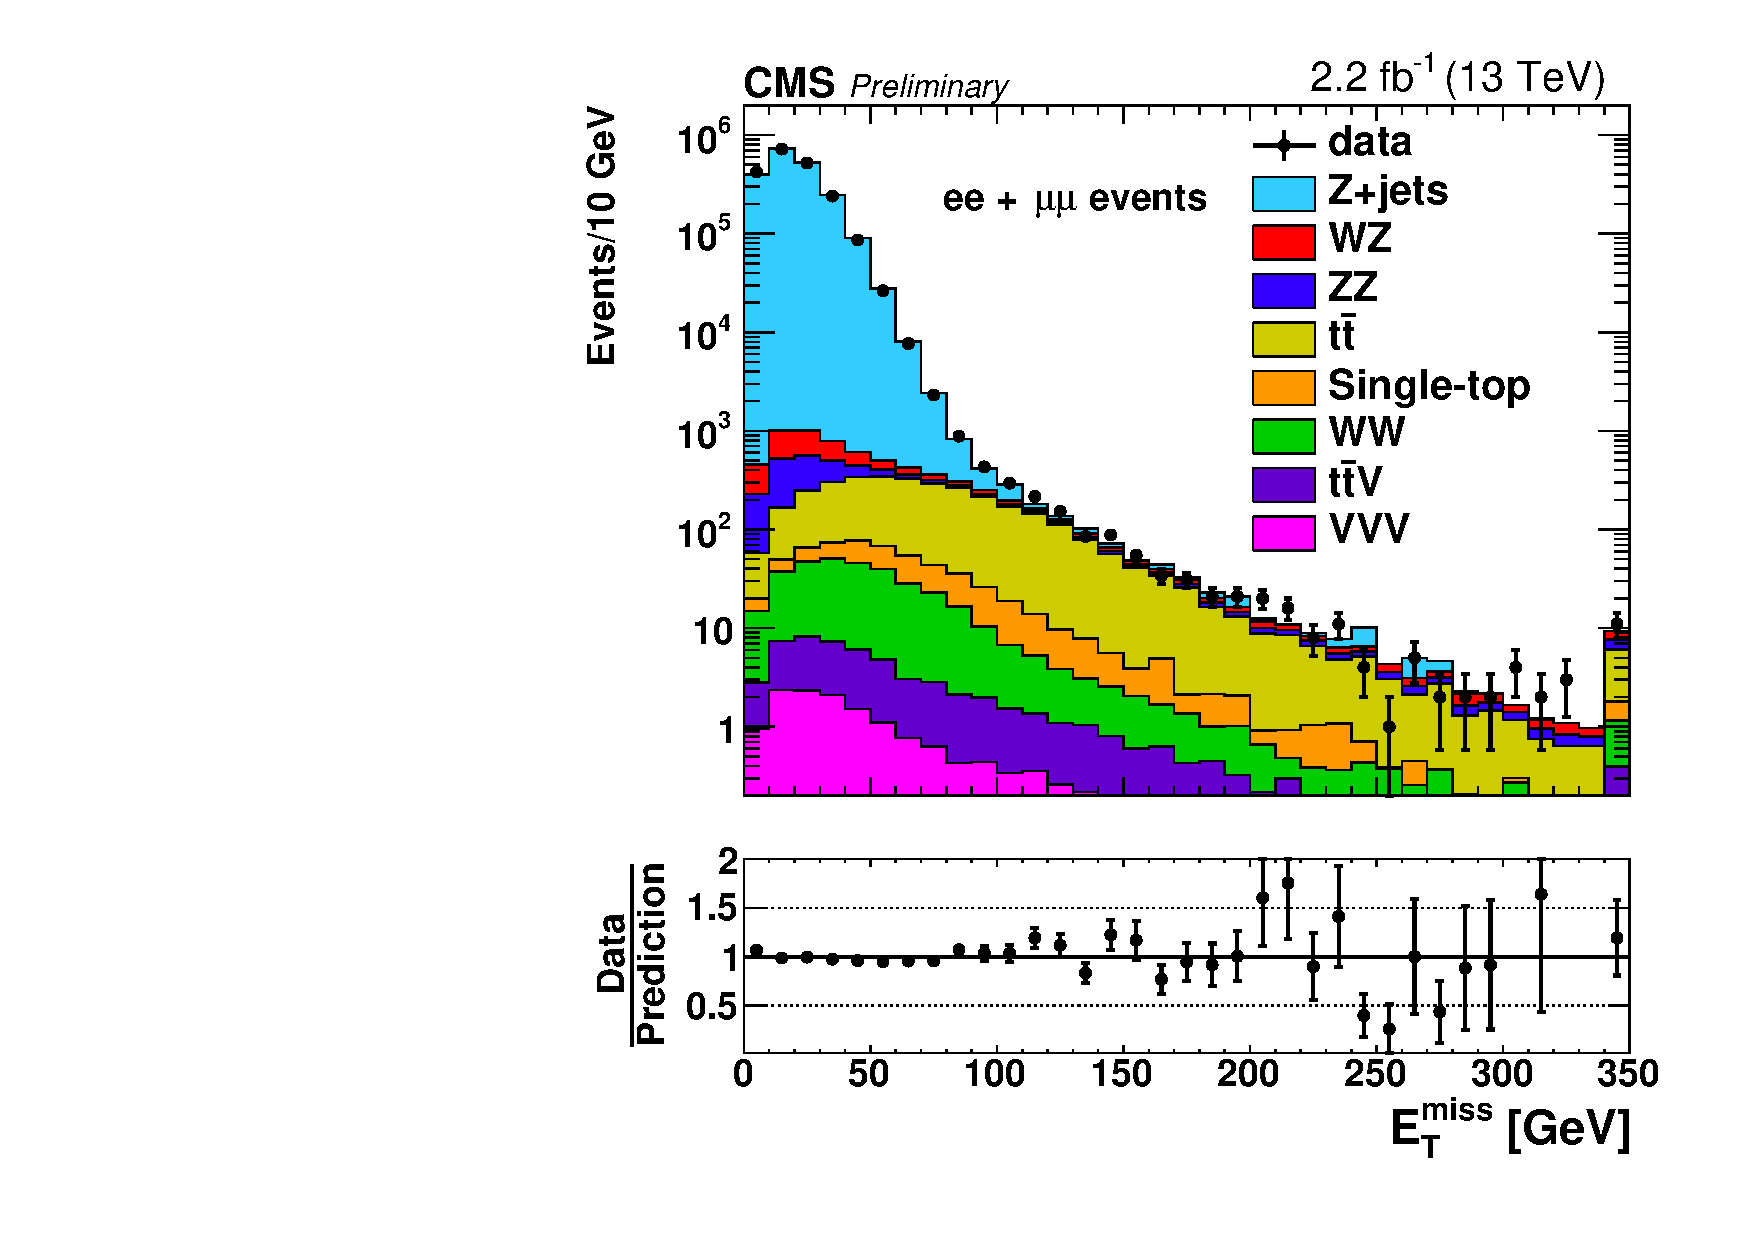
\includegraphics[width=0.6\textwidth]{MET/figs/h_met_T1CHS_pt_ll_inclusive_passtrig.pdf}
\caption{
  The \MET\ distribution is shown with data vs. MC for events while only requirement two leptons with $|M_{\ell\ell}-M_{Z}| < 10 GeV$.
  The top row shows ee events on the left and $\mu\mu$ events on the left,
  and the bottom row shows ee$+\mu\mu$ events together.
  The MC is normalized to data.
\label{fig:T1MET_datavsmc}
}
\end{center}
\end{figure}

\subsection{Data-driven \texorpdfstring{\MET}{MET}\ Predictions}
Although good agreement is seen in data and MC after applying Type-1 corrections to \MET, 
it's clear that there are still problems with the simulation based on the studies in section~\ref{subs:MET_datavsmc}.
Additionally, a new discovery in physics is important enough that it is imperatave that the background predictions can be trusted.
Therefore, it's important to make sure there is a reliable prediction for backgrounds coming from standard model processes in regions with large values of \MET.
Techniques were developed to predict the largest backgrounds using control regions in data,
and these techniques are described in detail in chapter~\ref{ch:bkgd}.

This is to acknowledge all the other members of the CMS experiment who made it possible to produce
the figures and tables appearing in this chapter.

% --------------------------------------------------------------------------- %
% --------------------------------------------------------------------------- %
\chapter{Analysis Selections}
\label{ch:evtsel}
% --------------------------------------------------------------------------- %
% --------------------------------------------------------------------------- %

\section{Triggers and Datasets}
The signal triggers used in this analysis were designed to be maximally efficient for events where a Z boson decays to two leptons.
In order to pass the trigger, at least two leptons with a loose ID and isolation requirement are needed.
Then lepton \pt\ thresholds of the triggers are low enough such that the triggers are fully efficient after making an offline \pt\ cut at 20 \gev\ for both the leading and sub-leading lepton in the event.
In addition to the signal triggers, two other sets of triggers are used in order to collect data in control regions used for data-driven background predictions in the signal region,
and a last set of triggers is used to collect data used to measure the efficiency of the dilepton triggers.
The efficiencies of the ee, e$\mu$ and $\mu\mu$ triggers with respect to the offline selection with two leptons with \pt\ $>$ 20 GeV have been measured as 0.95, 0.94 and 0.93 respectively.
The way this measurement was made is described in section~\ref{sec:bkg_fs}.
All triggers used to collect data for this analysis are listed in table~\ref{table:triggers}.

\begin{itemize}
\item Datasets
  \begin{itemize}
  \item \verb=DoubleEG=
  \item \verb=DoubleMuon=
  \item \verb=MuonEG=
  \item \verb=SinglePhoton=
  \end{itemize}
\item Datasets
  \begin{itemize}
  \item \verb=Run2015C-05Oct2015-v1=
  \item \verb=Run2015D-05Oct2015-v1=
  \item \verb=Run2015D-PromptReco-v4=
  \end{itemize}
\end{itemize}

\begin{table}[htb]
  \begin{center}
    \caption{
      \label{table:triggers}
      A list of all triggers used in this analysis is shown in the table below.
      The signal triggers all require at least two same flavor leptons,
      The control triggers require either at least one photon,
      or at least two different flavor leptons.
    }
    \begin{tabular}{l}
      \hline
      \hline
      {\bf Signal triggers} \\
      \hline
      \verb=HLT_Mu17_TrkIsoVVL_Mu8_TrkIsoVVL_DZ_v*=             \\
      \verb=HLT_Mu17_TrkIsoVVL_TkMu8_TrkIsoVVL_DZ_v*=           \\
      \verb=HLT_Mu27_TkMu8_v*=                                  \\
      \verb=HLT_Ele17_Ele12_CaloIdL_TrackIdL_IsoVL_DZ_v*=       \\
      \verb=HLT_DoubleEle33_CaloIdL_GsfTrkIdVL_MW_v*=           \\
      \hline
      {\bf e$\mu$ triggers} \\
      \hline
      \verb=HLT_Mu17_TrkIsoVVL_Ele12_CaloIdL_TrackIdL_IsoVL_v*= \\
      \verb=HLT_Mu8_TrkIsoVVL_Ele17_CaloIdL_TrackIdL_IsoVL_v*=  \\
      \verb=HLT_Mu30_Ele30_CaloIdL_GsfTrkIdVL_v*=               \\
      \hline
      {\bf single-$\gamma$ triggers} \\
      \hline
      \verb=HLT_Photon22_R9Id90_HE10_IsoM_v*=  \\ 
      \verb=HLT_Photon30_R9Id90_HE10_IsoM_v*=  \\
      \verb=HLT_Photon36_R9Id90_HE10_IsoM_v*=  \\
      \verb=HLT_Photon50_R9Id90_HE10_IsoM_v*=  \\
      \verb=HLT_Photon75_R9Id90_HE10_IsoM_v*=  \\
      \verb=HLT_Photon90_R9Id90_HE10_IsoM_v*=  \\
      \verb=HLT_Photon120_R9Id90_HE10_IsoM_v*= \\
      \verb=HLT_Photon165_R9Id90_HE10_IsoM_v*= \\
      \verb=HLT_Photon165_HE10_v*=             \\
      \hline
      {\bf \HT\ triggers} \\
      \hline
      \verb=HLT_PFHT200_v*= \\
      \verb=HLT_PFHT250_v*= \\
      \verb=HLT_PFHT300_v*= \\
      \verb=HLT_PFHT350_v*= \\
      \verb=HLT_PFHT400_v*= \\
      \verb=HLT_PFHT475_v*= \\
      \verb=HLT_PFHT600_v*= \\
      \verb=HLT_PFHT650_v*= \\
      \verb=HLT_PFHT800_v*= \\
      \verb=HLT_PFHT900_v*= \\
      \hline
      \hline

    \end{tabular}
  \end{center}
\end{table}

\clearpage

\section{Simulations from Monte-Carlo}
The CMS detector is simulated using the Geant4 toolbox~\cite{Geant}, and various physics processes are simulated.
This simulation keeps track of energies deposited by each particle,
above a certain threshold, as the incident particle's shower progresses through detector materials.
This is process is very computationally intensive and time consuming,
so an alternative method of simulation using parameterized shapes of particle showers, named FastSim, was developed.
The simulation is composed of the following steps
\begin{itemize}
\item Modeling the Interaction Region
\item Modeling the particles passage through the hierarchy of volumes that compose CMS detector and of the accompanying physics processes
\item Modeling the effects of multiple interactions per beam crossing and/or the effect of events overlay (PileUp simulation)
\item Modeling the detector's electronics response (digitization)
\end{itemize}

The actual simulation of the physics process is done using a variety of different software where the various packages used perform differently at simulating certain physics effects.
In this analysis, \ttbar\ events are simulated using powheg~\cite{powheg} and Drell-Yan processes are simulated using MadGraph~\cite{aMCatNLO}.
The matrix element calculations performed with these generators are then interfaced with pythia 8~\cite{Pythia} for the simulation of parton showering and hadronization.

After selecting events with two leptons, data is compared to MC and good agreement can be seen in the plots shown in section~\ref{ssec:datavsmc}.
Cross sections and k-factors are applied to MC backgrounds to normalize them to the calculated luminosity of the signal triggers used to take data in 2015, which is 2.3 $\mathrm{fb^{-1}}$.
Cross section values are calculated using the FEWZ software package~\cite{Li:2012wna},
and factors are derived by comparing data to MC in control regions in order to correct the MC for beyond leading-order effects. %%https://twiki.cern.ch/twiki/bin/viewauth/CMS/SummaryTable1G25ns
The events from MC are required to pass the same triggers as in data where the triggers are simulated in the MC,
and the MC is then reweighted to accurately represent the number of pileup events in data.

\begin{sidewaystable}[htb]                                                                                                                                                              
\begin{center}                                                                                                                                                
%% \scriptsize
  \caption{
    \label{tab:mcsamples}
    A list of MC samples used in this analysis are shown in this table.
    The MC samples used for background studies are all made with different generators,
    depending on which physics process that is being modeled.
    The signal MC is produced using the FastSim package.
  }
\begin{tabular}{l|l|l}  
\hline
\hline
Process     & Dataset Name                                                                & Cross Section [pb] \\
\hline
\zjets      & \verb=/DYJetsToLL_M-10to50_TuneCUETP8M1_13TeV-amcatnloFXFX-pythia8/*=       & 18610        \\
            & \verb=/DYJetsToLL_M-50_TuneCUETP8M1_13TeV-amcatnloFXFX-pythia8/*=           & 6104         \\
\hline
\ttbar      & \verb=/TTTo2L2Nu_13TeV-powheg/*=                                            & 87.31483776  \\
\hline
ZZ          & \verb=/ZZTo4L_13TeV_powheg_pythia8*=                                        & 1.256        \\
            & \verb=/ZZTo2L2Q_13TeV_amcatnloFXFX_madspin_pythia8/*=                       & 3.38         \\
            & \verb=/ZZTo2L2Nu_13TeV_powheg_pythia8/*=                                    &              \\
\hline
WZ          & \verb=/WZTo2L2Q_13TeV_amcatnloFXFX_madspin_pythia8/*=                       & 5.52         \\
            & \verb=/WZTo3LNu_TuneCUETP8M1_13TeV-powheg-pythia8/*=                        & 4.42965      \\
\hline
WW          & \verb=/WWTo2L2Nu_13TeV-powheg/*/=                                           & 118.7        \\
\hline
single top  & \verb=/ST_tW_top_5f_inclusiveDecays_13TeV-powheg-pythia8/*=                 & 38.09        \\
            & \verb=/ST_tW_antitop_5f_inclusiveDecays_13TeV-powheg-pythia8/*=             & 38.09        \\
\hline
${\ttbar}$V & \verb=/TTWJetsToLNu_TuneCUETP8M1_13TeV-amcatnloFXFX-madspin-pythia8/*=      & 0.2043       \\
            & \verb=/TTWJetsToQQ_TuneCUETP8M1_13TeV-amcatnloFXFX-madspin-pythia8/*=       & 0.40620      \\
            & \verb=/TTGJets_TuneCUETP8M1_13TeV-amcatnloFXFX-madspin-pythia8/*=           & 3.697        \\
            & \verb=/TTZToQQ_TuneCUETP8M1_13TeV-amcatnlo-pythia8/*=                       & 0.5297       \\
            & \verb=/TTZToLLNuNu_M-10_TuneCUETP8M1_13TeV-amcatnlo-pythia8/*=              & 0.2529       \\
            & \verb=/ttHToNonbb_M125_13TeV_powheg_pythia8/*=                              & 0.5085       \\
\hline
VVV         & \verb=/ZZZ_TuneCUETP8M1_13TeV-amcatnlo-pythia8/*=                           & 0.01398      \\
            & \verb=/WWZ_TuneCUETP8M1_13TeV-amcatnlo-pythia8/*=                           & 0.1651       \\
            & \verb=/WZZ_TuneCUETP8M1_13TeV-amcatnlo-pythia8/*=                           & 0.05565      \\
\hline
            & \verb=*RunIISpring15MiniAODv2-74X_mcRun2_asymptotic_v2-v*/MINIAODSIM=       &              \\
\hline
Signal      & \verb=SMS-T5ZZ_mGluino-*_mLSP-*_TuneCUETP8M1_13TeV-madgraphMLM-pythia8=     & See~\cite{gluinoxsec13tev} \\
\hline
\hline
\end{tabular}
\end{center}
\end{sidewaystable}

\clearpage

\subsection{Data vs. MC Comparison}
\label{ssec:datavsmc}
data is compared to MC simulation for many kinematic variables relevant to the search.

\begin{figure}[!ht]
  \begin{center}
    \begin{tabular}{cc}
      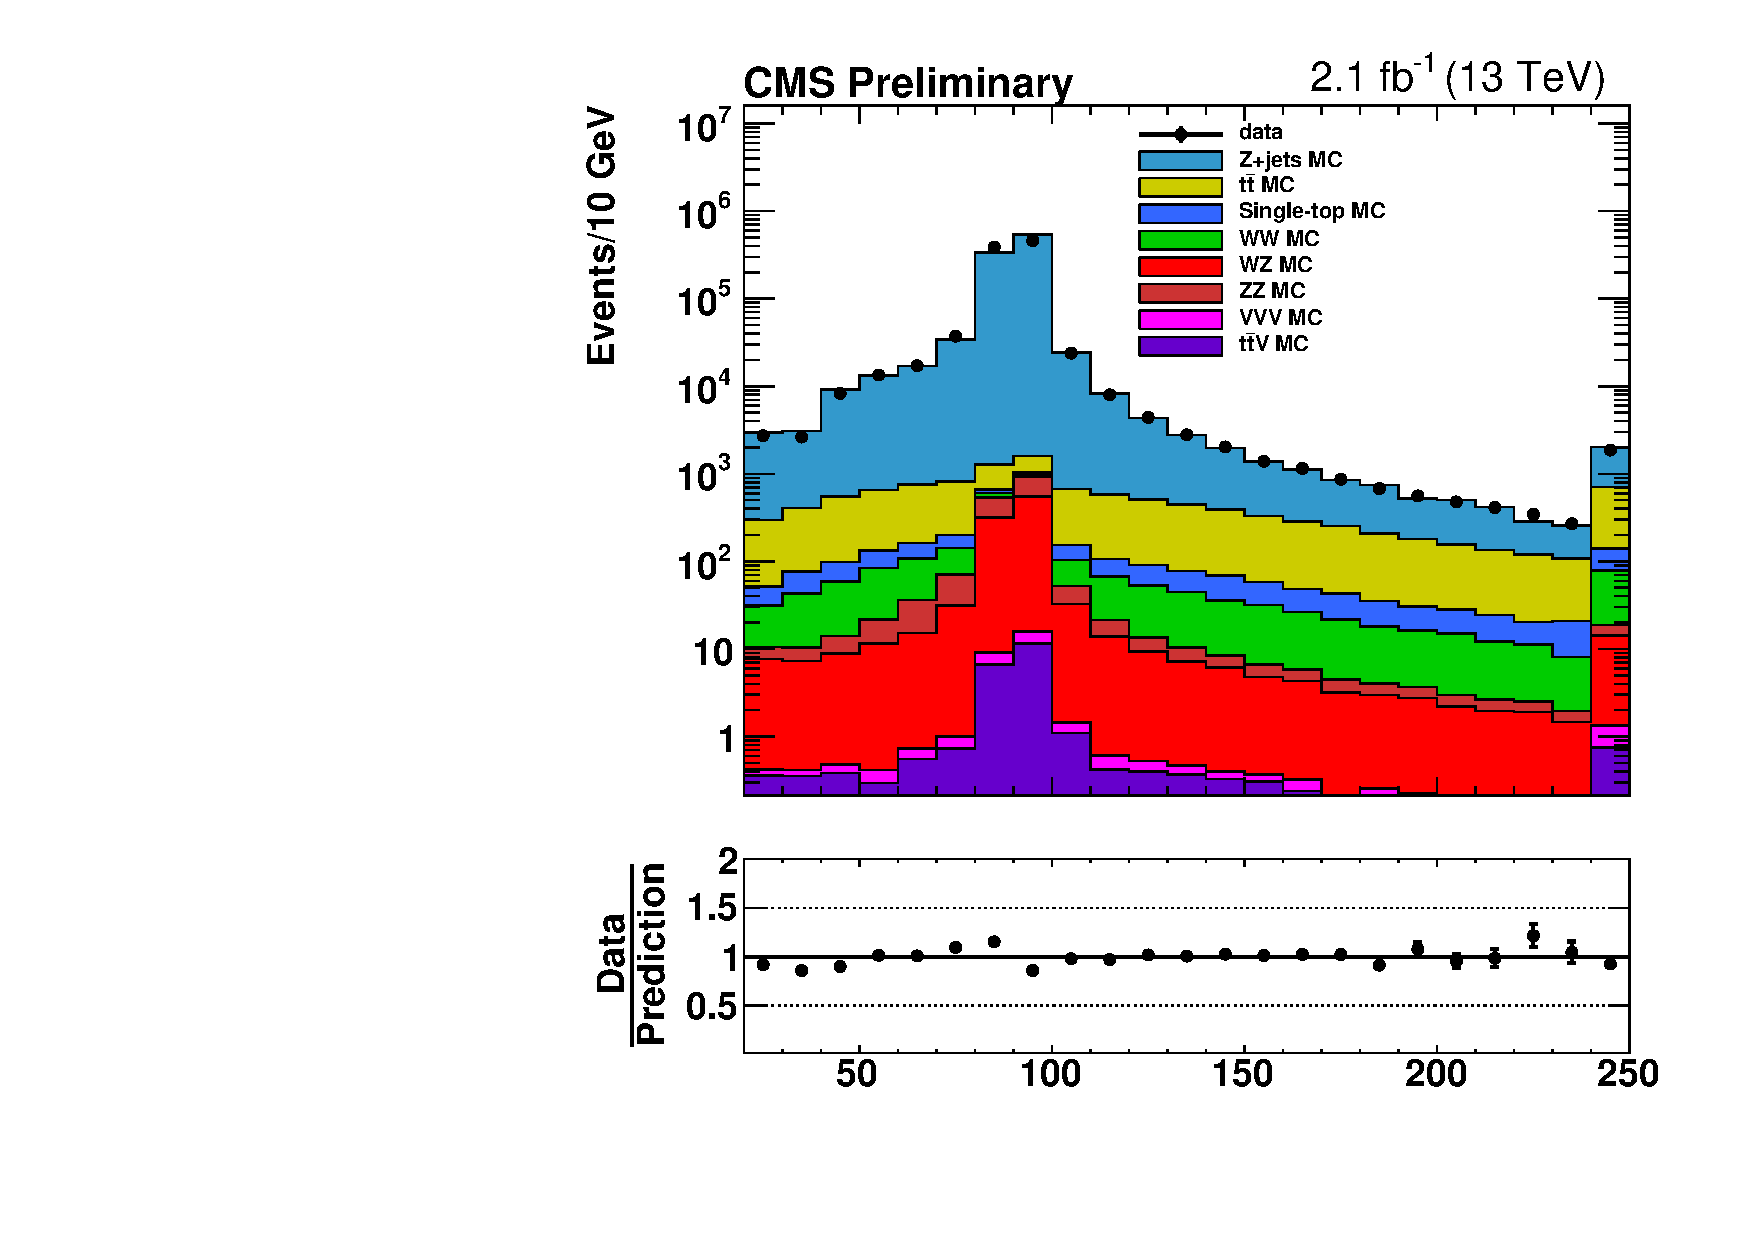
\includegraphics[width=0.4\linewidth]{evtsel/figs/h_mll_ee_signalregion_inclusive_passtrig.pdf} &
      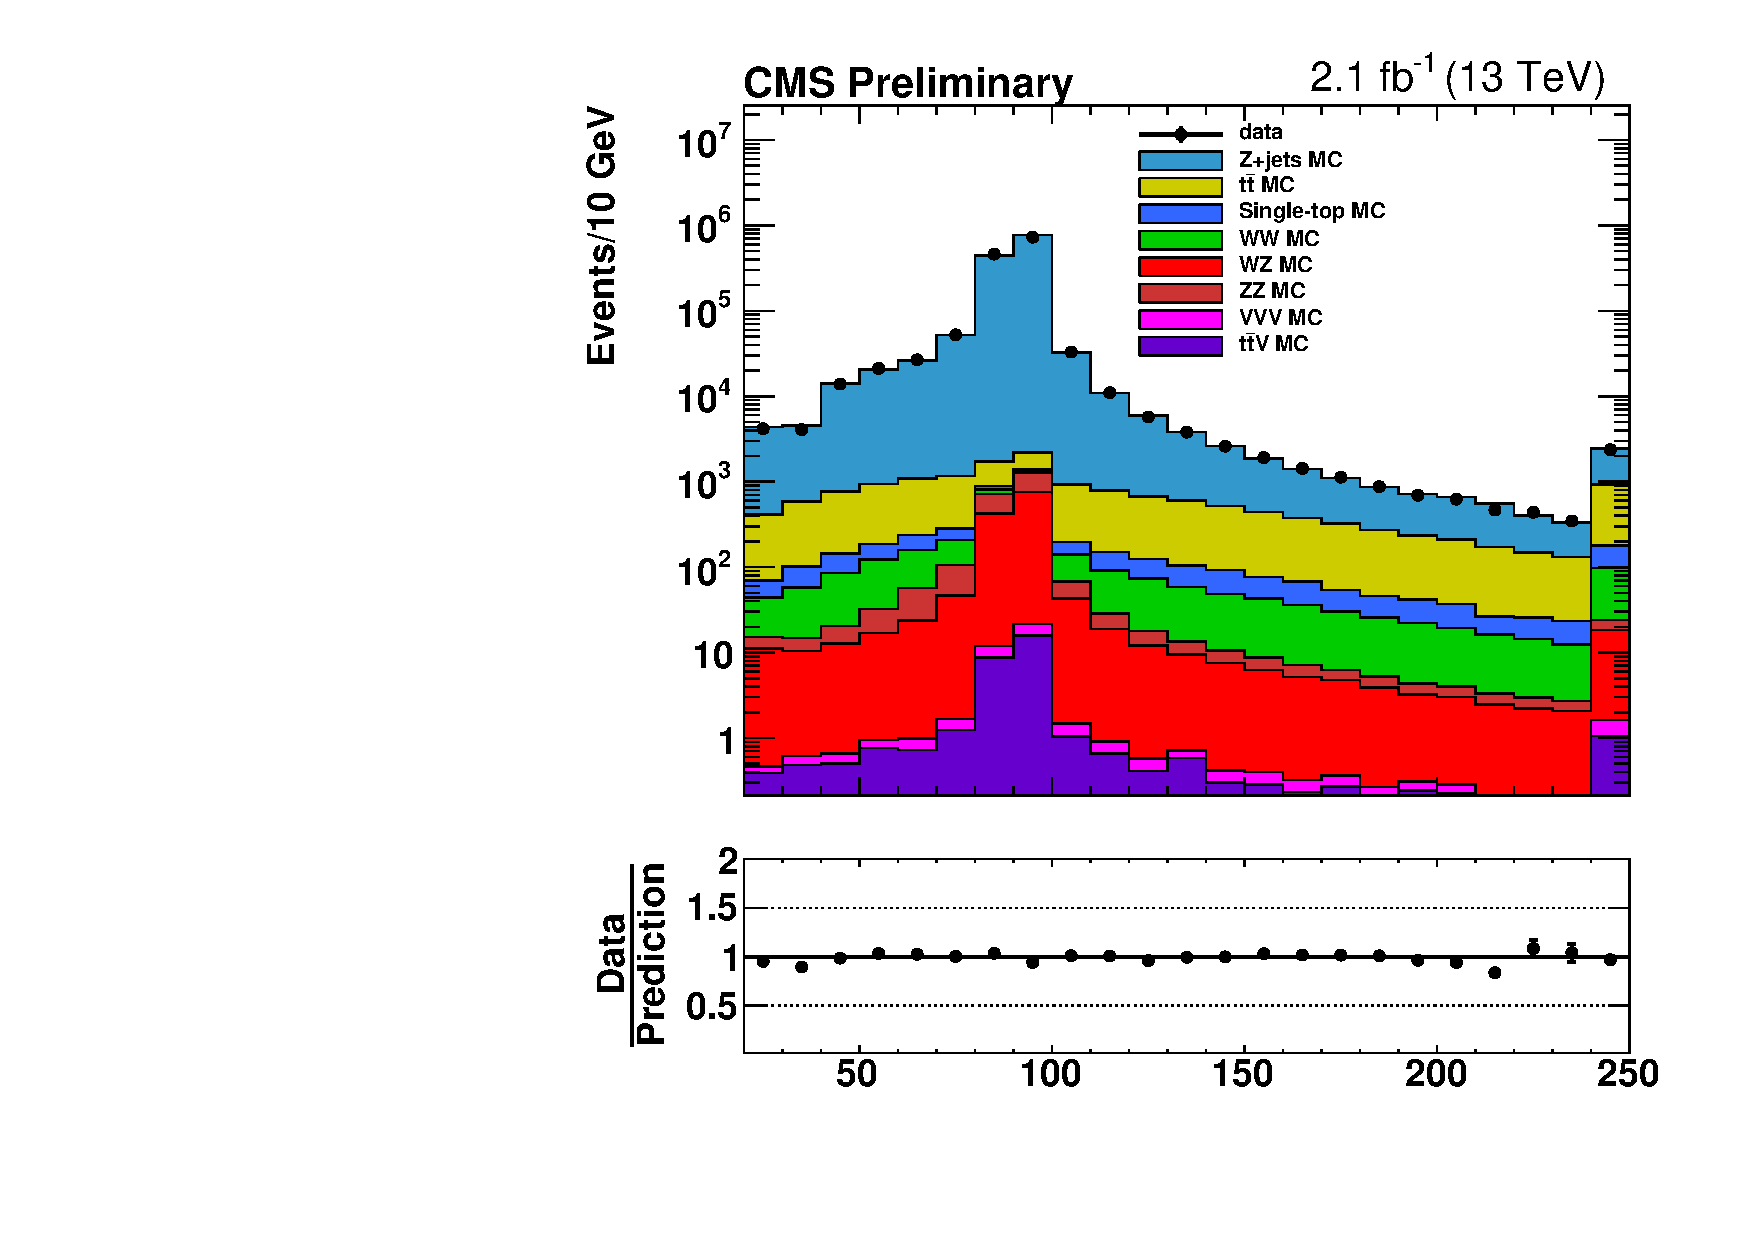
\includegraphics[width=0.4\linewidth]{evtsel/figs/h_mll_mm_signalregion_inclusive_passtrig.pdf} \\
    \end{tabular}
    \caption{
      \label{fig:datavsmc_mll_eemm}
      Data vs. MC comparison showing \mll\ with ee events on the left and $\mu\mu$~events on the right.
      For this analysis, a cut is required that $|M_{\ell\ell}-M_{Z}| < 10 GeV$.
    }
  \end{center}
\end{figure}

\begin{figure}[!ht]
  \begin{center}
    \begin{tabular}{cc}
      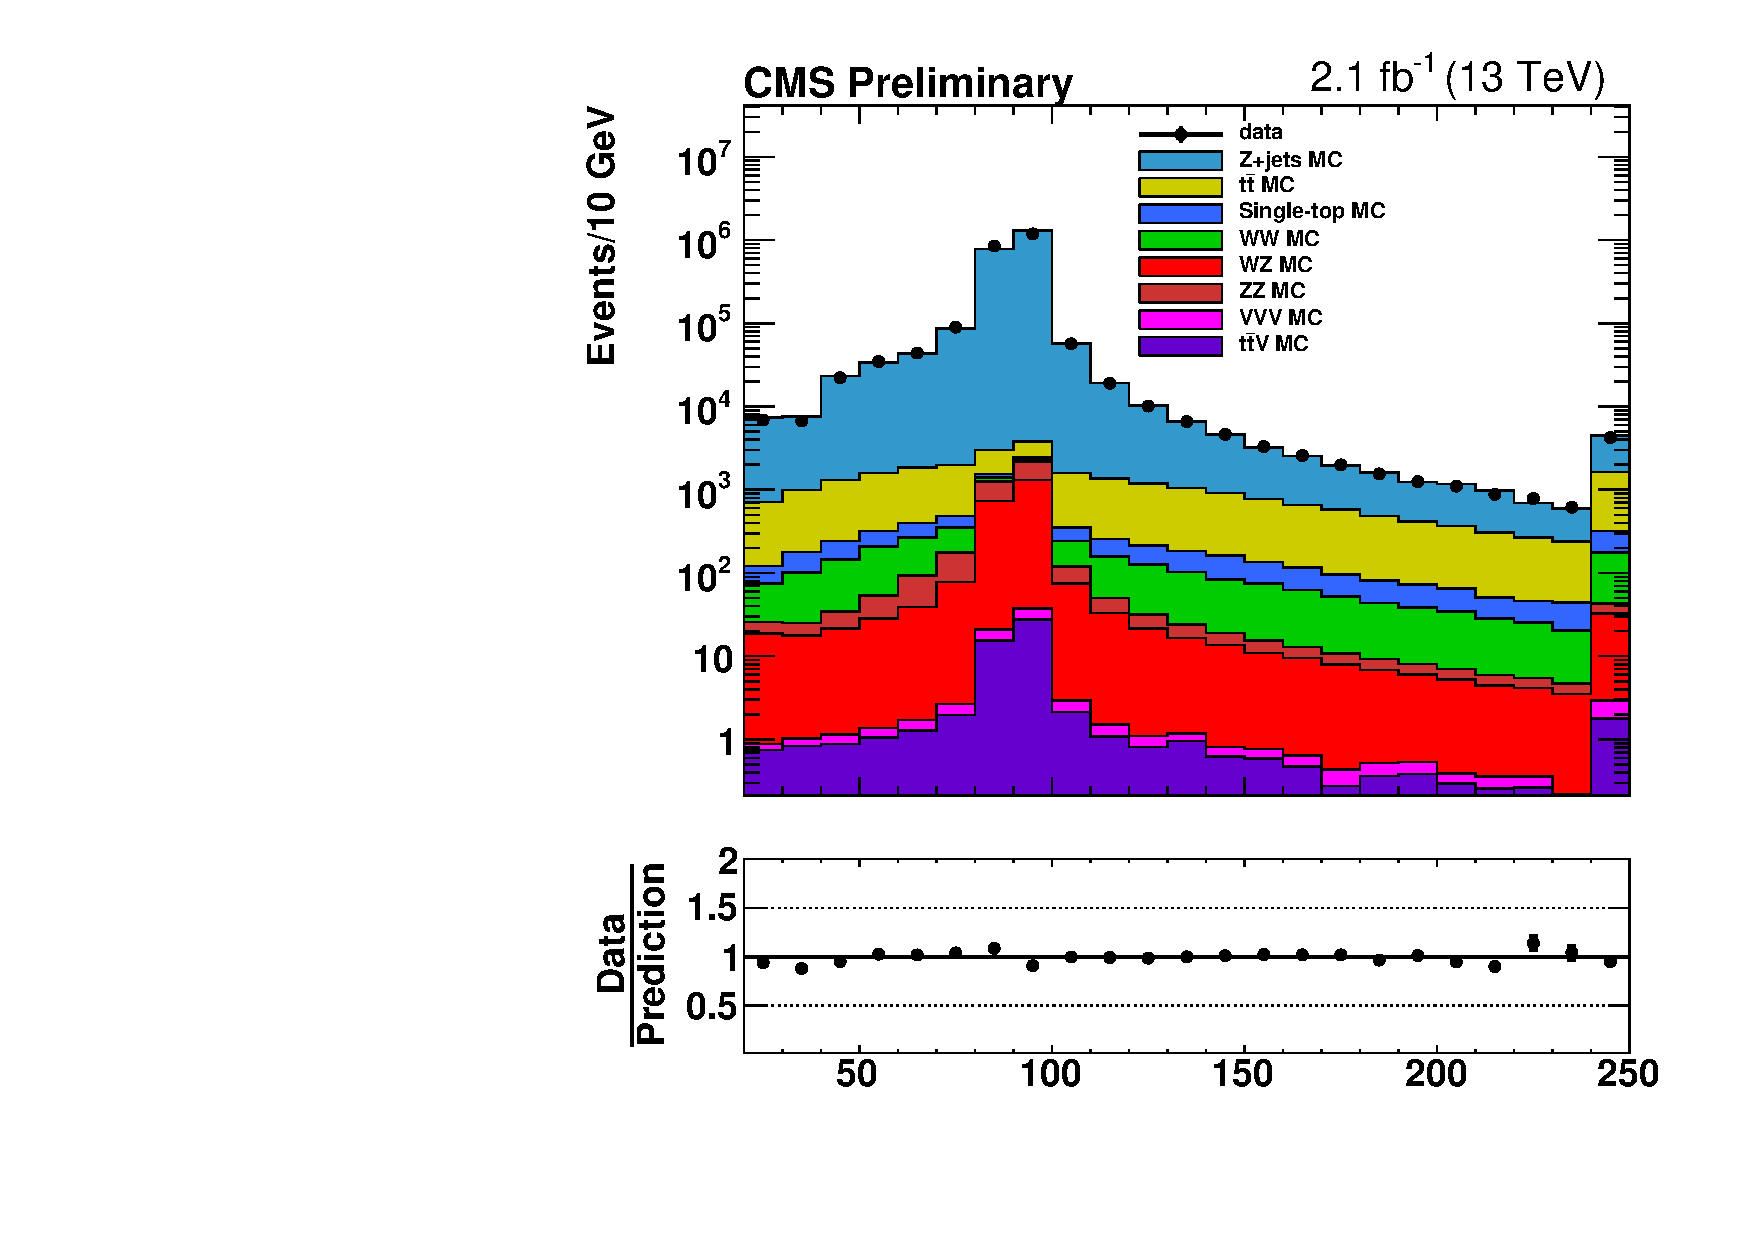
\includegraphics[width=0.4\linewidth]{evtsel/figs/h_mll_ll_signalregion_inclusive_passtrig.pdf} &
      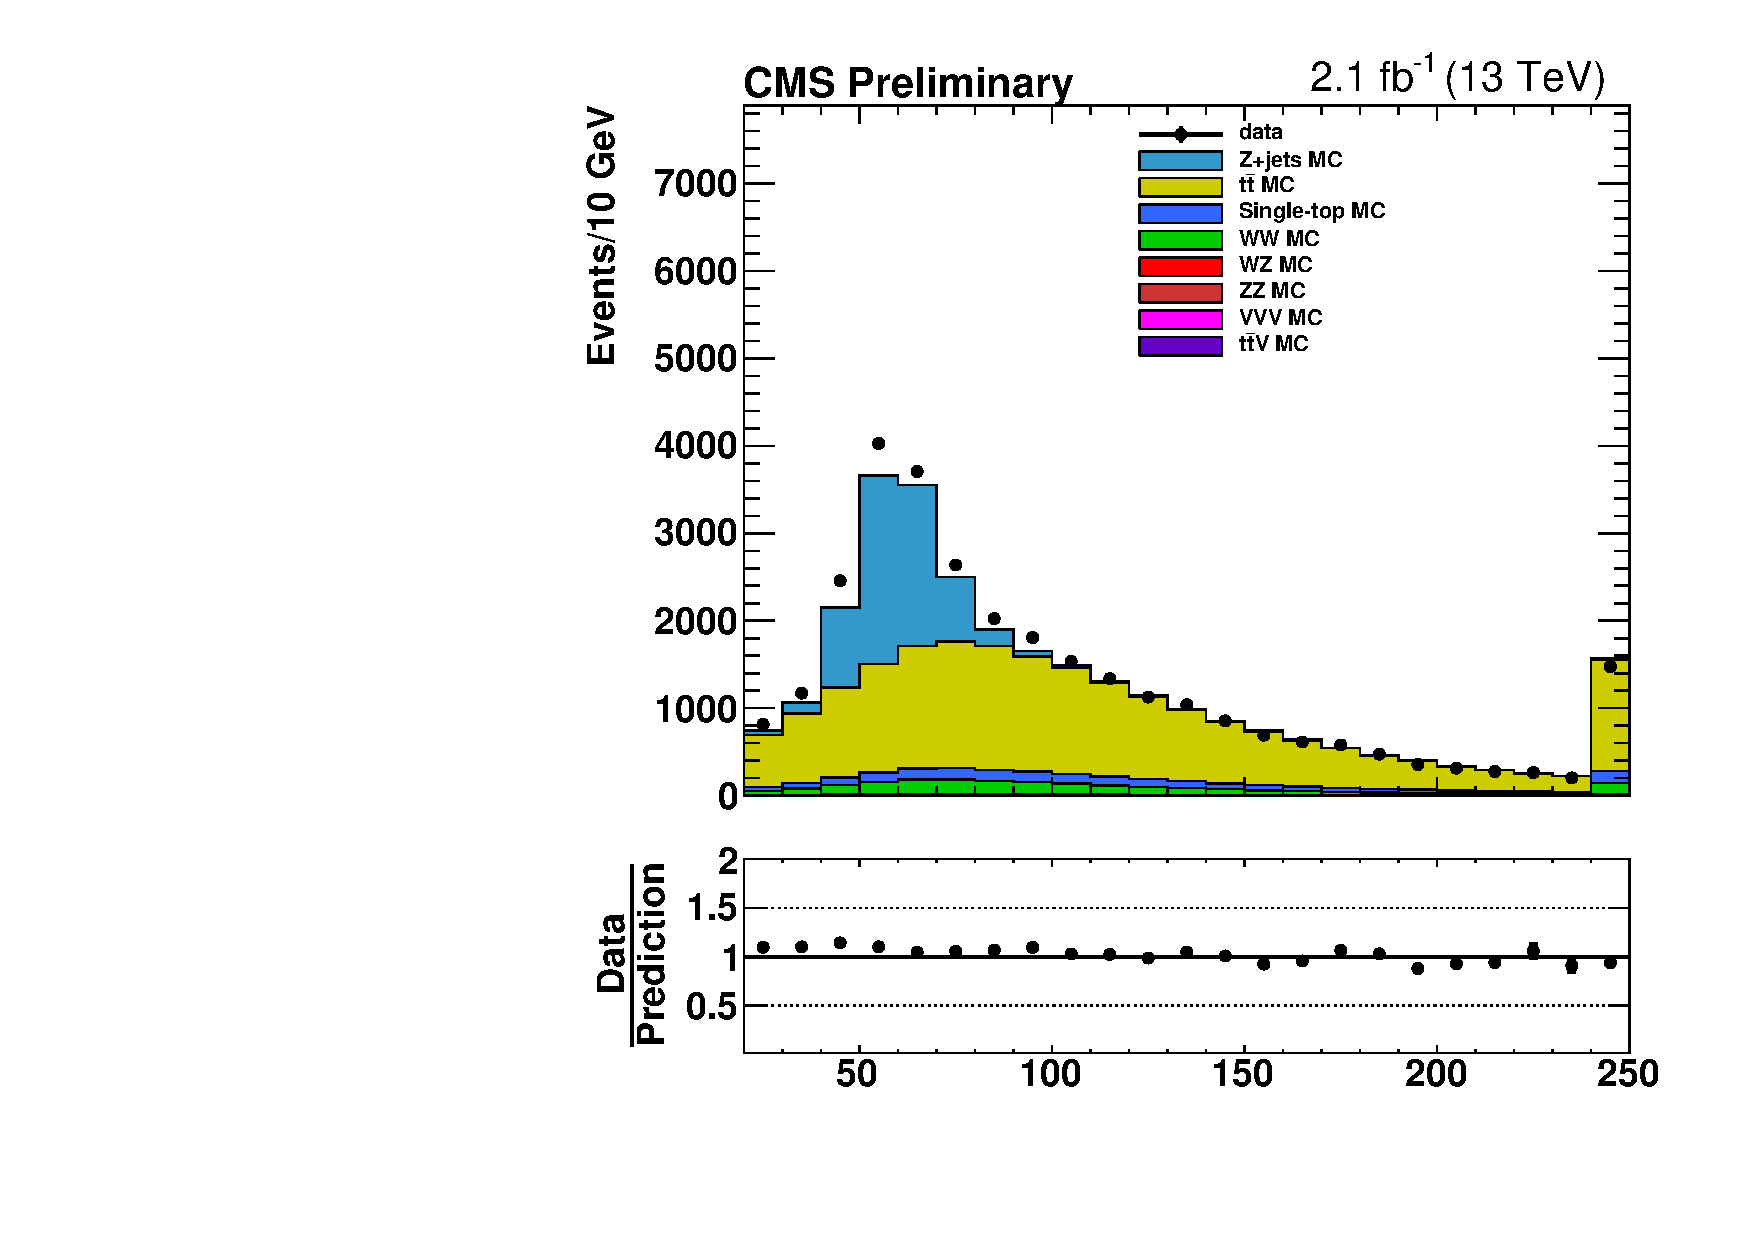
\includegraphics[width=0.4\linewidth]{evtsel/figs/h_mll_em_signalregion_inclusive_passtrig.pdf} \\
    \end{tabular}
    \caption{
      \label{fig:datavsmc_mll_emll}
      data vs. MC comparison showing \mll\ with ee+$\mu\mu$~events on the left and e$\mu$~events on the right.
    }
  \end{center}
\end{figure}

\begin{figure}[!ht]
  \begin{center}
    \begin{tabular}{cc}
      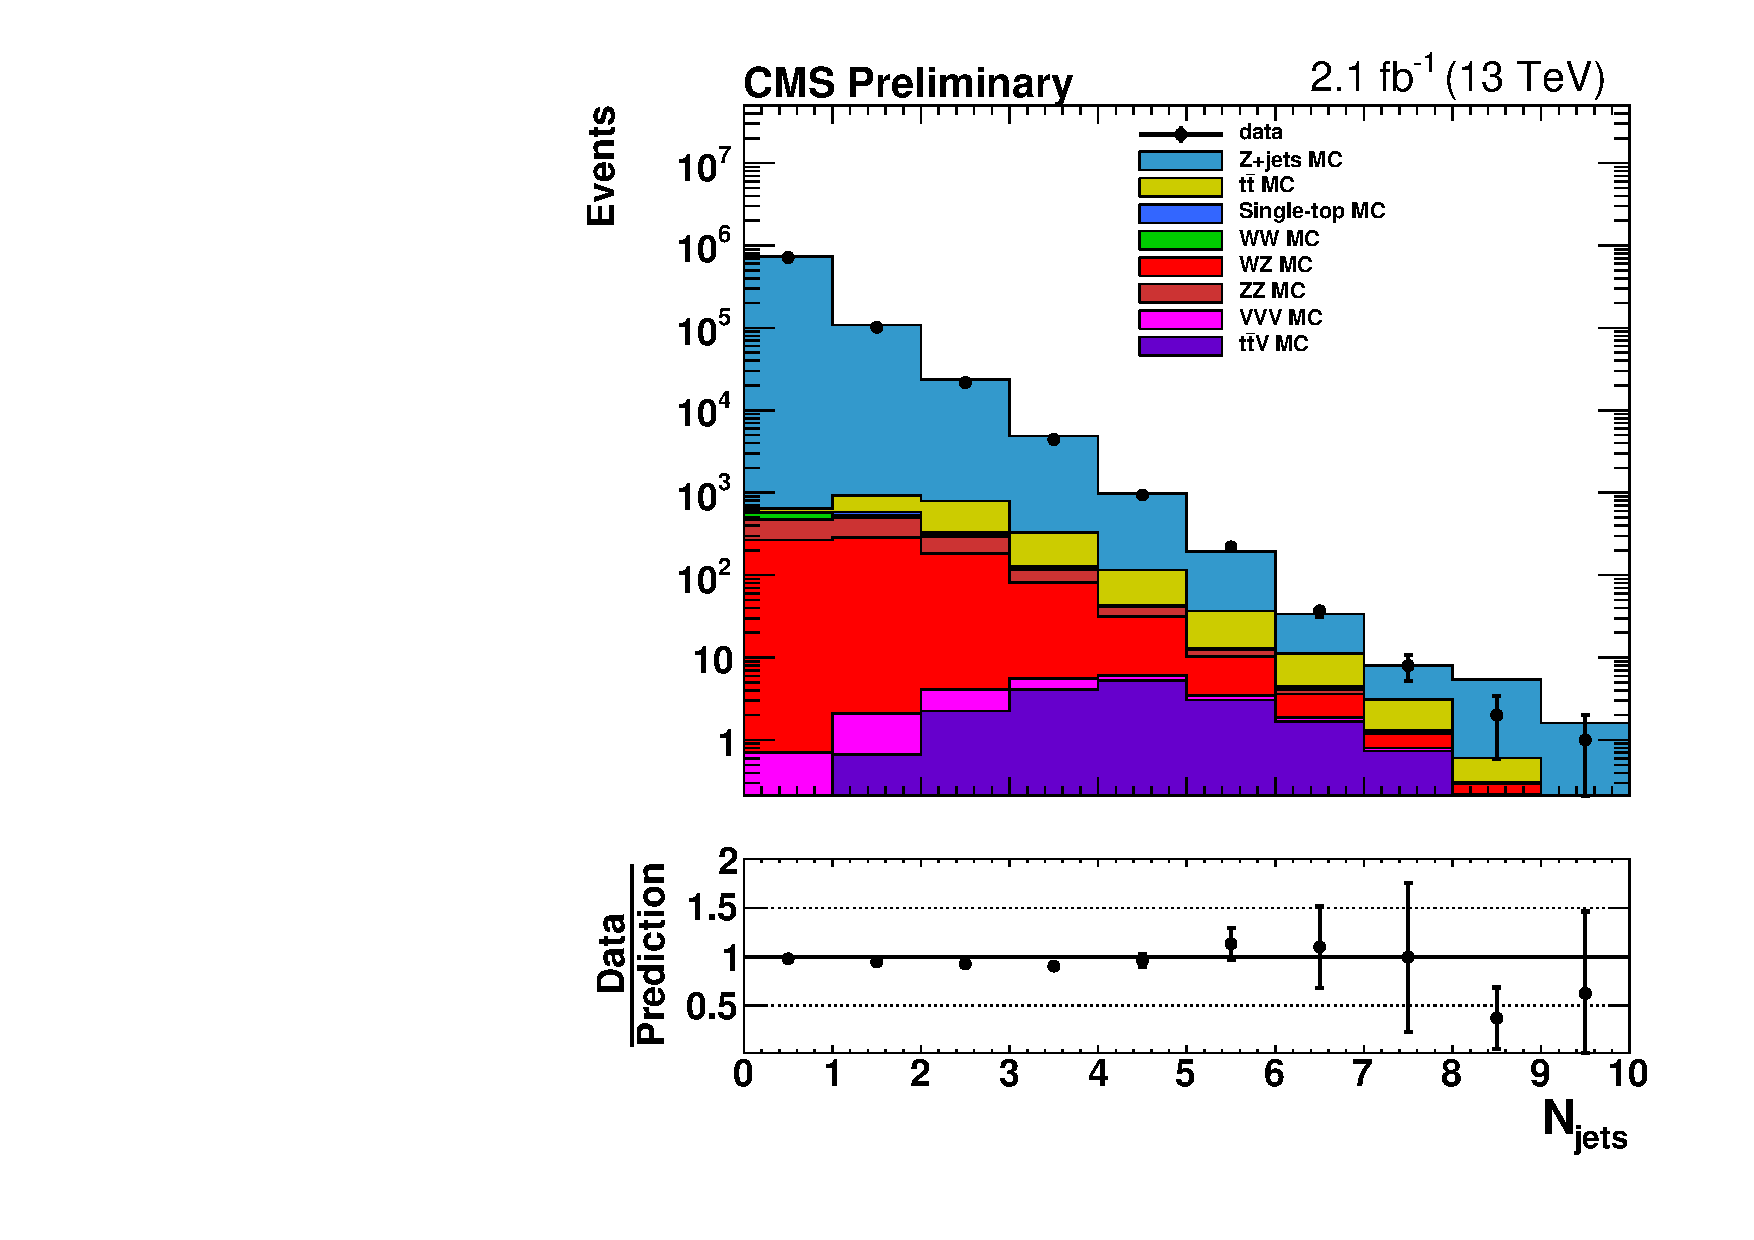
\includegraphics[width=0.4\linewidth]{evtsel/figs/h_njets_ee_signalregion_inclusive_passtrig.pdf} &
      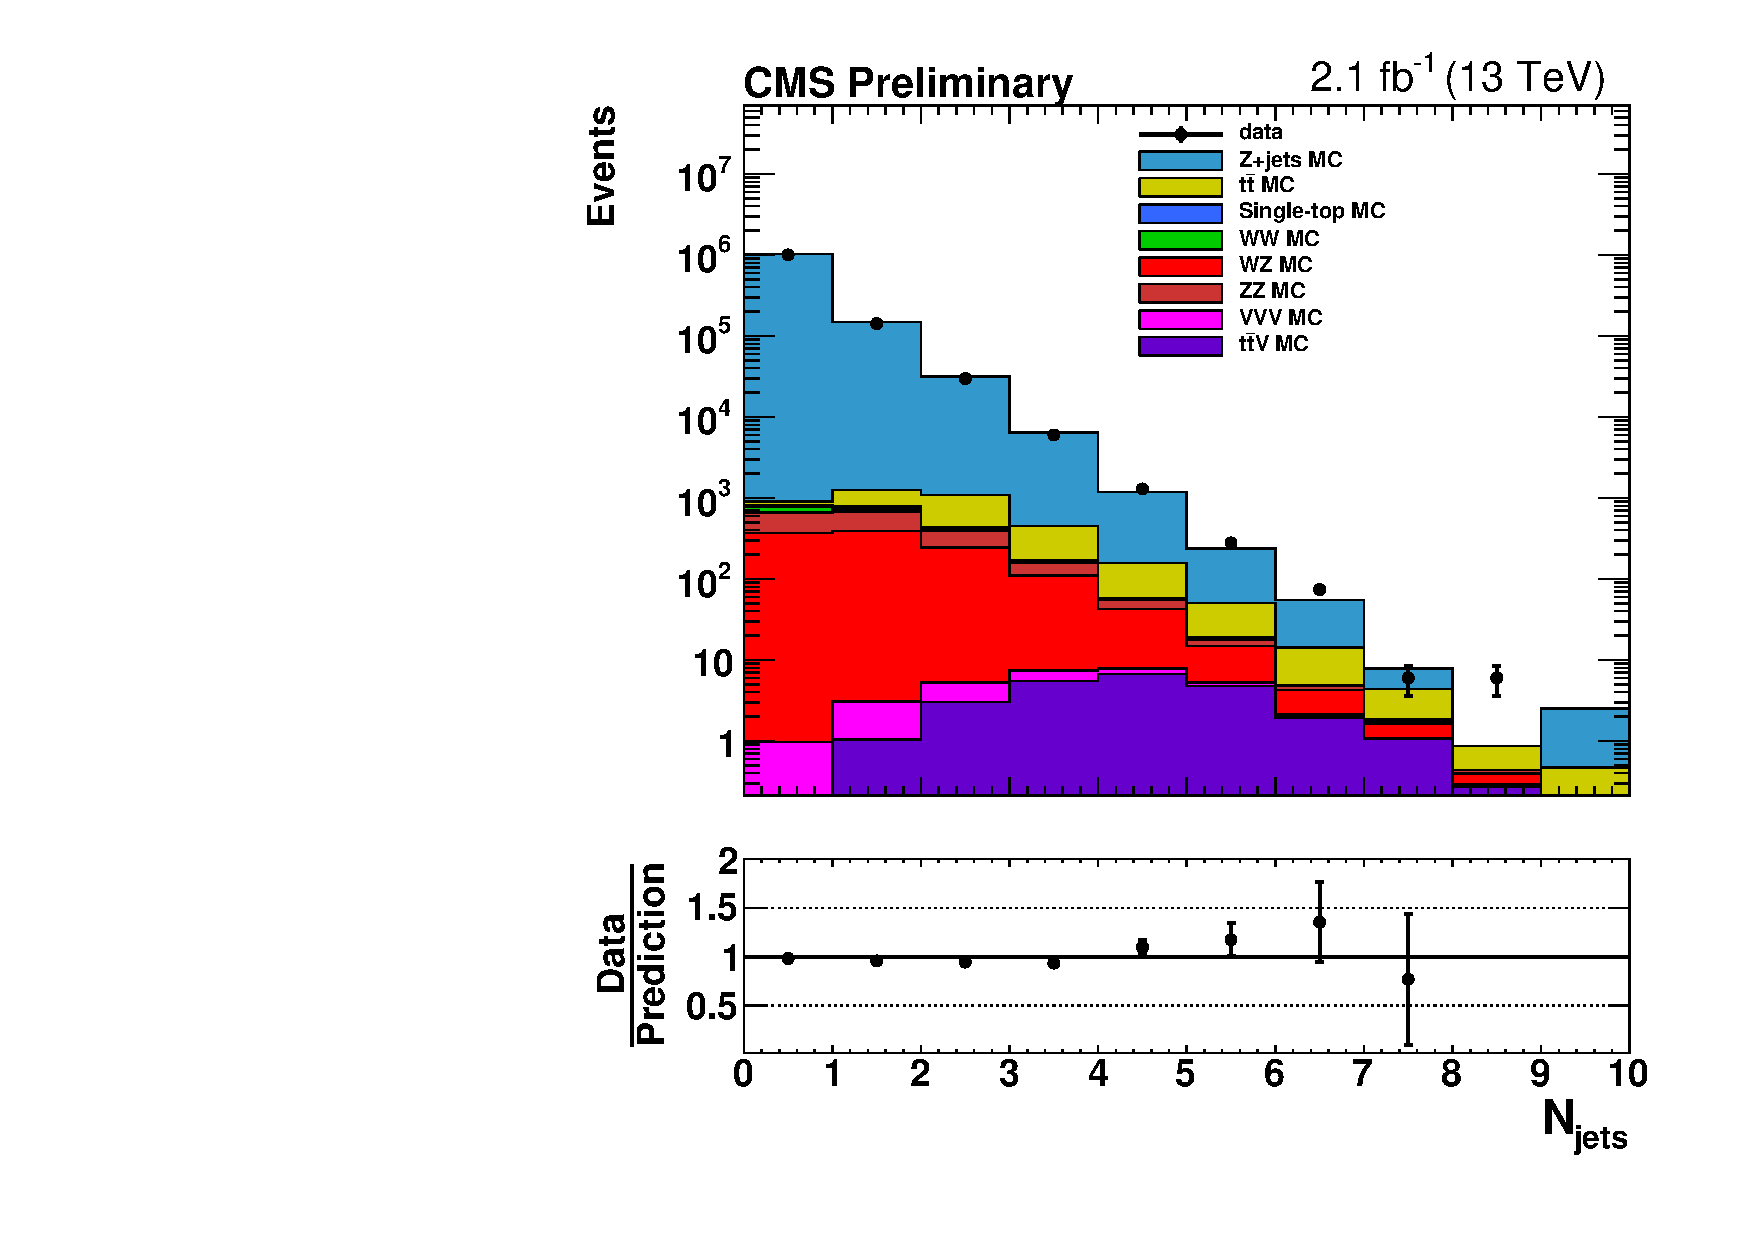
\includegraphics[width=0.4\linewidth]{evtsel/figs/h_njets_mm_signalregion_inclusive_passtrig.pdf} \\
    \end{tabular}
    \caption{
      \label{fig:datavsmc_njets}
      data vs. MC comparison showing $\mathrm{N_{jets}}$ with ee events on the left and $\mu\mu$~events on the right.
    }
  \end{center}
\end{figure}

\begin{figure}[!ht]
  \begin{center}
    \begin{tabular}{cc}
      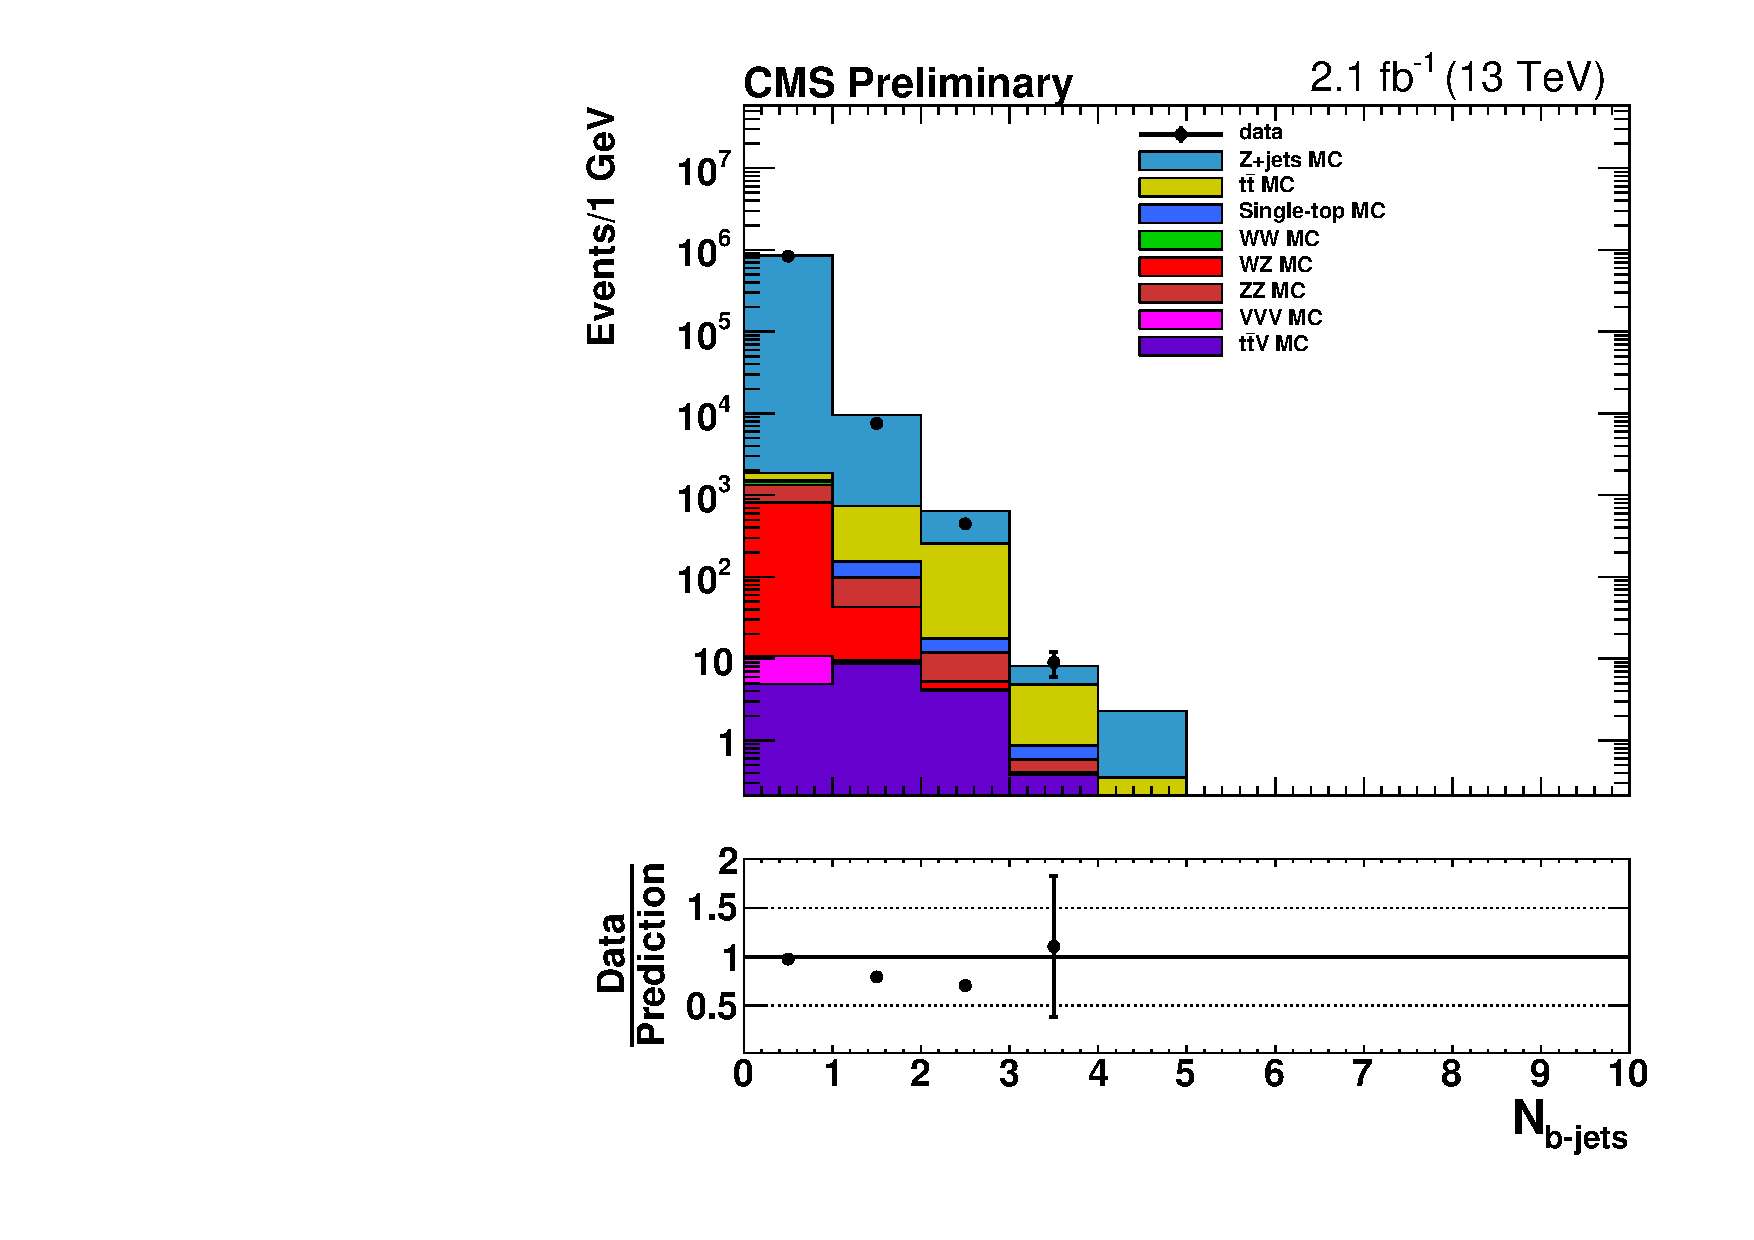
\includegraphics[width=0.4\linewidth]{evtsel/figs/h_nbjets_ee_signalregion_inclusive_passtrig.pdf} &
      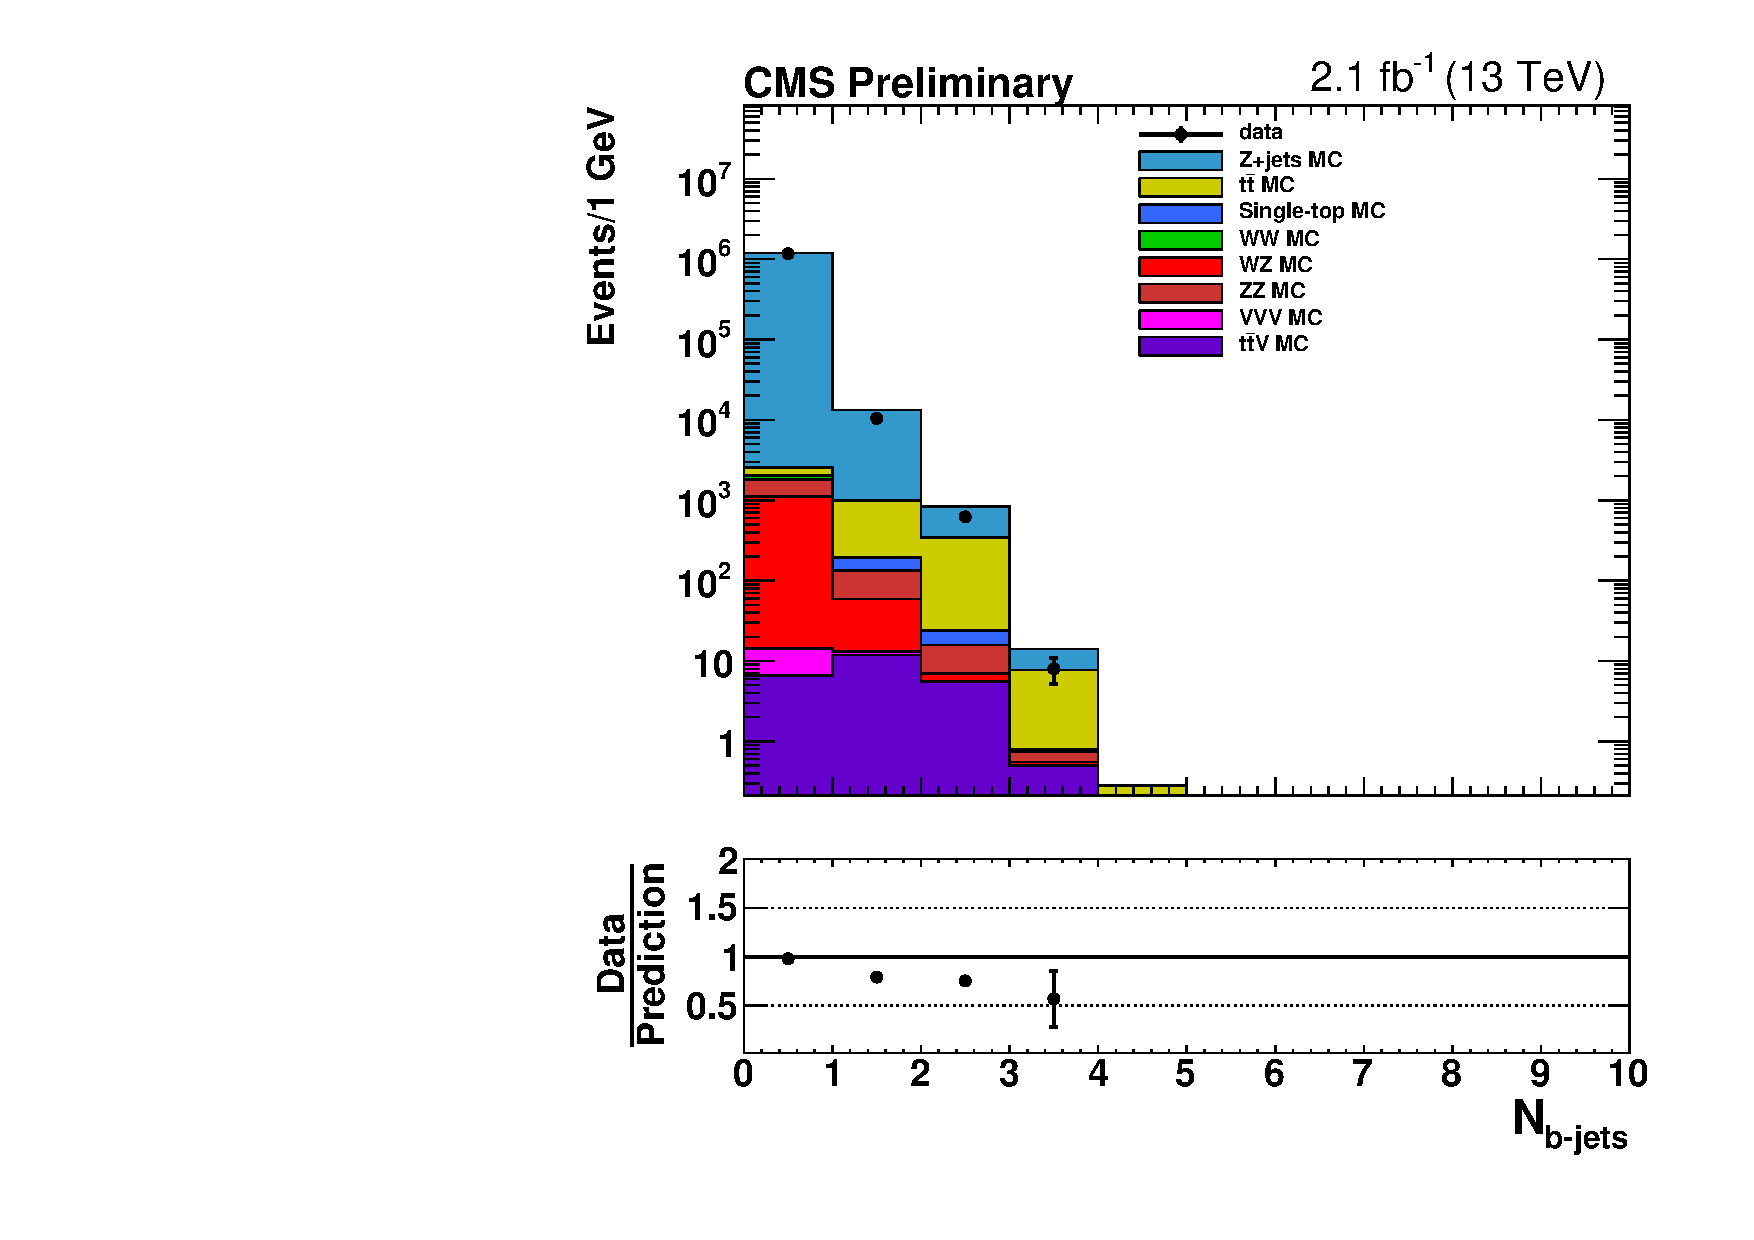
\includegraphics[width=0.4\linewidth]{evtsel/figs/h_nbjets_mm_signalregion_inclusive_passtrig.pdf} \\
    \end{tabular}
    \caption{
      \label{fig:datavsmc_nbjets}
      data vs. MC comparison showing $\mathrm{N_{b-jets}}$ with ee events on the left and $\mu\mu$~events on the right.
    }
  \end{center}
\end{figure}

\begin{figure}[!ht]
  \begin{center}
    \begin{tabular}{cc}
      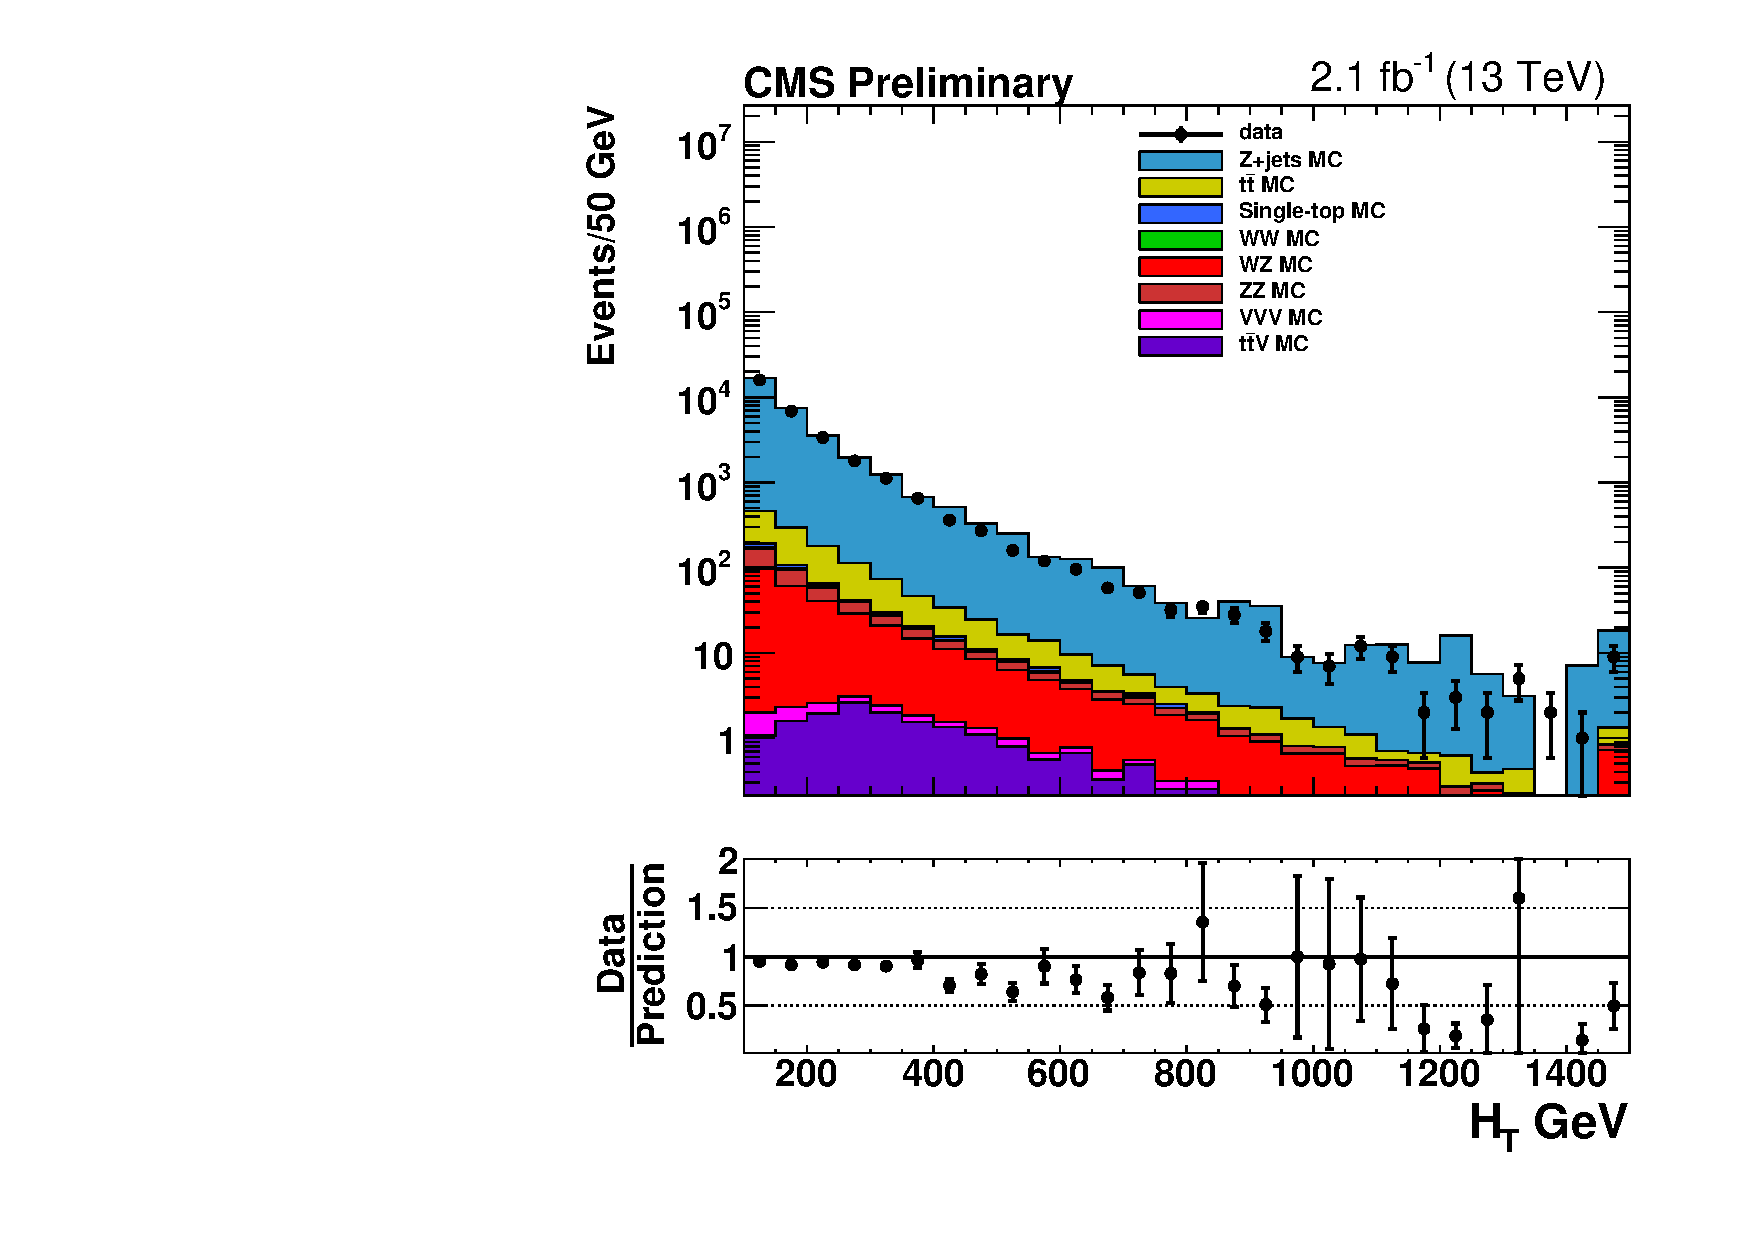
\includegraphics[width=0.4\linewidth]{evtsel/figs/h_ht_highbin_ee_signalregion_inclusive_passtrig.pdf} &
      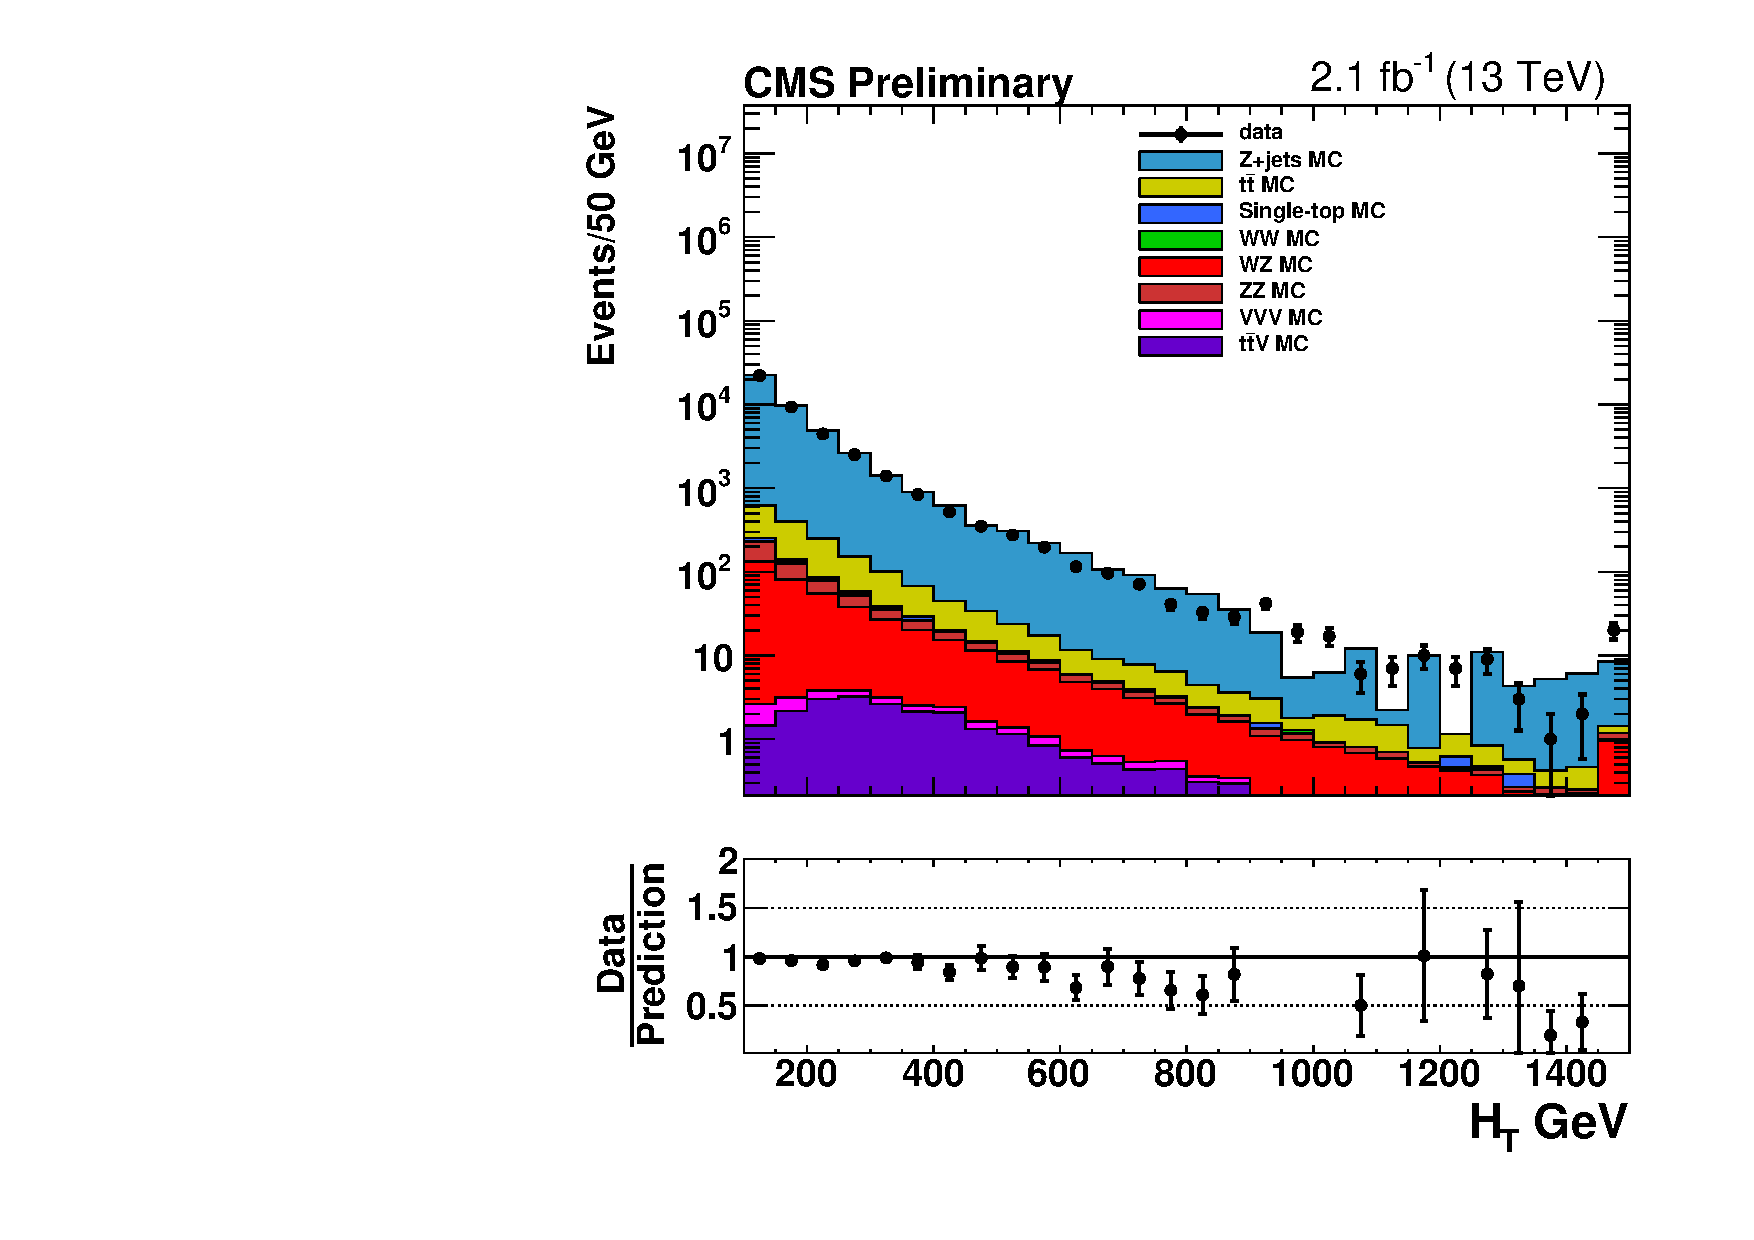
\includegraphics[width=0.4\linewidth]{evtsel/figs/h_ht_highbin_mm_signalregion_inclusive_passtrig.pdf} \\
    \end{tabular}
    \caption{
      \label{fig:datavsmc_ht}
      data vs. MC comparison showing \HT\ with ee events on the left and $\mu\mu$~events on the right.
    }
  \end{center}
\end{figure}

\begin{figure}[!ht]
  \begin{center}
    \begin{tabular}{cc}
      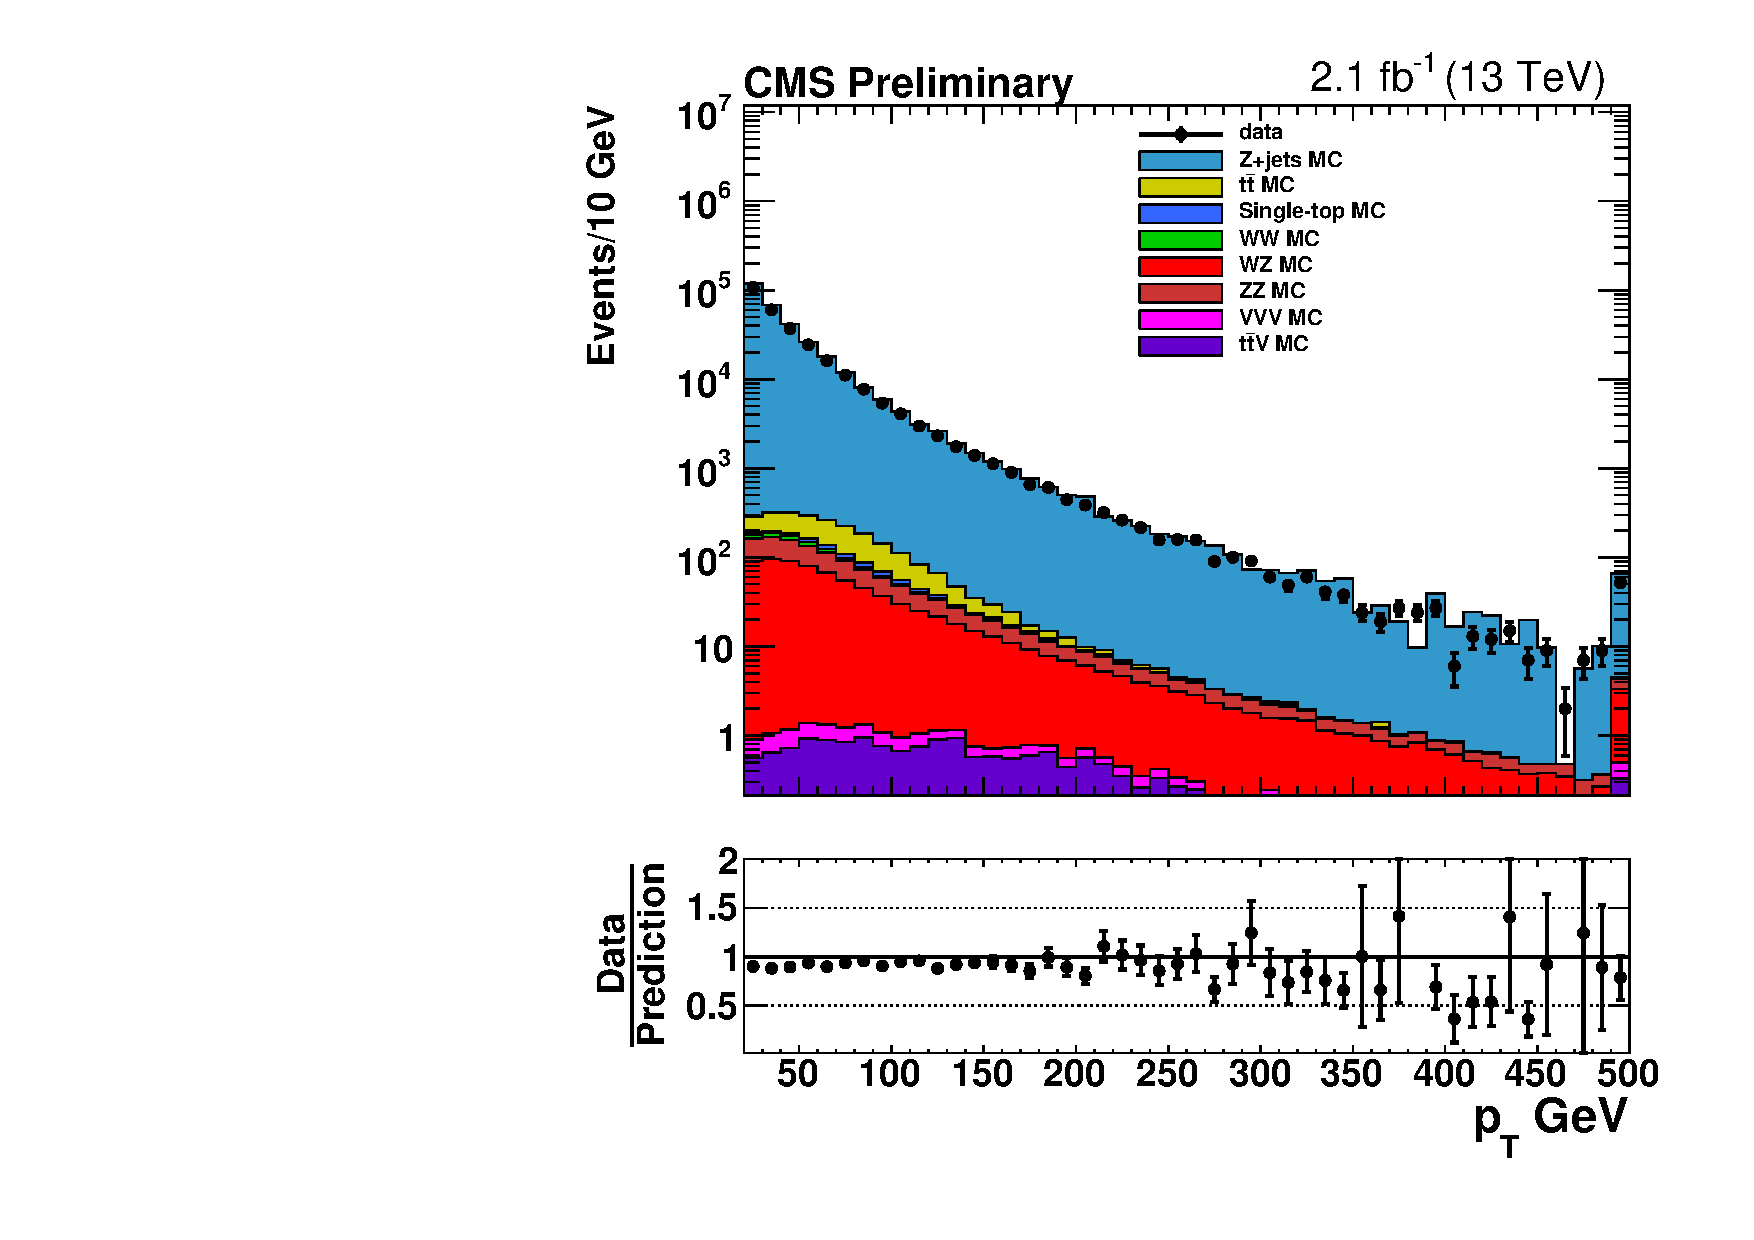
\includegraphics[width=0.4\linewidth]{evtsel/figs/h_ptdil_ee_signalregion_inclusive_passtrig.pdf} &
      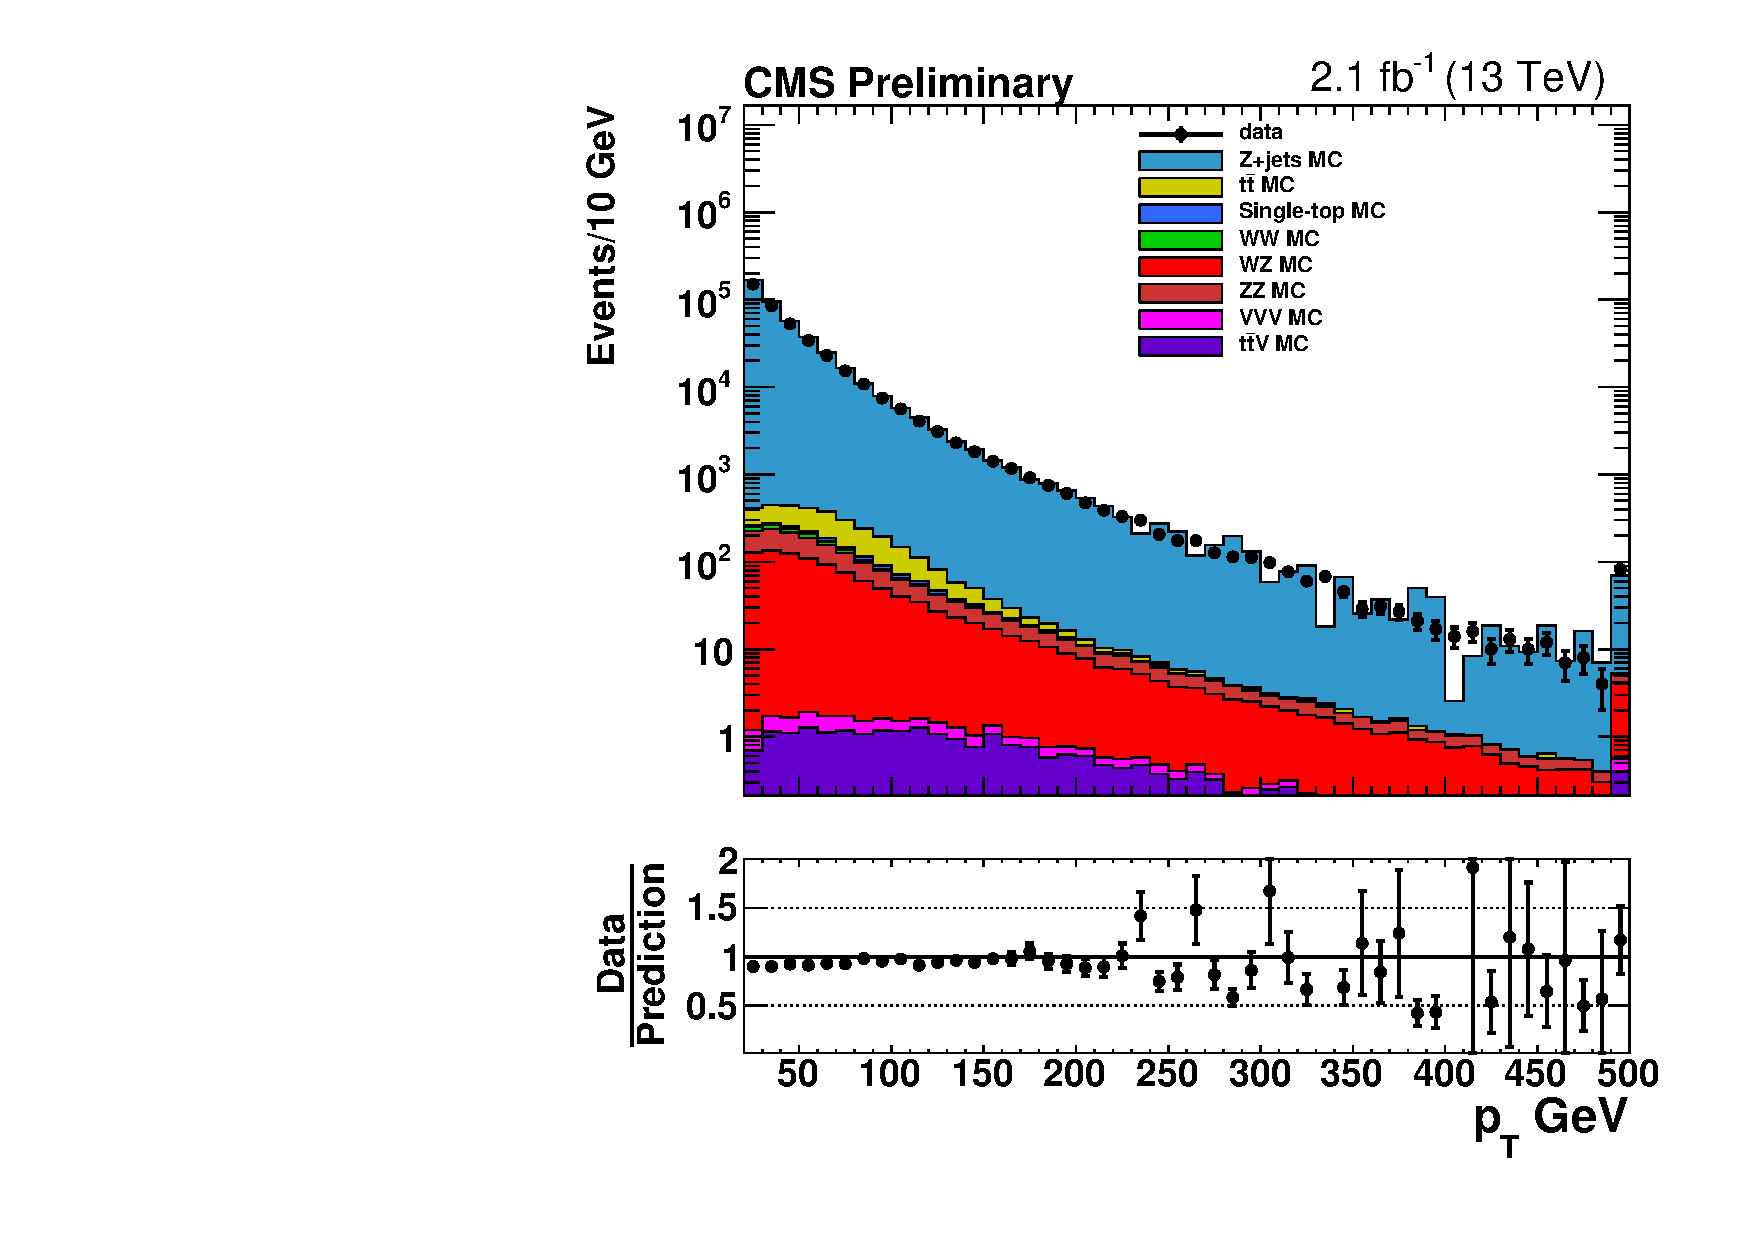
\includegraphics[width=0.4\linewidth]{evtsel/figs/h_ptdil_mm_signalregion_inclusive_passtrig.pdf} \\
    \end{tabular}
    \caption{
      \label{fig:datavsmc_ptdil}
      data vs. MC comparison showing Z \pt\ with ee events on the left and $\mu\mu$~events on the right.
    }
  \end{center}
\end{figure}

\clearpage

\section{Event Selection}
The object selections in this analysis are based on recommendations made by the relevant physics object groups (POGs) in CMS.
These groups are responsible for providing analyzers using data from the CMS experiment with a guideline of how to select specific objects in the event.
These object selections are presented to the experiment as a whole and approved before being commissioned.
In the following sections, the specific object and event selections used in this analysis are described in detail.

\subsection{Vertex Selection}
The method to choose the primary vertices in the event is described in section~\ref{ssec:vtxandpileup}.
For every event, we require the presence of at least one primary vertex satisfying the following criteria:

\begin{itemize}
\item vertex is not fake; \# of degrees of freedom($\mathrm{ndf}$)$>4$; quality requirement
\item $\rho<2$ cm \&\ $|z|<24$ cm; require vertex is inside tracker volume
\end{itemize}

$\rho$ is the radial distance from the center of the beam spot,
and $|z|$ is the distance along the beam direction calculated from the center of the beam spot.

\subsection{MET filters}
\label{ssec:metfilter}
A set of filters designated ``\MET\ filters'' are used in this analysis,
where these filters are designed to remove events in data where large values of \MET\
occur that can come from effects such as noise in the detector or the reconstruction algorithm failing.
The first of these is simply a requirement that at least one good primary vertex is reconstructed in the event.
The next filter is designed to remove events where hits are left in the CSC due to ``beam halo'' effects.
Beam halo is cause by radiation coming from the interactions with the beam in the beam pipe before the beams are collided inside the detector volume.
Additionally, a filter is appplied to deal with energy spikes in the HCAL.
These spikes come from beam halo effects where particles interact with the HCAL in a direction along the beamline leaving large energy signatures.
A filter is then applied for situations where the ECAL readout is saturated.
This happens in regions of the ECAL where there is no coverage due to bad crystals or lack of crystals.
In these regions, the trigger readout is still available but saturates above a certain energy.
When the trigger readout is saturated and the \MET\ vector aligns with an ECAL object in $\phi$, these events are removed.
The next filter applied has to do with known regions in the ECAL where the crystals were previously shown to give incorrect measurements in an inconsistent way.
When events have large energies in any of these regions aligned with \MET, the event is filtered.
The last filter has to do with muon reconstruction.
Muons are reconstructed using hits in the muon chamber and matching them with tracks in the tracker.
When a low quality muon is reconstructed,
there is a non-negligible chance for the muon to be matched incorrectly in such a way that it gives a large \pt\ value,
which then translates to large \MET.

\subsection{Lepton Selection}
\label{ssec:lepsel}
The goal of this analysis is to study events with a Z boson that decays leptonically,
and we consider only events with Z$\rightarrow\ell\ell$, where $\mathrm{\ell=e~or~\mu}$.
$\tau$s are not considered for reasons described in~\ref{ssec:lepsandphots}.
In order to select events with this decay,
it is required there be at least two leptons passing the ID and isolation requirements described below,
and that these leptons form a opposite-sign same-flavor (OSSF) pair with \mll\ between 81-101 \gev.
When more than one good OSSF di-lepton pair passes all the lepton requirements,
the pair consisting of the two highest \pt\ leptons is chosen.
The two highest \pt\ leptons in the event are required to have \pt\ $> 20$ \gev.
This requirement is chosen based on the expected di-lepton trigger \pt\ thresholds.
In order to have high precision when identifying and reconstructing leptons,
the leptons are required to be contained within the tracker volume.
This is done by requiring both leptons to have $|\eta| < 2.4$.
In order to avoid the transition region from the endcap to the barrel, 
where the muon and electron reconstruction efficiencies are very different, 
leptons having $|\eta|$ in the range 1.4 $< |\eta| <$ 1.6 are rejected.
Events are vetoed if the two leading leptons are within a cone of $\Delta R < 0.1$ from each other,
in order to reduce the rate of events with fake leptons.
These selections are summarized below.

\begin{itemize}
\item Require two leading leptons to be opposite-sign same-flavor (OSSF) ee and $\mu\mu$ pairs
\item The dilepton invariant mass is required to be consistent with the Z mass; namely $81<m_{\ell\ell}<101$~\gev
\item \pt\ $> 20$ \gev\ for the two leptons making up the di-lepton pair
\item $|\eta| < 1.4$~or $1.6 < |\eta| < 2.4$~for the two leptons making up the di-lepton pair
\item $\Delta R$~between the two leading leptons must be greater than 0.1
\end{itemize}

\subsection{Lepton Isolation}
\label{ssec:isolation}
The signal region targeted by this analysis is expected to have large \HT\ due to the many jets in the final state.
This leads to an increased probability of a lepton overlapping with a jet in the event.
When this happens, the lepton is no longer isolated and may fail a cut on the raw isolation value.
The isolation variable is designed to reduce this inefficiency by using a variable cone size that depends on lepton \pt.
For leptons with \pt\ $<$~50 \gev, we use a cone with $\Delta\mathrm{R = 0.2}$,
for leptons with \pt: 50 - 200 \gev, we use a variable cone defined as $\Delta\mathrm{R = \frac{10}{p_{T}(lep)}}$,
and for leptons with \pt $>$~200 \gev, we use a cone with $\Delta\mathrm{R = 0.05}$.
Isolation is calculated according to equation~\ref{eqn:isolation},
where $\mathrm{p_{T}(i)}$~represents all the pf candidates within the cone defined above.
When cutting on isolation, the value is chosen relative to $\mathrm{p_{T}(lepton)}$. 
This quantity is designated mini-relative Isolation (miniRelIso).

\begin{equation}
\label{eqn:isolation}
\mathrm{I_{lepton}} = \sum _{i} |\mathrm{p_{T}(i)| - |p_{T}(lepton)}|
\end{equation}

Before cutting on isolation,
corrections are made to account for pileup energy using the effective area $\rho$ corrections scheme.
In this scheme, $\rho$ is the total energy density from pileup and is assumed to be uniform in the detector.
The correction to isolation is done by calculating the energy from pileup in the isolation cone and subtracting it from the total energy in the cone.

This correction is not derived using the geometric area of the cone however
due to the fact that the response of $I_{lepton}$ and $\rho$ are different with respect to the amount of pileup.
Instead, the geometric area of each lepton's isolation cone is scaled in separate regions of $\eta$
by a factor derived using the number of primary vertices in the event as a way to estimate the amount of pileup.
These factors are derived separately for electrons and muons and shown in tables~\ref{tab:eamus}~and~\ref{tab:eaels}.

\begin{table}[htb]
\begin{center}
  \caption{
    \label{tab:eamus}
    Effective area values for muons derived in separate regions of $\eta$ are shown in this table.
  }
\begin{tabular}{l|c}
\hline
\hline
$\eta$~region        & Muon effective area \\
\hline
$|\eta| < 0.8$       & 0.0735 \\
0.8$ < |\eta| < $1.3 & 0.0619 \\
1.3$ < |\eta| < $2.0 & 0.0465 \\
2.0$ < |\eta| < $2.2 & 0.0433 \\
2.2$ < |\eta| < $2.5 & 0.0577 \\
\hline
\hline
\end{tabular}
\end{center}
\end{table}

\begin{table}[htb]
\begin{center}
  \caption{
    \label{tab:eaels}
    Effective area values for electrons derived in separate regions of $\eta$ are shown in this table.
  }
\begin{tabular}{l|c}
\hline
\hline
$\eta$~region          & Electron effective area \\
\hline
$|\eta| < 1.0$         & 0.1752 \\
1.0$ < |\eta| < $1.3   & 0.1862 \\
1.479$ < |\eta| < $2.0 & 0.1411 \\
2.0$ < |\eta| < $2.2   & 0.1534 \\
2.2$ < |\eta| < $2.3   & 0.1903 \\
2.3$ < |\eta| < $2.4   & 0.2243 \\
2.4$ < |\eta| < $2.5   & 0.2687 \\
\hline
\hline
\end{tabular}
\end{center}
\end{table}

The effective area is then defined by equation~\ref{eqn:effarea} where f is the scale factor, and R is the cone size defined above.

\begin{equation}
\label{eqn:effarea}
\mathrm{A_{eff} = f*\pi * R^2}
\end{equation}

The plots in figures~\ref{fig:isoels}~and~\ref{fig:isomus}
show the isolation distribution for leptons that pass the ID selections made using simulated \zjets\ MC.
These leptons are separated into two categories, prompt and non-prompt leptons.
Prompt leptons are defined to be leptons that come directly from the hard scatter process rather than a second order process, for example semi-leptonic b-decay.
In order to study the difference in expected behavior of prompt and non-prompt leptons, a disctinction is made such that a prompt,
reconstructed lepton is defined as being matched to a generator-level lepton within a cone of $\Delta$R < 0.4.
Any lepton that passes the ID requirements that does not pass this matching requirement is designated as a non-prompt lepton.

\begin{figure}[!ht]
\begin{center}
\begin{tabular}{cc}
\includegraphics[width=0.4\textwidth]{evtsel/figs/EA_iso_el.pdf} & 
\includegraphics[width=0.4\textwidth]{evtsel/figs/EA_iso_el_inclusive.pdf} \\
\end{tabular}
\caption{
  The isolation distribution is shown for electrons on the left in simulated \zjets\ MC events.
  On the right, the efficiency is shown when integrating all bins to the left of the value on the x-axis.
\label{fig:isoels}
}
\end{center}
\end{figure}

\begin{figure}[!ht]
\begin{center}
\begin{tabular}{cc}
\includegraphics[width=0.4\textwidth]{evtsel/figs/EA_iso_mu.pdf} & 
\includegraphics[width=0.4\textwidth]{evtsel/figs/EA_iso_mu_inclusive.pdf} \\
\end{tabular}
\caption{
  The isolation distribution is shown for muons on the left in simulated \zjets\ MC events.
  On the right, the efficiency is shown when integrating all bins to the left of the value on the x-axis.
\label{fig:isomus}
}
\end{center}
\end{figure}

After applying the effective area corrections,
the leptons in this analysis are required to have miniRelIso $<$ 0.10 ( 0.20) for electrons (muons). 
This gives an efficiency for prompt leptons of $>$~90\% and rejection rate for non-prompt leptons of about 80\% for electrons and 90\% for muons.
\clearpage

\subsection{Lepton Scale Factors}
\label{ssec:lepscalefactors}
Scale factors are applied in order to correct for the differences in efficiencies in data and MC when applying lepton ID and isolation requirements.
Additional scale factors are derived to correct for differences in simulation of leptons when using Fastsim~\cite{fastsim} instead of fullsim.
These scale factors are derived in data and MC using a ``tag and probe'' technique.
The main premise of this technique is that leptons coming from a Z boson are produced in opposite-sign same-flavor pairs in very large quantities.
In an event, a lepton with very tight ID and isolation requirements is chosen (the tag),
and then a second lepton with very loose requirements (the probe) can be studied if it is found that the pair of leptons has a dilepton mass consistent with the Z mass.
The efficiency of various cut requirements is then assessed for individual leptons, such as the efficiency of the ID and isolation requirements.
This is done separately in data and MC, and then the MC is corrected based on these differences to match what is observed in data.
Scale factors for electron ID and isolation criteria are shown in~\ref{fig:sf_electrons},
scale factors for muon ID and isolation criteria are shown in~\ref{fig:sf_muons},
and Fastsim scale factors are shown in~\ref{fig:FS_sfs}.
\begin{figure}[!ht]
  \begin{center}
      \includegraphics[width=0.8\textwidth]{evtsel/figs/sf_el_tight2d3d.pdf}  
    \caption{
      \label{fig:sf_electrons}
      Electron scale factors as a function of \pt\ and $\eta$.
      The scale factor is applied as an event weight once per electron in the event.
    }
  \end{center}
\end{figure}

\begin{figure}[!ht]
  \begin{center}
    \begin{tabular}{cc}
      \includegraphics[width=0.4\textwidth]{evtsel/figs/sf_mu_mediumID.pdf}  &
      \includegraphics[width=0.4\textwidth]{evtsel/figs/sf_mu_mini02.pdf}  \\
    \end{tabular}
    \caption{
      \label{fig:sf_muons}
      Muon scale factors as a function of \pt\ and $\eta$.
      The left plot shows the scale factors associated with the ID selection criteria,
      and the right plot shows the scale factors associated with the isolation selection criteria.
      Each scale factor is applied as an event weight once per muon in the event.
    }
  \end{center}
\end{figure}

\begin{figure}[!ht]
  \begin{center}
    \begin{tabular}{cc}
      \includegraphics[width=0.4\textwidth]{evtsel/figs/FS_sf_el_tight_mini01.pdf}  &
      \includegraphics[width=0.4\textwidth]{evtsel/figs/FS_sf_mu_mediumID_mini02.pdf}  \\
    \end{tabular}
    \caption{
      \label{fig:FS_sfs}
      Fastsim scale factors as a function of \pt\ and $\eta$.
      The left plot shows the scale factors applied per electron,
      and the right plot shows the scale factors applied per muon.
      Each scale factor is applied as an event weight once per lepton in the event.
    }
  \end{center}
\end{figure}

\clearpage

\subsection{Electron Selection}
\label{ssec:elsel}
Output from a multivariate analysis (MVA) is used to identify the electrons used in this analysis~\cite{egamma13tev} based on a method used previously~\cite{egamma8tev}.
This is done separately in the barrel and endcap using a variety of kinematic variables as input.
Electrons with \pt $>$ 15 GeV and $|\eta|<2.4$ are considered.
The training of the MVA is done using a Z+jets MC sample where the electrons used as signal input are
required to be matched to generator level electrons, and electrons used as background are required to not be matched.

Variables used to differentiate electrons from fakes mainly use information from the tracker and ECAL.
Measurements made by the ECAL and tracker are compared using the ratio of the electron cluster energy to the track momentum at the outermost track layer.
This ratio is expected to be 1 for real electrons, but not necessarily for fakes.
$\sigma_{i\eta i\eta}$ is a purely calorimetric variable which uses the shower shape of the electron object to differentiate real and fake electrons.
The main premise behind this variable is that electron energies are contained within 1-2 crystals in $\eta$
where ECAL energy from charged hadrons is spread across many crystals leading to the shape for real electrons and fake electrons to be very different making it a good variable to differentiate the two.
A way to differentiate real and fake electrons is to check the consistency of the track of the reconstructed electron object left in the tracker.
This is done by measuring the difference in $\eta$ of the track measured in the outer layer and the electron cluster in the ECAL ($\mathrm{\Delta\eta(track-cluster)}$).
An plot showing how each of these variables looks for real and fake electrons is shown in figure~\ref{fig:electron_mva_vars},
and the output of the MVA variable in figure~\ref{fig:electron_mva_output}.

\begin{figure}[!htb]
  \begin{center}
    \begin{tabular}{cc}
      \includegraphics[width=0.4\textwidth]{evtsel/figs/EoPout_EB_LowPt.pdf} &
      \includegraphics[width=0.4\textwidth]{evtsel/figs/EoPout_EE_LowPt.pdf} \\      
      \includegraphics[width=0.4\textwidth]{evtsel/figs/deltaEta_EB_LowPt.pdf} &
      \includegraphics[width=0.4\textwidth]{evtsel/figs/deltaEta_EE_LowPt.pdf} \\      
      \includegraphics[width=0.4\textwidth]{evtsel/figs/see_EB_LowPt.pdf} &
      \includegraphics[width=0.4\textwidth]{evtsel/figs/see_EE_LowPt.pdf} \\      
    \end{tabular}
    \caption{
      \label{fig:electron_mva_vars}
      Kinematic variables used to distinguish real electrons from fake electrons are shown
      with electrons in the barrel on the left and electrons in the endcap on the right.
    }
  \end{center}
\end{figure}
  
\begin{figure}[!htb]
  \begin{center}
    \begin{tabular}{cc}
      \includegraphics[width=0.4\textwidth]{evtsel/figs/MVA_output_EB.pdf} &
      \includegraphics[width=0.4\textwidth]{evtsel/figs/MVA_output_EE.pdf} \\      
    \end{tabular}
    \caption{
      \label{fig:electron_mva_output}
      The output of the electron MVA is shown comparing the distributions of electrons matched
      with generator level electrons (blue) vs. jets that fake electrons.
      The output in the barrel is shown in the left and endcap on the right.
    }
  \end{center}
\end{figure}
  
Electrons in data are compared to the electrons from MC using the probe leg from a
``tag and probe'' technique similar to the one described in section~\ref{ssec:lepscalefactors}.
The requirements for the probe electron are as follows:
\begin{itemize}
\item $\mathrm{p_{T}(e) > 10~GeV}$
\item $\mathrm{\eta(e) < 2.5}$
\item Loose identification criteria
\item Relative isolation (pileup corrected) < 0.1
\end{itemize}
The output of this MVA is shown in figure~\ref{fig:electron_mva},
and the MVA cut requirement for this analysis is shown in table~\ref{table:electrons}.
  
\begin{figure}[!ht]
  \begin{center}
      \includegraphics[width=0.8\textwidth]{evtsel/figs/Electron_MVA_2015.pdf}
    \caption{
      \label{fig:electron_mva}
      Output of the electron MVA is shown comparing electrons in data vs. MC with electrons in the barrel on the left and the endcap on the right.
      The electrons shown are the probe leg when using a ``Tag and Probe'' technique.
    }
  \end{center}
\end{figure}
  
\begin{table}[!htb]
  \begin{center}
    \caption{
      \label{table:electrons}
      All the requirements for electrons with \pt\ $>$ 10 \gev are shown in the table below.
      The electrons in the signal region are required to have \pt\ $>$ 20 \gev.
    }
    \begin{tabular}{l|cc}
      \hline
      Region                & MVA minimum cut value \\
      \hline
      Barrel $|\eta| < 0.8$ & 0.913286 \\
      Barrel $|\eta| > 0.8$ & 0.805013 \\
      Endcap                & 0.358969 \\
      \hline
      \hline
      Cut variable                  & Requirement   \\
      \hline
      $d_{0}$ (w.r.t. 1st good PV)   & $<0.05$ cm  \\
      $d_{z}$ (w.r.t. 1st good PV)   & $<0.1$  cm  \\
      miniRelIso / \pt              &  $<0.10$ \\
      \hline
    \end{tabular}
  \end{center}
\end{table}

The efficiency of the electron selection is measured to be on average 80\% for electrons with $\mathrm{p_{T} >~ 20~GeV}$ as seen in figure~\ref{fig:electronideff}.

\begin{figure}[!ht]
  \begin{center}
      \includegraphics[width=0.8\textwidth]{evtsel/figs/Electron_MVA_efficiency.pdf}
    \caption{
      \label{fig:electronideff}
      Electron identification efficiency in data (top) and data to MC efficiency ratios (bottom)
      measured for the identification criteria based on a MVA discriminant with an average efficiency of 80\%.
      The efficiency is measured with the tag and probe method and shown in three pseudorapidity ranges as a function of the electron transverse momentum.
    }
  \end{center}
\end{figure}
  

\subsection{Muon Selection}
\label{ssec:musel}
The muon selection criteria are based on studies performed by the muon POG at CMS~\cite{tdr1}\cite{muonReco}.
Muons with \pt $>$ 15 GeV and $|\eta|<2.4$ are considered. 
The baseline muon selection requires that the muon be identified as a muon by the particle flow algorithm,
as well as being identified as a tracker or global muon.
To define a tracker muon, all tracks in the tracker with \pt $>$~0.5 \gev\ and $p~>~2.5$~\gev are considered.
These tracks are extrapolated to the muon system and then required to have a matching segment in at least one muon station.
Global muons are defined by matching a tracker track with that of a track reconstructed independently by the muon system.
After the two tracks are matched, a global muon track fit is done combining the hits from the two separate tracks.
Muons in this analysis must either qualify as a global muon or pass a segment compatibility requirement.
Segment compatibility is defined using a template based on simulation.
In addition to these requirements, muons are required to be within 0.05 cm of the primary vertex in the x-y direction and within 0.1 cm in the z direction.
The full muon selection requirements are listed in Table~\ref{tab:muons}.

\begin{table}[htb]
\begin{center}
\caption{\label{tab:muons} A summary of the muons selection requirements is shown in this table for all muons used in this analysis.}
\begin{tabular}{l|c}
\hline
\hline
good Global Muon Requirements & \\
\hline
              Quantity   &     Requirement \\
\hline
Fraction of valid tracker hits    & $>$ 0.8   \\ 
Normalized global-track $\chi^2$  & $<$ 3     \\
Tracker-Standalone position match & $<$ 12    \\
Kick finder                       & $<$ 20    \\
Segment compatibility             & $>$ 0.303 \\
\hline
tight segment compatibility & $>$ 0.451 or passes above requirements \\
\hline
\hline
muon type & (global or tracker) and PF muon \\
\hline
$d_{0}$ (w.r.t. 1st good PV)       & $<0.05$ cm  \\
$d_{z}$ (w.r.t. 1st good PV)       & $<0.1$ cm   \\
miniRelIso / \pt                  & $<0.20$ \\
\hline
\end{tabular}
\end{center}
\end{table}


\subsection{Photons}
\label{ssec:phosel}
In this analysis it is not necessary that the photon sample is high in purity,
it is only required that the photon-like object in each event is well-measured.
The reason for this is discussed in more detail in section~\ref{sec:bkg_zjets}.
Photons are required to pass a loose working point designed by the EGamma POG at CMS with some additional cuts.
This working point was designed to be 90\% efficient with a background rejection of greater than 80\%,
and photons with \pt $>$ 22 \gev\ and $\eta~<$~2.4 are considered.
Photons that are in the transition region between the ECAL barrel and ECAL endcap are vetoed,
specifically photons with 1.4$~<~\eta~<$~1.6.
Cuts made on different versions of the photon object's isolation calculated using independent sets of reconstructed particle flow objects.
A cut is made on absolute pf charged hadron isolation with no corrections,
and then cuts are made to the neutral hadron and photon isolations after applying $\rho$~corrections as described in section~\ref{ssec:isolation}.
Due to the different response of the detector in the barrel and endcap, the cuts are tuned separately for these regions.
The cuts on neutral isolation are made as a function of the photon \pt, and all the isolation requirements are listed in table~\ref{tab:photons}.


\begin{table}[htb]
  \begin{center}
    \caption{
      \label{tab:photons}
      A summary of the photon isolation requirements is shown in this table for all photons used in the template method prediction.
    }
    \begin{tabular}{l|l|l}
      \hline
      \hline
      PF objects                      &Requirement in barrel                    &Requirement in endcap \\
      \hline
      charged hadron                  &$<$~3.32                                 &$<$~1.97                                    \\
      $\rho$ corrected neutral hadron &$<$~1.92 + 0.014*$\mathrm{p_{T}(\gamma)}$ &$<$~11.86 + 0.0139*$\mathrm{p_{T}(\gamma)}$ \\
                                      &+0.000019*$\mathrm{p_{T}^{2}(\gamma)}$     &+0.000025*$\mathrm{p_{T}^{2}(\gamma)}$       \\
      $\rho$ corrected photon         &$<$~0.81 + 0.0053*$\mathrm{p_{T}(\gamma)}$&$<$~0.83 + 0.0034*$\mathrm{p_{T}(\gamma)}$  \\
      \hline
      \hline      
    \end{tabular}
  \end{center}
\end{table}

In addition to the isolation requirements, further cuts are made on photons to maximize the energy resolution of the photon and also remove events with real \MET.
The photon is required to be mostly electromagnetic, and a cut is made on the ratio of hadronic energy to electromagnetic energy ($\mathrm{\frac{H}{E}}$).
In order to reject fake photons from $\pi^{0}$ decays, a requirement is made of $\mathrm{\sigma_{i\eta i\eta}~<~}$0.0102 (0.274) for photons in the barrel (endcap).
It is possible to end up with real \MET in photon events in the process of W$\rightarrow e+\mathrm{\bar{\nu_{e}}}$
where the electron immediately radiates most of its energy away in the form of a photon.
Before radiating away its energy, it is possible for the electron to leave a track in the pixel layer,
therefore in order to remove these events, it is required that there be no pixel track matched to the photon.
These events are also removed by rejecting photons which have an electron of at least \pt $>$ 10 GeV matched within a cone of $\mathrm{dR} < 0.2$.
It is required that a pfjet with \pt\ $>~$10 \gev\ be matched to the photon with a cone of $\Delta R~<~0.3$. 
The matched jet is then required to have an overall electromagnetic energy fraction of at least 70\%.
Lastly, events with a photon that is aligned with \MET\ having $\Delta\phi~<~0.14$ are removed. 
The full photon requirement is listed in~\ref{tab:photonselection}.

\begin{table}[htb]
  \begin{center}
    \caption{
      \label{tab:photonselection}
      A summary of the photon selection requirements is shown in this table for all photons used in the template method prediction.
    }
    \begin{tabular}[width=0.4\textwidth]{l|l}
      \hline
      \hline
      Quantity & Requirement \\
      \hline
      \pt                                            &$>~$22 \gev  \\
      $|\eta|$                                       &$~<~$2.4     \\
      veto photons in transition region              &$|\eta|$:1.4 -- 1.6      \\
      $\mathrm{\frac{H}{E}}$                         &$~<~$0.5     \\
      $\mathrm{\sigma_{i\eta i\eta}}$ (barrel)          &$~<~$0.0102  \\
      $\mathrm{\sigma_{i\eta i\eta}}$ (endcap)          &$~<~$0.274   \\
      $\mathrm{\Delta\phi(\gamma,E_{T}^{miss})}$       &$~>~$0.14    \\
      \hline
    %% \end{tabular}
    %% \begin{tabular}[width=0.4\textwidth]{l}
      No matching pixel track (pixel veto)                       & \\
      reject $\gamma$ within $dR<0.2$ of an electron             & \\
      Matched to a pfjet with emfrac$~>~$0.7                     & \\
      \hline
      \hline      
    \end{tabular}
  \end{center}
\end{table}

\subsection{MET}
\label{ssec:MET}
Type 1 corrected \MET\ is used in this analysis, and a full description can be found in chapter~\ref{ch:MET}.

\subsection{Jets}
\label{ssec:jetsel}

The jets used in this analysis are described in section~\ref{ssec:jets}.
Jets with \pt\ $>$ 35 \gev and  $|\eta| < 2.4$~are used
with the L1, L2 and L3 corrections applied to MC and the additional ResidualL2L3 corrections applied to data.
The residualL2L3 correction is used to correct the scale of the jets in MC to match what is measured in data as a function of the jet's \pt, and $\eta$.
A loose selection criteria, listed in table~\ref{tab:jetlooseid}, is applied to each jet to remove jets coming from noise in the detector.
In addition to this, any jet that is found to be near a lepton within a cone of dR = 0.4 is removed from the event.
This is done to avoid possibly double counting energy.
The full jet selection is listed in table~\ref{tab:jetsel}.

\begin{table}[htb]
  \begin{center}
    \caption{
      \label{tab:jetlooseid}
      All the criteria for a jet to pass the loose ID requirement is shown in this table.
    }
    \begin{tabular}[width=0.4\textwidth]{l|l}
      \hline
      \hline
      Quantity & Requirement \\
      \hline
      Neutral hadron fraction &$~<~$0.99 \\
      Neutral EM fraction     &$~<~$0.99 \\
      Charged hadron fraction &$~>~$0    \\
      Charged multiplicity    &$~>~$0    \\
      Charged EM fraction     &$~<~$.99  \\
      Number of constituents  &$~>~$1    \\
      \hline
      \hline      
    \end{tabular}
  \end{center}
\end{table}

\begin{table}[htb]
  \begin{center}
    \caption{
      \label{tab:jetsel}
      A summary of the jet selection requirements is shown in this table for all jets used in this analysis.
    }
    \begin{tabular}[width=0.4\textwidth]{l|l}
      \hline
      \hline
      Quantity & Requirement \\
      \hline
      \pt               &$~>~$35 \gev \\
      $|\eta|$          &$~<~$2.4     \\
      Pass loose jet ID &See table~\ref{tab:jetlooseid}      \\
      \hline
      \hline      
    \end{tabular}
  \end{center}
\end{table}

%% https://twiki.cern.ch/twiki/bin/view/CMSPublic/BTV13TeV25ns2015Jamboree
%% https://indico.cern.ch/event/323701/session/2/contribution/7/attachments/626645/862287/Hbb_140627_BTVPlansRunII_v2.pdf
In addition to using the above requirements to classify jets, it is also useful to separate jets into two categories, light-flavored and b-tagged.
This disctinction is useful since b-tagged jets tend to come from processes having top quarks in the decay chain,
and these backgrounds can be reduced by removing events with b-tagged jets.
In order for the search to remain inclusive, signal regions containing b-tagged jets are analyzed separately.

The Combined Secondary Vertex (CSV) algorithm~\cite{btagging}\cite{btagging2015} is used to tag b-jets.
This algorithm makes use of the fact that b-quarks have a larger average lifetime than lighter partons
leading to the possibility to identify a second vertex away from the primary vertex where the tracks in the b-jet are associated with this secondary vertex.
A diagram showing this process is shown in figure~\ref{fig:secondaryVTX}.
Other variables that are used to discriminate heavy flavor jets from light are the track multiplicity, jet mass and jet energy.
These variables can be seen in figures~\ref{fig:3dip},~\ref{fig:3dflightdistance}, and~\ref{fig:svmass}.
In this analysis, a working point was chosen which corresponds to the misidentification rate for b-jets to be 1\%.
For this working point, the b-tagging efficiency is measured to be 65\% per b-tag for the working point used. 
The b-tag discriminator distribution can be seen in figure~\ref{fig:csv},
and the cut value corresponding to the working point in this analysis is CSV$~>~$0.890.

\begin{figure}[!ht]
  \begin{center}
      \includegraphics[width=0.8\textwidth]{evtsel/figs/CMS-PAS-BTV-15-001_Figure_001-a.pdf}
    \caption{
      \label{fig:3dip}
      A plot of the impact parameter for the secondary vertex with respect to the primary vertex
      which is used in order to differentiate jets from heavy and light flavor decay.
    }
  \end{center}
\end{figure}

\begin{figure}[!ht]
  \begin{center}
      \includegraphics[width=0.8\textwidth]{evtsel/figs/CMS-PAS-BTV-15-001_Figure_002-a.pdf}
    \caption{
      \label{fig:3dflightdistance}
      A plot of the 3-D flight distance of the secondary vertex with respect to the primary vertex
      which is used in order to differentiate jets from heavy and light flavor decay.
    }
  \end{center}
\end{figure}

\begin{figure}[!ht]
  \begin{center}
      \includegraphics[width=0.8\textwidth]{evtsel/figs/CMS-PAS-BTV-15-001_Figure_002-d.pdf}
    \caption{
      \label{fig:svmass}
      A plot of the mass of the jet originating at the secondary vertex
      which is used in order to differentiate jets from heavy and light flavor decay.
    }
  \end{center}
\end{figure}

\begin{figure}[!ht]
  \begin{center}
      \includegraphics[width=0.8\textwidth]{evtsel/figs/secondaryVTX.pdf}
    \caption{
      \label{fig:secondaryVTX}
      A plot showing a jet forming away from the primary vertex of a heavy flavor parton, for example a b or c quark.
    }
  \end{center}
\end{figure}

\begin{figure}[!ht]
  \begin{center}
      \includegraphics[width=0.8\textwidth]{evtsel/figs/ak4Inclusive_CSVIVF_Log.pdf}
    \caption{
      The distribution showing the CSVv2 Discriminator is shown comparing data vs. MC.
      The MC is split by jet parton flavor.
      \label{fig:csv}
    }
  \end{center}
\end{figure}

\subsection{\texorpdfstring{$\mathrm{H_{T}}$}{HT}}
\label{ssec:HT}

The signal model targeted by this analysis is expected to have large amounts of hadronic activity.
A simple way to quantify the amount of hadronic activity in an event is to use the variable ``$H_{T}$''.
\HT\ can be simply described as the scalar sum of the \pt\ of the jets in the event and is defined by the equation~\ref{eqn:HT}.

\begin{equation}
  \label{eqn:HT}
  H_{T} = \sum{\mathrm{|\mathbf{p}_{T}(jet)|}}
\end{equation}

\subsection{Signal Region Definitions}
\label{sec:SRs}
Multiple, orthogonal signal regions are defined based on cuts on the number of jets, \Ht, and \MET.
These regions are then divided up into two categories, with and without b-tags.
The signal regions are classified into two separate categories called the ``A'' signal regions and ``B'' signal regions.
The ``A'' regions are defined as having \Ht\ $>~400$~\gev\ and 2-3 jets,
whereas the ``B'' regions are defined as having at least 4 jets. 
This leads to 16 orthogonal signal regions.
These regions are analyzed separately and then eventually combined to interpret results using the signal model described in~\ref{sec:signalmodel}.

In addition to the inclusive signal regions listed,
a special signal region is defined which is designed to probe the region where a 3.0~$\sigma$~excess was seen in run-I by ATLAS~\cite{ATLASZPAPER}.
The requirements of this signal region in this analysis are as follows:

\begin{itemize}
\item at least 2 jets
\item $\mathrm{H_{T}+p_{T}(\ell_1)+p_{T}(\ell_2) > }$600 \gev
\item \MET~$>$~225 \gev
\item $\Delta\phi($\MET$,jet_{1,2})>$~0.4
\end{itemize}

\subsection{Selection Summary}
\label{sec:selsummary}
This section summarizes all of the object selections used in this analysis.
The preselection and the signal region selections are summarized in table~\ref{tab:selections}.

%% selections table
\begin{table}[htb]
\begin{center}
  \caption{\label{tab:selections}
    A list of all selections used to define the preselection and signal regions is shown in the following table.
  }
\begin{tabular}{l|l}
\hline
\hline
preselection & \\
\hline
2 OSSF leptons (ee, $\mu\mu$)       & \pt\ $>$ 20 \gev, $|\eta| < 2.4$ \\
Dilepton invariant mass             &  81$<$\mll$<$101 \gev            \\
Jets                                & \pt\ $>$ 35 \gev, $|\eta| < 2.4$ \\
Minimum number of jets              & $\geq$2                          \\
b-tag requirement (medium)          & CSVv2IVF $>$ 0.890               \\
\hline                                          
\hline                                          
Signal selections         & \\
\hline                                          
b-tag requirements        & \\
\hline                                         
$\mathrm{N_{b-tags}}$ & $=$~0    \\
$\mathrm{N_{b-tags}}$ & $\geq$~1 \\
\hline                                          
\MET\ binning & \\
\hline                                          
\MET    & 100 - 150 \gev \\
\MET    & 150 - 225 \gev \\
\MET    & 225 - 300 \gev \\
\MET    & $>$ 300 \gev   \\
\hline                                          
A Signal regions    & $\mathrm{N_{jets}}~=$~2 or 3 and \Ht$\geq$~400 GeV \\
B Signal regions    & $\mathrm{N_{jets}} \geq$~4                         \\
ATLAS Signal region & $\mathrm{N_{jets}} \geq$~2, $\mathrm{H_{T}+p_{T}(\ell_1)+p_{T}(\ell_2) > }$600 \gev, \\
                    & $\Delta\phi($\MET$,jet_{1,2})>$~0.4, \MET~$>$~225 \gev \\
\hline                                          
\hline
\end{tabular}
\end{center}
\end{table}

This is to acknowledge all the other members of the CMS experiment who made it possible to produce
the figures and tables appearing in this chapter.

% --------------------------------------------------------------------------- %
% --------------------------------------------------------------------------- %
\chapter{Background Estimation Methods}
\label {ch:bkgd}
% --------------------------------------------------------------------------- %
% --------------------------------------------------------------------------- %
The techniques used to estimate the SM backgrounds in the signal regions are descibed in detail in this chapter.
The SM backgrounds fall into three categories, Z+jets, Flavor symmetric, and other SM backgrounds.
The first two backgrounds are estimated using a data-driven method developed for this analysis,
and the backgrounds falling into the third category are estimated using MC simulation.
The MC samples used to estimate these backgrounds are studied in a control region which is orthogonal to the signal regions.

\section{Estimating the \texorpdfstring{\zjets}{Z+jets}\ Background with \texorpdfstring{\MET}{MET}\ Template}
\label{sec:bkg_zjets}
The \zjets\ background is estimated using a method named the \MET\ template method.
The estimate is done using a control sample of data events gathered using a suite of single photon triggers.
In events with a Z boson recoiling off of a system of jets, there should be no real \MET.
However, the resolution of the jet system is poor leading to events with \MET\ due to these effects.
The resolution of photons is similar to that of leptons,
so the assumption is made that \MET\ in \gjets\ events is from the same sources as in \zjets\ events.
This method also works in cases where there is real \MET\ in the event,
for example when an event containing a b-jet that decays semi-leptonically,
since the \MET\ source is not from the leptons or photon.
The main difference between these samples is the fact that the Z-boson is massive whereas the photon is not.
To account for this difference,
the photon's \pt\ distribution is reweighted to match that of the dilepton system's \pt.

This method does not require that the photon-like object used in the \gjets\ events be extremely pure,
it only matters that the photon-like object is well-measured.
The selection described in Sec.~\ref{ssec:phosel} is used to select the photon-like object.
The \gjets\ events are selected with a suite of single photon triggers with \pt\ thresholds varying from 22--165 GeV.
These triggers as well as their average prescales are listed in table~\ref{tab:photontriggers}.
Each \gjets\ event is weighted by the trigger prescale, such that these events evenly sample the conditions over the full 2015 year period of data taking.
When an event passes a trigger, the trigger information is stored for all triggers that pass.
Due to the way the prescale software is written,
the triggers with larger prescales must be prescaled by an integer multiple of a lower prescale value,
otherwise the trigger information will not be saved.

\begin{table}[htb]
  \begin{center}
    \caption{
      \label{tab:photontriggers}
      List of single photon triggers used in this analysis and their prescales.
    }
    \begin{tabular}{l|l|l}
      \hline
      \hline
      \pt\ threshold [\gev] & trigger name                               & prescale \\
      \hline
      22                    & \verb=HLT_Photon22_R9Id90_HE10_IsoM_v*=  & 1008 \\ 
      30                    & \verb=HLT_Photon30_R9Id90_HE10_IsoM_v*=  &  504 \\
      36                    & \verb=HLT_Photon36_R9Id90_HE10_IsoM_v*=  &  168 \\
      50                    & \verb=HLT_Photon50_R9Id90_HE10_IsoM_v*=  &   24 \\
      75                    & \verb=HLT_Photon75_R9Id90_HE10_IsoM_v*=  &    4 \\
      90                    & \verb=HLT_Photon90_R9Id90_HE10_IsoM_v*=  &    2 \\
      120                   & \verb=HLT_Photon120_R9Id90_HE10_IsoM_v*= &    1 \\
      165                   & \verb=HLT_Photon165_R9Id90_HE10_IsoM_v*= &    1 \\
      165                   & \verb=HLT_Photon165_HE10_v*=             &    1 \\
      \hline
      \hline
    \end{tabular}
  \end{center}
\end{table}

In order to account for the fact that the Z-boson is massive wheras the photon is massless, 
the \gjets\ sample is reweighted such that the boson \pt\ matches that of the \zjets\ sample.
A separate reweighting scheme is derived for each signal region, where the same cuts on $\mathrm{N_{jets}}$\ and \HT\ are applied to the \zjets\ and \gjets\ data samples.
The result of this reweighting can be seen in figures~\ref{fig:photonptreweighting} and~\ref{fig:metptreweighting}.

\begin{figure}[!htb]
  \begin{center}
      \includegraphics[width=0.8\textwidth]{bkgd/figs/photon_SRB_2p1fb_vs_dilep_ptg_withb.pdf}
    \caption{
      The \pt\ distributions are shown for the \zjets\ (black) and \gjets\ (red) events
      in signal region B where at least 1 jet is required to be b-tagged.
      The distributions are normalized to unit area.
      \label{fig:photonptreweighting}
    }
  \end{center}
\end{figure}

\begin{figure}[!htb]
  \begin{center}
      \includegraphics[width=0.8\textwidth]{bkgd/figs/gjets_full2p1_rawMET_withb_SRB_datavsdata_comparereweighted.pdf}
    \caption{
      The \MET\ distributions are shown before reweighting the \gjets\ sample in \pt\ (red) and after reweighting (black)
      for \gjets\ events in signal region B where at least 1 jet is required to be b-tagged.
      The distributions are normalized to unit area.
      \label{fig:metptreweighting}
    }
  \end{center}
\end{figure}

\clearpage

After reweighting in \pt, the resulting \MET distribution is normalized in a region where \zjets\ is the dominant background, namely, \MET\ $<$ 50 \gev.
In order to assess the systematic uncertainties associated with the template method,
a closure test is done using MC simulation where simulated \gjets\ events are used to predict the \MET\ in simulated \zjets\ events.
The closure is assessed separately in each signal region, and uncertainties are assigned based on the results of this closure test.
The uncertainties of this method are described in detail in subsection~\ref{ssec:bkg_zjetssyst}.

\subsection{Systematic Uncertainties in the \texorpdfstring{\MET}{MET}\ Template Prediction}
\label{ssec:bkg_zjetssyst}

The systematic uncertainty associated with the \MET\ template prediction comes from two sources:
a MC closure study, and the uncertainty associated with normalizing in low \MET.
The largest uncertainty comes from the results of the closure study.
This study is done by generating a \MET\ template using simulated \gjets\ events and using this template to predict the \MET\ for events in simulated \zjets\ events.
This is done using the exact same procedure described in section~\ref{sec:bkg_zjets}.
For the MC closure test, we evaluate the systematic uncertainty separately in various regions including our signal regions.
The results of the closure test are shown for signal region B where at least 1 jet is required to be b-tagged is shown in figure~\ref{fig:SRB_withb_closure} and table~\ref{tab:template_systematics_withb_SRB}.
The uncertainty for each region is chosen to cover the largest descrepancy between the \gjets\ prediction of the \zjets\ MC for each \MET\ region,
or the statistical uncertainty whichever is larger. 
The systematic uncertainty chosen for all regions is listed in table~\ref{tab:template_systematics_overview}.

\begin{figure}[!htb]
  \begin{center}
      \includegraphics[width=0.8\textwidth]{bkgd/figs/h_met_closure_rawMET_withb_SRB_novtxweight.pdf}
    \caption{
      The closure test for Signal region B where at least 1 jet is required to be b-tagged is shown
      where simulated \gjets\ events are used to predict the \MET\ for simulated \zjets\ events.
      The distributions are normalized to 1 $\mathrm{fb^{-1}}$ of data.
      \label{fig:SRB_withb_closure}
    }
  \end{center}
\end{figure}

\begin{table}[htb]
  \scriptsize
  \begin{center}
    \caption{\label{tab:template_systematics_withb_SRB} 
      Results of the MC closure test shown for signal region B where at least 1 jet is required to be b-tagged.
      The systematic uncertainty for each region is chosen to cover the largest descrepancy between the \gjets\ prediction of the \zjets\ MC for each \MET\ region,
      or the the statistical uncertainty whichever is larger. 
      All uncertainties shown are statistical only. 
    }
    \begin{tabular}{l|c|c|c}
      \hline
      \hline
      $\mathrm{E_{T}^{miss} [GeV]}$ &0 - 50 & 50 - 100 & 100 - 150 \\
      \hline 
      Z+jets&  191.4 $\pm$ 2.9 &  40.5 $\pm$ 0.9 &  2.9 $\pm$ 0.2 \\ 
      $\mathrm{\gamma+jets}$&  190.2 $\pm$ 1.1 &  41.8 $\pm$ 0.5 &  2.7 $\pm$ 0.1 \\ 
      \hline
      ratio&  1.01 $\pm$ 0.02 &  0.97 $\pm$ 0.02 &  1.07 $\pm$ 0.07 \\ 
      \hline
      Uncertainty & 2 \%              & 3 \%              & 10 \%   \\
      \hline
      \hline
      $\mathrm{E_{T}^{miss} [GeV]}$ &150 - 225 & 225 - 300 & $\geq$ 300 \\
      \hline 
      Z+jets&  0.43 $\pm$ 0.03 &  0.11 $\pm$ 0.02 &  0.02 $\pm$ 0.01 \\ 
      $\mathrm{\gamma+jets}$&  0.47 $\pm$ 0.03 &  0.07 $\pm$ 0.01 &  0.03 $\pm$ 0.01 \\ 
      \hline
      ratio&  0.92 $\pm$ 0.10 &  1.50 $\pm$ 0.34 &  0.66 $\pm$ 0.30 \\ 
      \hline
      Uncertainty & 10 \%              & 50 \%              & 50 \%  \\
      \hline
      \hline
    \end{tabular}
  \end{center}
\end{table}

\begin{table}[htb]
  \scriptsize
  \begin{center}
    \caption{
      \label{tab:template_systematics_overview} 
      Systematic uncertainties derived from the MC closure test shown for all the on-Z signal regions. 
      The uncertainties for each region are chosen to cover the largest descrepancy between the \gjets\ prediction of the \zjets\ MC for each \MET\ region,
      or the statistical uncertainty whichever is larger. 
    }
    \begin{tabular}{l|c|c|c|c|c|c}
      \hline
      \hline
      $\mathrm{E_{T}^{miss} [GeV]}$ &0 - 50 & 50 - 100 & 100 - 150  &150 - 225 & 225 - 300 & $\geq$ 300 \\
      \hline 
      SRA, b-veto         & 1 \%              & 4 \%              &  4 \%  &  5 \%              & 15 \%              & 35 \%   \\
      SRA, with b-tags    & 1 \%              & 3 \%              &  5 \%  & 10 \%              & 30 \%              & 40 \%   \\
      \hline
      SRB, b-veto         & 1 \%              & 2 \%              &  4 \%  & 10 \%              & 20 \%              & 25 \%   \\
      SRB, with b-tags    & 2 \%              & 3 \%              & 10 \%  & 10 \%              & 50 \%              & 50 \%   \\
      \hline
      ATLAS Region & 2 \%              & 2 \%              &  10 \%  & 10 \%              & 10 \%              & --   \\
      \hline
      \hline
    \end{tabular}
  \end{center}
\end{table}

\clearpage

The systematic uncertainty associated with the normalization of the template prediction in data in the region with \MET\ from 0-50 \gev\ is assessed in the following way.
The normalization factor is derived by requiring the total background prediction in this region to add up to the yield observed in data.
The uncertainty associated with the ratio of data/prediction is taken as a systematic uncertainty over the entire template prediction.
Table~\ref{tab:template_systematics_reweighting}~shows the uncertainties for each signal region.

\begin{table}[htb]
  \scriptsize
  \begin{center}
    \caption{\label{tab:template_systematics_reweighting} 
      Systematic uncertainties on the normalization procedure are listed in the following table.
    }
    \begin{tabular}{l|c}
      \hline
      \hline
      Signal region & Uncertainty \\
      \hline
      SRA                 &       \\ 
      \hline
      b-veto              &  4\%  \\ 
      $\geq$ 1 b-tag      & 10\%  \\ 
      \hline
      SRB                 &       \\ 
      \hline
      b-veto              &  3\%  \\ 
      $\geq$ 1 b-tag      &  6\%  \\ 
      \hline
      ATLAS Region &  3\%  \\ 
      \hline
      \hline
    \end{tabular}
  \end{center}
\end{table}

\section{Estimating the Flavor-Symmetric Background}
\label{sec:bkg_fs}
The flavor symmetric background method is used to predict standard model backgrounds
where ee and $\mu\mu$ events are equally likely to be produced as e$\mu$ events.
This happens for events where the two leptons each come from a separate W boson.
The largest background that falls into this category is \ttbar,
but other processes that contribute are single top, WW pair production, and events with Z$\rightarrow\tau\tau$ where the taus both decay leptonically.
One important feature of events in this category is that these events all have real \MET\ coming from the associated neutrino production when the W decays leptonically.

This prediction is done using a data control sample of e$\mu$ events.
These events are collected using the e$\mu$ triggers listed in table~\ref{table:triggers},
and a correction is made to this sample to account for the difference in efficiencies of reconstructing and triggering on electrons and muons.
The prediction for the number of same-flavor (SF) events observed ($N_{SF}^{obs.}$)
can be obtained by using the ratio of SF to opposite-flavor (OF) events ($R_{SF/OF}$) multiplied by the number of OF events observed in data($N_{OF}^{obs.}$).
This is done in the following way.

\subsection{\texorpdfstring{$R_{SF/OF}$}{Rsfof}}
The number of observed events in data for each dilepton region is the number of events produced multiplied by the trigger and reconstruction efficiencies,
Therefore the true number of events produced can be obtained from this relation as seen in equation~\ref{eqn:ntrueFSbg}.

\begin{align}
  N_{ee, \mu\mu, e\mu }^{observed} & = N_{ee, \mu\mu, e\mu }^{true} \times (\epsilon_{ee, \mu\mu, e\mu }^{trig.} * \epsilon_{ee, \mu\mu, e\mu }^{reco.})\\
  \label{eqn:ntrueFSbg} N_{ee, \mu\mu, e\mu }^{true} & = \frac{N_{ee, \mu\mu, e\mu }^{observed}}{\epsilon_{ee, \mu\mu, e\mu }^{trig.} * \epsilon_{ee, \mu\mu, e\mu }^{reco.}}
\end{align}

The number of SF events is the sum of ee and $\mu\mu$ events, and the number of OF events is 2$*$ the number of e$\mu$ events.
The factor $2$ in in the number of OF events comes from the combinatorics that arise from not distinguishing $\Pe\mu$ from $\mu\Pe$,
and this also leads to the total number of OF events to be equal to the total number of SF events.

\begin{align}
  \label{eqn:noftrueFSbg} N_{OF}^{true} & = N_{SF}^{true}\\  
  N_{SF} & \equiv N_{ee} + N_{\mu\mu}\\ 
  N_{OF} & \equiv N_{e\mu}+N_{\mu e} = 2 * N_{e\mu}
\end{align}

Combining this information, \rsfof\ can be written in terms of purely the trigger and reconstruction efficiencies as seen in equation~\ref{eqn:RSFOF}.

\begin{align}
  \label{eqn:RSFOF} R_{SF/OF}     & = \frac{N_{SF}^{obs.}}{N_{OF}^{obs.}}
  = \frac{\epsilon_{\Pe\Pe}^\mathrm{reco.}\epsilon_{\Pe\Pe}^\mathrm{trig.} + \epsilon_{\mu\mu}^\mathrm{reco.}\epsilon_{\mu\mu}^\mathrm{trig.}}{2\epsilon_{e\mu}^\mathrm{reco.}\epsilon_{e\mu}^\mathrm{trig.}}
\end{align}

These ratios are be measured in appropriate SF and OF control regions.

\clearpage

The value for \rsfof\ can also be calculated in a separate way which underlines
the advantage of using the combined SF sample compared to the separate ee and $\mu\mu$ samples
and is done by measuring two quantities, \rmue\ and \rt.
\rmue is the ratio of the number of $\mu$s reconstructed to the number of reconstructed electrons, shown in equation~\ref{eqn:rmue}.
\rt\ is the square root of the ratio of the number SF events to OF events, shown in equation~\ref{eqn:rt}.
While $R_{\ell\ell/OF}$ is directly affected by the differences in reconstruction and trigger efficiencies by the factors \rmue 
or $r_{\mu/e}^{-1}$, these differences partially cancel out in \rsfof.

\begin{align}
  \label{eqn:rmue} r_{\mu/e} & \equiv \sqrt{\frac{N_{\mu\mu}}{N_{\Pe\Pe}}} 
  = \sqrt{\frac{\epsilon_{\mu\mu}^\mathrm{reco.}\epsilon_{\mu\mu}^\mathrm{trig.}}{\epsilon_{\Pe\Pe}^\mathrm{reco.}\epsilon_{\Pe\Pe}^\mathrm{trig.}}} \\
  \label{eqn:rt} R_T   & \equiv 2 \frac{\sqrt{N_{\Pe\Pe}N_{\mu\mu}}}{N_{OF}} 
  = \frac{\sqrt{\epsilon_{\Pe\Pe}^\mathrm{reco.}\epsilon_{\Pe\Pe}^\mathrm{trig.}\epsilon_{\mu\mu}^\mathrm{reco.}\epsilon_{\mu\mu}^\mathrm{trig.}}}{\epsilon_{OF}^\mathrm{reco.}\epsilon_{OF}^\mathrm{trig.}},
\end{align}

\rsfof\ is then derived using these equations according to equation~\ref{masterformulaExpAlt}.

\begin{align}
  \label{masterformulaExpAlt}
  R_{\Pe\Pe/OF} & = \frac{N_{\Pe\Pe}}{N_{OF}} 
  = \frac{1}{2} \sqrt{\frac{N_{\Pe\Pe}}{N_{\mu\mu}}} \times 2 \frac{\sqrt{N_{\Pe\Pe}N_{\mu\mu}}}{N_{OF}} = \frac{1}{2} r_{\mu/e}^{-1} \times R_T \notag \\
  R_{\mu\mu/OF} & = \frac{N_{\mu\mu}}{N_{OF}} 
  = \frac{1}{2} \sqrt{\frac{N_{\mu\mu}}{N_{\Pe\Pe}}} \times 2 \frac{\sqrt{N_{\Pe\Pe}N_{\mu\mu}}}{N_{OF}} = \frac{1}{2} r_{\mu/e} \times R_T \notag\\
  R_{SF/OF} & = R_{\Pe\Pe/OF}+R_{\mu\mu/OF} = \frac{1}{2} (r_{\mu/e} + r_{\mu/e}^{-1})\times R_T. 
\end{align}

The final value of \rsfof\ is calculated in two ways.
The first is a direct measurement of the ratio in data in a control region enriched in \ttbar\ described in subsection~\ref{ssec:rsfofDirect},
while the second consists of the separated estimation of the \rmue and $R_T$ factors described in subsection~\ref{ssec:rsfoffactorization}.

\subsection{Direct measurement of \texorpdfstring{\rsfof}{Rsfof}}
\label{ssec:rsfofDirect}
\rsfof is measured directly in a control region enriched in \ttbar.
This region is orthogonal to the signal regions and defined below.

\begin{itemize}
\item the same lepton selection
\item exactly two jets
\item \met between 100 and 150 GeV
\end{itemize}

The results of this direct measurement of \rsfof are displayed in figure~\ref{fig:rsfof} and table~\ref{tab:rSFOF}
where values of MC simulation and data are compared for the aforementioned control region.
The values from \ttbar MC are shown for comparison in the signal region and in low-mass, and high-mass regions.
Additionally, the leptons are classified into two regions, ``central'' and ``forward''.
For events to be considered central, both leptons must have $|\eta| < 1.4$,
and for events to be considered forward, at least one lepton must have $|\eta| > 1.6$.
This is done since the leptons measured in the barrel region have better resolution,
so it can be checked that the resolution does not degrade when leptons are measured in the forward region.
The two values are combined using a weighted average for the final result.
The values measured in data for \rsfof\ shown in figure~\ref{fig:rsfof} agree with the measurement made in MC within the uncertainties,
and both measured values are close to 1.

\begin{figure}[htb]
  \begin{center}
    \begin{tabular}{cc}
      \includegraphics[width=0.4\textwidth]{bkgd/figs/plot_rsfof_mll_central.png} &
      \includegraphics[width=0.4\textwidth]{bkgd/figs/plot_rsfof_mll_forward.png} \\
    \end{tabular}
    \caption{
      Direct measurement of \rsfof in the control region for data (black) and \ttbar MC (red).
      Values in the signal region are shown in blue for \ttbar MC. Central rapidity is shown on the left and forward rapidity on the right.
      The green band represents the overall uncertainty on the measured value of \rsfof.
    }
    \label{fig:rsfof}
  \end{center}
\end{figure}

The numerical values of the correction factors are obtained in the low-mass and high-mass regions combined,
excluding the on-Z region because of the contamination with Drell--Yan backgrounds.
They are shown in Tab.~\ref{tab:rSFOF}.
The results from data and MC agree well within their uncertainties and are close to unity.
To study the extrapolation of the measured value into the signal region,
the ratio of \rsfof in the control and signal region on simulation is studied.
It is found to be compatible with unity within the statistical uncertainty of the simulation.
This statistical uncertainty is therefore assigned as the systematic uncertainty of this method.
\begin{table}[hbt]
  \begin{center}
    \caption{
      Observed event yields in the control region and the resulting values of \Rsfof, \Reeof, and \Rmmof.
      The results are shown separately for the central and forward lepton selection and the same quantities derived on simulation are shown for comaprison.
    }
    \label{tab:rSFOF}
    \begin{tabular}{l|c|c|c|c}     
      & $N_{SF}$ & $N_{OF}$ & \Rsfof $ \pm \sigma_{stat}$ & Transfer factor $\pm \sigma_{stat}$  \\    
      \hline
      &  \multicolumn{4}{c}{Central} \\
      \hline
      Data & 668 & 631 & 1.059$\pm$0.059 & -- \\
      MC & 790.9 & 753.2 & 1.050$\pm$0.013 & 0.980$\pm$0.016\\ 
      \hline 
      & \multicolumn{4}{c}{Forward} \\
      \hline
      Data & 339 & 306 & 1.108$\pm$0.087 & -- \\
      MC & 389.3 & 360.9 & 1.079$\pm$0.021 & 1.018$\pm$0.026\\
      \hline\hline
      & $N_{ee}$ & $N_{OF}$ & \Reeof$ \pm \sigma_{stat}$ & Transfer factor $\pm \sigma_{stat}$  \\    
      \hline
      &  \multicolumn{4}{c}{Central} \\
      \hline
      Data & 269 & 631 & 0.426$\pm$0.031 & -- \\
      MC & 339.0 & 753.2 & 0.450$\pm$0.007 & 0.988$\pm$0.020\\
      \hline 
      & \multicolumn{4}{c}{Forward} \\
      \hline
      Data & 141 & 306 & 0.461$\pm$0.047 & -- \\
      MC & 157.4 & 360.9 & 0.436$\pm$0.011 & 1.023$\pm$0.036\\
      \hline\hline
      & $N_{\mu\mu}$ & $N_{OF}$ & \Rmmof $ \pm \sigma_{stat}$ & Transfer factor $\pm \sigma_{stat}$  \\    
      \hline
      & \multicolumn{4}{c}{Central} \\
      \hline
      Data & 399 & 631 & 0.632$\pm$0.040 & -- \\
      MC & 451.9 & 753.2 & 0.600$\pm$0.009 & 0.974$\pm$0.019\\
      \hline 
      & \multicolumn{4}{c}{Forward} \\
      \hline
      Data & 198 & 306 & 0.647$\pm$0.059 & -- \\
      MC & 232.0 & 360.9 & 0.643$\pm$0.015 & 1.013$\pm$0.030\\
    \end{tabular}  
  \end{center}
\end{table}

\subsection{Measureing \texorpdfstring{\rsfof}{Rsfof} using the Factorization Method}
\label{ssec:rsfoffactorization}
\rmue and \rt are measured in data in order to calculate \rsfof according to Eq.~\ref{masterformulaExpAlt}.

The measurement of \rmue is performed in a Drell--Yan enriched control region
which takes advantage the large number of ee and $\mu\mu$ pairs from \Z boson decays.
This region is defined as having \MET $<$ 50 GeV, and at least two jets.
The invariant dilepton mass is then required to be near the \Z boson mass,
60\GeV $<$ \mll $<$ 120\GeV.

The observed event yields in the two channels are shown in table~\ref{tab:rMuE},
together with the resulting value of \rmue.
The results on MC are shown for comparison.
It can be seen that the efficiency for muons is higher than for electrons by 10\%
for central leptons and by 20\% in the forward region.
Consistent results are observed in the simulation.

\begin{table}[hbtp]
  \begin{center}
    \caption{
      \label{tab:rMuE}
      Result of the calculation of \rmue.
      The observed event yields are shown in the Drell--Yan control region for the central and forward lepton selection in the ee and $\mu\mu$ channels
      and the resulting values of \rmue.
      The same quantaties derived from simulation are shown for comparison.
    }
    \begin{tabular}{l| ccc }
      & $N_{\mu\mu}$ &  $N_{ee}$ & \rmue $\pm \sigma_{\text{stat.}} \pm \sigma_{\text{syst.}}$ \\ 
      \hline
      & \multicolumn{3}{c}{Central}  \\ 
      \hline
      Data     &  23533                   & 18238              &  1.14$\pm$0.01$\pm$0.11    \\
      MC       &  30400                   & 23711              &  1.13$\pm$0.00$\pm$0.11    \\
      \hline
      & \multicolumn{3}{c}{Forward}  \\ 
      \hline
      Data     &  14937                   &  9807              &  1.23$\pm$0.01$\pm$0.25    \\
      MC       &  19449                   & 12287              &  1.26$\pm$0.01$\pm$0.25    \\
    \end{tabular}
  \end{center}
\end{table}

The function in equation~\ref{masterformulaExpAlt} where \rmue\ is used is studied as a function of kinematic variables that are relevant to the search.
Specifically, the function 0.5($r_{\mu e}+1/r_{\mu e}$) is plotted as a function of \nj, \nvtx, lepton \pt, \mll, \MET, and $N_{b-tags}$.
The result of these studies is shown for central and forward leptons in figures~\ref{fig:RDependencyCentral} and~\ref{fig:RDependencyForward}.
The dashed line illustrates the central value observed in data.
No significant dependency on lepton \pt is observed, 
and the value of \rmue is especially stable with respect to \nj and \MET.
No dependency is observed on the number of reconstructed vertices showing that \rmue is insensitive to pileup.   
a systematic uncertainty of 10\%(20\%) is assigned in the central (forward) lepton selection based on these results.

\begin{figure}[htbp]
  \begin{center}
    \begin{tabular}{ccc}
      \includegraphics[width=0.25\textwidth]{bkgd/figs/rSFOFFromRMuE_ZPeakControlCentral_Run2015_25ns_NJets_None.pdf} & 
      \includegraphics[width=0.25\textwidth]{bkgd/figs/rSFOFFromRMuE_ZPeakControlCentral_Run2015_25ns_nVtx_None.pdf}  &
      \includegraphics[width=0.25\textwidth]{bkgd/figs/rSFOFFromRMuE_ZPeakControlCentral_Run2015_25ns_TrailingPt_None.pdf} \\
      \includegraphics[width=0.25\textwidth]{bkgd/figs/rSFOFFromRMuE_ZPeakControlCentral_Run2015_25ns_Mll_None.pdf} &
      \includegraphics[width=0.25\textwidth]{bkgd/figs/rSFOFFromRMuE_ZPeakControlCentral_Run2015_25ns_MET_None.pdf} &
      \includegraphics[width=0.25\textwidth]{bkgd/figs/rSFOFFromRMuE_ZPeakControlCentral_Run2015_25ns_NBJets_None.pdf} \\
    \end{tabular}
  \end{center}
  \caption{
    \label{fig:RDependencyCentral}
    0.5($r_{\mu e}+1/r_{\mu e}$) dependency for central leptons shown as a function of \nj, \nvtx, lepton \pt, \mll, \MET, and $N_{b-tags}$.
    The uncertainty due to the assigned 10\% systematic uncertainty on \rmue~is indicated by the orange band.
  }
\end{figure}

\begin{figure}[htbp]
  \begin{center}
    \begin{tabular}{ccc}
      \includegraphics[width=0.25\textwidth]{bkgd/figs/rSFOFFromRMuE_ZPeakControlForward_Run2015_25ns_NJets_None.pdf} &
      \includegraphics[width=0.25\textwidth]{bkgd/figs/rSFOFFromRMuE_ZPeakControlForward_Run2015_25ns_nVtx_None.pdf}  &
      \includegraphics[width=0.25\textwidth]{bkgd/figs/rSFOFFromRMuE_ZPeakControlForward_Run2015_25ns_TrailingPt_None.pdf} \\
      \includegraphics[width=0.25\textwidth]{bkgd/figs/rSFOFFromRMuE_ZPeakControlForward_Run2015_25ns_Mll_None.pdf} &
      \includegraphics[width=0.25\textwidth]{bkgd/figs/rSFOFFromRMuE_ZPeakControlForward_Run2015_25ns_MET_None.pdf} &
      \includegraphics[width=0.25\textwidth]{bkgd/figs/rSFOFFromRMuE_ZPeakControlForward_Run2015_25ns_NBJets_None.pdf} \\
    \end{tabular}
  \end{center}
  \caption{
    \label{fig:RDependencyForward}
    0.5($r_{\mu e}+1/r_{\mu e}$) dependency for forward leptons shown as a function of \nj, \nvtx, lepton \pt, \mll, \MET, and $N_{b-tags}$.
    The uncertainty due to the assigned 20\% systematic uncertainty on \rmue~is indicated by the orange band.
  }
\end{figure}

The measurement of \rt\ is done in the following way.
First, trigger efficiencies are measured using a control sample of dilepton events,
collected with the Particle Flow HT triggers with thresholds between 200\GeV and 900\GeV\ listed in table~\ref{table:triggers}.
The efficiency is calculated as the fraction of events in this sample that also passes the dilepton triggers for the given flavor combintation as shown in equation~\ref{eqn:trigeff}.

\begin{equation}
\label{eqn:trigeff}
  \epsilon_{trigger} =\frac{\text{Lepton pair }\cap PFH_T \text{ trigger } \cap\text{ Dilepton trigger}  }{\text{Lepton pair }\cap PFH_T \text{ trigger }}
\end{equation} 

It is required that all events with \nj $\geq$ 2 and \MET $>$ 100\GeV are vetoed to exclude the signal region
and ensure the orthogonality of the factorization method and the direct measurement of \rsfof in the control region.
A minimum \HT value of 400\GeV is required to keep the PFHT triggers efficient.
This is motivated in Fig.~\ref{fig:triggerBias},
where the ratio between the measured and the true efficiencies in \ttbar simulation are shown as a function of \HT.
For low values of \HT, there is a significant deviation from unity,
more evident in the case of OF triggers.
The value is close to unity above $\approx$400\GeV,
indicating the abscense of bias in the trigger efficiency measurement due to the use of PF-\HT triggers.
It is important to note that the lowest \HT threshold included in the trigger simulation is 350\GeV.
Therefore a higher offline \HT threshold is needed in the case of MC to match this trigger requirement. 

\begin{figure}[htb]
  \begin{center}
    \includegraphics[width=0.8\textwidth]{bkgd/figs/Triggereff_AlphaTSyst_PFHT_HighHTExclusive_Run2015_25ns_HT_None.pdf}
    \caption{
      \label{fig:triggerBias}
      Ratio of measured to true trigger efficiency for combined SF and OF triggers as a function of \HT measured in \ttbar simulation.
      A value of 1 indicates no bias due to the choice of the supporting triggers.
    }
  \end{center}
\end{figure}

The resulting trigger efficiencies measured in data and MC ares shown in table~\ref{tab:EffValues_Seperated}.
All the trigger efficiencies are consistent with eachother in the central region,
and the e$\mu$ trigger efficiencies are measured to be slightly lower in the forward regions.
The values measured in data are limited by statistics, but the values measured are consistent with the values measured in MC.

\begin{table}[hbp]
  \begin{center}
  \caption{
    Trigger efficiencies for data and MC with OS, $p_T>20(20)\,\GeV$
    and $H_T>400\,\GeV$ for central and forward region seperated.
  } 
  \begin{tabular}{l|c|c|c}     
    & numerator & denominator & $\epsilon_{trigger} \pm \sigma_{stat}$  \\ 
    \hline
    &\multicolumn{3}{c}{Data} \\
    \hline
    &  \multicolumn{3}{|c}{ Central } \\
    \hline
    ee       & 837 & 885 & 0.95$\pm$0.01  \\
    $\mu\mu$ & 430 & 462 & 0.93$\pm$0.01  \\
    e$\mu$   & 160 & 171 & 0.94$\pm$0.03  \\        
    \hline 
    &  \multicolumn{3}{|c}{ Forward } \\
    \hline
    ee       & 285 & 297 & 0.96$\pm$0.02  \\
    $\mu\mu$ & 226 & 244 & 0.93$\pm$0.02  \\
    e$\mu$   &  64 &  72 & 0.89$\pm$0.05  \\
    \hline
    \hline
    & \multicolumn{3}{c}{MC} \\
    \hline
    & \multicolumn{3}{|c}{ Central } \\
    \hline 
    ee       &  982.3 & 1041.5 & 0.943$\pm$0.001 \\
    $\mu\mu$ &  623.0 &  664.1 & 0.938$\pm$0.002 \\
    e$\mu$   & 1763.7 & 1926.1 & 0.916$\pm$0.001 \\    
    \hline 
    & \multicolumn{3}{|c}{ Forward } \\
    \hline 
    ee       &  363.3 & 390.8 & 0.930$\pm$0.003 \\
    $\mu\mu$ &  284.7 & 307.2 & 0.927$\pm$0.003 \\
    e$\mu$   &  720.4 & 798.9 & 0.902$\pm$0.002 \\    
    \hline 
    \hline
  \end{tabular}  
  \label{tab:EffValues_Seperated}
  \end{center}
\end{table}	

Similarliy to \rmue, the dependency of \rt on different observables is studied.
The results are shown in figures~\ref{fig:EffDependencyBarrel} and~\ref{fig:EffDependencyEndcap}.
No significant dependency of \rt on any event property is observed,
and a systematic uncertainty of 5\% is assigned to each of the trigger efficiencies,
which translates to an uncertainty of 6\% on \rt.

\begin{figure}[htb]
  \begin{center}
    \begin{tabular}{ccc}
      \includegraphics[width=0.30\textwidth]{bkgd/figs/Triggereff_SFvsOF_Syst_PFHT_HighHTExclusiveCentral_Run2015_25ns_NJets_None_NonIso_MC.pdf} &
      \includegraphics[width=0.30\textwidth]{bkgd/figs/Triggereff_SFvsOF_Syst_PFHT_HighHTExclusiveCentral_Run2015_25ns_nVtx_None_NonIso_MC.pdf}  &
      \includegraphics[width=0.30\textwidth]{bkgd/figs/Triggereff_SFvsOF_Syst_PFHT_HighHTExclusiveCentral_Run2015_25ns_TrailingPt_None_NonIso_MC.pdf} \\
      \includegraphics[width=0.30\textwidth]{bkgd/figs/Triggereff_SFvsOF_Syst_PFHT_HighHTExclusiveCentral_Run2015_25ns_Mll_None_NonIso_MC.pdf} &
      \includegraphics[width=0.30\textwidth]{bkgd/figs/Triggereff_SFvsOF_Syst_PFHT_HighHTExclusiveCentral_Run2015_25ns_MET_None_NonIso_MC.pdf} &
      \includegraphics[width=0.30\textwidth]{bkgd/figs/Triggereff_SFvsOF_Syst_PFHT_HighHTExclusiveCentral_Run2015_25ns_NBJets_None_NonIso_MC.pdf} \\
    \end{tabular}
    \caption{
      \label{fig:EffDependencyBarrel}
      \rt\ dependency for central leptons shown as a function of \nj, \nvtx, lepton \pt, \mll, \MET, and $N_{b-tags}$.
      The assigned 6.4\% systematic uncertainty on \rt is indicated by the orange band.
    }
  \end{center}
\end{figure}

\begin{figure}[htb]
  \begin{center}
    \begin{tabular}{ccc}
      \includegraphics[width=0.30\textwidth]{bkgd/figs/Triggereff_SFvsOF_Syst_PFHT_HighHTExclusiveForward_Run2015_25ns_NJets_None_NonIso_MC.pdf} &
      \includegraphics[width=0.30\textwidth]{bkgd/figs/Triggereff_SFvsOF_Syst_PFHT_HighHTExclusiveForward_Run2015_25ns_nVtx_None_NonIso_MC.pdf}  &
      \includegraphics[width=0.30\textwidth]{bkgd/figs/Triggereff_SFvsOF_Syst_PFHT_HighHTExclusiveForward_Run2015_25ns_TrailingPt_None_NonIso_MC.pdf} \\
      \includegraphics[width=0.30\textwidth]{bkgd/figs/Triggereff_SFvsOF_Syst_PFHT_HighHTExclusiveForward_Run2015_25ns_Mll_None_NonIso_MC.pdf} &
      \includegraphics[width=0.30\textwidth]{bkgd/figs/Triggereff_SFvsOF_Syst_PFHT_HighHTExclusiveForward_Run2015_25ns_MET_None_NonIso_MC.pdf} &
      \includegraphics[width=0.30\textwidth]{bkgd/figs/Triggereff_SFvsOF_Syst_PFHT_HighHTExclusiveForward_Run2015_25ns_NBJets_None_NonIso_MC.pdf}  \\
    \end{tabular}
    \caption{
      \label{fig:EffDependencyEndcap}
      \rt\ dependency for forward leptons shown as a function of \nj, \nvtx, lepton \pt, \mll, \MET, and $N_{b-tags}$.
      The assigned 6.4\% systematic uncertainty on \rt is indicated by the orange band.
    }
  \end{center}
\end{figure}

\subsection{Results of factorizaton method}

The result of the factorization method is summarized in table~\ref{tab:factorization}.
The value and statistical uncertainty of \rsfof are both driven by \rt.
Good agreement between data and MC is observed within the uncertainties. 

\begin{table}[hbtp]
  \begin{center}
    \caption{
      \label{tab:factorization}
      The values for \rmue, \rt, and \rsfof\ are shown.
    }
    \begin{tabular}{l| c| c| c| c}
      & \multicolumn{2}{c}{Central} & \multicolumn{2}{c}{Forward} \\ 
      \hline
      & Data & MC & Data & MC \\ 
      \hline
      \rmue  &  1.14$\pm$0.11  &  1.13$\pm$0.11      &  1.23$\pm$0.25 &   1.26$\pm$0.25    \\
      $R_{T}$ &  1.00$\pm$0.07  &  1.03$\pm$0.07      &  1.06$\pm$0.09 &   1.03$\pm$0.07    \\
      \hline
      \hline
      \Rsfof &  1.01$\pm$0.07  &  1.04$\pm$0.07      &  1.08$\pm$0.1  &   1.06$\pm$0.09    \\
      \Reeof &  0.44$\pm$0.12  &  0.45$\pm$0.12      &  0.43$\pm$0.26 &   0.41$\pm$0.26    \\
      \Rmmof &  0.57$\pm$0.12  &  0.58$\pm$0.12      &  0.65$\pm$0.27 &   0.65$\pm$0.26    \\
    \end{tabular}
  \end{center}
\end{table}

\subsection{Combination of the Methods}
The results of the two methods to determine \rsfof are shown in table~\ref{tab:combinedRSFOF}.
The value for \rsfof\ in the central and forward regions is calculated using a weighted average of the two independent measurements.
This assumes that the uncertainties are sufficiently gaussian,
which is justified as they are mostly statistical in nature.
The resulting values in data are \rsfof = $1.04\pm0.05$ for central and \rsfof = $1.10\pm0.07$ for forward lepton pairs.
This results in an systematic uncertainty of 5\% and 7\% on the dominant background of the analysis in most bins.
The final value uses the weighted average of \rsfof\ from the central and forward regions,
and is calculated to be \rsfof $ = 1.05 \pm 0.04$.

\begin{table}[hbtp]
  \begin{center}
    \caption{
      \label{tab:combinedRSFOF}
      The results of the factorization method, and from direct measurement of \rsfof\ are shown.
      The values from these two methods are combined using a weighted average to get the value for \rsfof
      in the central and forward regions separately.
      These values are then combined to get the final value of \rsfof $ = 1.05 \pm 0.04$.
    }
    \begin{tabular}{l| c c| c c }
      & \multicolumn{4}{c}{\Rsfof}  \\ 
      & \multicolumn{2}{c}{Central} & \multicolumn{2}{c}{Forward} \\    
      \hline
      & Data              & MC               & Data             & MC \\ 
      \hline
      Factorization method &  1.01$\pm$0.07 & 1.04$\pm$0.07 & 1.08$\pm$0.10 & 1.06$\pm$0.09 \\
      Direct measurement   &  1.06$\pm$0.06 & 1.05$\pm$0.01 & 1.11$\pm$0.14 & 1.08$\pm$0.02 \\
      weighted avarage     &  1.04$\pm$0.05 & 1.05$\pm$0.01 & 1.10$\pm$0.07 & 1.08$\pm$0.02 \\
      \hline
      & \multicolumn{4}{c}{\Reeof}  \\ 
      & \multicolumn{2}{c}{Central} & \multicolumn{2}{c}{Forward} \\     
      \hline
      & Data & MC & Data & MC \\ 
      \hline
      Factorization method &  0.44$\pm$0.12  &  0.45$\pm$0.12      &  0.43$\pm$0.26 &   0.41$\pm$0.26    \\
      Direct measurement   &  0.43$\pm$0.04  &  0.45$\pm$0.01      &  0.46$\pm$0.11 &   0.44$\pm$0.01    \\
      weighted avarage     &  0.43$\pm$0.03  &  0.45$\pm$0.01      &  0.46$\pm$0.05 &   0.44$\pm$0.01    \\
      \hline
      & \multicolumn{4}{c}{\Rmmof}  \\ 
      & \multicolumn{2}{c}{Central} & \multicolumn{2}{c}{Forward} \\     
      \hline
      & Data & MC & Data & MC \\ 
      \hline
      Factorization method &  0.57$\pm$0.12  &  0.58$\pm$0.12      &  0.65$\pm$0.27 &   0.65$\pm$0.26    \\
      Direct measurement   &  0.63$\pm$0.05  &  0.60$\pm$0.01      &  0.65$\pm$0.12 &   0.64$\pm$0.02    \\
      weighted avarage     &  0.63$\pm$0.04  &  0.60$\pm$0.01      &  0.65$\pm$0.06 &   0.64$\pm$0.02    \\
      \hline
    \end{tabular}
  \end{center}
\end{table}

\clearpage

\subsection{MC closure test of the FS background prediction}
\label{ssec:closureFS}
In order to validate the FS background prediction method,
a closure test is performed in MC in the following way.
\rsfof, \rmue, and \rt\ are calculated using MC simulation
and subsequently used to predict the SF spectrum in \mll\ from the OF control sample.
The closure results are shown in figure~\ref{fig:closureFS}
where the blue histogram shows the predicted SF spectrum obtained using the OF sample,
and the black points show the same-flavor observation in MC.
Good closure is seen in both central and forward regions,
and the shape is seen to agree as well.
It is also clear from the same figure that this method
works regardless of the number of required b-tagged jets.

\begin{figure}[htb]
  \begin{center}
    \begin{tabular}{cc}
      \includegraphics[width=0.3\textwidth]{bkgd/figs/plot_results_mll_MCClosure_central_onlyTT_nbInc.pdf} &
      \includegraphics[width=0.3\textwidth]{bkgd/figs/plot_results_mll_MCClosure_forward_onlyTT_nbInc.pdf}\\
      \includegraphics[width=0.3\textwidth]{bkgd/figs/plot_results_mll_MCClosure_central_onlyTT_nb0.pdf} &
      \includegraphics[width=0.3\textwidth]{bkgd/figs/plot_results_mll_MCClosure_forward_onlyTT_nb0.pdf} \\
      \includegraphics[width=0.3\textwidth]{bkgd/figs/plot_results_mll_MCClosure_central_onlyTT_nb1.pdf} &
      \includegraphics[width=0.3\textwidth]{bkgd/figs/plot_results_mll_MCClosure_forward_onlyTT_nb1.pdf}\\
    \end{tabular}
    \caption{
      MC closure test for central (left) and forward (right) in the \mll variable.
      The blue histogram shows the MC prediction from the OF sample by multiplying
      with \rsfof whereas the black markers correspond to the observation in the SF sample.
      This exercise is done on \ttbar MC only, and is shown for all number of b-tagged jet bins.
      The top row shows the closure test for inclusive,
      the middle row 0 b-tagged jets and the bottom row $\geq$ 1 jets.
    }
    \label{fig:closureFS}
  \end{center}
\end{figure}

Results of the closure test are shown in table~\ref{tab:MCClosure}.
The observed values of SF events are compared to the number of
OF events scaled by the \rsfof value obtained using MC simulation for different processes.
Only the statistical uncertainty on the event yield is shown.
The dominant background is from \ttbar\ as expected and observed to be well-predicted using the FS method.
Good closure is also seen in sub-dominant backgrounds such as single top quark production and \DYjets $\rightarrow \tau\tau$.
Non FS backgrounds, such as \DYjets $\rightarrow ee,~\mu\mu$ or rare processes involving \Z boson production,
are not predicted well, as expected.

\begin{table}[hbtp]
  \begin{center}
    \caption{
      Event yields in the signal region in simulation for both SF and OF lepton pairs.
      The OF yield is multiplied with \Rsfof.
      The quoted uncertainties are those of the MC counts in the signal region only.
    }
    \label{tab:MCClosure}
    \begin{tabular}{l| ccc | ccc }
      & \multicolumn{3}{c|}{Central} & \multicolumn{3}{c}{Forward} \\ 
      \hline
	  &  SF       & OF        &  SF-OF   & SF        &  OF       & SF-OF    \\ 
      \hline
      \ttbar                & 863$\pm$5 & 860$\pm$5 &  2$\pm$7 & 362$\pm$3 & 356$\pm$3 &  5$\pm$4 \\
      \DYjets (ee,$\mu\mu$) &  19$\pm$6 &   0$\pm$0 & 18$\pm$6 &  14$\pm$4 &   0$\pm$0 & 14$\pm$4 \\
      \DYjets $(\tau \tau)$ &  11$\pm$6 &  20$\pm$5 & -8$\pm$8 &   6$\pm$2 &   4$\pm$3 &  2$\pm$4 \\
      Single t              &  53$\pm$1 &  52$\pm$1 &  0$\pm$2 &  21$\pm$1 &  21$\pm$1 &  0$\pm$1 \\
      WW, \Z{}\Z, W\Z       &  22$\pm$0 &  15$\pm$0 &  7$\pm$0 &  10$\pm$0 &   8$\pm$0 &  1$\pm$0 \\
      Other SM              &   9$\pm$0 &   5$\pm$0 &  3$\pm$0 &   4$\pm$0 &   3$\pm$0 &  0$\pm$0 \\
      \hline
      Total MC simulation & 980$\pm$10 & 955$\pm$7 & 24$\pm$13 & 419$\pm$6 & 394$\pm$4 & 24$\pm$8 \\
    \end{tabular}
  \end{center}
\end{table}


\clearpage

\section{Estimating WZ, ZZ and other rare SM backgrounds with Simulation}
\label{sec:bkg_rareSMBG}

In this section, we consider the systematic uncertainty in the WZ and ZZ background predictions both of which are taken from MC.
We do this by defining two control regions where we can study these backgrounds.
To study the WZ sample, we require there be exactly 3 leptons in the event with \pt~$>$20 \gev.
We then require 2 of the 3 leptons makes an OSSF pair which has \mll~81 to 101 GeV.
To study the ZZ sample, we require there be exactly 4 leptons in the event with \pt~$>$20 \gev.
We then require 2 of the 4 leptons makes an OSSF pair which has \mll~81 to 101 GeV.

The results of this study is shown in sections~\ref{sec:bkg_WZ}~and~\ref{sec:bkg_ZZ}.
Because of the limited amount of data, we only show the \MET\ and \nj\ distributions.

\subsubsection{3 lepton Control Region}
\label{sec:bkg_WZ}

We define a control region where we can compare the WZ MC to data by selecting events with exactly 3 leptons.
The full requirements are listed below:

\begin{itemize}
\item exactly 3 leptons with \pt\ $>$ 20 \gev
\item at least 2 leptons form an OSSF pair with \mll:81-101 \gev
\item veto events with $\geq$ 1 b-tagged jet
\item \MET\ $>$ 50 \gev 
\end{itemize}

From the limited statistics we have in this region, we see good closure for the MC to predict data.
We assign an systematic uncertainty of 50\% to the background predictions from this MC in our signal region.

\begin{figure}[!htb]
\begin{center}
\begin{tabular}{cc}
\includegraphics[width=0.4\textwidth]{bkgd/figs/h_metall_ll_signalregion_CR3lep_passtrig.pdf} &
\includegraphics[width=0.4\textwidth]{bkgd/figs/h_njtm50_ll_signalregion_CR3lep_passtrig.pdf} \\
\end{tabular}
\caption{The \MET\ and \nj\ distributions are shown for data vs. MC in the 3-lepton control region.
  We require \MET\ $>$ 50 \gev\ for the events shown in the \nj\ distribution.
See Tables~\ref{tab:met_CR3lep}~and~\ref{tab:njets_CR3lep}~for yields.
\label{fig:bkg_CR3lep}
}
\end{center}
\end{figure}



\begin{table}[htb]
  \scriptsize
  \begin{center}
    \caption{\label{tab:met_CR3lep} 
      Yields in the 3-lepton control region binned in \MET. Uncertainties for each region are statistical only. 
    }
    \begin{tabular}{l|c|c|c|c}
      \hline
      \hline
      $\mathrm{E_{T}^{miss} [GeV]}$ &0 - 50 & 50 - 100 & 100 - 150 & $\geq$ 150 \\
      \hline 
      Z+jets&  127.2 $\pm$ 13.1 &  15.0 $\pm$ 4.0 &  0.1 $\pm$ 0.1 &  $<$ 0.1 \\ 
      FS bkg&  2.6 $\pm$ 0.3 &  3.8 $\pm$ 0.4 &  1.2 $\pm$ 0.2 &  0.4 $\pm$ 0.1 \\ 
      WZ + ZZ bkg&  125.0 $\pm$ 0.7 &  67.5 $\pm$ 0.5 &  11.9 $\pm$ 0.2 &  6.5 $\pm$ 0.2 \\ 
      ttv SM BG&  0.8 $\pm$ 0.0 &  0.7 $\pm$ 0.0 &  0.3 $\pm$ 0.0 &  0.3 $\pm$ 0.0 \\ 
      vvv SM BG&  0.8 $\pm$ 0.1 &  1.1 $\pm$ 0.1 &  0.6 $\pm$ 0.1 &  0.3 $\pm$ 0.0 \\ 
      \hline 
      total BG&  256.4 $\pm$ 13.1 &  88.0 $\pm$ 4.1 &  14.0 $\pm$ 0.3 &  7.4 $\pm$ 0.2 \\ 
      \hline 
      Data&  274 &  83 &  15 &  9 \\ 
      \hline 
      Data/BG&  1.07 $\pm$ 0.08 &  0.94 $\pm$ 0.11 &  1.07 $\pm$ 0.28 &  1.21 $\pm$ 0.41 \\ 
      \hline
      \hline
    \end{tabular}
  \end{center}
\end{table}


\begin{table}[htb]
  \scriptsize
  \begin{center}
    \caption{\label{tab:njets_CR3lep} 
      Yields in the 3-lepton control region split by \nj. Uncertainties for each region are statistical only. 
    }
    \begin{tabular}{l|c|c|c|c|c}
      \hline
      \hline
      $\mathrm{N_{jets}}$ &0  & 1  & 2  & 3  & $\geq$ 4 \\
      \hline 
      Z+jets&  7.4 $\pm$ 2.8 &  4.7 $\pm$ 2.3 &  2.2 $\pm$ 1.7 &  0.8 $\pm$ 0.7 &  $<$ 0.1 \\ 
      FS bkg&  1.7 $\pm$ 0.2 &  2.2 $\pm$ 0.3 &  0.9 $\pm$ 0.2 &  0.3 $\pm$ 0.1 &  0.1 $\pm$ 0.1 \\ 
      WZ + ZZ bkg&  45.2 $\pm$ 0.4 &  27.8 $\pm$ 0.4 &  9.6 $\pm$ 0.2 &  2.6 $\pm$ 0.1 &  0.7 $\pm$ 0.1 \\ 
      ttv SM BG&  0.2 $\pm$ 0.0 &  0.4 $\pm$ 0.0 &  0.3 $\pm$ 0.0 &  0.2 $\pm$ 0.0 &  0.1 $\pm$ 0.0 \\ 
      vvv SM BG&  0.1 $\pm$ 0.0 &  0.4 $\pm$ 0.0 &  0.6 $\pm$ 0.1 &  0.4 $\pm$ 0.1 &  0.5 $\pm$ 0.1 \\ 
      \hline 
      total BG&  54.6 $\pm$ 2.8 &  35.5 $\pm$ 2.3 &  13.6 $\pm$ 1.7 &  4.3 $\pm$ 0.7 &  1.5 $\pm$ 0.1 \\ 
      \hline 
      Data&  53 &  31 &  15 &  8 &  0 \\ 
      \hline 
      Data/BG&  0.97 $\pm$ 0.14 &  0.87 $\pm$ 0.17 &  1.10 $\pm$ 0.31 &  1.88 $\pm$ 0.73 &  -- \\ 
      \hline
      \hline
    \end{tabular}
  \end{center}
\end{table}


\subsubsection{4 lepton Control Region}
\label{sec:bkg_ZZ}


We define a control region where we can compare the ZZ MC to data by selecting events with exactly 4 leptons.
The full requirements are listed below:

\begin{itemize}
\item exactly 4 leptons with \pt\ $>$ 20 \gev
\item at least 2 leptons form an OSSF pair with \mll:81-101 \gev
\end{itemize}

From the limited statistics we have in this region, we see reasonable closure for the MC to predict data.
We assign an systematic uncertainty of 50\% to the background predictions from this MC in our signal region.


\begin{figure}[!htb]
\begin{center}
\begin{tabular}{cc}
\includegraphics[width=0.4\textwidth]{bkgd/figs/h_metall_ll_signalregion_CR4lep_passtrig.pdf} &
\includegraphics[width=0.4\textwidth]{bkgd/figs/h_njtall_ll_signalregion_CR4lep_passtrig.pdf} \\
\end{tabular}
\caption{The \MET\ and \nj\ distributions are shown for data vs. MC in the 4-lepton control region.
See Tables~\ref{tab:met_CR4lep}~and~\ref{tab:njets_CR4lep}~for yields.
\label{fig:bkg_CR4lep}
}
\end{center}
\end{figure}




\begin{table}[htb]
  \scriptsize
  \begin{center}
    \caption{\label{tab:met_CR4lep} 
      Yields in the 4-lepton control region binned in \MET. Uncertainties for each region are statistical only. 
    }
    \scalebox{0.8}{
      \begin{tabular}{l|c|c|c|c|c}
        \hline
        \hline
        $\mathrm{E_{T}^{miss} [GeV]}$ &0 - 10 & 10 - 20 & 20 - 30 & 30 - 40 & $\geq$ 40 \\
        \hline 
        Z+jets&  $<$ 0.1 &  1.5 $\pm$ 1.0 &  0.7 $\pm$ 0.7 &  $<$ 0.1 &  0.1 $\pm$ 0.1 \\ 
        FS bkg&  $<$ 0.1 &  $<$ 0.1 &  $<$ 0.1 &  $<$ 0.1 &  0.1 $\pm$ 0.0 \\ 
        WZ + ZZ bkg&  3.1 $\pm$ 0.0 &  6.3 $\pm$ 0.1 &  5.4 $\pm$ 0.1 &  3.1 $\pm$ 0.0 &  2.4 $\pm$ 0.0 \\ 
        ttv SM BG&  $<$ 0.1 &  $<$ 0.1 &  $<$ 0.1 &  $<$ 0.1 &  0.2 $\pm$ 0.0 \\ 
        vvv SM BG&  $<$ 0.1 &  $<$ 0.1 &  $<$ 0.1 &  0.1 $\pm$ 0.0 &  0.8 $\pm$ 0.1 \\ 
        \hline 
        total BG&  3.2 $\pm$ 0.0 &  7.9 $\pm$ 1.0 &  6.1 $\pm$ 0.7 &  3.2 $\pm$ 0.0 &  3.6 $\pm$ 0.1 \\ 
        \hline 
        Data&  2 &  7 &  2 &  1 &  5 \\ 
        \hline 
        Data/BG&  0.63 $\pm$ 0.45 &  0.89 $\pm$ 0.36 &  0.33 $\pm$ 0.23 &  0.31 $\pm$ 0.31 &  1.40 $\pm$ 0.63 \\ 
        \hline
        \hline
      \end{tabular}
    }
  \end{center}
\end{table}


\begin{table}[htb]
  \scriptsize
  \begin{center}
    \caption{\label{tab:njets_CR4lep} 
      Yields in the 4-lepton control region split by \nj. Uncertainties for each region are statistical only. 
    }
    \scalebox{0.8}{
      \begin{tabular}{l|c|c|c|c|c}
        \hline
        \hline
        $\mathrm{N_{jets}}$ &0  & 1  & 2  & 3  & $\geq$ 4 \\
        \hline 
        Z+jets&  0.9 $\pm$ 0.7 &  $<$ 0.1 &  1.2 $\pm$ 1.0 &  $<$ 0.1 &  0.1 $\pm$ 0.1 \\ 
        FS bkg&  $<$ 0.1 &  0.1 $\pm$ 0.0 &  $<$ 0.1 &  $<$ 0.1 &  $<$ 0.1 \\ 
        WZ + ZZ bkg&  14.8 $\pm$ 0.1 &  4.3 $\pm$ 0.0 &  1.0 $\pm$ 0.0 &  0.2 $\pm$ 0.0 &  $<$ 0.1 \\ 
        ttv SM BG&  0.1 $\pm$ 0.0 &  0.1 $\pm$ 0.0 &  $<$ 0.1 &  $<$ 0.1 &  $<$ 0.1 \\ 
        vvv SM BG&  $<$ 0.1 &  0.2 $\pm$ 0.0 &  0.3 $\pm$ 0.0 &  0.3 $\pm$ 0.0 &  0.1 $\pm$ 0.0 \\ 
        \hline 
        total BG&  15.9 $\pm$ 0.7 &  4.7 $\pm$ 0.1 &  2.7 $\pm$ 1.0 &  0.5 $\pm$ 0.0 &  0.2 $\pm$ 0.1 \\ 
        \hline 
        Data&  10 &  5 &  2 &  0 &  0 \\ 
        \hline 
        Data/BG&  0.63 $\pm$ 0.20 &  1.06 $\pm$ 0.47 &  0.75 $\pm$ 0.60 &  -- &  -- \\ 
        \hline
        \hline
      \end{tabular}
    }
  \end{center}
\end{table}

\clearpage

%% \input{eff/eff}
% --------------------------------------------------------------------------- %
% --------------------------------------------------------------------------- %
\chapter{Results}
\label {ch:results}
% --------------------------------------------------------------------------- %
% --------------------------------------------------------------------------- %
The results of this search are shown in the next section.
The \MET\ distribution is shown for each of the five signal regions,
along with a yield table that shows the predictions for each of the three major backgrounds binned in \MET\ and the observed data yield.
No significant excesses were seen with respect to the standard model prediction.
In the final sections of this chapter,
the results are interpreted in the context of the signal model described in section~\ref{sec:signalmodel}.

\section{Results in Signal Region A}
The results for signal region A are shown separately in the b-veto region, and in the signal region when requiring at least 1 b-tagged jet.
The uncertainties in the tables and plots include the systematic uncertainties described in chapter~\ref{ch:bkgd}.

\begin{table}[htb]
  \scriptsize
  \begin{center}
    \caption{\label{tab:results_bveto_SRA} 
      Results are shown for signal region A when requiring a b-veto.
      Systematic uncertainties for each region are included in the total uncertainty. 
    }
    \scalebox{0.8}{
      \begin{tabular}{l|c|c|c|c|c|c}
        \hline
        \hline
        $\mathrm{E_{T}^{miss} [GeV]}$ &0 - 50 & 50 - 100 & 100 - 150 & 150 - 225 & 225 - 300 & $\geq$ 300 \\
        \hline 
        Z+jets&  1333.1 $\pm$ 62.0 &  314.4 $\pm$ 24.3 &  24.3 $\pm$ 4.3 &  4.6 $\pm$ 0.6 &  1.5 $\pm$ 0.4 &  1.1 $\pm$ 0.5 \\ 
        FS bkg&  5.3$^{+ 3.6}_{- 2.3}$ &  9.5$^{+ 4.3}_{- 3.1}$ &  3.2$^{+ 3.1}_{- 1.7}$ &  3.2$^{+ 3.1}_{- 1.7}$ &  1.1$^{+ 2.4}_{- 0.9}$ &  0.0$^{+ 1.2}_{- 0.0}$ \\ 
        Other SM&  1.7 $\pm$ 0.8 &  2.2 $\pm$ 1.1 &  1.6 $\pm$ 0.8 &  1.3 $\pm$ 0.6 &  0.8 $\pm$ 0.4 &  1.0 $\pm$ 0.5 \\ 
        \hline 
        total BG&  1340.0$^{+ 62.1}_{- 62.1}$ &  326.1$^{+ 24.7}_{- 24.6}$ &  29.1$^{+ 5.3}_{- 4.7}$ &  9.1$^{+ 3.2}_{- 1.9}$ &  3.4$^{+ 2.5}_{- 1.0}$ &  2.1$^{+ 1.4}_{- 0.7}$ \\ 
        \hline 
        Data&  1340 &  332 &  28 &  7 &  6 &  6 \\ 
        \hline
        \hline
      \end{tabular}
    }
  \end{center}
\end{table}


\begin{table}[htb]
  \scriptsize
  \begin{center}
    \caption{\label{tab:results_withb_SRA} 
      Results are shown for signal region A where at least 1 b-tagged jet is required.
      Systematic uncertainties for each region are included in the total uncertainty. 
    }
    \scalebox{0.8}{
      \begin{tabular}{l|c|c|c|c|c|c}
        \hline
        \hline
        $\mathrm{E_{T}^{miss} [GeV]}$ &0 - 50 & 50 - 100 & 100 - 150 & 150 - 225 & 225 - 300 & $\geq$ 300 \\
        \hline 
        Z+jets&  182.6 $\pm$ 24.1 &  53.0 $\pm$ 11.4 &  4.5 $\pm$ 0.9 &  1.4 $\pm$ 0.4 &  0.7 $\pm$ 0.3 &  0.2 $\pm$ 0.2 \\ 
        FS bkg&  5.3$^{+ 3.6}_{- 2.3}$ &  12.6$^{+ 4.8}_{- 3.6}$ &  9.5$^{+ 4.3}_{- 3.1}$ &  5.3$^{+ 3.6}_{- 2.3}$ &  5.3$^{+ 3.6}_{- 2.3}$ &  1.1$^{+ 2.4}_{- 0.9}$ \\ 
        Other SM&  0.2 $\pm$ 0.1 &  0.3 $\pm$ 0.1 &  0.3 $\pm$ 0.1 &  0.2 $\pm$ 0.1 &  0.1 $\pm$ 0.1 &  0.2 $\pm$ 0.1 \\ 
        \hline 
        total BG&  188.0$^{+ 24.4}_{- 24.2}$ &  65.9$^{+ 12.4}_{- 12.0}$ &  14.3$^{+ 4.4}_{- 3.2}$ &  6.9$^{+ 3.6}_{- 2.3}$ &  6.1$^{+ 3.6}_{- 2.3}$ &  1.5$^{+ 2.4}_{- 0.9}$ \\ 
        \hline 
        Data&  188 &  68 &  21 &  6 &  1 &  3 \\ 
        \hline
        \hline
      \end{tabular}
    }
  \end{center}
\end{table}

\begin{figure}[!ht]
  \begin{center}
    \begin{tabular}{cc}
      \includegraphics[width=0.4\textwidth]{results/figs/SRA_bveto_MET_yield_hist.pdf} &
      \includegraphics[width=0.4\textwidth]{results/figs/SRA_withb_MET_yield_hist.pdf} \\
    \end{tabular}
    \caption{
      The \MET\ distribution is shown for data vs. the data-driven predictions in signal region B.
      The left plot shows the prediction when requiring N$\mathrm{_{b-jets}} =$ 0, and the right plot shows the prediction when requiring N$\mathrm{_{b-jets}} \geq$ 1.
      The dashed line in the plot represents the full uncertainty.
      See tables~\ref{tab:results_bveto_SRA}~and~\ref{tab:results_withb_SRA}~for yields.
      \label{fig:results_SRA}
    }
  \end{center}
\end{figure}

\clearpage

\section{Results in Signal Region B}

The results for signal region A are shown separately in the b-veto region, and in the signal region when requiring at least 1 b-tagged jet.
The uncertainties in the tables and plots include the systematic uncertainties described in chapter~\ref{ch:bkgd}.

\begin{table}[htb]
  \scriptsize
  \begin{center}
    \caption{
      \label{tab:results_bveto_SRB} 
      Results are shown for signal region B when requiring a b-veto.
      Systematic uncertainties for each region are included in the total uncertainty. 
    }
    \scalebox{0.8}{
      \begin{tabular}{l|c|c|c|c|c|c}
        \hline
        \hline
        $\mathrm{E_{T}^{miss} [GeV]}$ &0 - 50 & 50 - 100 & 100 - 150 & 150 - 225 & 225 - 300 & $\geq$ 300 \\
        \hline 
        Z+jets&  1907.2 $\pm$ 68.8 &  282.5 $\pm$ 16.4 &  10.0 $\pm$ 0.9 &  3.2 $\pm$ 0.6 &  0.3 $\pm$ 0.1 &  0.1 $\pm$ 0.1 \\ 
        FS bkg&  9.5$^{+ 4.3}_{- 3.1}$ &  22.1$^{+ 6.0}_{- 4.9}$ &  12.6$^{+ 4.8}_{- 3.6}$ &  4.2$^{+ 3.3}_{- 2.0}$ &  0.0$^{+ 1.2}_{- 0.0}$ &  1.1$^{+ 2.4}_{- 0.9}$ \\ 
        Other SM&  1.4 $\pm$ 0.6 &  2.0 $\pm$ 0.8 &  1.0 $\pm$ 0.4 &  0.8 $\pm$ 0.3 &  0.5 $\pm$ 0.2 &  0.3 $\pm$ 0.1 \\ 
        \hline 
        total BG&  1918.0$^{+ 68.9}_{- 68.9}$ &  306.6$^{+ 17.5}_{- 17.1}$ &  23.6$^{+ 4.9}_{- 3.7}$ &  8.2$^{+ 3.4}_{- 2.1}$ &  0.8$^{+ 1.2}_{- 0.2}$ &  1.5$^{+ 2.4}_{- 0.9}$ \\ 
        \hline 
        Data&  1918 &  275 &  20 &  10 &  2 &  0 \\ 
        \hline
        \hline
      \end{tabular}
    }
  \end{center}
\end{table}


\begin{table}[htb]
  \scriptsize
  \begin{center}
    \caption{\label{tab:results_withb_SRB} 
      Results are shown for signal region B when requiring at least 1 b-tagged jet.
      Systematic uncertainties for each region are included in the total uncertainty. 
    }
    \scalebox{0.8}{
      \begin{tabular}{l|c|c|c|c|c|c}
        \hline
        \hline
        $\mathrm{E_{T}^{miss} [GeV]}$ &0 - 50 & 50 - 100 & 100 - 150 & 150 - 225 & 225 - 300 & $\geq$ 300 \\
        \hline 
        Z+jets&  415.4 $\pm$ 34.9 &  73.3 $\pm$ 8.0 &  5.0 $\pm$ 0.9 &  1.6 $\pm$ 0.3 &  0.4 $\pm$ 0.3 &  0.3 $\pm$ 0.2 \\ 
        FS bkg&  50.4$^{+ 8.6}_{- 7.5}$ &  70.4$^{+ 10.1}_{- 9.0}$ &  38.9$^{+ 7.6}_{- 6.5}$ &  14.7$^{+ 5.1}_{- 3.9}$ &  0.0$^{+ 1.2}_{- 0.0}$ &  1.1$^{+ 2.4}_{- 0.9}$ \\ 
        Other SM&  1.2 $\pm$ 0.5 &  1.5 $\pm$ 0.7 &  0.8 $\pm$ 0.4 &  0.5 $\pm$ 0.2 &  0.2 $\pm$ 0.1 &  0.1 $\pm$ 0.1 \\ 
        \hline 
        total BG&  467.0$^{+ 35.9}_{- 35.7}$ &  145.2$^{+ 12.9}_{- 12.0}$ &  44.7$^{+ 7.7}_{- 6.6}$ &  16.8$^{+ 5.1}_{- 3.9}$ &  0.6$^{+ 1.2}_{- 0.3}$ &  1.5$^{+ 2.4}_{- 0.9}$ \\ 
        \hline 
        Data&  467 &  152 &  45 &  23 &  4 &  3 \\ 
        \hline
        \hline
      \end{tabular}
    }
  \end{center}
\end{table}

\begin{figure}[!ht]
\begin{center}
\begin{tabular}{cc}
\includegraphics[width=0.4\textwidth]{results/figs/SRB_bveto_MET_yield_hist.pdf} &
\includegraphics[width=0.4\textwidth]{results/figs/SRB_withb_MET_yield_hist.pdf} \\
\end{tabular}
\caption{
  \label{fig:results_SRB}
  The \MET\ distribution is shown for data vs. the data-driven predictions in signal region B.
  The left plot shows the prediction when requiring N$\mathrm{_{b-jets}} =$ 0, and the right plot shows the prediction when requiring N$\mathrm{_{b-jets}} \geq$ 1.
  The dashed line in the plot represents the full uncertainty.
  See tables~\ref{tab:results_bveto_SRB}~and~\ref{tab:results_withb_SRB}~for yields.
}
\end{center}
\end{figure}

\clearpage


\section{ATLAS-like signal regions}

The results for the ATLAS-like signal region in the on-Z search are shown in this section.
The signal regions defined as \MET\ $\geq$ 225 \gev.
The uncertainties in the tables and plots include the systematic uncertainties derived from the MC closure test.

\begin{table}[htb]
  \scriptsize
  \begin{center}
    \caption{\label{tab:results_SR_ATLAS} 
      Results are shown for the ATLAS signal region.
      Systematic uncertainties for each region are included in the total uncertainty. 
    }
    \scalebox{0.8}{
      \begin{tabular}{l|c|c|c|c|c}
        \hline
        \hline
        $\mathrm{E_{T}^{miss} [GeV]}$ &0 - 50 & 50 - 100 & 100 - 150 & 150 - 225 & $\geq$ 225 \\
        \hline 
        Z+jets&  1557.3 $\pm$ 56.6 &  386.2 $\pm$ 15.8 &  34.4 $\pm$ 5.0 &  8.1 $\pm$ 1.1 &  3.9 $\pm$ 0.7 \\ 
        FS bkg&  20.0$^{+ 5.8}_{- 4.6}$ &  21.0$^{+ 5.9}_{- 4.7}$ &  13.7$^{+ 5.0}_{- 3.8}$ &  13.7$^{+ 5.0}_{- 3.8}$ &  6.3$^{+ 3.8}_{- 2.5}$ \\ 
        Other SM&  2.8 $\pm$ 1.2 &  3.7 $\pm$ 1.6 &  2.3 $\pm$ 0.9 &  1.9 $\pm$ 0.8 &  2.1 $\pm$ 1.0 \\ 
        \hline 
        total BG&  1580.0$^{+ 57.0}_{- 56.8}$ &  410.9$^{+ 16.9}_{- 16.5}$ &  50.4$^{+ 7.1}_{- 6.3}$ &  23.6$^{+ 5.2}_{- 4.0}$ &  12.3$^{+ 4.0}_{- 2.8}$ \\ 
        \hline 
        Data&  1580 &  420 &  41 &  22 &  14 \\ 
        \hline
        \hline
      \end{tabular}
    }
  \end{center}
\end{table}


\begin{figure}[!ht]
\begin{center}
\begin{tabular}{cc}
%% \includegraphics[width=0.8\textwidth]{results/figs/h_met_rawgt1jet_ll_signalregion_rawMET_loosephoton_SR_ATLAS_fsbkg_passtrig.pdf} \\
\includegraphics[width=0.8\textwidth]{results/figs/h_met_rawgt1jet_ll_signalregion_rawMET_SR_ATLAS_fsbkg_passtrig.pdf} \\
\end{tabular}
\caption{The \MET\ distribution is shown for data vs. the data-driven predictions in the ATLAS signal region.
See Tables~\ref{tab:results_bveto_SRA}~and~\ref{tab:results_SR_ATLAS}~for yields.
\label{fig:results_SR_ATLAS}
}
\end{center}
\end{figure}

\clearpage

\section{Systematic Uncertainties on Signal Model}

This section summarizes the systematic uncertainties assessed for the expected signal yields.
The sources of uncertainty are listed in table~\ref{tab:syst}, and they are described in detail in the section below.

\begin{table}[htb]
  \begin{center}
    \footnotesize
    \caption{
      \label{tab:syst}
      All systematic uncertainties of the expected signal yield are shown in this table.
    }
    \begin{tabular}{l|c}
      \hline
      \hline
      Source                     & Value (\%) \\
      \hline
      Luminosity                 & $\pm$2.7\%  \\
      PU reweighting             & $\pm$5\%    \\
      B-tag eff, heavy flavor    & $\pm$5\%    \\
      B-tag eff, light flavor    & $\pm$2\%    \\
      Lepton ID/Iso Efficiency   & $\pm$3\%    \\
      Fastsim Modeling           & $\pm$6\%    \\
      Lepton Trigger Efficiency  & $\pm$5\%    \\
      Jet Energy Scale           & $\pm$2-5\%  \\
      ISR Modeling               & $\pm$1\%    \\
      MC Statistics              & $\pm$5-20\% \\
      \hline
      Total uncertainty on signal& $\pm$13-24\% \\
      \hline
      \hline
    \end{tabular}
  \end{center}
\end{table}

\begin{description}

\item[Luminosity:] 
  Special runs are performed during the running of the LHC in order to assess the accuracy of the measured luminosity value.
  These runs are named Van Der Meer scans, after the physicist who first described this method~\cite{vdm}.
  The analysis of the Van Der Meer scans gives an uncertainty value of 2.7\%~\cite{lumi15up}.

\item[PU reweighting:] 
  The signal MC sample is reweighted such that the pileup distribution accurately reflects what is seen in data.
  When the nominal result is compared to what is seen when the pileup reweighting is not applied,
  differences of up to 5\% are seen for some mass points in the plane, so an uncertainty of 5\% is applied to account for these effects. 

\item[B-tagging Efficiency:] 
  Scale factors are applied in order to correct for the differences in efficiencies in data and MC when selecting b-tagged jets.
  The b-tagging scale factors are varied up and down using the uncertainties measured by the b-tagging POG at CMS~\cite{beff_2015}.  
  The scale factors are varied according to light-flavored and heavy-flavored jets separately. The uncertainty for heavy(light)-flavored jets is 5(2)\%.  

\item[Lepton ID/isolation Efficiency:] 
  Scale factors are applied in order to correct for the differences in efficiencies in data and MC when selecting applying lepton ID and isolation requirements.
  When the nominal result is compared to what is seen when the scale factors are not applied,
  differences of up to 3\% are seen for some mass points in the plane, so an uncertainty of 3\% is applied to account for these effects. 
  
\item[Modeling using FastSim:] 
  The signal MC is generated using Madgraph and Fastsim~\cite{fastsim},
  and scale factors are derived to correct for the differences in efficiency when comparing to Fullsim when selecting leptons.
  The scale factors are measured as a function of \pt\ and $\eta$ of the lepton.
  When the nominal result is compared to what is seen when the scale factors are not applied,
  differences of up to 6\% are seen for some mass points in the plane, so an uncertainty of 6\% is applied to account for these effects. 

\item[Lepton Trigger Efficiency:] 
  A flat scale factor is applied to the signal sample to account for the trigger efficiency using the efficiency measurements listed in table~\ref{tab:EffValues_Seperated}.
  An uncertainty of 5\% is assessed, which is meant to cover the difference in efficiency in the turn-on curve of each trigger.

\item[Jet Energy Scale:] 
  The jet energy scale is varied up and down within the uncertainties derived by the JETMET POG in CMS~\cite{cmsjetcal}\cite{jercworkgroup},
  and then these values are propagated through to all the objects used in the full analysis. 
  This gives a variation of up to 2(5)\% in expected signal yields in regions with \MET\ $<$ 300 ($>$ 300) \gev. 

\item[Modeling of Initial State Radiation:] 
  The signals for this analysis tend to have small ISR boost, so studies were performed in inclusive Z+jets and \ttbar\ regions to test the modeling of the initial state radiaion in MC.
  The results of this are shown in figure~\ref{fig:isrmodeling}, and scale factors were derived as a function of ISR \pt\ and used to derive an uncertainty of 1\% due to this effect.

\item[MC Statistics:] 
  The MC statistical uncertainty is taken into account, and after applying the signal selection less signal events are seen for lower values of \MET, and more events at high \MET.
  It varies from 5-20\% depending on the signal region and the point in the scan.

\end{description}

\begin{figure}[!ht]
\begin{center}
\begin{tabular}{cc}
\includegraphics[width=0.4\textwidth]{results/figs/CMS-PAS-SUS-15-007_Figure_010-a.pdf} &
\includegraphics[width=0.4\textwidth]{results/figs/CMS-PAS-SUS-15-007_Figure_010-b.pdf} \\
\end{tabular}
\caption{
\label{fig:isrmodeling}
The ISR \pt\ in data and MC is shown for \zjets(left) and \ttbar(right).
}
\end{center}
\end{figure}

\clearpage

\section{Interpretation of the Results}
No significant excess is seen in any of the signal regions, so upper limits are set on the production cross section of a specific SUSY model.
The model used to interpret the results of this analysis is described in section~\ref{sec:signalmodel}.
This particular SUSY model is expected to have many jets, so most of the sensitivity comes from SRB.

The interpretation of these results is done by assigning 95\% confidence level upper limits according to the CLs technique~\cite{Read:2002hq}\cite{Junk:1999kv}.
These limits are obtained using the higgsCombine tool~\cite{ATL-PHYS-PUB-2011-011}.
The expected (observed) upper limit where this analysis is sensitive is for gluinos with mass up to 1.3 TeV when the neutralino mass is large,
and when the neutralino mass is small the expected (observed) upper limit is around 1.2 (1.1) TeV.
These results show a significant improvement over the 8 TeV result where we saw an observed and expected limit for gluino masses from 1 to 1.1 TeV.

\begin{figure}[!htb]
\begin{center}
\includegraphics[width=0.8\textwidth]{results/figs/T5ZZ_Exclusion_13TeV.pdf}
\caption{
  Exclusion contours are shown when we interpret the results of this analysis in the SUSY model described in section~\ref{sec:signalmodel}.
  Everything to the left of the red (black) dotted line shows the masses which are exlcuded by the expected (observed) limit.
\label{fig:results_T5ZZ}}
\end{center}
\end{figure}


This is to acknowledge all the other members of the CMS experiment who made it possible to produce
the figures and tables appearing in this chapter.

\clearpage

% --------------------------------------------------------------------------- %
% --------------------------------------------------------------------------- %
\chapter{Summary and Conclusions}
\label {ch:conclusion}
% --------------------------------------------------------------------------- %
% --------------------------------------------------------------------------- %


\bibliographystyle{lucas.bst}
\bibliography{include/refs}

\appendix

\end{document}
